% -*- coding: utf-8 -*-
% !TEX program = xelatex

\documentclass[11pt]{beamer}

%\usetheme[style=beta]{epyt} % alpha, beta, delta, gamma, zeta
% \usetheme{Warsaw}
\usetheme{PaloAlto}
% \usecolortheme{albatross}

\usepackage[UTF8,noindent]{ctex}
% ######### DEFINE COLOR ###############
\definecolor{red}{HTML}{E55C5C}
\definecolor{cyan}{HTML}{5CE6E5}
 
\def\cyan{\textcolor{cyan}}
\def\red{\textcolor{red}}

\def\ds{\displaystyle}
\def\cd{\cdots}
\def\dd{\ddots}
\def\vd{\vdots}
\def\id{\iddots}
\def\ft{\frametitle}
\def\diag{\mathrm{diag}}
\def\Im{\mathrm{Im~}}
\def\Ker{\mathrm{Ker~}}

\def\MA{\boldsymbol{A}}
\def\MB{\boldsymbol{B}}
\def\MC{\boldsymbol{C}}
\def\MD{\boldsymbol{D}}
\def\ME{\boldsymbol{E}}
\def\MF{\boldsymbol{F}}
\def\MG{\boldsymbol{G}}
\def\MH{\boldsymbol{H}}
\def\MI{\boldsymbol{I}}
\def\MP{\boldsymbol{P}}
\def\MQ{\boldsymbol{Q}}
\def\MR{\boldsymbol{R}}
\def\MS{\boldsymbol{S}}
\def\MT{\boldsymbol{T}}
\def\MU{\boldsymbol{U}}
\def\MX{\boldsymbol{X}}
\def\MY{\boldsymbol{Y}}
\def\MZ{\boldsymbol{Z}}
\def\M0{\boldsymbol{0}}
\def\MLambda{\boldsymbol{\Lambda}}

\def\R{\mathbb R}
\def\C{\mathbb C}
\def\dim{\mathrm{dim~}}
\def\rank{\mathrm{r}}
\def\tr{\mathrm{tr}}
\def\det{\mathrm{det}}
\def\vn{{\boldsymbol{n}}}
\def\vx{{\boldsymbol{x}}}
\def\vy{{\boldsymbol{y}}}
\def\vz{{\boldsymbol{z}}}
\def\va{{\boldsymbol{a}}}
\def\vb{{\boldsymbol{b}}}
\def\ve{{\boldsymbol{e}}}
\def\vi{{\boldsymbol{i}}}
\def\vj{{\boldsymbol{j}}}
\def\vk{{\boldsymbol{k}}}
\def\vu{{\boldsymbol{u}}}
\def\vv{{\boldsymbol{v}}}

\def\tf{\ttfamily}
\def\Lambdabd{\boldsymbol{\Lambda}}
\def\alphabd{\boldsymbol{\alpha}}
\def\betabd{\boldsymbol{\beta}}
\def\gammabd{\boldsymbol{\gamma}}
\def\xibd{\boldsymbol{\xi}}
\def\zetabd{\boldsymbol{\zeta}}
\def\etabd{\boldsymbol{\eta}}
\def\epsilonbd{\boldsymbol{\epsilon}}
\def\phibd{\boldsymbol{\phi}}
\def\varphibd{\boldsymbol{\varphi}}
\def\sigmabd{\boldsymbol{\sigma}}
\def\omegabd{\boldsymbol{\omega}}
\def\taubd{\boldsymbol{\tau}}
%\def\rank{\boldsymbol{rank}}
\usepackage{amsmath,amsthm,amssymb,mathdots}
\usepackage{fourier}
\usepackage{multicol}
%\usepackage{fontspec}
\usepackage{subfigure}
\usepackage[most]{tcolorbox}
\newcounter{testexample}
\usepackage{xparse}
\usepackage{lipsum}
\usepackage[UTF8,noindent]{ctex}
\usepackage{extarrows}
%\usepackage{courier}
\usepackage{animate}
\usepackage{dcolumn}
\usepackage{pgf}
\usepackage{tikz}
\usetikzlibrary{calc}
\usetikzlibrary{arrows,snakes,backgrounds,shapes,patterns}
\usetikzlibrary{matrix,fit,positioning,decorations.pathmorphing}
\usepackage{listings}
\lstset{
        language=c,
        keywordstyle=\color{red},
        frame=tb,
        basicstyle=\ttfamily,
        commentstyle=\small\color{blue},
        breakindent=0pt,
        rulesepcolor=\color{red!20!green!20!blue!20},
        rulecolor=\color{black},
        tabsize=4,
        numbersep=5pt,
        breaklines=true,
        backgroundcolor=\color{red!10},
        showstringspaces=false,
        showspaces=false,
        showtabs=false,
        extendedchars=false,
        escapeinside=``,
}

\usepackage{refcount}
\usepackage{multicol}
\newcounter{countitems}
\newcounter{nextitemizecount}
\newcommand{\setupcountitems}{%
	\stepcounter{nextitemizecount}%
	\setcounter{countitems}{0}%
	\preto\item{\stepcounter{countitems}}%
}
\makeatletter
\newcommand{\computecountitems}{%
	\edef\@currentlabel{\number\c@countitems}%
	\label{countitems@\number\numexpr\value{nextitemizecount}-1\relax}%
}
\newcommand{\nextitemizecount}{%
	\getrefnumber{countitems@\number\c@nextitemizecount}%
}
\newcommand{\previtemizecount}{%
	\getrefnumber{countitems@\number\numexpr\value{nextitemizecount}-1\relax}%
}
\makeatother    
\newenvironment{AutoMultiColItemize}{%
	\ifnumcomp{\nextitemizecount}{>}{3}{\begin{multicols}{2}}{}%
		\setupcountitems\begin{itemize}}%
		{\end{itemize}%
		\unskip\computecountitems\ifnumcomp{\previtemizecount}{>}{3}{\end{multicols}}{}}

\def\exampletext{例} % If English
\NewDocumentEnvironment{testexample}{ O{} }
{
\colorlet{colexam}{red!55!black} % Global example color
\newtcolorbox[use counter=testexample]{testexamplebox}{%
    % Example Frame Start
    empty,% Empty previously set parameters
    title={\exampletext: #1},% use \thetcbcounter to access the testexample counter text
    % Attaching a box requires an overlay
    attach boxed title to top left,
       % Ensures proper line breaking in longer titles
       minipage boxed title,
    % (boxed title style requires an overlay)
    boxed title style={empty,size=minimal,toprule=0pt,top=4pt,left=3mm,overlay={}},
    coltitle=colexam,fonttitle=\bfseries,
    before=\par\medskip\noindent,parbox=false,boxsep=0pt,left=3mm,right=0mm,top=2pt,breakable,pad at break=0mm,
       before upper=\csname @totalleftmargin\endcsname0pt, % Use instead of parbox=true. This ensures parskip is inherited by box.
    % Handles box when it exists on one page only
    overlay unbroken={\draw[colexam,line width=.5pt] ([xshift=-0pt]title.north west) -- ([xshift=-0pt]frame.south west); },
    % Handles multipage box: first page
    overlay first={\draw[colexam,line width=.5pt] ([xshift=-0pt]title.north west) -- ([xshift=-0pt]frame.south west); },
    % Handles multipage box: middle page
    overlay middle={\draw[colexam,line width=.5pt] ([xshift=-0pt]frame.north west) -- ([xshift=-0pt]frame.south west); },
    % Handles multipage box: last page
    overlay last={\draw[colexam,line width=.5pt] ([xshift=-0pt]frame.north west) -- ([xshift=-0pt]frame.south west); },%
    }
\begin{testexamplebox}}
{\end{testexamplebox}\endlist}
\renewcommand{\proofname}{\textbf{证明}}
\newtheorem{li}{例}%[section]
%\newtheorem*{li*}{例}
\newtheorem{lianxi}{练习}
\newtheorem*{jielun}{结论}
\newtheorem*{dingli}{定理}
\newtheorem*{mingti}{{命题}} 
\newtheorem*{yinli}{{引理}} 
\newtheorem*{tuilun}{{推论}}
\newtheorem*{dingyi}{{定义}}
\newtheorem*{biancheng}{{编程}}
\newtheorem*{jie}{{解}}
\newtheorem{zhu}{{注}}
\newtheorem*{xingzhi}{{性质}}%[subsection]
\newtheorem*{wenti}{{问题}}
\newtheorem*{rem}{{Remark}}
\newtheorem*{lem}{{Lemma}}



\begin{document}

\newcommand{\num}{o9}


\newcommand{\choosetitle}[1]
{
  \ifthenelse{\equal{#1}{o1}}{\title{C上机}}{}
  \ifthenelse{\equal{#1}{o2}}{\title{C上机}}{}
  \ifthenelse{\equal{#1}{o3}}{\title{C上机}\subtitle{C数据}}{}
  \ifthenelse{\equal{#1}{o4}}{\title{C上机}\subtitle{格式化输入输出}}{}
  \ifthenelse{\equal{#1}{o5}}{\title{C上机}\subtitle{运算符、表达式和语句}}{}
  \ifthenelse{\equal{#1}{o6}}{\title{C上机}\subtitle{循环}}{}
  \ifthenelse{\equal{#1}{o7}}{\title{C上机}\subtitle{分支}}{}
  \ifthenelse{\equal{#1}{o8}}{\title{C上机}\subtitle{字符输入输出与输入确认}}{}
  \ifthenelse{\equal{#1}{o9}}{\title{C上机}\subtitle{函数}}{}
  \ifthenelse{\equal{#1}{o10}}{\title{C上机}\subtitle{数组与指针}}{}
  \ifthenelse{\equal{#1}{o11}}{\title{C上机}\subtitle{字符串及字符串函数}}{}
  \ifthenelse{\equal{#1}{s1}}{\title{C语言介绍}}{}
  \ifthenelse{\equal{#1}{s2}}{\title{简单C程序的说明}}{}
  \ifthenelse{\equal{#1}{s3}}{\title{C数据}}{}
  \ifthenelse{\equal{#1}{s4}}{\title{字符串与格式化输入/输出}}{}
  \ifthenelse{\equal{#1}{s5}}{\title{运算符、表达式和语句}}{}
  \ifthenelse{\equal{#1}{s6}}{\title{循环}}{}
  \ifthenelse{\equal{#1}{s7}}{\title{分支}}{}
  \ifthenelse{\equal{#1}{s8}}{\title{字符输入输出与输入确认}}{}
  \ifthenelse{\equal{#1}{s9}}{\title{函数}}{}
  \ifthenelse{\equal{#1}{s10}}{\title{数组与指针}}{}
  \ifthenelse{\equal{#1}{s11}}{\title{字符串与字符串函数}}{}
}

\newcommand{\inputslide}[1]
{
  \ifthenelse{\equal{#1}{o1}}{
    \section{第一次上机}

\begin{frame}
  C编译器
  \begin{itemize}
  \item Windows系统: Visual Studio 201X,~~Dev C++,~~CodeBlock
  \item Mac OS系统: XCode
  \item Linux系统: gcc(命令行)
  \end{itemize}
\end{frame}

\begin{frame}[fragile]\ft{\secname}
  \begin{wenti}
    编写你的第一个C程序,打印"Hello world!". 
  \end{wenti}
\end{frame}

\begin{frame}[fragile]\ft{\secname}
\begin{wenti}  
编写一个程序,
\begin{enumerate}
\item 调用printf函数在一行上输出你的名和姓;
\item 再调用一次printf函数在两个单独的行上输出你的名和姓;
\item 最后调用两次printf函数在一行上输出你的名和姓。

\end{enumerate}
\end{wenti}

\begin{lstlisting}
Xiaoping Zhang  
Xiaoping        
Zhang           
Xiaoping Zhang  
\end{lstlisting}

\end{frame}

\begin{frame}[fragile]\ft{\secname}
\begin{wenti}
编写一个程序,输出你的姓名和地址。
\end{wenti}

\begin{lstlisting}
Name: Xiaoping Zhang  
Address: Wuhan University, Wuhan, Hubei, PRC.  
\end{lstlisting}

\end{frame}

\begin{frame}[fragile]\ft{\secname}
\begin{wenti}
编写一个程序,把你的年龄转换成天数并显示二者的值。不考虑平年和闰年。
\end{wenti}

\begin{lstlisting}
I am 18 years old, and I come here 6570 days!   
\end{lstlisting}

\end{frame}

\begin{frame}[fragile]\ft{\secname}
\begin{wenti}
编写一个能产生以下输出的程序
\begin{lstlisting}[language=tex]
You are so good!
You are so good!
You are so good!
Important things are to be repeated for 3 times.
\end{lstlisting}
要求自定义两个函数:
\begin{enumerate}
\item 一个用于把夸奖的信息输出一次。
\item 另一个把最后一行输出一次。
\end{enumerate}
\end{wenti}

\end{frame}

\begin{frame}[fragile]\ft{\secname}
\begin{wenti}
编写一个程序,创建一个名为n的整型变量,让程序把n设置为10,再让程序计算两个n的和与平方。程序的输出如下:
\end{wenti}
\begin{lstlisting}[language=tex]
n=10, n+n=20, n^2=100 
\end{lstlisting}
\end{frame}


\begin{frame}[fragile]\ft{\secname}
\begin{wenti}
编写一个能产生以下输出的程序:
\end{wenti}
\begin{lstlisting}[language=tex]
Smile!Smile!Smile!
Smile!Smile!
Smile!
\end{lstlisting}
在程序中定义一个能显示字符串Smile!一次的函数,并在需要时调用该函数。
\end{frame}

\begin{frame}[fragile]\ft{\secname}
\begin{wenti}
编写一个程序,
\begin{enumerate}
\item 调用one\_three函数。该函数要在一行中显示单词“one”,
再调用two函数,然后在另一行中显示单词“three”。
\item two函数应该能在一行中显示单词“two”。
\item main函数应该在调用one\_three函数之前显示“Starting now:”,
调用之后显示“Done!”。
\end{enumerate}
\end{wenti}
\begin{lstlisting}[language=tex]
Starting now:
one
two
three
Done!
\end{lstlisting}
\end{frame}





  }{}
  \ifthenelse{\equal{#1}{o2}}{
    \section{上机操作}


\begin{frame}[fragile]\ft{\secname}

  直接运行以下程序,观察运行结果
  \lstinputlisting{ch02/code/debug1.c}
  \pause 
  然后在调试环境下在运行一次,观察运行结果。

\end{frame}

\begin{frame}[fragile]\ft{\secname}
  运行以下程序,观察运行结果
  \lstinputlisting{ch02/code/debug2.c}

  \pause 
  以该程序为例,简单介绍C语言如何进行调试。
\end{frame}

\begin{frame}[fragile]\ft{\secname}
  在编辑器中键入以下代码
  \lstinputlisting{ch02/code/debug3.c}
  在调试环境下查看各个变量的值。
\end{frame}


\begin{frame}[fragile]\ft{\secname}
  编写程序,求等差数列之和,请在键盘中输入该等差数列的首项、公差和项数。
  注意,请保持运行结果形如
  \begin{lstlisting}
Please input the start value: 3
Please input the space: 2
Please input the number of items: 6
3 + 5 + 7 + 9 + 11 + 13 = 48
  \end{lstlisting}

\end{frame}


\begin{frame}[fragile]\ft{\secname}
  重写以上程序,要求将等差数列求和的过程封装成函数。
  注意,请保持运行结果形如
  \begin{lstlisting}
Please input the start value: 3
Please input the space: 2
Please input the number of items: 6
3 + 5 + ... + 13 = 48.
\end{lstlisting}
\end{frame}

  }{}
  \ifthenelse{\equal{#1}{o3}}{
    
\section{\lstinline|limits.h|的使用}
\begin{frame} \ft{\secname}
limits.h头文件中确定了char、int和long等类型的各种属性。
\end{frame}

\begin{frame}\ft{\secname}
\begin{biancheng} 
编制程序,显示char、int和long等类型的各种属性。
\end{biancheng}
\end{frame}

\begin{frame}[fragile,allowframebreaks]\ft{\secname}
\lstinputlisting{ch03/code/ex01.c}
\end{frame}


\section{\lstinline|float.h|的使用}
\begin{frame}\ft{\secname}
\begin{biancheng} 
编写程序,查看float、double和long double数据的字节大小、表示范围以及精度。
\end{biancheng}
\end{frame}

\begin{frame}[fragile,allowframebreaks]\ft{\secname}
\lstinputlisting{ch03/code/ex02.c}
\end{frame}

\section{\lstinline|sizeof|运算符的使用}
\begin{frame}\ft{\secname}
  \begin{itemize}
  \item \lstinline|sizeof|是运算符,不是函数。 \\[.1in]
  \item [] 
    虽然我们习惯写成\lstinline|sizeof()|的形式,但\lstinline|()|并不是必须的,它只是表示优先级。\\[.1in]
  \item [] 约定\lstinline|sizeof|后面的目标叫\lstinline|sizeof|对象。
  \end{itemize}
\end{frame}

\begin{frame}[fragile]\ft{\secname}
  \begin{itemize}
  \item 若\lstinline|sizeof|对象是表达式,则它求的是该表达式的值的类型大小。如
\begin{lstlisting}
char c = 1;
int i = 2;
cout << sizeof(c + i) << endl;
cout << sizeof(c = c + i) << endl;
\end{lstlisting}  
\item 若\lstinline|sizeof|对象是函数,求的则是函数返回值的类型大小。  
  \end{itemize}
\end{frame}


\begin{frame}[fragile]\ft{\secname}
  \lstinputlisting{ch03/code/sizeof_a_function.c}
\end{frame}

\begin{frame}[fragile]\ft{\secname}
\begin{itemize}
  \item 若\lstinline|sizeof|对象是数组,则求的是数组总大小;\\[.1in]
  \item 若\lstinline|sizeof|对象是指针,则求的是指针本身的大小,而不是所指向的内存空间的大小。\\[.1in]
  \item 当数组名作为实参传入函数时,会自动转化为指针类型。
  \end{itemize}
\end{frame}

\begin{frame}[fragile]\ft{\secname}
  \lstinputlisting{ch03/code/sizeof_array_and_pointer.c}
\end{frame}

\section{上溢与下溢}
\begin{frame}\ft{\secname}
\begin{biancheng} 
编写程序观察系统整型数上溢和下溢的情况。
\end{biancheng}
\end{frame}

\begin{frame}\ft{\secname}
\begin{biancheng} 
编写程序观察系统浮点数上溢和浮点数下溢的情况。
\end{biancheng}
\end{frame}




\section{\lstinline|char|型数据的打印}
\begin{frame}\ft{\secname}
\begin{biancheng} 
编写一个程序,输入一个ASCII码值,然后输出相应的字符。
\end{biancheng}
\end{frame}


\section{\lstinline|float|型数据的打印}
\begin{frame}[fragile]\ft{\secname}
\begin{biancheng} 
编写一个程序,读入一个浮点数,并分别以小数形式和指数形式打印。
输出应如同下面格式:
\begin{lstlisting}
The input is 21.290000 or 2.129000e+001.
\end{lstlisting}
\end{biancheng}
\end{frame}


\begin{frame}[fragile]\ft{\secname}
\begin{biancheng} 
一年约有$1.156\times 10^7$秒。编写一个程序,要求输入您的年龄,然后显示该年龄有多少秒。
\end{biancheng}
\end{frame}


\begin{frame}[fragile]\ft{\secname}
\begin{biancheng} 
编写一个程序,输入圆的半径,然后显示圆的面积和周长。
\end{biancheng}
\end{frame}


  }{}
  \ifthenelse{\equal{#1}{o4}}{
    \section{上机操作}

\subsection{打印字符串}
\begin{frame}[fragile]\ft{\subsecname}
\begin{enumerate}\setcounter{enumi}{0} 
\item 编写程序,输入名和姓,然后以“名, 姓”的格式打印。
\end{enumerate}

\begin{lstlisting}
Xiaoping Zhang
\end{lstlisting}
\end{frame}


\begin{frame}[fragile]\ft{\subsecname}
\begin{enumerate}\setcounter{enumi}{1} 
\item 编写程序,输入名字,并执行以下操作:\\[0.05in]
\begin{itemize}
\item 把名字括在双引号中打印出来\\[0.1in]
\item 在宽度为20个字符的字段内打印名字,并且整个字段括在引号内\\[0.1in]
\item 在宽度为20个字符的字段的左端打印名字,并且整个字段括在引号内\\[0.1in]
\item 在比名字宽3个字符的字段内打印它。
\end{itemize}
\end{enumerate}

\begin{lstlisting}[showspaces=true]
"Xiaoping"
"            Xiaoping"
"Xiaoping            "
"   Xiaoping"
\end{lstlisting}
\end{frame}

\subsection{打印整型数和浮点数}
\begin{frame}[fragile]\ft{\subsecname}
\begin{enumerate}\setcounter{enumi}{2} 
\item 编写程序,读取一点浮点数,以如下方式打印:
\begin{lstlisting}[showspaces=true]
a. The input is 21.3 or 2.1e+001
b. The input is +21.290 or 2.129E+001
\end{lstlisting}
\end{enumerate}
\end{frame}


\begin{frame}[fragile]\ft{\subsecname}
\begin{enumerate}\setcounter{enumi}{3} 
\item 编写程序,要求输入身高(以cm为单位)和名字,然后以如下形式显示:
\begin{lstlisting}[showspaces=true]
Xiaoping, you are 1.70m tall.
\end{lstlisting}
使用float类型,使用/作为除号。
\end{enumerate}
\end{frame}


\begin{frame}[fragile]\ft{\subsecname}
\begin{enumerate}\setcounter{enumi}{4} 
\item 编写程序,首先输入名字,然后输入姓氏。在一行打印输入的姓名,在下一行打印每个名字中字母的个数,把字母个数与相应名字的结尾对齐。以如下形式显示:
\begin{lstlisting}[showspaces=true]
Xiaoping Zhang
       8     5
\end{lstlisting}
然后打印相同的信息,但是字母个数与相应单词的开始对齐。
\end{enumerate}
\end{frame}


\begin{frame}[fragile]\ft{\subsecname}
\begin{enumerate}\setcounter{enumi}{5} 
\item 编写程序,设置一个值为1.0/3.0的double类型变量和一个值为1.0/3.0的float类型变量。每个变量的值显示三次:\\[0.05in]
\begin{itemize}
\item 一次在小数点后显示4位;\\[0.1in]
\item 一次在小数点后显示12位;\\[0.1in]
\item 一次在小数点后显示16位。\\[0.05in]
\end{itemize}
同时让程序包含float.h文件,并显示FLT\_DIG和DBL\_DIG的值。

\end{enumerate}
\end{frame}

\subsection{打印表格}
\begin{frame}\ft{\subsecname}
\begin{enumerate}\setcounter{enumi}{6} 
\item 编写程序,输入一些学生的姓名及数学、物理和化学成绩,并以表格的形式输出,其中需要统计他们的平均成绩。
\end{enumerate}
\end{frame}

\begin{frame}[fragile]\ft{\subsecname}
\begin{lstlisting}[frame=no,basicstyle=\ttfamily\footnotesize]
Enter the info including names and scores (enter q to quit): 
First name: San
Last name: Zhang
Math: 90
Phys: 80
Chem: 91

First name: Si
Last name: Li
Math: 88
Phys: 90
Chem: 82

First name: q
       Name     Math     Phys     Chem  Average
  San Zhang       90       80       91     87.0
   Si Li          88       90       82     86.7
\end{lstlisting}
\end{frame}
  }{}
  \ifthenelse{\equal{#1}{o5}}{
    \begin{frame}[fragile]\ft{\secname}
\begin{itemize}
\item[1] 不使用任何运算符,求两个正整数的和(可使用{\tf printf()})。
\end{itemize}
\end{frame}



\begin{frame}[fragile]\ft{\secname}
\begin{itemize}
\item[2] 输入分钟,以小时和分钟的形式显示时间。\\[.1in]
  \begin{itemize}
  \item 使用 \lstinline|#define| 或 \lstinline|const| 来创建一个代表 \lstinline|60| 的符号常量。\\[.1in]
  \item 使用 \lstinline|while| 来允许用户重复键入值,并且键入一个小于等于0的时间来终止循环。
  \end{itemize}
\end{itemize}
\end{frame}


\begin{frame}[fragile]\ft{\secname}
\begin{itemize}
\item[3] 输入一个整数,打印从输入的值到比它大10的所有整数值。\\[.1in]
  \begin{itemize}
  \item 请在各个输出值之间用空格、制表符或换行符分开。
  \end{itemize}
\end{itemize}
\end{frame}



\begin{frame}[fragile]\ft{\secname}
\begin{itemize}
\item[4] 按厘米输入一个高度值,然后按英尺和英寸显示它。\\[.1in]
  \begin{itemize}
  \item 换算公式
\begin{lstlisting}
1 feet = 12 inches
1 cm = 0.0328084 feet
\end{lstlisting}    
  \item 允许厘米和英寸的值出现小数部分。
  \item 允许用户多次输入,直到用户输入一个非正的数值。
  \end{itemize}

\end{itemize}
% \begin{lstlisting}[backgroundcolor=\color{red!10}]
% Enter a height in centimeters: 182
% 182.0 cm = 5 feet, 11.7 inches
% Enter a height in centimeters (<=0 to quit): 168
% 168.0 cm = 5 feet, 6.1 inches
% Enter a height in centimeters (<=0 to quit): 0
% Bye!
% \end{lstlisting}

\end{frame}

\begin{frame}[fragile]\ft{\secname}
\begin{itemize}
\item[5] 输入$n$,求前$n$个整数的和。
\end{itemize}
\end{frame}

\begin{frame}[fragile]\ft{\secname}
\begin{itemize}
\item[6] 输入一个华氏温度,以double型读入该温度值,并将它作为一个参数传递给一个函数 \lstinline|temp|。\\[.1in]
  \begin{itemize}
  \item 该函数将计算相应的摄氏温度和绝对温度,并显示这三种温度;\\[.1in]
  \item 换算公式:
\begin{lstlisting}
Cel =  (Fah - 32.0) / 1.8 
Kel  = Cel + 273.16
\end{lstlisting}
\item
  允许重复输入温度,当用户输入q或其他非数字值时,循环结束。
\end{itemize}
\end{itemize}
\end{frame}

  }{}
  \ifthenelse{\equal{#1}{o6}}{
    \begin{frame}[fragile]
\begin{biancheng}[1]
\begin{itemize}
\item 创建一个长度为26的数组,其中存储26个小写字母;\\[.1in]
\item 利用该数组打印26个大写字母。
\end{itemize}
\end{biancheng}
\end{frame}


% \begin{frame}[fragile,allowframebreaks]
% \lstinputlisting{ch06/code/ex01.c}
% \end{frame}


\begin{frame}[fragile]
\begin{biancheng}[2]
使用嵌套循环生成如下图案
\begin{lstlisting}
$
$$
$$$
$$$$
$$$$$
\end{lstlisting}
\end{biancheng}
\end{frame}

% \begin{frame}[fragile,allowframebreaks]
% \lstinputlisting{ch06/code/ex02.c}
% \end{frame}

\begin{frame}[fragile]
\begin{biancheng}[3]
使用嵌套循环产生下列图案
\begin{lstlisting}
F
FE
FED
FEDC
FEDCB
FEDCBA
\end{lstlisting}
\end{biancheng}
\end{frame}

% \begin{frame}[fragile,allowframebreaks]
% \lstinputlisting{ch06/code/ex03.c}
% \end{frame}

\begin{frame}[fragile]
\begin{biancheng}[4]
  让用户输入一个大写字母,生成如下图案。
\begin{lstlisting}
    A
   ABA
  ABCBA
 ABCDCBA
ABCDEDCBA
\end{lstlisting}
\end{biancheng}
\end{frame}

% \begin{frame}[fragile,allowframebreaks]
% \lstinputlisting{ch06/code/ex04.c}
% \end{frame}

\begin{frame}[fragile]
\begin{biancheng}[5]
打印一个表格,每一行都给出一个整数、它的平方以及立方。要求:
\begin{itemize}
\item 用户输入表的上限和下限;\\[.1in]
\item 使用一个for循环。
\end{itemize}
\end{biancheng}
\end{frame}


% \begin{frame}[fragile,allowframebreaks]
% \lstinputlisting{ch06/code/ex05.c}
% \end{frame}


\begin{frame}[fragile]
\begin{biancheng}[6]
将一个单词读入一个字符数组,然后反向打印它。
\end{biancheng}
\end{frame}


% \begin{frame}[fragile,allowframebreaks]
% \lstinputlisting{ch06/code/ex06.c}
% \end{frame}


\begin{frame}[fragile]
\begin{biancheng}[7]
输入两个浮点数,然后打印出其差值和其乘积。要求在输入非数字之前循环处理每对输入值。
\end{biancheng}
\end{frame}


% \begin{frame}[fragile,allowframebreaks]
% \lstinputlisting{ch06/code/ex07.c}
% \end{frame}


\begin{frame}[fragile]
\begin{biancheng}[8]
改写以上程序,让它使用一个函数来返回计算值。
\end{biancheng}
\end{frame}

\begin{frame}[fragile]
\begin{biancheng}[9]
\begin{itemize}
\item 由用户输入一个下限整数和上限整数;\\[.1in]
\item 依次计算从下限到上限的每一个整数的平方和;\\[.1in]
\item 当上限小于或等于上限时,程序结束。
\end{itemize}
运行结果如下:
\begin{lstlisting}
Enter lower and upper integer limit: 5 9
The sum of the squares from 25 to 81 is 255
Enter lower and upper integer limit: 3 25
The sum of the squares from 9 to 625 is 5520
Enter lower and upper integer limit: 5 5
Done
\end{lstlisting}
\end{biancheng}
\end{frame}

% \begin{frame}[fragile,allowframebreaks]
% \lstinputlisting{ch06/code/ex09.c}
% \end{frame}


\begin{frame}[fragile]
\begin{biancheng}[10]
读入8个整数至一个数组,然后反顺打印它们。
\end{biancheng}
\end{frame}

% \begin{frame}[fragile,allowframebreaks]
% \lstinputlisting{ch06/code/ex10.c}
% \end{frame}

\begin{frame}[fragile]
\begin{biancheng}[11]
计算级数
$$
\begin{aligned}
&1+\frac12 + \frac13 + \frac14 + \cdots + \frac1n + \cdots\\
&1-\frac12 + \frac13 - \frac14 + \cdots + (-1)^{n+1}\frac1n + \cdots
\end{aligned}
$$
由用户输入$n$,观察$n=20,100,500$时的结果,判断级数是否会收敛。
\end{biancheng}
\end{frame}

% \begin{frame}[fragile,allowframebreaks]
% \lstinputlisting{ch06/code/ex11.c}
% \end{frame}


\begin{frame}[fragile]
\begin{biancheng}[12]
\begin{itemize}
\item 创建一个长度为8的int数组;\\[.1in]
\item 把元素分别设为2的前8次幂;\\[.1in]
\item 打印出它们的值。
\end{itemize}
使用for循环来设置值,使用do while循环来显示值。
\end{biancheng}
\end{frame}

% \begin{frame}[fragile,allowframebreaks]
% \lstinputlisting{ch06/code/ex12.c}
% \end{frame}


\begin{frame}[fragile]
  \begin{biancheng}[13]
    \begin{itemize}
    \item 创建两个长度为8的double数组;\\[.1in]
    \item 使用一个循环让用户键入第一个数组的8个元素的值;\\[.1in]
    \item 把第二个数组第$i$个元素设置为第一个数组的前$i$个元素之和;\\[.1in]
    \item 最后使用一个循环来显示两个数组的内容,第一个数组在一行中显示,而第二个数组中的每个元素在第一个数组的对应元素之下显示。
  \end{itemize}
\end{biancheng}
\end{frame}

% \begin{frame}[fragile,allowframebreaks]
% \lstinputlisting{ch06/code/ex13.c}
% \end{frame}

\begin{frame}[fragile]
\begin{biancheng}[14]
读入一行输入,然后反向打印该行。
\end{biancheng}
\end{frame}

% \begin{frame}[fragile,allowframebreaks]
% \lstinputlisting{ch06/code/ex14.c}
% \end{frame}


\begin{frame}[fragile]
\begin{biancheng}[15]
小王以每年10\%的单利投资了¥10000,而小李以每年5\%的复利投资了¥10000。编制一个程序,计算需要多少年小王的投资额才会超过小李,并显示那时两个人的投资额。
\end{biancheng}
\end{frame}

% \begin{frame}[fragile,allowframebreaks]
% \lstinputlisting{ch06/code/ex15.c}
% \end{frame}


\begin{frame}[fragile]
\begin{biancheng}[16]
小王中奖100万美元,存入一个每年赢得8\%的账户。在每年的最后一天,小王取出10万美元。编写一个程序,计算需要多少年才会清空账户。
\end{biancheng}
\end{frame}


% \begin{frame}[fragile,allowframebreaks]
% \lstinputlisting{ch06/code/ex16.c}
% \end{frame}


  }{}
  \ifthenelse{\equal{#1}{o7}}{
    \section{分支}
\begin{frame}[fragile]\ft{\secname}
\begin{block}{例1}
读取输入直到遇到字符\lstinline| #|,然后统计读取的空格、换行符以及其它字符的数目。
\end{block}
\end{frame}

\begin{frame}[fragile]\ft{\secname}
\begin{block}{例2}
读取输入直到遇到字符\lstinline| #|,使程序打印每个输入的字符以及它的十进制ASCII码,每行打印8个字符。
\end{block}
\end{frame}


\begin{frame}[fragile]\ft{\secname}
\begin{block}{例3}
读取整数直到输入0。输入终止后,统计输入的偶数(不包括0)总个数及其平均值,奇数总个数及其平均值。
\end{block}
\end{frame}

\begin{frame}[fragile]\ft{\secname}
\begin{block}{例4}
读取输入直到\lstinline| #|,然后输出这些字符,要求
\begin{itemize}
\item 句号用感叹号替换;
\item 一个感叹号用两个感叹号替换;
\item 最后报告进行了多少次替代。
\end{itemize}
\end{block}
\end{frame}

\begin{frame}[fragile]\ft{\secname}
\begin{block}{例5}
读取输入直到\lstinline| #|,统计\lstinline| ei |出现的次数。
\end{block}
\end{frame}
  }{}
  \ifthenelse{\equal{#1}{o8}}{
    \subsection{上机操作}

\begin{frame}[fragile]\ft{\subsecname}
\begin{block}{例1}
编写一个程序,把输入作为字符流读取,直至遇到EOF。令其报告输入中的大写字母个数和小写字母个数。
\end{block}
\end{frame}

\begin{frame}[fragile]\ft{\subsecname}
\begin{block}{例2}
改写猜数程序:猜1-100中的某个数字z,按二分法进行。
\begin{itemize}
\item 
假设你最初猜50,让其询问z是大于、小于还是等于猜测值。
\item
若小于50,则令下一次猜测值为50和100的平均值75。
\item
若大于75,则令下一次猜测值为50和75的平均值62。
\end{itemize}
\end{block}
\end{frame}

\begin{frame}[fragile]\ft{\subsecname}
\begin{block}{例3}
编写一个程序,显示一个菜单,提供加法、减法、乘法或除法的选项。获取选择后,该程序请求两个数,然后执行选择的操作。
\begin{itemize}
\item 
该程序应该只接受所提供的菜单选项,应使用float类型的数,并且如果用户未能输入数字应允许其重新输入。
\item
在除法的情况下,如果用户输入0作为第二个数,该程序应该提示用户输入一个新的值。
\end{itemize}
\end{block}
\end{frame}

\begin{frame}[fragile]\ft{\subsecname}
\begin{lstlisting}
Enter the operation of your choice:
a. add         b. substract
c. multiply    d. divide
q. quit
a
Enter first number: 22.4
Enter second number: one
one is not a number.
Please enter a number,
such as 2.5, -1.78E8, or 3: 1
22.40 + 1.00 = 23.40.
\end{lstlisting}
\end{frame}

\begin{frame}[fragile]\ft{\subsecname}
\begin{lstlisting}[backgroundcolor=\color{blue!20}]
Enter the operation of your choice:
a. add         b. substract
c. multiply    d. divide
q. quit
d
Enter first number: 1
Enter second number: 0
Enter a number other than 0: 0.2
1.00 / 0.20 = 5.00.
Enter the operation of your choice:
a. add         b. substract
c. multiply    d. divide
q. quit
q
Bye.
\end{lstlisting}
\end{frame}


  }{}
  \ifthenelse{\equal{#1}{o9}}{
    \section{函数}

\begin{frame}
  \begin{biancheng}
    设计函数\lstinline|min(x, y)|,返回两个\lstinline|double|数值中的较小值,并测试之。
  \end{biancheng}
\end{frame}

\begin{frame}
  \begin{biancheng}
    编写一个函数,打印一个字符矩阵,需要三个参数,即一个字符和两个整数,其中
    \begin{itemize}
    \item 字符参数是需要输出的字符
    \item 第一个整数为矩阵的行数
    \item 第二个整数为矩阵的列数
    \end{itemize}
  \end{biancheng}
\end{frame}

\begin{frame}
  \begin{biancheng}
    编写一个函数,判断某一年是否为闰年。闰年的判断条件为:
    \begin{enumerate}
    \item 能够被4整除却不能被100整除的数。
    \item 能够被400整除的数。
    \end{enumerate}
  \end{biancheng}
\end{frame}

\begin{frame}
  \begin{biancheng}
    已知三角形的三个顶点为$(x_1,y_1), (x_2, y_2), (x_3, y_3)$,编写一个函数求三角形的面积,其中面积公式为
    $$
    S = \left|
      \begin{array}{ccc}
        1&1&1\\
        x_1&x_2&x_3\\
        y_1&y_2&y_3
      \end{array}
    \right|
    $$
  \end{biancheng}
\end{frame}

\begin{frame}
  \begin{biancheng}
    编写一个递归函数\lstinline| power() |,用于计算一个double数的某正整数次幂。
  \end{biancheng} \pause 

  $$
  a^n = \left\{
    \begin{array}{ll}
      1, & n = 0, \\[.1in]
      \left(a^{\left\lfloor \frac n2 \right\rfloor}\right)^2 \times a, & n \mbox{ odd }, \\[.1in]
      \left(a^{\left\lfloor \frac n2 \right\rfloor}\right)^2 , & n \mbox{ even }
    \end{array}
  \right.
  $$
\end{frame}

\begin{frame}
  \begin{biancheng}
    回顾十进制转二进制的函数\lstinline| to_binary() |,然后思考一下如何对其进行推广,将某个十进制数转换为任意进制,即构造一个新的函数\lstinline| dec2base() |。如\lstinline|dec2base(129, 16)|的输出为\lstinline|7F|,即\lstinline|129|的十六进制数。
  \end{biancheng}
\end{frame}

\begin{frame}
  \begin{biancheng}
    传说婆罗门庙里有一个塔台,台上有3根标号为A、B、C的用钻石做成的柱子,在A柱上放着64个金盘,每一个都比下面的略小一点。把A柱上的金盘全部移到C柱上的那一天就是世界末日。移动的条件是:
    \begin{itemize}
    \item 一次只能移动一个金盘;
    \item 移动过程中大金盘不能放在小金盘上面。
    \end{itemize}
    庙里的僧人一直在移个不停,移动的最少总次数是$2^{64}-1$次,如果每秒移动一次的话,需要500亿年。
  \end{biancheng}
\end{frame}

\begin{frame}
  \begin{itemize}
  \item 若$n=1$,则将这一个盘子直接从A柱移动到C柱上,最少移动$2^1-1=1$次。
  \item 若$n>1$,则执行以下3步,最少移动$2^n-1$次:
    \begin{enumerate}
    \item 借助C柱,将A柱上的$n-1$个盘子移到B柱;\\[.1in]
    \item 将A柱上最后一个盘子直接移到柱;\\[.1in]
    \item 借助A柱,将B柱上的$n-1$个盘子移到C柱。
    \end{enumerate}
  \end{itemize}
\end{frame}

\begin{frame}
  \begin{figure}[htbp]
    \centering
    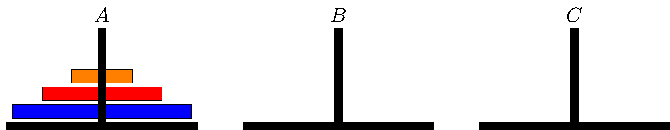
\includegraphics[width=4in]{ch09/images/ht0.pdf}
  \end{figure}
\end{frame}

\begin{frame}
  \begin{figure}[htbp]
    \centering
    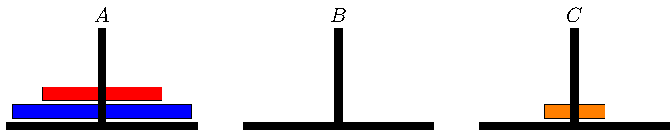
\includegraphics[width=4in]{ch09/images/ht1.pdf}
  \end{figure}
\end{frame}

\begin{frame}
  \begin{figure}[htbp]
    \centering
    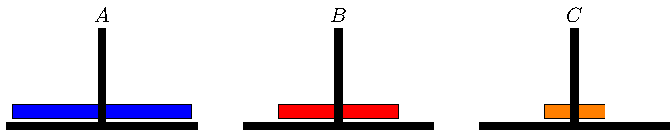
\includegraphics[width=4in]{ch09/images/ht2.pdf}
  \end{figure}
\end{frame}

\begin{frame}
  \begin{figure}[htbp]
    \centering
    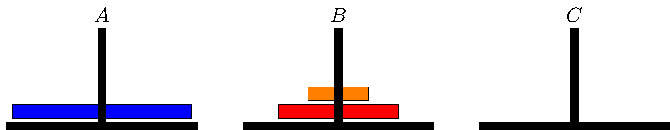
\includegraphics[width=4in]{ch09/images/ht3.pdf}
  \end{figure}
\end{frame}

\begin{frame}
  \begin{figure}[htbp]
    \centering
    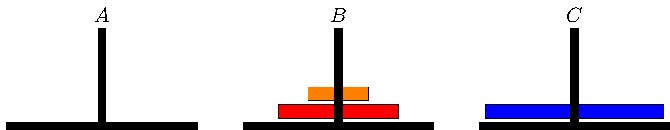
\includegraphics[width=4in]{ch09/images/ht4.pdf}
  \end{figure}
\end{frame}

\begin{frame}
  \begin{figure}[htbp]
    \centering
    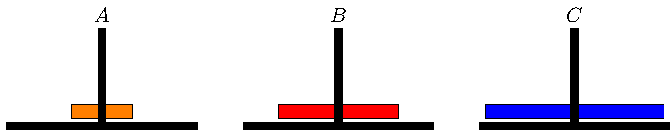
\includegraphics[width=4in]{ch09/images/ht5.pdf}
  \end{figure}
\end{frame}

\begin{frame}
  \begin{figure}[htbp]
    \centering
    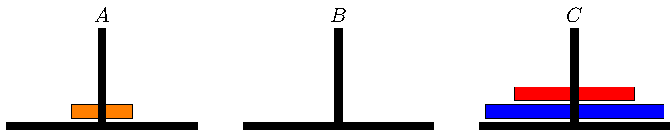
\includegraphics[width=4in]{ch09/images/ht6.pdf}
  \end{figure}
\end{frame}

\begin{frame}
  \begin{figure}[htbp]
    \centering
    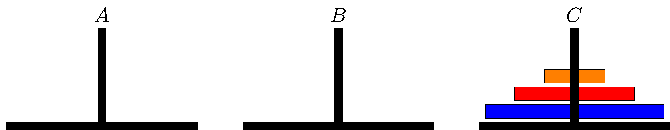
\includegraphics[width=4in]{ch09/images/ht7.pdf}
  \end{figure}
\end{frame}

  }{}
  \ifthenelse{\equal{#1}{o10}}{
    \section{数组与指针}

\begin{frame}[fragile]\ft{\secname}
\begin{biancheng} 
  编写一个函数,对数组按从小到大进行排序。简单排序算法原理:每次从左至右扫描序列,记下最小值的位置。
\end{biancheng}
\end{frame}


\begin{frame}[fragile,allowframebreaks]\ft{\secname}
\lstinputlisting
{ch10/code/ex10_01.c}
\end{frame}


\begin{frame}[fragile]\ft{\secname}
\begin{biancheng} 
编写一个程序,初始化一个\lstinline| double |数组,然后把数组内容复制到另外两个数组。
\begin{itemize}
\item 制作第一份拷贝的函数使用数组符号;
\item 制作第二份拷贝的函数使用指针符号,并使用指针的增量操作。
\item 把目标数组名和要复制的元素个数作为参数传递给函数。
\item 对一个长度为7的数组,请利用以上函数将其第3到第5个元素复制到一个长度为3的数组中。
\end{itemize}
\end{biancheng}
% \begin{lstlisting}
% double source[5] = {1.1, 2.2, 3.3, 4.4, 5.5};
% double target1[5], target2[5];
% copy_arr(source, target1, 5);
% copy_ptr(source, target2, 5);
% \end{lstlisting}
\end{frame}

\begin{frame}[fragile,allowframebreaks]\ft{\secname}
\lstinputlisting
{ch10/code/ex10_02.c}
\end{frame}

 



\begin{frame}[fragile]\ft{\secname}
\begin{biancheng} 
编写一个函数,求一个\lstinline| double |数组的最大值及其下标。
\end{biancheng}
\end{frame}

\begin{frame}[fragile,allowframebreaks]
\lstinputlisting
[language=c,numbers=left,frame=single]
{ch10/code/ex10_03.c}
\end{frame}

 

\begin{frame}[fragile]\ft{\secname}
\begin{biancheng} 
编写一个函数,将两个长度相同的数组相加,结果存储到第三个数组中。
\end{biancheng}
\end{frame}

\begin{frame}[fragile,allowframebreaks]\ft{\secname}
\lstinputlisting
[language=c,numbers=left,frame=single]
{ch10/code/ex10_04.c}
\end{frame}


 


\begin{frame}[fragile]\ft{\secname}
\begin{biancheng} 
编写一个函数,求两个三维向量的内积和外积。
\end{biancheng}
设
$$
\vec u = (a_1,a_2,a_3)^T, ~~~ 
\vec v = (b_1,b_2,b_3)^T
$$
则内积为
$$
\vec u \cdot \vec v = a_1b_1+a_2b_2+a_3b_3
$$
外积为
$$
\vec u \times \vec v = 
\left|
\begin{array}{ccc}
\mathbf i & \mathbf j & \mathbf k \\
a_1 & a_2 & a_3 \\
b_1 & b_2 & b_3
\end{array}
\right| = (a_2b_3-a_3b_2, a_3b_1-a_1b_3, a_1b_2-a_2b_1)^T.
$$
\end{frame}

\begin{frame}[fragile,allowframebreaks]\ft{\secname}
\lstinputlisting
[language=c,numbers=left,frame=single]
{ch10/code/ex10_05.c}
\end{frame}



\begin{frame}[fragile]
\begin{biancheng} 
编写一个函数,提示用户输入三个数集,每个数集包括5个\lstinline| double |值。程序应当实现以下功能:
\begin{enumerate}
\item 把输入信息存储到一个$3\times5$的数组中
\item 计算出每个数集的平均值
\item 计算所有数的平均值
\item 找出这$15$个数中的最大值
\item 打印出结果
\end{enumerate}
\end{biancheng}
\end{frame}

% \begin{frame}[fragile,allowframebreaks]
% \lstinputlisting
% [language=c,numbers=left,frame=single]
% {ch10/code/ex10_12.h}
% \end{frame}

% \begin{frame}[fragile,allowframebreaks]
% \lstinputlisting
% [language=c,numbers=left,frame=single]
% {ch10/code/ex10_12.c}
% \end{frame}

  

\begin{frame}[fragile]
\begin{biancheng} 
用变长数组重写以上程序。
\end{biancheng}
\end{frame}

\begin{frame}[fragile]
\begin{biancheng} 
用一维数组重写以上程序。
\end{biancheng}
\end{frame}

  }{}
  \ifthenelse{\equal{#1}{o11}}{
    \section{字符串与字符串函数}
\begin{frame}[fragile]
\begin{li} 
设计并测试一个函数\lstinline| my_strchr()|,其功能是搜索第一个参数指定的字符串,在其中查找由第二个参数指定的字符首次出现的位置。
\begin{itemize}
\item 若找到,返回指向这个字符的指针;
\item 若没有找到,返回\lstinline| NULL|。
\end{itemize}
\end{li}
\end{frame}


\begin{frame}[fragile,allowframebreaks]
\lstinputlisting
[language=c,numbers=left,frame=single]
{ch11/code/my_strchr.c}
\end{frame}


\begin{frame}[fragile]
\begin{li} 
编写一个函数\lstinline| is_within()|,判断指定字符是否在指定字符串中。
\begin{itemize}
\item 若在其中,则返回\lstinline|true|;
\item 否则返回\lstinline|false|。
\end{itemize}
\end{li}
\end{frame}


\begin{frame}[fragile,allowframebreaks]
\lstinputlisting
[language=c,numbers=left,frame=single]
{ch11/code/is_within.c}
\end{frame}

\begin{frame}[fragile]
\begin{li} 
函数\lstinline|strncpy(s1, s2, n)|从\lstinline| s2 |复制\lstinline| n |个字符给\lstinline| s1 |。
\begin{itemize}
\item 若\lstinline| s2 |的长度大于或等于\lstinline| n |,则目标字符串没有标识结束的空字符。
\item 函数返回{\tf s1}。
\end{itemize}
请自行编写该函数,取名为\lstinline| my_strncpy() |。
\end{li}
\end{frame}


\begin{frame}[fragile,allowframebreaks]
\lstinputlisting
[language=c,numbers=left,frame=single]
{ch11/code/my_strncpy.c}
\end{frame}




\begin{frame}[fragile]
\begin{li} 
编写函数\lstinline| my_strstr() |,它接受两个字符串指针参数。
\begin{itemize}
\item 若第二个字符串被包含在第一个字符串中,则返回被包含的字符串开始的地址。
\item 如,\lstinline| my_strstr("hats","at") |返回\lstinline|"hats"|中\lstinline|'a'|的地址,否则返回\lstinline| NULL |。
\end{itemize}
\end{li}
\end{frame}


\begin{frame}[fragile,allowframebreaks]
\lstinputlisting
[language=c,numbers=left,frame=single]
{ch11/code/my_strstr.c}
\end{frame}


  }{}
  \ifthenelse{\equal{#1}{s1}}{
    %%%%
\begin{frame}[fragile]
\begin{figure}
\centering

\includegraphics[width=3in]{ch01/fig/helloworld}
\end{figure}

\lstinputlisting[]{ch01/code/helloworld.c}

\end{frame}

%%%%
\begin{frame}
\begin{figure}
\centering

\includegraphics[width=2.in]{ch01/fig/cprimerplus}
\end{figure}
\end{frame}
    \section{计算机硬件}


%\begin{frame}\ft{\subsecname}
%\begin{figure}
%\centering
%\animategraphics[height=2.in,autoplay,controls,buttonsize=0em,loop]{12}{ch01/fig/computer_}{0}{3}
%\end{figure}
%\end{frame}

 

\begin{frame}\ft{硬件}
\begin{itemize}
\item 中央处理器(Central Processing Unit, CPU) \\
\item 存储器 \\
\begin{itemize}
	\item 内存(Memory) \\
	\item 外存 
	\begin{AutoMultiColItemize}
		\item 硬盘
		\item 软盘
		\item 光盘
		\item U盘
	\end{AutoMultiColItemize}
\end{itemize}
\item 输入设备 
\begin{AutoMultiColItemize}
	\item 键盘
	\item 鼠标
	\item 摄像头
	\item 扫描仪
\end{AutoMultiColItemize}
\item 输出设备\begin{AutoMultiColItemize}
	\item 显示器
	\item 打印机
	\item 音响
	\item 绘图仪
\end{AutoMultiColItemize}
\end{itemize}
\end{frame}

\begin{frame}[fragile]\ft{主板}
\begin{figure}[h] 
	\centering
	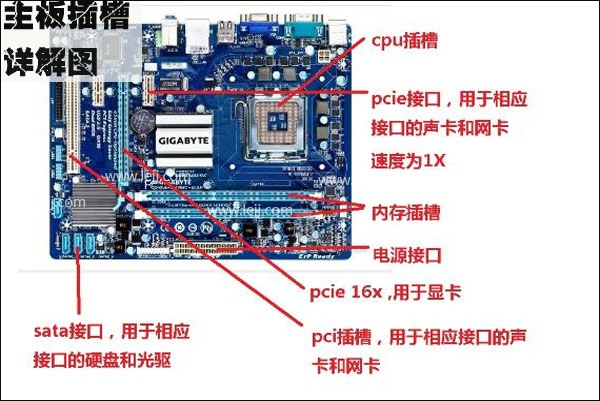
\includegraphics[width=\textwidth]{ch01/fig/mobo}
\end{figure}
\end{frame}


\begin{frame}\ft{主板}
{CPU、内存、硬盘、显卡、声卡等都安装在\red{主板}上。}

\begin{itemize}
\item
将电脑的各个部件连接起来。 \\[0.1in]
\item
提供各种外接设备的接口,如:
\begin{AutoMultiColItemize}
\item USB接口
\item 键盘接口
\item 鼠标接口
\item 网线接口
\end{AutoMultiColItemize}
\end{itemize}
\end{frame}






\begin{frame}[fragile]\ft{CPU}
\begin{figure}[h] 
\begin{minipage}[t]{0.45\linewidth}
\centering

\includegraphics[width=\textwidth]{ch01/fig/cpu1}
\end{minipage}
\hfill
\begin{minipage}[t]{0.45\linewidth}
\centering
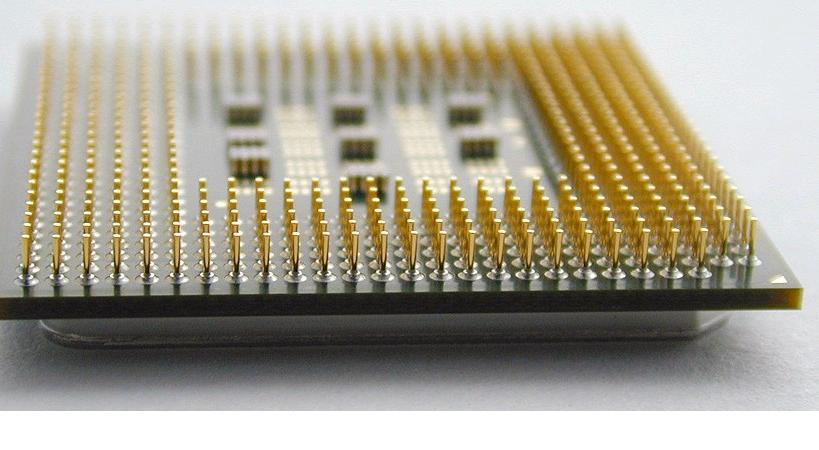
\includegraphics[width=\textwidth]{ch01/fig/cpu2}
\end{minipage}
\end{figure}
\end{frame}

\begin{frame}\ft{CPU}
CPU是计算机的大脑。

\red{计算机处理数据的能力主要取决于CPU。}  \vspace{.1in}

三种基本操作: 

\begin{itemize}
\item \red{读数据}:一般从内存读取数据。 \\[0.1in]
\item \red{处理数据}:通过算术逻辑单元对数据进行处理。 \\[0.1in]
\item \red{写数据}:将数据写入内存。
\end{itemize}

\end{frame}

\begin{frame}\ft{CPU}
 
CPU一般由以下四部分组成:
\begin{itemize}
\item  \red{运算器(算术逻辑单元)} \quad 处理数据 
\begin{itemize}
\item 算术运算:加、减、乘、除 
\item 逻辑运算:与、或、非、异或
\end{itemize} 
\item  \red{控制器}  \quad 对指令译码,并且发出为完成每条指令所要执行的各个操作的控制信号。\\[.1in]
\item  \red{寄存器}  \quad 保存指令执行过程中临时存放的寄存器操作数和中间(或最终)的操作结果。 
\begin{AutoMultiColItemize}
\item 通用寄存器
\item 专用寄存器
\item 控制寄存器
\end{AutoMultiColItemize}

\item \red{高速缓冲存储器} \quad 在CPU芯片内,是一个读写速度比内存更快的存储器。
%当CPU向内存中写入或读出数据时,这个数据也被存储进高速缓冲存储器中。当CPU再次需要这些数据时,CPU就从高速缓冲存储器读取数据,而不是访问较慢的内存,当然,如需要的数据在Cache中没有,CPU会再去读取内存中的数据。
\end{itemize}
\end{frame}
 
\begin{frame}\ft{内存}
\begin{figure}
\centering
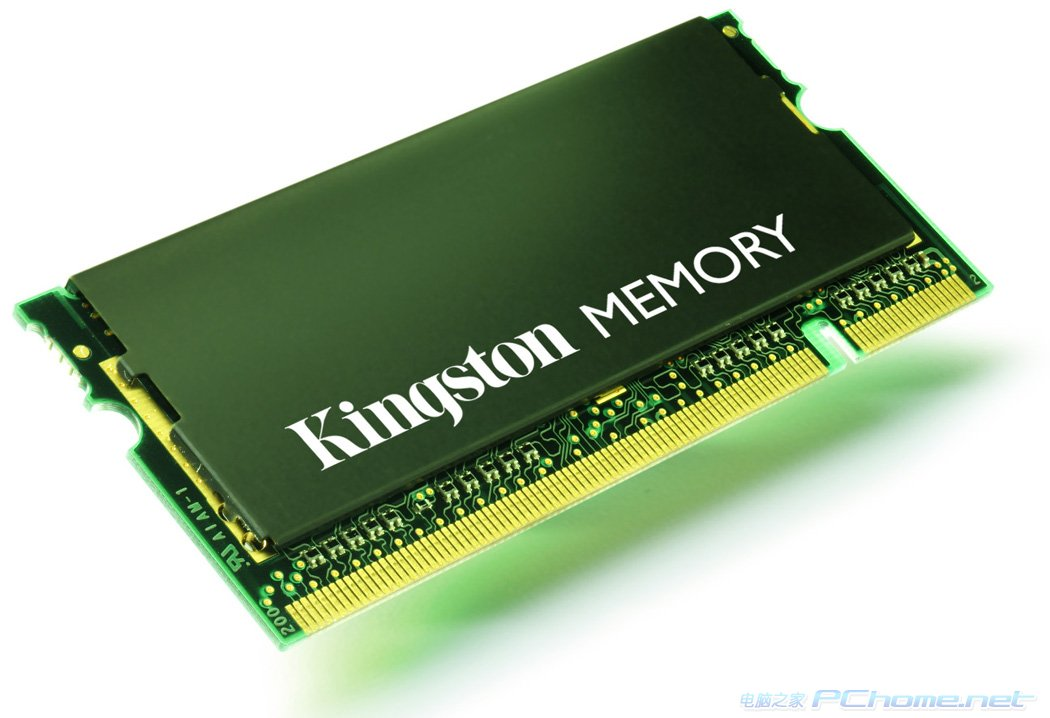
\includegraphics[width=3in]{ch01/fig/memory} 
\end{figure}
\end{frame}
 
\begin{frame}\ft{内存}
\begin{itemize}
\item 内存是CPU能直接寻址的存储空间,所有程序的运行都是在内存中进行的。\\[0.1in]
\item
只要计算机在运行中,CPU就会把需要运算的数据调到内存中进行运算,当运算完成后CPU再将结果传送出来。\\[0.1in]
\item
其作用是用于暂时存放CPU中的运算数据,以及与硬盘等外部存储器交换的数据。\\[0.1in]
\end{itemize}
 \end{frame}
 
 \begin{frame}\ft{内存}
 

\begin{itemize}
\item \red{只读存储器(Read Only Memory, ROM)} 
\item[] 只能读取,不能写入。即使断电,里面的数据也不会丢失,一般用于存放计算机的基本程序和数据。\\[0.1in] 
\item \red{随机存储器(Random Access Memory, RAM)}
\item[] 既可读取,也可写入。断电时,里面的数据就会丢失。{内存条就是将RAM集成块集中在一起的一小块电路板。}\\[0.2in]

\end{itemize}
 \end{frame}
 
\begin{frame}[fragile]\ft{各类存储器的逻辑连接}
\begin{figure}[h] 
\centering
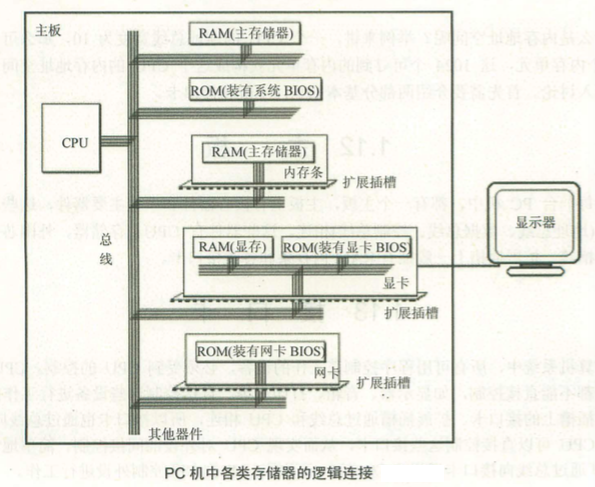
\includegraphics[width=3.7in]{ch01/fig/PCLink}
\end{figure}
\end{frame}

    \section{计算机基本软件}

\begin{frame}\ft{\secname}
软件是组成计算机系统的重要部分。

\begin{itemize}
\item 
\red{系统软件}\quad 计算机生产厂商提供的基本软件,如
\begin{AutoMultiColItemize}
\item 操作系统
\item 文字处理程序
\item 计算机语言处理程序
\item 数据库管理程序 
\end{AutoMultiColItemize} 
\item \red{应用软件}\quad 
为满足用户不同领域、不同问题的应用需求而提供的那部分软件,如
\begin{AutoMultiColItemize}
	\item 多媒体软件
	\item 社交软件
	\item 办公软件
	\item 商务软件 
\end{AutoMultiColItemize} 
\end{itemize}
\red{系统软件依赖于机器,而应用软件则更接近用户业务。}
\end{frame}

\begin{frame}\ft{操作系统(OS)}
\begin{itemize}
\item 最基本也是最重要的系统软件。\\[0.1in]
\item \red{功能}\\[0.1in]
\begin{itemize}
	\item 管理计算机系统的各种硬件资源;\\[0.1in]
	\item 解释用户对机器的管理命令,使它转换为机器实际的操作。\\[0.1in]
\end{itemize} 
\item \red{常见的操作系统}\\[0.1in]
\begin{itemize}
	\item DOS \\
	\item WINDOWS \\
	\item UNIX(LINUX) \\
	\item OS X \\
\end{itemize}
\end{itemize}
\end{frame}

\begin{frame}\ft{计算机语言}
计算机语言分为:

\begin{itemize}
\item \red{机器语言}\quad 机器能直接识别的语言,是由“1”和“0”组成的一组代码指令。\\[0.1in]
\item \red{汇编语言}\quad 与机器语言指令一一对应的符号指令和简单语法。\\[0.1in]
\item \red{高级语言}\quad 比较接近日常用语,对机器依赖性低,即适用于各种机器的计算机语言,如
\begin{AutoMultiColItemize}
\item Visual Basic
\item Fortran
\item C/C++
\item Java
\item Python
\item matlab
\end{AutoMultiColItemize}
\end{itemize}
\end{frame}

\begin{frame}\ft{计算机语言}

将高级语言翻译为机器语言,有两种方式: \vspace{0.05in}

\begin{itemize}
\item\red{编译} \\[0.1in]
\begin{itemize}
	\item \red{工作原理}\quad 把高级语言程序作为一个整体进行处理,编译后与子程序库连接,形成一个完整的可执行程序 \\[0.1in]
	\item \red{缺点}\quad 编译、链接比较费时\\[0.1in]
	\item \red{优点}\quad 可执行程序运行速度很快 \\[0.1in]
	\item \red{适用语言}\quad Fortran、C/C++ \\[0.1in]
\end{itemize}

\item\red{解释} \\[0.1in]
\begin{itemize}
	\item \red{工作原理}\quad 对高级语言程序逐句解释执行\\[0.1in]
	\item \red{缺点}\quad 运行效率较低\\[0.1in]
	\item \red{优点}\quad 程序设计的灵活性大\\[0.1in]
	\item \red{适用语言}\quad Basic、Python、Matlab
\end{itemize}
\end{itemize}
\end{frame}
    \section{数制}

\begin{frame}\ft{\secname}
\begin{dingyi}[数制]
用一组固定的符号和统一的规则来表示数值的方法。
\end{dingyi}
\vspace{0.2in}

\red{常用的数制:}
\begin{AutoMultiColItemize}
\item 十进制
\item 二进制
\item 八进制
\item 十六进制
\end{AutoMultiColItemize}


在一种数制中,只能使用一组\red{固定的数字符号}来表示数目的大小。

\red{具体使用多少个数字符号来表示数目的大小,就称为该数制的基数。}
\end{frame}

\begin{frame}\ft{\secname}

\begin{table}
\begin{tabular}{ccccc}\hline
&基数&数字符号&最小数码&最大数码\\\hline
二进制(Binary)&2&0,1&0&1\\[.1in]
八进制(Octal)&8&0-7&0&7\\[.1in]
十进制(Decimal)&10&0-9&0&9\\[.1in]
十六进制(Hexadecimal)&16&0-9,A-F&0&F\\\hline
\end{tabular}
\end{table}

\end{frame}



\begin{frame}\ft{\secname}
{既然有不同的进制,那么在给出一个数时,需指明是什么数制里的数。}
\vspace{0.1in}

如:$(1010)_2,~(1010)_8,~(1010)_{10},~(1010)_{16}$所代表的数值就不同。\vspace{0.15in}

{除了用下标表示外,还可用后缀字母来表示数制。}
\vspace{0.1in}

如:1A4EH,~FEEDH,~BADH与$\mbox{(1A4E)}_{16},~\mbox{(FEED)}_{16},~\mbox{(BAD)}_{16}$的意义相同。
\end{frame}

\begin{frame}\ft{\secname}
\begin{figure}[h]
\centering
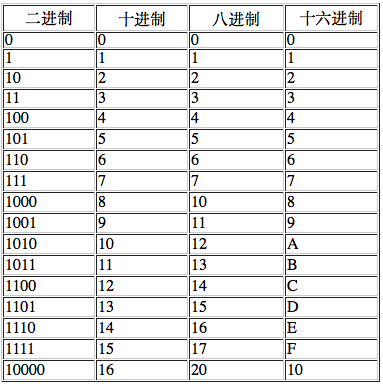
\includegraphics[width=3.in]{ch01/fig/shuzhi}
\end{figure}
\end{frame}

\begin{frame}\ft{进制}
{在数制中,N进制必须是逢N进一。}

\begin{itemize}
\item 十进制数:\red{逢十进一}。
\[
(1010)_{10}=1\times10^3+0\times10^2+1\times10^1+0\times10^0
\]
\item 二进制数:\red{逢二进一}。
\[
(1010)_{2}=1\times2^3+0\times2^2+1\times2^1+0\times2^0=(10)_{10}
\]
\item 八进制数:\red{逢八进一}。
\[
(1010)_{8}=1\times8^3+0\times8^2+1\times8^1+0\times8^0=(520)_{10}
\]
\item 十六进制数:\red{逢十六进一}。
\[
\mbox{(BAD)}_{16}=11\times16^2+10\times16^1+13\times16^0=(2989)_{10}
\]
\end{itemize}
\end{frame}

\begin{frame}\ft{二进制数的加法法则}

\[
\boxed{
\begin{array}{l}
0+0=0\\
0+1=1\\
1+0=1\\
1+1=10\\
1+1+1=10+1=11
\end{array}
}
\]

\begin{table}
\centering
\begin{tabular}{cD{.}{.}{3}}
&1011\\
+&1010\\
\hline
=&10101
\end{tabular}
\end{table}
\end{frame}

\begin{frame}\ft{二进制数的减法法则}

\[
\boxed{
\begin{array}{rl}
0-0=0&\\
1-0=1&\\
1-1=0&\\
0-1=1&\mbox{有借位,借1当$(10)_2$}\\
0-1-1=0&\mbox{有借位}\\
1-1-1=1&\mbox{有借位}\\
\end{array}
}
\]

\begin{table}
\centering
\begin{tabular}{cD{.}{.}{3}}
%&111110\\
&1~1~0~0~0~0\\
-&1~0~1~1~1\\
\hline
=&1~1~0~0~1
\end{tabular}
\end{table}
\end{frame}

\begin{frame}\ft{二进制的乘法法则}

\[\boxed{
\begin{array}{rr}
0\times0=0, & 
0\times1=0\\
1\times0=0, & 
1\times1=1\\
\end{array}
}
\]

\begin{table}
\centering
\begin{tabular}{cD{.}{.}{3}}
%&111110\\
&1~1~1~0\\
$\times$&0~1~1~0\\
\hline
&0~0~0~0\\
&1~1~1~0~~~\\
&1~1~1~0~~~~~\\
+&0~0~0~0~~~~~~~~\\
\hline
&1~0~1~0~1~0~0
\end{tabular}
\end{table}

\end{frame}
%
\begin{frame}\ft{二进制的除法法则}

\begin{figure}
\centering
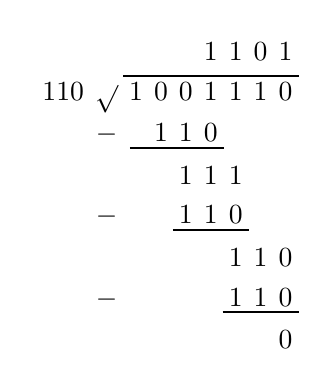
\begin{tikzpicture}
\matrix[ampersand replacement=\&,matrix of math nodes,nodes={inner sep=0.2em}]{
    \& \& \& \&  \& 1 \& 1 \& 0 \& 1\\[4pt]
110 \& \sqrt{} \& |(a)|1\& 0 \& 0\& 1 \& 1 \& 1 \& |(b)| 0 \\
    \& - \&  |(c)| \&  1 \& 1\& |(d)|0  \&  \&  \&   \\[4pt]
    \&   \&   \&   \& 1\& 1  \& 1\&  \&   \\[4pt]
    \& - \&   \&   \& |(e)|1\& 1  \& |(f)|0\&  \&   \\[4pt]
    \&   \&   \&   \&  \&    \& 1\& 1\& 0  \\[4pt]
    \& - \&   \&   \&  \&    \& |(g)|1\& 1\& |(h)|0  \\[4pt]
    \&   \&   \&   \&  \&    \&  \&  \& 0  \\[4pt]
};
\draw[thick] (a.north west) -- (b.north east)
      (c.south west) -- (d.south east)
      (e.south west) -- (f.south east)
      (g.south west) -- (h.south east);

\end{tikzpicture}
\end{figure}
\end{frame}

\begin{frame}\ft{十进制数到二进制数的转换}

{(1)整数部分} 除2取余,直至商为0,最后将所得余数按逆序排列。 \vspace{0.1in}

\begin{figure}
\centering
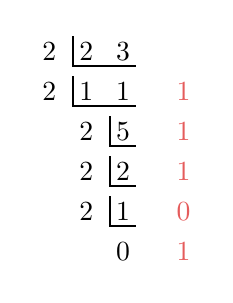
\begin{tikzpicture}
\matrix[ampersand replacement=\&,matrix of math nodes,column sep=1ex,nodes={inner sep=0.2em}]{
    2  \& |(a)|  2 \& |(b)|3 \& \& \& \\[4pt]
    2  \& |(c)|  1 \& |(d)|1 \& \& \& \red{1}\\[4pt]
       \&        2 \& |(e)|5 \& \& \& \red{1}\\[4pt]
       \&        2 \& |(f)|2 \& \& \& \red{1}\\[4pt]
       \&        2 \& |(g)|1 \& \& \& \red{0}\\[4pt]
       \&          \&      0 \& \& \& \red{1}\\[4pt]
};
\draw[thick] (a.north west)--(a.south west)--(b.south east)
(c.north west)--(c.south west)--(d.south east)
(e.north west)--(e.south west)--(e.south east)
(f.north west)--(f.south west)--(f.south east)
(g.north west)--(g.south west)--(g.south east);

\end{tikzpicture}
\end{figure}
结果为
$
(23)_{10}=(10111)_2.
$
\end{frame}
%
\begin{frame}\ft{十进制数到二进制数的转换}

{(2)小数部分} 乘2取整数,若小数部分是5的倍数,则以最后小数部分为0为止,否则以约定的精确度为准,最后将所取整数按顺序排列。 \vspace{0.1in}

\begin{figure}
\centering
\begin{tikzpicture}
\matrix[ampersand replacement=\&,matrix of math nodes,column sep=1ex,nodes={inner sep=0.2em}]{
            \& 0 \& .\& 2\& 5      \& \&  \\[4pt]
|(a)|\times \&   \&  \&  \& |(b)|2 \& \&   \\[4pt]
            \& 0 \& .\& 5\& 0      \& \& \mbox{取整数位}0 \\[4pt]
|(c)|\times \&   \&  \&  \& |(d)|2 \& \&   \\[4pt]
            \& 1 \& .\& 0\& 0      \& \& \mbox{取整数位}1  \\[4pt]        
};
\draw[thick] (a.south west)--(b.south east)
(c.south west)--(d.south east);
\end{tikzpicture}
\end{figure}

结果为
$
(0.25)_{10}=(0.01)_2.
$

\end{frame}
%
\begin{frame}\ft{十进制数到二进制数的转换}
\begin{li}
将十进制数$125.24$转换为二进制数(取四位小数)。
\end{li}
\pause 

\begin{figure}
\begin{minipage}[t]{0.45\linewidth}
\centering
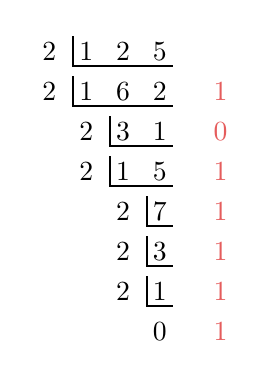
\begin{tikzpicture}[scale=0.8]
\matrix[ampersand replacement=\&,matrix of math nodes,column sep=1ex,nodes={inner sep=0.2em}]{
    2  \& |(a)|  1 \&       2 \& |(b)|5 \& \& \& \\[4pt]
    2  \& |(c)|  1 \&       6 \& |(d)|2 \& \& \& \red{1}\\[4pt]
       \&        2 \& |(e1)|3 \& |(e)|1 \& \& \& \red{0}\\[4pt]
       \&        2 \& |(f1)|1 \& |(f)|5 \& \& \& \red{1}\\[4pt]
       \&          \&       2 \& |(g)|7 \& \& \& \red{1}\\[4pt]
       \&          \&       2 \& |(h)|3 \& \& \& \red{1}\\[4pt]
       \&          \&       2 \& |(i)|1 \& \& \& \red{1}\\[4pt]       
       \&          \&         \&      0 \& \& \& \red{1}\\[4pt]
};
\draw[thick] (a.north west)--(a.south west)--(b.south east)
(c.north west)--(c.south west)--(d.south east)
(e1.north west)--(e1.south west)--(e.south east)
(f1.north west)--(f1.south west)--(f.south east)
(g.north west)--(g.south west)--(g.south east)
(h.north west)--(h.south west)--(h.south east)
(i.north west)--(i.south west)--(i.south east);

\end{tikzpicture}
\end{minipage}
\hfill
\begin{minipage}[t]{0.45\linewidth}
\centering
\begin{tikzpicture}[scale=0.8]
\matrix[ampersand replacement=\&,matrix of math nodes,column sep=1ex,nodes={inner sep=0.1em}]
{
            \& 0 \& .\& 2\& 4      \& \&  \\[4pt]
|(a)|\times \&   \&  \&  \& |(b)|2 \& \&   \\[4pt]
            \& 0 \& .\& 4\& 8      \& \& \mbox{取整数位}0 \\[4pt]
|(c)|\times \&   \&  \&  \& |(d)|2 \& \&   \\[4pt]
            \& 0 \& .\& 9\& 6      \& \& \mbox{取整数位}0  \\[4pt]
|(e)|\times \&   \&  \&  \& |(f)|2 \& \&   \\[4pt]
            \& 1 \& .\& 9\& 2      \& \& \mbox{取整数位}1  \\[4pt]                    
|(g)|\times \&   \&  \&  \& |(h)|2 \& \&   \\[4pt]
            \& 1 \& .\& 8\& 4      \& \& \mbox{取整数位}1  \\[4pt]            
};
\draw[thick] (a.south west)--(b.south east)
(c.south west)--(d.south east)
(e.south west)--(f.south east)
(g.south west)--(h.south east);
\end{tikzpicture}
\end{minipage}
\end{figure}
\pause 
结果为
$$
(125.24)_{10}=(1111101.0011)_2.
$$
\end{frame}
%
\begin{frame}\ft{二进制数到十进制数的转换}

{基本原理:} 
\begin{itemize}
\item 将二进制数从小数点开始,往左从$0$开始对各位进行正序编号,往右序号则分别为$-1,-2,-3,\cd$,直到最末位。\\[0.1in]
\item 然后分别将各位上的数乘以$2$的$k$次幂所得的值进行求和,其中$k$的值为各个位所对应的上述编号。
\end{itemize}
\end{frame}

\begin{frame}\ft{二进制数到十进制数的转换}
\begin{li}
将二进制数$1101.101$转换为十进制数(取四位小数)。
\end{li}
\pause 
$$
\begin{array}{rl}
& (1101.101)_2 \\[0.1in]
= & 1\times2^3+1\times2^2+0\times2^1+1\times2^0
+1\times2^{-1}+0\times2^{-2}+1\times2^{-3}\\[0.1in]
= & 8+4+1+0.5+0.125\\[0.1in]
= & 13.625
\end{array}
$$
\end{frame}
%
\begin{frame}\ft{二进制数到十六进制数的转换}

{基本原理:} 由于十六进制数基数是2的四次幂,所以一个二进制转换为十六进制,
\begin{itemize}
\item
如果是整数,只要从它的低位到高位每$4$位组成一组,然后将每组二进制数所对应的数用十六进制表示出来。\\[0.1in]
\item
如果有小数部分,则从小数点开始,分别向左右两边按照上述方法进行分组计算。
\end{itemize}
\end{frame}
%
\begin{frame}\ft{二进制数到十六进制数的转换}
\begin{li}
将二进制数$11~1010~1111~0001~0111$转换为十六进制数。
\end{li}
\pause 
\begin{table}
\centering
\begin{tabular}{cccccc}\hline
二进制数&$11$&$1010$&$1111$&$0001$&$0111$\\[0.1in]
十六进制数&$3$&$A$&$F$&$1$&$7$\\ \hline
\end{tabular}
\end{table}
结果为
$$
(11~1010~1111~0001~0111)_2=(3AF17)_{16}
$$
\end{frame}
%
%

    \section{汇编语言简介}

\begin{frame}\ft{机器语言}
机器语言是机器指令的集合。机器指令是计算机可以正确执行的命令,它是一组二进制数字。计算机将其转变为一组高低电平,以使电子器件收到驱动,进行运算。
\end{frame}

\begin{frame}[fragile]\ft{机器语言}
8086CPU完成运算 \lstinline| s=768+12288-1280 |的机器码如下:
\begin{lstlisting}[frame=no]
1011 0000 0000 0000 0000 0011 
0000 0101 0000 0000 0011 0000 
0010 1101 0000 0000 0000 0101
\end{lstlisting}

\pause
若将程序错写成以下形式,请指出错误:
\begin{lstlisting}[frame=no]
1011 0000 0000 0000 0000 0011 
0000 0101 0000 0000 0011 0000 
0001 0110 1000 0000 0000 0101
\end{lstlisting}

\end{frame}

\begin{frame}\ft{机器语言}
书写和阅读机器码程序不是一件简单的工作,需要记住抽象的二进制码。上面只是一个非常简单的小程序,就暴露了机器码的晦涩难懂和不易查找。\vspace{0.1in}

早期程序员很快发现了使用机器语言带来的麻烦,于是汇编语言产生了。

\end{frame}

\begin{frame}\ft{\secname}
汇编语言的主体是汇编指令。汇编指令和机器指令的差别在于指令的表示方法上。{汇编指令是机器指令便于记忆的书写形式。} \pause \vspace{0.1in}

\begin{itemize}
\item[]
操作:寄存器 \lstinline|BX| 的内容送到 \lstinline|AX| 中\\
\item[]
机器指令:\lstinline| 1000 1001 1101 1000|\\
\item[]
汇编指令:\lstinline| mov ax, bx |
\end{itemize}
\end{frame}

\begin{frame}\ft{\secname}
\begin{wenti}
计算机只能读懂机器指令,那么如何让计算机执行汇编指令编写的程序呢?
\end{wenti}
\pause 

\begin{itemize}
\item[]
需要用到一个能将汇编指令转换为机器指令的翻译程序,即\red{编译器}。\\[0.1in]
\item[]
程序员用汇编语言写出源程序,再用汇编编译器将其编译为机器码,由计算机最终执行。
\end{itemize}

\begin{figure}
\centering
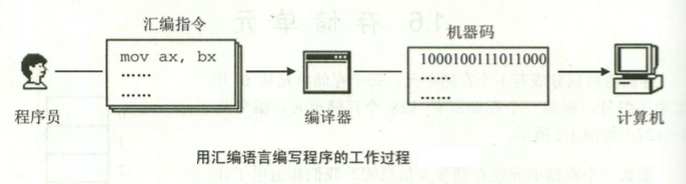
\includegraphics[width=4in]{ch01/fig/asm_process}
\end{figure}
\end{frame}
%
\begin{frame}\ft{存储单元}
存储器被划分为若干个存储单元,每个存储单元从$0$开始顺序编号。例如,假设一个存储器,编号从$0\sim 127$,如下图:
\begin{figure}
\centering
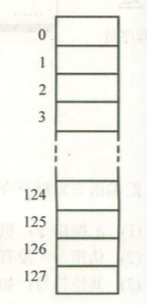
\includegraphics[width=1in]{ch01/fig/cunchudanyuan}
\end{figure}
\end{frame}
%
\begin{frame}\ft{存储单元}

几个概念:

\begin{itemize}
	\item \red{比特(Bit)} \quad 计算机的最小信息单位 \\[.1in]
	\item \red{字节(Byte)} \\[.1in]
	\begin{itemize}
		\item   8个Bit组成1个Byte \\[.1in]
		\item   一个存储单元可存储一个字节,存储器的容量以\red{字节}为最小单位来计算 \\[.1in]
		\item   对于拥有128个存储单元的存储器,其容量为128个字节
	\end{itemize}
	
\end{itemize}
 
对于大容量的存储器,还用以下单位来计算容量(以下用B来代表Byte):
\begin{AutoMultiColItemize}
\item \lstinline|1 KB = 1024 B|   (千)
\item \lstinline|1 MB = 1024 KB|  (兆)
\item \lstinline|1 GB = 1024 KB|  (吉)
\item \lstinline|1 TB = 1024 GB|  (太)
\end{AutoMultiColItemize}
\end{frame}
%
\begin{frame}\ft{CPU对存储器的读写}
\begin{itemize}
\item 首先要指定单元地址。\\[0.1in]
\item 还需要指明\\[0.1in]
\begin{itemize}
	\item 对哪一个存储器进行操作\\[0.1in]
	\item 进行哪种操作\\[0.1in]
	\item 是从中读取数据,还是向里面写入数据
\end{itemize}

\end{itemize}
\end{frame}
%
\begin{frame}\ft{CPU对存储器的读写}
CPU要想进行数据的读写,必须与存储器进行以下3类信息的交互: 

\begin{itemize}
\item \red{地址信息} \quad 存储单元的地址\\[0.1in]
\item \red{控制信息} \quad 器件的选择,以及读或写的命令\\[0.1in]
\item \red{数据信息} \quad 读或写的数据 

\end{itemize}
\end{frame}
%
\begin{frame}\ft{CPU对存储器的读写}
\begin{wenti}
CPU通过什么将地址、数据和控制信息传给存储器芯片呢?
\end{wenti} \pause 
 
计算机传输的信息都是电信号,电信号当然要用导线传送。在计算机中专门有连接CPU和其它芯片的导线,通常称为总线。根据传送信息的不同,总线从逻辑上分为三类: 

\begin{itemize}
\item \red{地址总线} 
\item \red{控制总线}
\item \red{数据总线}
\end{itemize}
\end{frame}
%
\begin{frame}\ft{CPU从内存中读取数据}
\begin{figure}
\centering
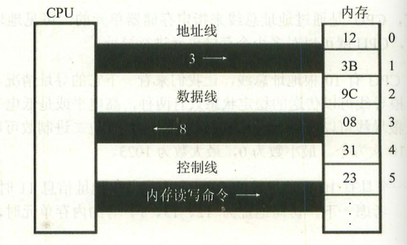
\includegraphics[width=2.5in]{ch01/fig/cpu_read}
\end{figure}
\begin{enumerate}
\item CPU通过\purple{地址总线}将\purple{地址信息$3$}发出;
\item CPU通过\purple{控制总线}发出内存\purple{读命令},选中存储器芯片,并通知它,将要从中读取数据;
\item 存储器将$3$号单元的数据$8$通过\purple{数据总线}送入CPU。
\end{enumerate}
\end{frame}
%
\begin{frame}\ft{CPU对存储器的读写}
写操作与读操作的步骤类似。如向$3$号单元写入数据26。\vspace{0.1in}

\begin{enumerate}
\item CPU通过\purple{地址总线}将\purple{地址信息$3$}发出;
\item CPU通过\purple{控制总线}发出内存\purple{写命令},选中存储器芯片,并通知它,将要从中写入数据;
\item CPU通过\purple{数据总线}将数据$26$送入内存的$3$号单元中。
\end{enumerate}
\end{frame}
%
\begin{frame}\ft{CPU对存储器的读写}
\begin{wenti}
我们知道了CPU如何进行数据的读写。那么,我们又如何命令计算机进行数据的读写呢?
\end{wenti}\pause \vspace{0.1in}

要让计算机工作,应向它输入能驱动其进行工作的电平信息,即机器码。\vspace{0.1in}

\begin{enumerate}
\item[] 机器指令:1010 0001 0000 0011 0000 0000
\item[] 汇编指令:mov ax, [3]
\item[] 含义:传送3号单元的内容入ax。
\end{enumerate}
\end{frame}

\begin{frame}\ft{地址总线}
\begin{itemize}
\item 
CPU通过地址总线指定存储器单元。由此可见,地址总线能传送多少个不同的信息,CPU就可以对多少个存储单元进行寻址。\pause \\[0.1in]
\item 
现假设一个CPU有10根地址总线,可以传送10位二进制数据,共$2^{10}$个不同数据,最小为$0$,最大为$1023$。\pause \\[0.1in]
\item 
一个CPU有$N$根地址线,则称CPU的地址总线的宽度为$N$,最多可以寻找$2^N$个内存单元。
\end{itemize}
\end{frame}
%
\begin{frame}\ft{地址总线}

\begin{figure}
\centering
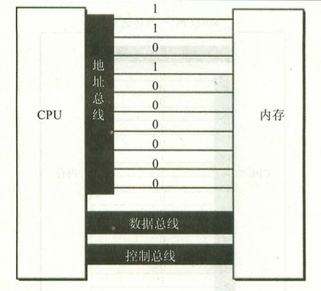
\includegraphics[width=2.5in]{ch01/fig/dizhizongxian}
\caption{地址总线发送的地址信息}
\end{figure}

\end{frame}
%
\begin{frame}\ft{数据总线}
 
CPU与内存和其它器件之间的数据传输通过数据总线来进行。数据总线的宽度决定了CPU与外界的数据传输速度。 
\end{frame}

\begin{frame}\ft{数据总线}

\begin{figure}
\centering
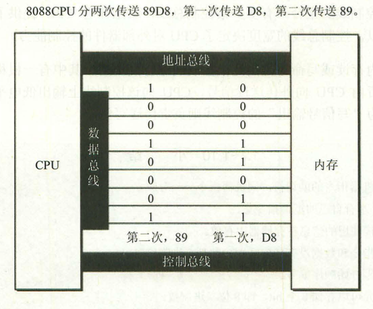
\includegraphics[width=2.5in]{ch01/fig/shujuzongxian1}
\caption{8根数据总线一次可传输一个字节}
\end{figure}

\end{frame}
%
\begin{frame}\ft{数据总线}

\begin{figure}
\centering
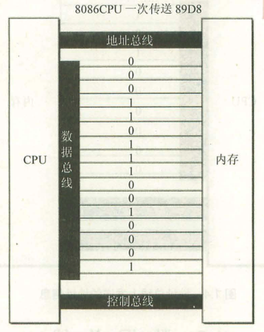
\includegraphics[width=2.in]{ch01/fig/shujuzongxian2}
\caption{16根数据总线一次可传输两个字节}
\end{figure}

\end{frame}

\begin{frame}\ft{控制总线}
 
CPU对外部器件的控制通过控制总线来进行。有多少根控制总线,就意味着CPU提供了对外部器件的多少种控制。因此,控制总线的宽度决定了CPU对外部器件的控制能力。 

\end{frame}

\begin{frame}\ft{寄存器}
一个典型的CPU由运算器、控制器、寄存器等器件构成,这些器件通过内部总线相连。 内部总线实现CPU内部各个器件之间的联系,而外部总线实现CPU与主板上其它器件的联系。 

在CPU中:
\begin{itemize}
\item 运算器进行信息处理;
\item 寄存器进行信息存储;
\item 控制器控制各种器件进行工作;
\item 内部总线连接各种器件,在它们之间进行数据的传送。
\end{itemize}
\end{frame}
%
\begin{frame}\ft{寄存器}
寄存器是CPU中程序员可以用指令读写的部件,程序员通过改变各种寄存器中的内容来实现对CPU的控制。\vspace{0.1in}

不同的CPU,寄存器的个数、结构不尽相同。8086CPU有14个寄存器,每个寄存器都有一个名称,分别是
$$
\mbox{AX、BX、CX、DX、SI、DI、SP、BP、IP、CS、SS、DS、ES、PSW。}
$$
\end{frame}

\begin{frame}\ft{通用寄存器}
8086CPU的所有寄存器都是16位的,可以存放两个字节。\vspace{0.1in}

AX、BX、CX、DX这四个寄存器通常用来存放一般性的数据,被称为通用寄存器。

\begin{figure}
\centering
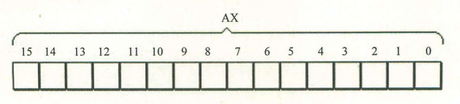
\includegraphics[width=3.5in]{ch01/fig/tongyongjicunqi1}
\caption{16位寄存器的逻辑结构}
\end{figure}


\end{frame}

\begin{frame}\ft{通用寄存器}
\begin{figure}
\centering
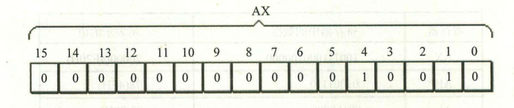
\includegraphics[width=3.5in]{ch01/fig/tongyongjicunqi2}
\caption{$(10010)_2$在寄存器AX中的存储}
\end{figure}
 
\begin{figure}
\centering
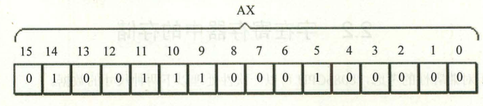
\includegraphics[width=3.5in]{ch01/fig/tongyongjicunqi3}
\caption{$(100111000100000)_2$在寄存器AX中的存储}
\end{figure}
\end{frame}
%
%
%
\begin{frame}\ft{通用寄存器}
\begin{figure}
\centering
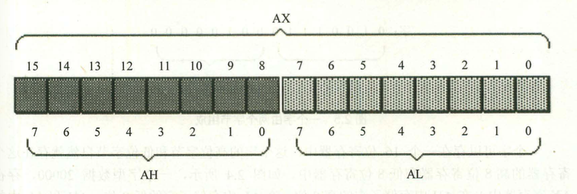
\includegraphics[width=3.5in]{ch01/fig/tongyongjicunqi4}
\caption{16位寄存器可分为两个8位寄存器}
\end{figure}
\end{frame}

\begin{frame}\ft{几条汇编指令}
\begin{figure}
\centering
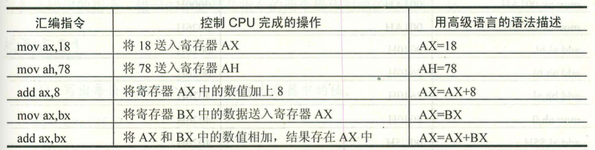
\includegraphics[width=4.5in]{ch01/fig/huibianzhiling1}
\caption{汇编指令举例}
\end{figure}
\end{frame}

\begin{frame}\ft{物理地址}
CPU访问内存单元时,要给出内存单元的地址。所有的内存单元构成的存储空间是一个一维的线性空间,每一个内存单元在这个空间中都有唯一的地址,称为物理地址。\vspace{0.1in}

CPU通过地址总线送入存储器的,必须是一个内存单元的物理地址。在CPU向地址总线上发出物理地址之前,必须要在内部先形成这个物理地址。不同的CPU可以有不同的形成物理地址的方式。
\end{frame}

%\begin{frame}\ft{16位结构的CPU}
%16位结构描述了一个CPU具有以下几个方面的结构特性。\vspace{0.1in}
%
%\begin{itemize}
%\item 运算器一次最多可以处理16位的数据;\\[0.1in]
%\item 寄存器的最大宽度为16位;\\[0.1in]
%\item 寄存器与运算器之间的通路是16位。
%\end{itemize}
%\end{frame}
%
%\begin{frame}\ft{8086CPU给出物理地址的方法}
%8086CPU有20位地址总线,可以传送20位地址,达到1MB寻址能力。\vspace{0.1in}
%
%同时8086CPU是16位结构,在内部一次处理、传输、暂存的地址是16位。
%\vspace{0.1in}
%
%从8086CPU的内部结构来看,若将地址从内部简单出发,只能送出16位的地址,表现出的寻址能力只有64KB。\pause 
%\vspace{0.1in}
%
%\red{8086CPU采用一种在内部用两个16位地址合成的方法来形成一个20位的物理地址。}
%\end{frame}
%
%\begin{frame}\ft{8086CPU给出物理地址的方法}
%\begin{figure}
%\centering
%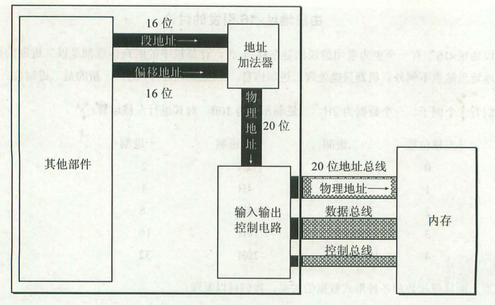
\includegraphics[width=4in]{ch01/fig/xunzhi}
%\caption{8086CPU相关部件的逻辑结构}
%\end{figure}
%\end{frame}
%
%\begin{frame}\ft{8086CPU给出物理地址的方法}
%\begin{figure}
%\centering
%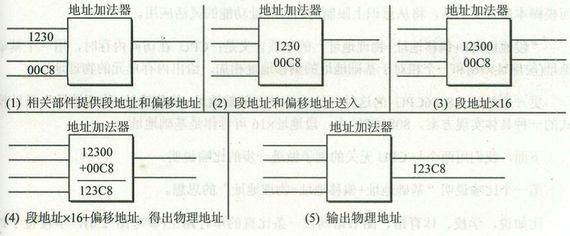
\includegraphics[width=4in]{ch01/fig/xunzhi1}
%\caption{地址加法器的工作过程(物理地址=段地址$\times$16+偏移地址)}
%\end{figure}
%
%\end{frame}
%%
%\begin{frame}\ft{段的概念}
%\begin{figure}
%\centering
%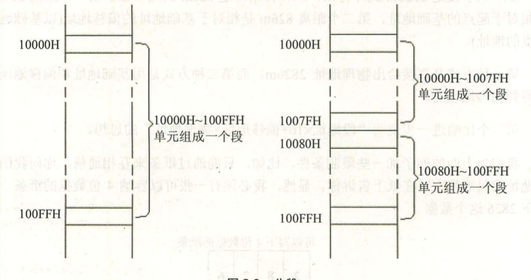
\includegraphics[width=4in]{ch01/fig/duan}
%\caption{内存并没有分段,段的划分来自于CPU,由于8086CPU用“基础地址(段地址$\times$16)+偏移地址”的方式给出内存单元的物理地址,使得我们可以用分段的方式来管理内存。}
%\end{figure}
%\end{frame}
%
%\begin{frame}\ft{段寄存器}
%8086CPU在访问内存时由相关部件提供内存单元的段地址和偏移地址,送入地址加法器合成物理地址。\vspace{0.1in}
%
%段地址在8086CPU的段寄存器中存放。8086CPU有4个段寄存器:CS、DS、SS、ES。\vspace{0.1in}
%
%8086CPU访问内存时由这四个段寄存器提供内存单元的段地址。
%\end{frame}
%
%\begin{frame}\ft{CS和IP}
%CS和IP是8086CPU中两个最关键的寄存器,指示CPU当前要读取指令的地址。
%\vspace{0.1in}
%
%CS为代码段寄存器,IP为指令指针寄存器。
%\vspace{0.1in}
%
%设CS的内容为$M$,IP的内容为$N$,则8086CPU将从内存$M\times16+N$单元开始,读取一条指令并执行。\pause \vspace{0.2in}
%
%\red{以下展示8086CPU读取、执行命令的工作原理:}
%\end{frame}
%
%\begin{frame}\ft{CS和IP}
%
%\begin{figure}
%\centering
%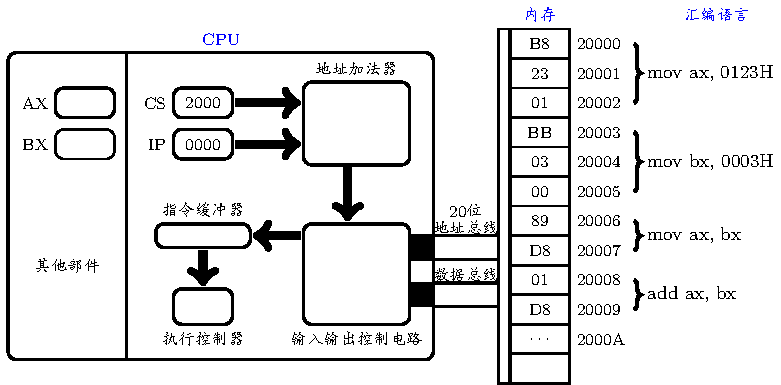
\includegraphics[width=4.5in]{Tikz/csip1}
%\caption{初始状态:CPU将从内存2000:0000处读取指令}
%\end{figure}
%
%\end{frame}
%
%\begin{frame}\ft{CS和IP}
%\begin{figure}
%\centering
%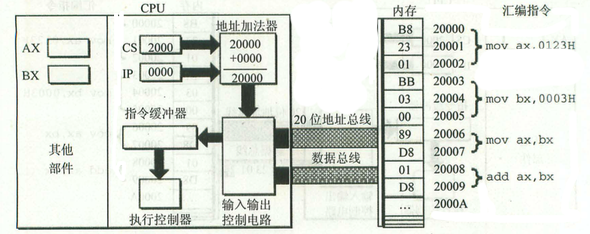
\includegraphics[width=4.5in]{Tikz/csip2}
%\caption{CS、IP中的内容送入地址加法器,形成物理地址}
%\end{figure}
%
%\end{frame}
%
%
%\begin{frame}\ft{CS和IP}
%\begin{figure}
%\centering
%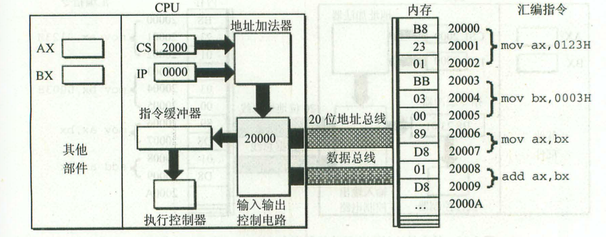
\includegraphics[width=4.5in]{Tikz/csip3}
%\caption{地址加法器将物理地址送至输入输出控制电路}
%\end{figure}
%
%\end{frame}
%
%\begin{frame}\ft{CS和IP}
%\begin{figure}
%\centering
%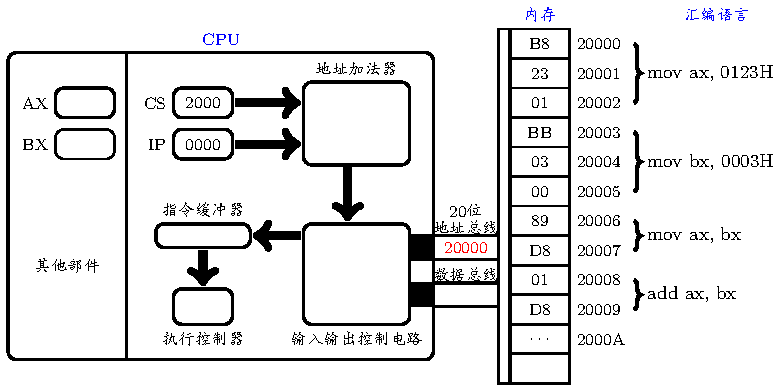
\includegraphics[width=4.5in]{Tikz/csip4}
%\caption{输入输出控制电路将物理地址送上地址总线}
%\end{figure}
%
%\end{frame}
%
%\begin{frame}\ft{CS和IP}
%\begin{figure}
%\centering
%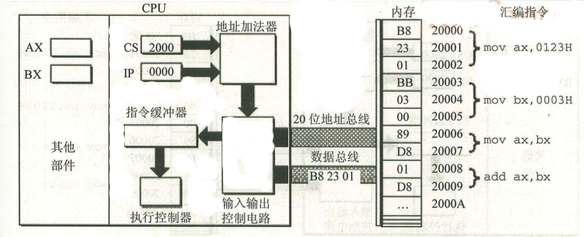
\includegraphics[width=4.5in]{Tikz/csip5}
%\caption{将内存20000H单元开始存放的机器指令B8~23~01通过数据总线送入CPU}
%\end{figure}
%
%\end{frame}
%
%
%\begin{frame}\ft{CS和IP}
%\begin{figure}
%\centering
%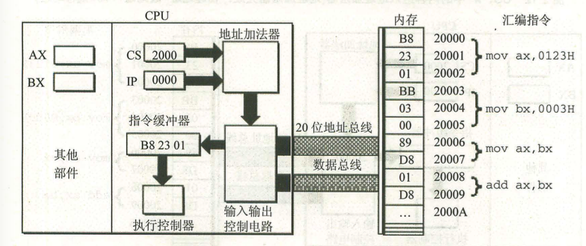
\includegraphics[width=4.5in]{Tikz/csip6}
%\caption{输入输出控制电路将机器指令B8~23~01送入指令缓冲器}
%\end{figure}
%
%\end{frame}
%
%\begin{frame}\ft{CS和IP}
%\begin{figure}
%\centering
%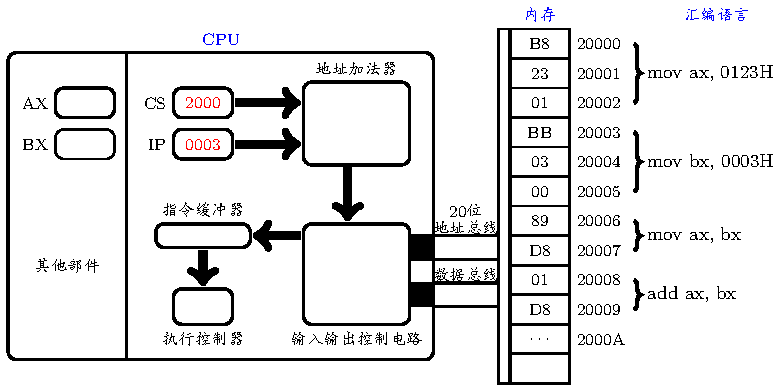
\includegraphics[width=4.5in]{Tikz/csip7}
%\caption{IP中的值自动增加:读取一条指令后,IP中的值自动增加,以使CPU可以读取下一条指令。因当前读入的指令B8~23~01为3个字节,故IP中的值加3。}
%\end{figure}
%
%\end{frame}
%
%
%\begin{frame}\ft{CS和IP}
%\begin{figure}
%\centering
%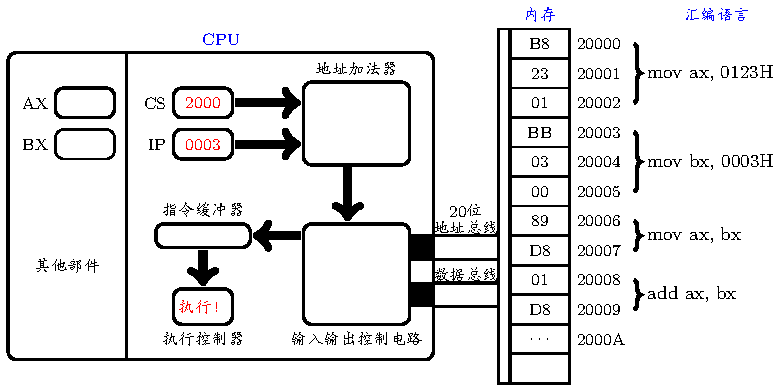
\includegraphics[width=4.5in]{Tikz/csip8}
%\caption{执行控制器执行指令B8~23~01,即mov ax, 0123H}
%\end{figure}
%
%\end{frame}
%
%\begin{frame}\ft{CS和IP}
%\begin{figure}
%\centering
%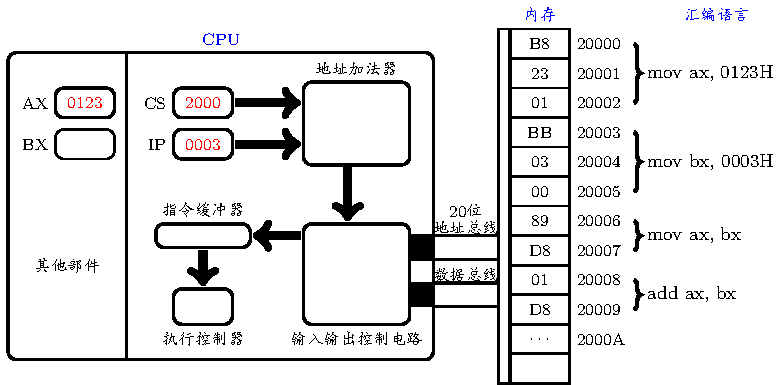
\includegraphics[width=4.5in]{Tikz/csip9}
%\caption{指令B8~23~01被执行后AX中的内容为0123H,此时CPU将从内存单元2000:0003处读取指令。}
%\end{figure}
%
%\end{frame}
%
%\begin{frame}\ft{CS和IP}
%\begin{figure}
%\centering
%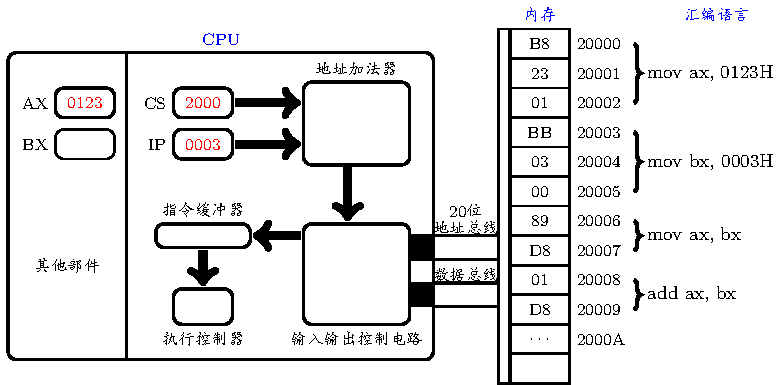
\includegraphics[width=4.5in]{Tikz/csip9}
%\caption{CS:2000H,IP:0003H,CPU将读取指令BB~03~00}
%\end{figure}
%
%\end{frame}
%
%\begin{frame}\ft{CS和IP}
%\begin{figure}
%\centering
%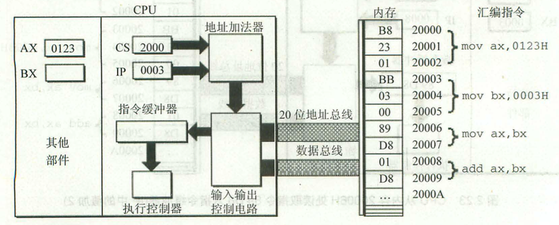
\includegraphics[width=4.5in]{Tikz/csip10}
%\caption{CPU读取指令BB~03~00入指令缓冲器,IP中的值加3。}
%\end{figure}
%
%\end{frame}
%
%
%
%
%\begin{frame}\ft{CS和IP}
%\begin{figure}
%\centering
%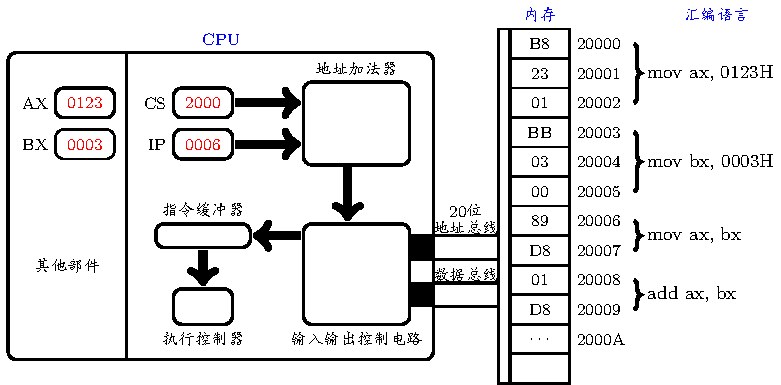
\includegraphics[width=4.5in]{Tikz/csip11}
%\caption{执行指令BB~03~00,即mov bx, 0003H}
%\end{figure}
%
%\end{frame}
%
%
%\begin{frame}\ft{CS和IP}
%\begin{figure}
%\centering
%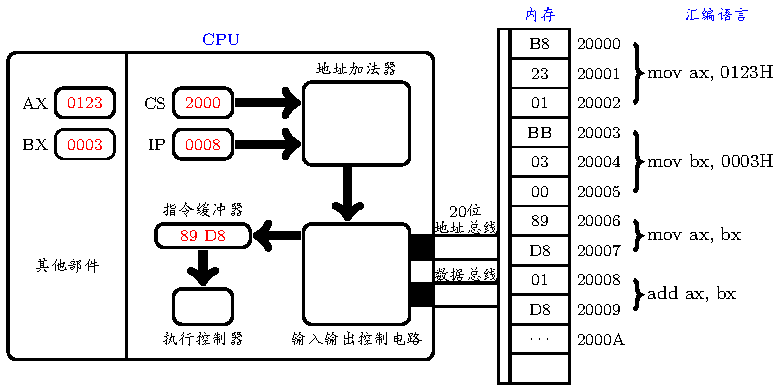
\includegraphics[width=4.5in]{Tikz/csip12}
%\caption{CPU从内存20006H处读取指令89~D8如指令缓冲器,IP中的值加2。}
%\end{figure}
%
%\end{frame}
%
%\begin{frame}\ft{CS和IP}
%\begin{figure}
%\centering
%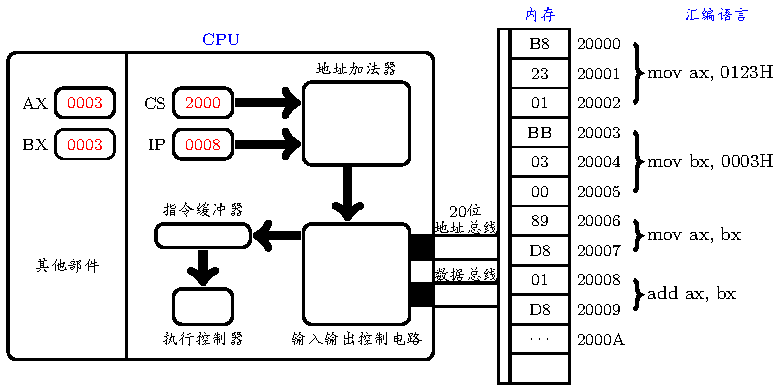
\includegraphics[width=4.5in]{Tikz/csip13}
%\caption{执行指令89~D8,即mov ax, bx后,AX中的内容为0003H}
%\end{figure}
%
%\end{frame}
%
%\begin{frame}\ft{CS和IP}
%\begin{figure}
%\centering
%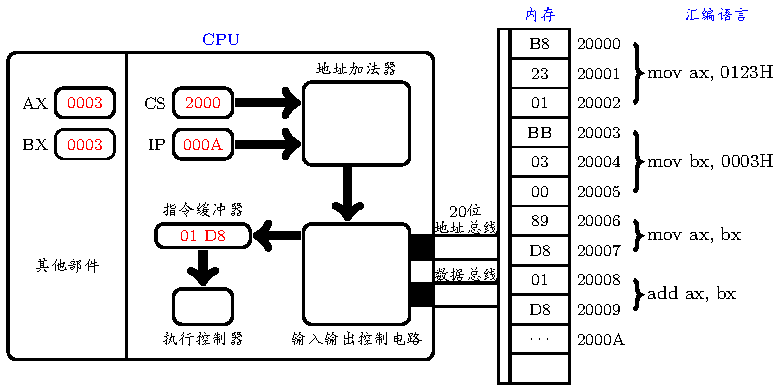
\includegraphics[width=4.5in]{Tikz/csip14}
%\caption{CPU从内存20008H处读取指令01~D8如指令缓冲器,IP中的值加2。}
%\end{figure}
%
%\end{frame}
%
%\begin{frame}\ft{CS和IP}
%\begin{figure}
%\centering
%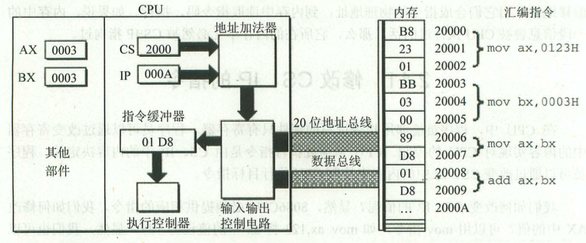
\includegraphics[width=4.5in]{Tikz/csip15}
%\caption{执行指令01~D8,即add ax, bx后,AX中的内容为0006H}
%\end{figure}
%\end{frame}
%
%\begin{frame}\ft{CS和IP}
%8086CPU的工作过程:\vspace{0.1in}
%
%\begin{itemize}
%\item[(1)] 从CS:IP指向的内存单元读取指令,读取的指令进入指令缓冲器;\\[0.1in]
%\item[(2)] IP=IP+所读取指令的长度,从而指向下一条指令;\\[0.1in]
%\item[(3)] 执行指令。转至步骤(1),重复整个过程。
%\end{itemize}
%\end{frame}
%
%\begin{frame}\ft{CS和IP}
%CPU刚开始工作时,CS和IP被设置为CS=FFFFH,IP=0000H,即开机时,CPU从内存FFFF0H单元中读取指令执行,FFFF0H单元中的指令是开机后执行的第一条指令。
%\end{frame}
%
%
%

    \section{C语言简介}


\begin{frame}\ft{C的起源}
\begin{itemize}
    \item 
      \red{产生时间:}1972-1973年\\[0.2in]
    \item 
      \red{产生地点:}美国贝尔实验室\\[0.2in]
    \item 
      \red{创始人:}Dennis Ritchie \& Ken Thompson\\[0.2in]
    \item  
      \red{目的:}改写Unix系统\\[0.2in]
    \item 
      \red{荣誉:}美国国家技术奖章(1999)
    \end{itemize}
\end{frame}



\begin{frame}\ft{C的起源}
\begin{figure}
\centering

\includegraphics[width=4in]{ch01/fig/Ritche}
\end{figure}
\end{frame}

\begin{frame}\ft{C的起源}
\begin{figure}
\centering
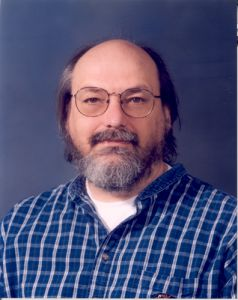
\includegraphics[width=2in]{ch01/fig/Thompson}
\caption{Ken Thompson (1942-)}
\end{figure}
\end{frame}

\begin{frame}\ft{C的起源}
\begin{figure}
\centering
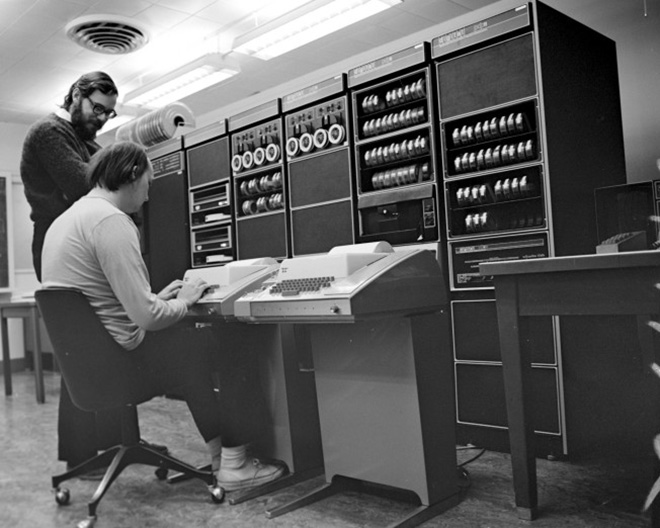
\includegraphics[width=3in]{ch01/fig/Ritche_Thompson}
\caption{Dennis Ritchie和Ken Thompson(1972年)}
\end{figure}
\end{frame}

\begin{frame}\ft{C的起源}
1983年,Dennis Ritchie和Ken Thompson一起获得了图灵奖,理由是:“研究发展了通用的操作系统理论,尤其是实现了Unix操作系统”。
\end{frame}

\begin{frame}\ft{关于Ritche的评价}
\begin{figure}
\centering
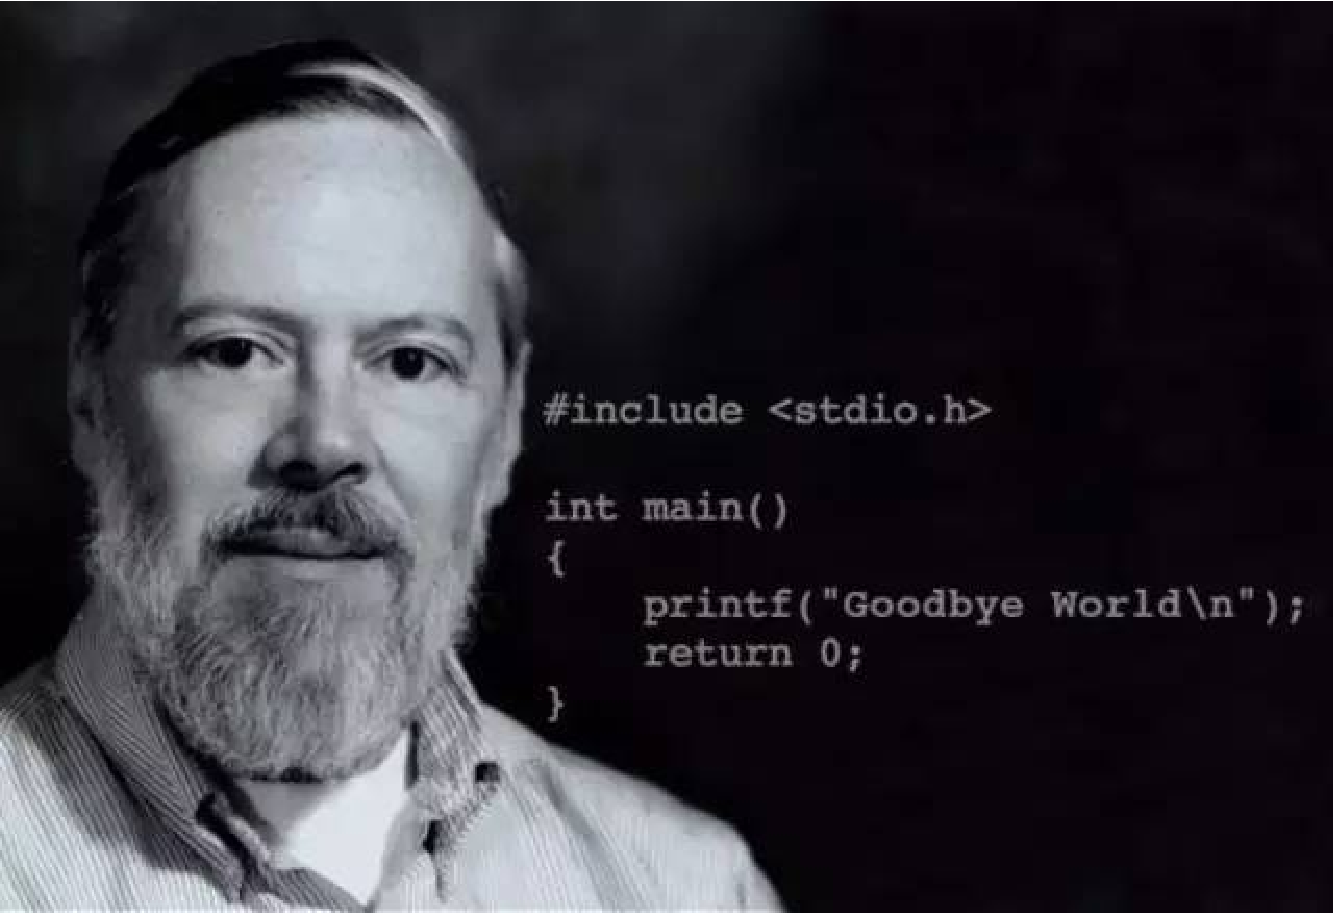
\includegraphics[width=3.5in]{ch01/fig/Ritche1}
\end{figure}

\end{frame}

\begin{frame}\ft{关于Ritche的评价1}

“当乔布斯去世时,享受到了声势浩大的追思。相形之下,里奇先生对当代科技进程做出了更大的贡献,可公众甚至不知道他是谁,这十分不公平。” 
\end{frame}

\begin{frame}\ft{关于Ritche的评价2}
“如果说,乔布斯是可视化产品中的国王,那么里奇就是不可见王国中的君主。乔布斯的贡献在于,他如此了解用户的需求和渴求,以至于创造出了让当代人乐不思蜀的科技产品。然而,却是里奇先生为这些产品提供了最核心的部件,人们看不到这些部件,却每天都在使用着。”
\end{frame}

\begin{frame}\ft{关于Ritche的评价3}
\red{“牛顿说他是站在巨人的肩膀上,如今,我们都站在里奇的肩膀上。”}

\end{frame}


\begin{frame}\ft{C的地位}
\begin{itemize}
\item  C拥有汇编语言的力量和便利性,其运行方式更接近于硬件系统;\vskip.1in
\item  C所提供的数据结构,力发千钧,足以贯穿所有高层和底层的语言;
\end{itemize}

\end{frame}

\begin{frame}\ft{C的地位}
\begin{itemize}
\item
C的开发是科技史上不可磨灭的伟大贡献,因为这个语言把握住了计算机科技中一个至关重要的并且是恰到好处的中间点,一方面它具备搭建高层产品的能力,另一方面又能够对于底层数据进行有效控制。正是由于这种关联性和枢纽性作用,决定了 C所导向的近三十年来计算机编程主流方式。
\end{itemize}

\end{frame}

\begin{frame}\ft{C的优点}
\begin{itemize}
\item[(1)] \red{设计特性}\quad 融合了控制特性,使得用户可以采用自顶而下的结构化编程,以及模块化的设计,从而使编写出的程序更可靠、更易懂 \\[0.1in] 
 
\item[(2)] \red{高效性}\quad  代码紧凑且运行速度快,可以表现出只有汇编语言才具有的精细控制能力  \\[0.1in] 
 
\item[(3)] \red{可移植性}\quad 在一个系统上编写的程序经过很少改动或不经修改就可以在其他系统上运行 \\[0.1in] 
 
\item[(4)] \red{强大的功能与灵活性}\\[0.1in] 
\begin{itemize}
\item  强大而灵活的UNIX操作系统便是用C编写的   \\[0.1in] 
\item  其他语言(如Fortran、Python等)的许多编译器和解释器都是用C编写的\\[0.1in] 
\end{itemize}

\item[(5)] \red{面向程序员}\\[0.1in] 
\begin{itemize}
\item 允许你访问硬件,并可以操纵内存中的特定位  \\[0.1in] 
\item 具有丰富的运算符供选择,让你能够简洁地表达自己的意图 
\end{itemize}
\end{itemize}

\end{frame}

\begin{frame}\ft{C的缺点}
\begin{itemize}
\item[(1)]  在表达方面的自由会增加风险。\\[0.1in]
\item[(2)]  对指针的使用,可能导致你会犯难以追踪的编程错误。\\[0.1in]
\item[] \red{自由的代价是永远的警惕。}\\[0.2in]
\item[(3)]  其简洁性与丰富的运算符相结合,可能会产生极难理解的代码。\\[0.1in]
\item[]  \red{含糊代码竞赛}
\url{www.ioccc.org}
\end{itemize}
\end{frame}

    \section{使用C语言的七个步骤}

 

\begin{frame}\ft{\secname}
  
\begin{enumerate}
\item  定义程序目标\\[0.1in]
%\item[] 开始时应对程序做什么有一个清晰的想法。\\[0.1in]
%\item[] 考虑程序需要的信息、需要进行的计算和操作,以及程序应该向你报告的信息。
 
\item  设计程序\\[0.1in]
%\item[] 如何表示数据   \\[0.1in]
%\item[] 用什么方法处理数据  \\[0.1in]
%\item[] \red{选择一个好的方式来表示信息可以使程序设计和数据处理容易很多}
 
\item  编写代码\\[0.1in]
%\item[] 用文本编辑器创建一种称为源代码的文件。
%\item[] 常见的文本编辑器Ultraedit、Emacs、Vi、集成开发环境(IDE)中自带的编辑器等。
% 
\item  编译 \\[0.1in]
%\item[] 编译器将源代码转换为可执行文件,可执行文件是机器语言表示代码。\\[0.2in]
\item 运行程序 \\[0.1in]
%\item[] 在Dos、Unix和Linux系统中,可在命令行中直接键入可执行文件名即可运行程序。\\[0.1in]
%\item[] 在Windows和MAC环境提供的IDE中可通过选择菜单选项或特定快捷键来执行程序。 
% 
\item  测试和调试程序\\[0.1in]
%\item[] Bug\\[0.1in]
%\item[] Debug\\[0.2in]

\item   维护和修改程序\\[0.1in]
\end{enumerate} 
 
\end{frame}




    \section{编译C程序的工作原理}
\begin{frame}\ft{\secname}
C是一种高级语言,它需要编译器将其转换为可执行代码,以使得程序能在机器上运行。 

以下介绍在MAC或Linux上使用gcc编译器的几个步骤。

\end{frame}


\begin{frame}[fragile]\ft{\secname}
\begin{itemize}

\item[(1)] 用编辑器(vi,emacs等)创建一个C程序,并将其保存为 \lstinline|add2num.c|。

\begin{lstlisting}
$ emacs add2num.c
\end{lstlisting} 

\pause 
\lstinputlisting[]{ch01/code/add2num.c}

\end{itemize}
\end{frame}

\begin{frame}[fragile]\ft{\secname}
\begin{itemize}
\item[(2)] 编译 
\begin{lstlisting}
$ gcc -wall add2num.c –o add2num
$ ls
add2num    add2num.c
\end{lstlisting}
\begin{itemize}
	\item \lstinline|-Wall| \quad 启动所有编译器的警告信息。建议使用该选项以生成更好的代码 \\[.1in]
	\item \lstinline|-o| \quad 指定可执行文件名。若缺省,则可执行文件名将默认为\lstinline|a.out|
\end{itemize} 
\end{itemize}
\end{frame}

\begin{frame}[fragile]\ft{\secname}
\begin{itemize}
\item[(3)] 运行可执行文件。


\begin{lstlisting}
$ ./add2num
Addition is: 9
\end{lstlisting}

\end{itemize}
\end{frame}



\begin{frame}[fragile]\ft{\secname}
编译器将一个C程序转换为一个可执行文件,需经历了4个阶段:
\begin{itemize}
\item 预处理\\[.1in]
\item 编译\\[.1in]
\item 汇编\\[.1in]
\item 链接
\end{itemize}
\end{frame}


\begin{frame}[fragile]\ft{\secname}
执行以下命令,在当前目录下会生成所有的中间文件以及可执行文件。
\begin{lstlisting}
$ gcc -Wall -save-temps filename.c –o filename 
$ ls 
add2num     add2num.c   add2num.o
add2num.bc  add2num.i   add2num.s
\end{lstlisting}

接下来,让我们一个个地来看这些中间文件中的内容。 
\end{frame}


\begin{frame}[fragile]\ft{\secname}

\begin{itemize}
\item[(1)] \blue{预处理} \quad 其输出保存在文件 \lstinline|add2num.i| 中。\\[.1in]

\begin{itemize}
\item 去掉注释\\[.1in]
\item 宏的展开\\[.1in]
\item 头文件的展开\\[.1in]
\end{itemize}
 
\end{itemize}
\pause 

\begin{lstlisting}
$ less add2num.i
$ ls 
...
int printf(const char * restrict, ...) __attribute__((__format__ (__printf__, 1, 2)));
# 499 "/usr/include/stdio.h" 2 3 4
# 3 "add2num.c" 2

int main(void)
{
  int a = 5, b = 4;
  printf("Addition is: %d\n", (a+b));
  return 0;
}
\end{lstlisting}
\end{frame}


%\begin{frame}[fragile]\ft{\secname}
%\red{分析:}在以上内容中,源文件被附加了很多信息,但在末尾代码仍被保留。{\ttfamily printf()}函数中包含了{\ttfamily a+b}而非{\ttfamily add(a,b)},因为宏已被展开。注释被去除掉。{\ttfamily\#include<stdio.h>}没有了,取而代之的是很多代码。因此,头文件已被展开,并且被包含到了源文件中。
%
%\end{frame}


\begin{frame}[fragile]\ft{\secname}
\begin{itemize}
\item[(2)] \blue{编译} \quad  编译 \lstinline|add2num.i|,生成文件 \lstinline|add2num.s| 。该文件为汇编指令,可用以下命令查看:
\end{itemize} 
\begin{lstlisting}
$ less add2num.s
...
        movl    $0, -4(%rbp)
        movl    $5, -8(%rbp)
        movl    $4, -12(%rbp)
        movl    -8(%rbp), %eax
        addl    -12(%rbp), %eax
        movl    %eax, %esi
        movb    $0, %al
        callq   _printf
        xorl    %esi, %esi
...      
\end{lstlisting}
\end{frame}


\begin{frame}[fragile]\ft{\secname}
\begin{itemize}
\item[(3)] \blue{汇编} \quad 通过汇编器将 \lstinline|add2num.s| 转换成 \lstinline|add2num.o|,该文件包含机器指令。\\[.1in]
\begin{itemize}
	\item  该阶段只会将现有代码转换成机器语言,而诸如 \lstinline|printf()| 的函数调用则不会。
\end{itemize}
\end{itemize}
\pause 
\begin{lstlisting}
$ less add2num.o
<CF><FA><ED><FE>^G^@^@^A^C^@^@^@^A^@^@^@^D^@^@^@^@^B^@^@^@ ^@^@^@^@^@^@^Y^@^@^@<88>^A^@^@^@^@^@^@^@^
...      
\end{lstlisting}

\end{frame}


\begin{frame}[fragile]\ft{\secname}
\begin{itemize}
\item[(4)] \blue{连接} \quad 完成所有函数调用及其定义的连接工作。\\[.1in]

\begin{itemize}
	\item 链接器知道所有这些函数在何处执行 \\[.1in]
	\item 链接器也会做一些额外的工作,以添加一些启动和结束程序所需的额外代码 \\[.1in]
\end{itemize} 
\end{itemize}
\pause 


%在命令行中输入以下命令,可看出从目标文件到可执行文件时文件大小的变化。这是因为链接器为我们的程序添加了额外的代码。
\begin{lstlisting}
$ size add2num.o
__TEXT  __DATA  __OBJC  others    dec         hex
  145     0       0       32      177         b1	
  
$ size add2num
__TEXT  __DATA  __OBJC  others    dec         hex
4096      4096    0  4294971392 4294979584 100003000
\end{lstlisting}

\end{frame}

  }{}
  \ifthenelse{\equal{#1}{s2}}{
    \section{简单实例}
%\lstset{frameshape={RYRYNYYYY}{yny}{yny}{RYRYNYYYY}}

\begin{frame}\ft{\subsecname}
  \lstinputlisting[
    language=c,
    frame=single,
    numbers=left
  ]{ch02/code/first.c}
\end{frame}








    \section{程序解释}
\begin{frame}\ft{\lstinline|\#include|与头文件}

\lstinputlisting[
language=c,
linerange={2-2},
firstnumber=2,
numbers=left,
]{ch02/code/first.c}

\begin{itemize}
\item
相当于在此处复制文件\lstinline|stdio.h|的完整内容,以方便在多个程序间共享公用信息。\\[0.1in]
\item
\lstinline|\#include|语句是C预处理器指令的一个例子。通常,C编译器在编译前要对源代码做一些准备工作,这称为预处理。
\\[0.1in]
\item
文件\lstinline|stdio.h|包含了有关输入和输出函数的信息,以供编译器使用。
\end{itemize}
\end{frame}

\begin{frame}\ft{\lstinline|main| 函数}
\lstinputlisting[
language=c,
linerange={3-3},
firstnumber=3,
numbers=left,
frame=none
]{ch02/code/first.c}
 
C程序至少包含一个函数,函数是C程序的基本模块。\\[0.1in]
\begin{table}
\centering
\begin{tabular}{ll}
表达式 & 含义 \\ \hline
\lstinline|( )| &  函数名为 \lstinline|main| \\[0.1in]
\lstinline|int| &  返回一整数\\[0.1in]
\lstinline|void| & 不接受任何参数 \\ \hline
\end{tabular}
\end{table}
 
注:\lstinline|main| 函数是任何C程序的唯一入口。
\end{frame}

\begin{frame}[fragile]\ft{\lstinline|main| 函数}
\lstinline|main| 函数有三种定义:
\begin{lstlisting}
// Definition 1: NOT RECOMMENDED
void main() { /* ... */ }

// Definition 2
int main() { /* ... */ }

// Definition 3
int main(int argc, char* argv[]) { /* ... */ }
\end{lstlisting}
\end{frame}

\begin{frame}[fragile]\ft{\lstinline|main| 函数}
考虑\lstinline|main| 函数的两种定义,它们的差别是什么?
\begin{lstlisting}
int main()
{
   /*  */
   return 0;
}

int main(void)
{
   /*  */
   return 0;
}
\end{lstlisting}
\pause
\begin{itemize}
\item 在C++中,两种没有差别,完全一致。
\item 在C中,两种定义都可以,但是第二种定义更好,因它清晰地表明main()在调用时不允许有参量。	
\end{itemize}
\end{frame}

\begin{frame}[fragile]\ft{\lstinline|main| 函数}
在C中,如果一个函数没有指定任何参量,就意味着该函数允许在调用时有任意多个参量或者无参量。
 
\begin{lstlisting}
// Program 1 (Compiles and runs fine in C, but not in C++)
void fun() {  } 
int main(void)
{
    fun(10, "GfG", "GQ");
    return 0;
}
\end{lstlisting}
上述程序能编译和运行,但以下程序编译会失败。
 
\begin{lstlisting}
// Program 2 (Fails in compilation in both C and C++)
void fun(void) {  }
int main(void)
{
    fun(10, "GfG", "GQ");
    return 0;
}
\end{lstlisting}
\end{frame}

\begin{frame}[fragile]\ft{\lstinline|main| 函数}

\begin{itemize}
\item 在C++中,以上两个程序在编译时都会失败,因为在C++中,\lstinline|fun()| 和 \lstinline|fun(void)| 无差别。\\[.1in]
\item 在C中, \lstinline|int main()| 和 \lstinline|int main(void)|的差别在于,前者允许在调用时有任意多个参量,而后者在调用时不能有任何参量。\red{尽管两者在大多数时候无任何差别,但在实践中更推荐使用 \lstinline|int main(void)|。}
\end{itemize}

\end{frame}

\begin{frame}[fragile]\ft{\lstinline|main| 函数}
以下C程序的输出是什么?
\lstinputlisting[]{ch02/code/question1.c}
 
\lstinputlisting[]{ch02/code/question2.c}

\end{frame}

\begin{frame}\ft{注释}
 
\lstinputlisting[
language=c,
linerange={4-4},
firstnumber=4,
numbers=left,
frame=none
]{ch02/code/first.c}
 


\begin{overprint}
\begin{itemize}
\item \lstinline|/* ... */| 之间的内容是程序注释。\\[0.1in]
\item 注释可以让阅读者更容易理解程序。\\[0.1in]
\item 注释可以放在任意位置,甚至和它要解释的语句在同一行。\\[0.1in]
\item 一个较长的注释可以单独放一行,也可以是多行。\\[0.1in]
\item \lstinline|/* ... */| 之间的所有内容都会被编译器忽略。
\end{itemize}
\end{overprint}

\end{frame}

\begin{frame}[fragile]\ft{注释}
\begin{lstlisting}[language=c]
/* This is a C comment.*/

/* This comment is spread over
   two lines. */

/*
   You can do this, too.
*/

/* invalid comment
\end{lstlisting}
\end{frame}

\begin{frame}[fragile]\ft{注释}
C99增加另一种风格的注释,使用 \lstinline|//| 符号,该风格在C++和Java中经常使用。 \vspace{0.2in}


\begin{lstlisting}[language=c]
// Here is a comment confined to one line

int n; // Such comments can go here, too.
\end{lstlisting}
\end{frame}

\begin{frame}[fragile]\ft{花括号,程序体和代码块}
 
\begin{lstlisting}[language=c,frame=none]
{
  ...
}
\end{lstlisting}
 
\begin{itemize}
\item
C函数使用花括号表示函数体的开始和结束。\\[0.2in]
\item
花括号还可以用来把函数中的语句聚集到一个单元或代码块中。
\end{itemize}
\end{frame}

\begin{frame}[fragile]\ft{声明}
\lstinputlisting[
language=c,
linerange={6-6},
firstnumber=6,
numbers=left,
frame=none
]{ch02/code/first.c}

 
声明语句(declaration statement),做两件事情:\vspace{0.1in}
\begin{itemize}
\item 
在内存中为变量 \lstinline|num| 分配了空间。\\[0.1in]
\item 
 \lstinline|int| 说明变量 \lstinline|num| 的类型(整型)。
\end{itemize} \vspace{0.1in}

\pause 

注意:分号指明该行是C的一个语句。分号是语句的一部分。
 
\end{frame}

\begin{frame}[fragile]\ft{声明}
Ansi C要求必须在一个代码块的开始处声明变量,在这之前不允许其他任何语句。

\begin{lstlisting}[
language=c,
numbers=left,
frame=none
]
int main(void)
{
  int n;
  int m;
  n = 5;
  m = 3;
  // other statements
}
\end{lstlisting}
\end{frame}

\begin{frame}[fragile]\ft{声明}
C99遵循C++的惯例,允许把声明放在代码块的任何位置。但是在首次使用变量之前仍必须先声明它。

\begin{lstlisting}[
language=c,
numbers=left,
frame=none
]
int main(void)
{
  int n;
  n = 5;
  // more statements
  int m;
  m = 3;
  // other statements
}
\end{lstlisting}
\end{frame}


\begin{frame}[fragile]\ft{声明}
\begin{wenti}
\begin{itemize}
\item 什么是数据类型?\\[.1in]
\item 怎么给变量取名? \\[.1in]
\item 为什么必须对变量进行声明?
\end{itemize}
\end{wenti}
\end{frame}

\begin{frame}[fragile]\ft{声明}
\begin{enumerate}[1]
\item \red{数据类型}\\[0.1in]
\begin{itemize}
\item   C可以处理多个数据种类,如整数、字符和浮点数。\\[0.1in]
\item   把一个变量声明为整数类型、字符类型或浮点数类型,是计算机能正确存储、获取和解释该数据的基本前提。
\end{itemize}

\item \red{取名}\\[0.1in]
\begin{itemize}
\item  “见其名只其意”。\\[0.1in]
\item  若名字不能表达清楚,可以用注释解释变量所代表的意思。\\[0.1in]
\end{itemize}

\item \red{命名规则:} \\[0.1in]
\begin{itemize}
\item 只能使用\red{字母、数字和下划线},且第一个字符不能为数字。 \\[0.1in]
\item 操作系统和C库通常使用以一个或两个下划线开始的名字,因此最好避免这种用法。 \\[0.1in]
\item \red{区分大小写},如stars不同于Stars或STARS。
\end{itemize}
\end{enumerate}

\end{frame}


\begin{frame}[fragile]\ft{声明}

\begin{table}
\centering
\caption{正确和错误的名字}
\begin{tabular}{c|c}\hline
${\checkmark}$&${\times}$\\[0.1in]\hline
\lstinline|wiggles |&   \lstinline|$zj**|\\[0.1in]
\lstinline|cat2| &  \lstinline|2cat|\\[0.1in]
\lstinline|Hot_Dog| &  \lstinline|Hot-Dog|\\[0.1in]
\lstinline|taxRate| &  \lstinline|tax Rate|\\[0.1in]
\lstinline|_kcab| &  \lstinline|don't|\\\hline
\end{tabular}
\end{table}


\end{frame}


\begin{frame}[fragile]\ft{声明变量的好处}
\begin{itemize} 
\item 把所有变量放在一起,可以让读者更容易掌握程序的内容。
\\[0.1in]
\item  在开始编写程序之前,考虑一下需要声明的变量会促使你做一些计划。\\[0.1in]
\item  声明变量可以帮助避免程序中出现一类很难发现的细微错误,即变量名的错误拼写。\\[0.1in]
\item  所有变量都需要声明,否则程序将不能编译。
\end{itemize}
\end{frame}


\begin{frame}[fragile]\ft{赋值}
\lstinputlisting[
language=c,
linerange={7-7},
firstnumber=7,
numbers=left,
frame=none
]{ch02/code/first.c}

 
这是一条赋值语句(Assignment statement),其含义:把值 \lstinline|1| 赋给变量 \lstinline|num|。
 
\end{frame}


\begin{frame}[fragile]\ft{\lstinline|printf| 函数}
\lstinputlisting[
language=c,
linerange={8-10},
firstnumber=8,
numbers=left,
frame=none
]{ch02/code/first.c}
 

\lstinline|printf| 是一个标准输出函数,其信息由头文件 \lstinline|stdio.h| 指定。
%\vspace{0.1in}
%
%圆括号表明printf为函数名,圆括号内为参数(argument)。这里的参数都是字符串,即双引号之间的内容。
% 
\end{frame}


\begin{frame}[fragile]\ft{转义字符}
 
\red{转义字符}通常用于代表难以表达或无法键入的字符,以 \lstinline|\| 开头。
 
\begin{table}
\centering
\begin{tabular}{c|c} \hline
转义字符 & 含义 \\[.1in] \hline  
\lstinline|\n| & 换行\\[.1in]
\lstinline|\t| & Tab键\\[.1in]
\lstinline|\b| & 退格\\[.1in]
\lstinline|\'| & 单引号\\[.1in]
\lstinline|\"| & 双引号\\[.1in]
$\backslash\backslash$ & 反斜杠\\[.1in]
\hline 
\end{tabular}
\end{table}
\end{frame}


\begin{frame}[fragile]\ft{格式化字符串}
\red{格式化字符串},也称\red{占位符},用以指定输出项的数据类型和输出格式,以 \lstinline|%| 开头。

\begin{table}
\centering
\begin{tabular}{c|c}\hline
占位符 & 含义 \\ \hline  
\lstinline|%d| & 用于输出十进制整数(实际长度)\\[0.1in]
\lstinline|%c| & 输出一个字符\\[0.1in]
\lstinline|%s| & 输出一个字符串\\[0.1in]
\lstinline|%f| & 以小数形式输出实数(整数部分全部输出,小数部分6位)\\
\hline 
\end{tabular}
\end{table}
 
\end{frame}

\begin{frame}[fragile]\ft{\lstinline|return|语句}
\lstinputlisting[
language=c,
linerange={11-11},
firstnumber=11,
numbers=left,
frame=none
]{ch02/code/first.c}

带有返回值的C函数要求使用一个\lstinline|return|语句,该语句包含关键字\lstinline|return|,后面紧跟要返回的值。

\end{frame}

    \section{使程序可读的技巧}
\begin{frame}[fragile]\ft{\secname}
\begin{itemize}
\item 变量命名时做到“见其名知其意”;\\[0.1in]
\item 合理使用注释;\\[0.1in]
\item 使用空行分隔一个函数的各个部分,如声明、操作等;\\[0.1in]
\item 每条语句用一行。注意,C允许把多条语句放在同一行或一条语句放多行。
\end{itemize}
\end{frame}


\begin{frame}[fragile]\ft{\secname}
\lstinputlisting[language=c]{ch02/code/mile_km.c}
\end{frame}


\begin{frame}[fragile]\ft{\secname}
\begin{itemize}
	\item 建议在程序开始处,用一个注释说明文件名和程序的作用,这对以后浏览或打印程序很有帮助。\\[0.1in]
	\item 多个声明 \\[0.1in]
	
\begin{minipage}{.4\textwidth}
\begin{lstlisting}[language=c]
float mile, km;
\end{lstlisting}
\end{minipage}	$~~\Leftrightarrow~~$
\begin{minipage}{.4\textwidth}
\begin{lstlisting}[language=c]
float mile;
float km;
\end{lstlisting}
\end{minipage}

\item 输出多个值

\begin{itemize}
	\item 第一个printf语句用了两个占位符:第一个\%d为mile占位,第二个\%d为km占位;圆括号中有三个参数,之间用逗号隔开。\vspace{0.1in}
	\item 
	第二个printf语句说明输出的值可以是一个表达式。
\end{itemize}

\end{itemize}
 

\end{frame}
 
    \section{多个函数}
\begin{frame}[fragile]\ft{\secname}
  当程序比较复杂时,使用多个函数会可实现程序的模块化,使程序可读性更强。
\end{frame}

\begin{frame}\ft{\secname}
\lstinputlisting{ch02/code/mile2km.c}
\end{frame}

\begin{frame}[fragile]\ft{\secname}
\lstinline|mile2km()| 函数出现了三次:\vspace{0.1in}

\begin{enumerate}
\item 函数声明:通知编译器要用到该函数。\\[0.1in]
\item 函数调用\\[0.1in]
\item 函数定义
\end{enumerate}
\end{frame}

    \section{调试}
\begin{frame}[fragile]\ft{调试}
找出以下程序中的错误。
\begin{lstlisting}[language=c,numbers=left,frame=tb]
#include<stdio.h>
int main(void) 
(
  int n, int n2, int n3;
  /* `该程序含几个错误`    
  n = 5; n2 = n * n;
  n3 = n2 * n2;
  printf("n = %d, n^2 = %d, n^3 = %d\n", n, n2, n3)	 
  return 0;
)
\end{lstlisting}
\end{frame}

\begin{frame}[fragile]\ft{语法错误}
\begin{dingyi}[语法错误] 
把正确的C符号放在了错误的位置。
\end{dingyi}\pause 

\begin{enumerate}
\item 使用圆括号而不是花括号来包围函数体。\\[0.1in]
\item 声明方式应采用

\begin{minipage}{0.4\linewidth}
\begin{lstlisting}[language=c,frame=single]
int n, n2, n3;
\end{lstlisting}
\end{minipage}
~~~~或~~~~
\begin{minipage}{0.4\linewidth}
\begin{lstlisting}[language=c,frame=single]
int n;
int n2;
int n3;
\end{lstlisting}
\end{minipage}
\item 注释应该用 “\lstinline|/* ... */|” 或 “\lstinline|// ...|” 的形式。\\[0.1in]
\item \lstinline|printf|语句最后漏掉了分号。
\end{enumerate}
\end{frame}

\begin{frame}[fragile]\ft{语法错误}
\begin{wenti}
如何检测语法错误?
\end{wenti}\pause 

\begin{enumerate}
\item 在编译前看看源代码是否有明显的错误。\\[0.1in]
\item 查看编译器发现的错误。若有语法错误,编译时会报错,同时指出每一个错误的性质和位置。
\end{enumerate}

\end{frame}


\begin{frame}[fragile]\ft{语义错误}
\begin{dingyi}[语义错误]
逻辑或含义上的错误。当语法没有错误,但结果不正确时,就是犯了语义错误。
\end{dingyi}\pause  \vspace{.1in}


\begin{lstlisting}[language=c,frame=tb]
n3 = n2 * n2;
\end{lstlisting}
本希望 \lstinline|n3| 表示 \lstinline|n| 的三次方,但求的却是 \lstinline|n| 的四次方。\pause \vspace{0.1in}


语义错误编译器检测不到,它并没违法C规则。但编译器无法了解你的真正意图,只能靠你自己去发现这类错误。

\vspace{.1in}\pause 

\blue{语义错误可以通过调试器来一步一步执行程序,来逐步跟踪和定位。}
\end{frame}


    \section{关键字}
\begin{frame}[fragile]\ft{\secname}
关键字是C中的特殊词汇,不能用它们来对变量或者函数命名。
若试图把一个关键字作为变量名,编译器把它当做一个语法错误。
\end{frame}

\lstset{language=[ansi]c}
\begin{frame}[fragile]\ft{\secname}
\begin{table}
\centering
\caption{C关键字}
\begin{tabular}{p{2cm}p{2cm}p{2cm}p{2cm}}\hline
\lstinline|auto| & \lstinline|enum| & \lstinline|restrict| & \lstinline|unsigned| \\
\lstinline|break| & \lstinline|extern| & \lstinline|return| & \lstinline|void| \\
\lstinline|case| & \lstinline|float| & \lstinline|short| &\lstinline|volatile| \\
\lstinline|char| & \lstinline|for| & \lstinline|signed| & \lstinline|while| \\
\lstinline|const| & \lstinline|goto| & \lstinline|sizeof| & \lstinline|_Bool| \\
\lstinline|continue| & \lstinline|if| & \lstinline|static| & \lstinline|_Complex| \\
\lstinline|default| & \lstinline|inline| & \lstinline|struct| & \lstinline|_Imaginary|\\
\lstinline|do| & \lstinline|int| & \lstinline|switch| &  \\
\lstinline|double| & \lstinline|long| & \lstinline|typedef| & \\
\lstinline|else| & \lstinline|register| & \lstinline|union| \\ \hline
\end{tabular}
\end{table}
\end{frame}


\lstset{language=c++}
\begin{frame}[fragile]\ft{\secname}
\begin{table}
	\centering
	\caption{C++关键字}
	\begin{tabular}{p{2cm}p{2cm}p{2.5cm}p{2cm}}\hline
          \lstinline|asm|         & \lstinline|else|     & \lstinline|new|             & \lstinline|this|     \\
          \lstinline|auto|        & \lstinline|enum|     & \lstinline|operator|        & \lstinline|throw|    \\
          \lstinline|bool|        & \lstinline|explicit| & \lstinline|private|         & \lstinline|true|     \\
          \lstinline|break|       & \lstinline|export|   & \lstinline|protected|       & \lstinline|try|      \\
          \lstinline|case|        & \lstinline|extern|   & \lstinline|public|          & \lstinline|typedef|  \\
          \lstinline|catch|       & \lstinline|false|    & \lstinline|register|        & \lstinline|typeid|   \\
          \lstinline|char|        & \lstinline|float|    & \lstinline|reinterpret_cast|& \lstinline|typename| \\
          \lstinline|class|       & \lstinline|for|      & \lstinline|return|          & \lstinline|union|    \\
          \lstinline|const|       & \lstinline|friend|   & \lstinline|short|           & \lstinline|unsigned| \\
          \lstinline|const_cast|  & \lstinline|goto|     & \lstinline|signed|          & \lstinline|using|    \\  
          \lstinline|continue|    & \lstinline|if|       & \lstinline|sizeof|          & \lstinline|virtual|  \\  
          \lstinline|default|     & \lstinline|inline|   & \lstinline|static|          & \lstinline|void|     \\  		
          \lstinline|delete|      & \lstinline|int|      & \lstinline|static_cast|     & \lstinline|volatile| \\ 
          \lstinline|do|          & \lstinline|long|     & \lstinline|struct|          & \lstinline|wchar_t|  \\
          \lstinline|double|      & \lstinline|mutable|  & \lstinline|switch|          & \lstinline|while|    \\
          \lstinline|dynamic_cast|& \lstinline|namespace|& \lstinline|template|        &                      \\\hline		
        \end{tabular}
\end{table}
\end{frame}










  }{}
  \ifthenelse{\equal{#1}{s3}}{
    \section{例子}

\begin{frame}[fragile]\ft{\secname}
  编制程序,实现华氏温度到摄氏温度的转换。转化公式为
  $$
  C = \frac59 (F-32).
  $$
  其中$F$表示华氏温度,$C$表示摄氏温度。
\end{frame}

\begin{frame}[fragile]\ft{\secname}

\lstinputlisting[language=C,numbers=left,frame=single]{ch03/code/fah2cel.c}
\end{frame}

\begin{frame}[fragile]\ft{\secname}

\begin{lstlisting}
$ gcc fah2cel.c 
$ ./a.out
Please input the Fahrenheit temperature:
78
78.00 F = 25.56 C
\end{lstlisting}
\end{frame}


\begin{frame}[fragile]\ft{\secname}
\begin{itemize}
\item 
\begin{lstlisting}
float fah, cel;
\end{lstlisting}
声明两个\lstinline|float|变量\lstinline|fah, cel|。\\[0.1in]
\item \lstinline|%f|用于输出浮点型数据;\lstinline|%.2f|可以精确控制输出格式,使浮点数显示到小数点后两位。\\[0.1in]
\item 使用\lstinline|scanf()|为程序提供键盘输入。\\[0.1in]
\item[] \lstinline|%f|指示\lstinline|scanf()|从键盘读取一个浮点数;\\[0.1in]
\item[] \lstinline|&fah|表示变量\lstinline|fah|的位置,指定将输入值赋给变量\lstinline|fah|。

\end{itemize}
\end{frame}


\begin{frame}[fragile]\ft{\secname}
\begin{itemize}
\item
该程序的最大特点是\red{交互性},交互性使得程序更加灵活。\\[0.1in]
\item[] 例如,该程序可以输入任意的华氏温度,而不必每次重写。\\[0.2in]
\item \lstinline|scanf()|和\lstinline|printf()|使得这种交互成为可能。\\[0.1in]
\item[] \lstinline|scanf()|从键盘读取数据并将其传递给程序;\\[0.1in]
\item[] \lstinline|printf()|则从程序读取数据并将其打印到屏幕。\\[0.1in]
\item[] 两者一起使用,就建立起了人机之间的双向通信。
\end{itemize}

\end{frame}





    \section{基本概念}

\begin{frame}\ft{常量}
\begin{dingyi}[常量]

在程序执行过程中,其值不发生改变的量称为常量。
\end{dingyi} \vspace{0.1in}

常量分为两类:\vspace{0.05in}

\begin{enumerate}
\item 直接常量(或字面常量)\\[0.1in]
\item 符号常量
\end{enumerate}
\end{frame}


\begin{frame}\ft{直接常量}

\begin{itemize}
\item 整型常量:\lstinline|12, 0, -3|;\\[0.1in]
\item 浮点型常量:\lstinline|3.1415, -1.23|;\\[0.1in]
\item 字符型常量:\lstinline|'a', 'b'|
\end{itemize}
\end{frame}

\begin{frame}[fragile]\ft{符号常量}

\begin{dingyi}[标识符]
用来标识变量名、符号常量名、函数名、数组名、类型名、文件名的有效字符序列。
\end{dingyi} \pause \vspace{0.1in}

\begin{dingyi}[符号常量]

在C语言中,可以用一个标识符来表示一个常量,称之为符号常量。
\end{dingyi} 
\end{frame}

\begin{frame}[fragile]\ft{符号常量}
符号常量在使用之前必须先定义,其一般形式为:
\begin{lstlisting}
#define `标识符` `常量`
\end{lstlisting}
\vspace{0.05in}

\begin{itemize}
\item \lstinline|#define|是一条预处理命令,称为宏定义命令。\\[0.1in]
\item 功能是把该标识符定义为其后的常量值。\\[0.1in]
\item 一经定义,以后在程序中所有出现该标识符的地方均代之以该常量值。
\end{itemize}
\end{frame}

\begin{frame}[fragile]\ft{符号常量}
\begin{lstlisting}
#include<stdio.h>
#define PRICE 100
int main(void)
{
  int num, total;  
  num = 10;
  total = num * PRICE;
  printf("total=%d\n", total);  
  return 0;
}
\end{lstlisting}

\end{frame}

\begin{frame}[fragile]\ft{符号常量}
使用符号常量的好处是:\vspace{0.05in}

\begin{itemize}
\item 含义清楚;\\[0.1in]
\item 能做到“一改全改”。
\end{itemize}
\end{frame}


\begin{frame}\ft{变量}
\begin{dingyi}\red{变量}

在程序执行过程中,其值可以改变的量称为变量。
\end{dingyi}

\begin{itemize}
\item
一个变量应该有一个名字,在内存中占据一定的存储单元。\\[0.1in]
\item
变量定义必须放在变量使用之前。
\end{itemize}
\end{frame}


\begin{frame}\ft{变量}
\begin{itemize}
\item
一般放在函数体的开头部分。\\[0.1in]
\item
要区分变量名和变量值是两个不同的概念。
\end{itemize}

\begin{figure}
\centering
\includegraphics[width=3.5in]{ch03/images/var}
\end{figure}

\end{frame}


\begin{frame}\ft{数据类型}
\begin{figure}
\includegraphics[width=3.5in]{ch03/images/datatype}
\end{figure}
\end{frame}


\begin{frame}\ft{数据类型}
\begin{itemize}
\item 
对于常量,编译器通过书写形式来辨认其类型。\\[0.1in]
\item[] 例如,\lstinline|42|是整型,\lstinline|42.0|是浮点型。\\[0.2in]
\item
变量必须在声明语句中指定其类型。
\end{itemize}
\end{frame}

\begin{frame}\ft{数据类型关键字}
\begin{table}
\centering
\begin{tabular}{p{3cm}|p{3cm}|p{3cm}}\hline
\lstinline|int| & \lstinline|signed| & \lstinline|_Bool| \\[0.05in]
\lstinline|long| & \lstinline|void| & \lstinline|_Complex| \\[0.05in]
\lstinline|short| & & \lstinline|_Imaginary|\\[0.05in]
\lstinline|unsigned| &&\\[0.05in]
\lstinline|char| &&\\[0.05in]
\lstinline|float| &&\\[0.05in]
\lstinline|double| &&\\\hline
\end{tabular}
\end{table}
\end{frame}

\begin{frame}[fragile]\ft{数据类型关键字}
\begin{itemize}
\item 
\lstinline|int|提供基本整型,\lstinline|long|、\lstinline|short|、\lstinline|unsigned|和\lstinline|signed|为其变种。\\[0.1in]
\item
\lstinline|char|用于表示字母及其他字符(如\lstinline|#, $, %,*|等),也可表示小的整数。\\[0.1in]
\item
\lstinline|float|、\lstinline|double|和\lstinline|long double|表示浮点型数。\\[0.1in]
\item \lstinline|_Bool|表示布尔值(\lstinline|true|和\lstinline|false|)。\\[0.1in]
\item \lstinline|_Complex|和\lstinline|_Imaginary|分别表示复数和虚数。\\[0.2in]
\end{itemize}
\red{这些类型按其存储方式被分为两类:整型和浮点型。}
\end{frame}






    \section{整型数据}


\begin{frame}\ft{整数的存储方式}
数据都是以二进制的形式存储。\vspace{0.1in}

整数以补码的方式存储。\vspace{0.1in}

\begin{enumerate}
\item
正数的补码是其本身\\[0.1in]
\item 
负数的补码:将其绝对值的二进制形式按位取反再加1。
\end{enumerate}
\end{frame}
%
\begin{frame}\ft{整数的存储方式}

  \begin{figure}
    \centering
    \includegraphics[]{ch03/images/positive_storage}
    \caption{正数10的存储方式}
  \end{figure}
%   
  \begin{figure}
    \centering
    \includegraphics[]{ch03/images/negative_storage}
    \caption{负数-10的存储方式}
  \end{figure}
\end{frame}
% %
\begin{frame}[fragile]\ft{\lstinline|int|型}
\lstinline|int|型表示有符号整数,其取值范围依赖于系统,可通过以下代码查看。

\lstinputlisting[language=C,numbers=left,frame=single]{ch03/code/int_max_min.c}
\end{frame}

\begin{frame}[fragile]\ft{\lstinline|int|型}
\begin{lstlisting}
$ gcc int_max_min.c
$ ./a.out
range of int is -2147483648 ~ 2147483647
sizeof int = 4 bytes
\end{lstlisting}
\end{frame}
%
\begin{frame}[fragile]\ft{\lstinline|int|变量的声明}
\lstinline|int|用于声明基本的整型变量:
\begin{lstlisting}
int var;
int var1, var2;
\end{lstlisting}  \vspace{0.05in}

要声明多个变量,\vspace{0.05in}
\begin{itemize}
\item 可逐个声明每个变量;\\[0.1in]
\item 也可在\lstinline|int|后跟一个变量名列表,各变量之间用逗号隔开。
\end{itemize}

\end{frame}
%
\begin{frame}[fragile]\ft{\lstinline|int|变量的赋值}
赋值有三种方式:\vspace{0.05in}

\begin{enumerate}
\item 先声明,后赋值
\begin{lstlisting}[language=c]
int n;
n = 1;
\end{lstlisting}
\item 先声明,后通过\lstinline|scanf()|赋值
\begin{lstlisting}[language=c]
int n;
scanf("%d", &n);
\end{lstlisting} 
\item 初始化变量
\begin{lstlisting}[language=c]
int n = 1;
\end{lstlisting} 
\end{enumerate}
\end{frame}
% %
% %
\begin{frame}[fragile]\ft{\lstinline|int|变量的初始化}
初始化变量就是为变量赋一个初始值。
\begin{lstlisting}[language=c]
int a = 1;
int b = 2, c = 3;
int d, e = 4;  // valid, but not good
\end{lstlisting}
请避免在一个声明语句中同时出现初始化和未初始化的变量。
\end{frame}
%
\begin{frame}[fragile]\ft{\lstinline|int|变量的初始化}
  声明语句为变量创建、标定存储空间并为其指定初始值。 \pause 

  \begin{figure}
    \centering
    \includegraphics[]{ch03/images/var_def_and_init}
    \caption{定义和初始化变量}
  \end{figure}


\end{frame}
% 
%
\begin{frame}[fragile]\ft{\lstinline|int|值的打印}

\lstinputlisting[language=c,frame=single,numbers=left]{
ch03/code/print1.c
} 
\end{frame}
% 
%
\begin{frame}[fragile]\ft{\lstinline|int|值的打印}
\begin{lstlisting}[language=c]
$ gcc print1.c
$ ./a.out
Doing it right: 10 - 2 = 8
Doing it wrong: 10 - 73832 = 771
\end{lstlisting}
\end{frame}
% %
% %
\begin{frame}[fragile]\ft{\lstinline|int|值的打印}
在第二次调用print函数时,程序使用a为第一个\lstinline|%d|提供打印值,然后用内存中的任意值为其余两个\lstinline|%d|提供打印值。\vspace{0.1in}

注意: 使用printf函数时,格式说明符的个数与要显示值的数目必须相同。
\end{frame}
%
%
\begin{frame}[fragile]\ft{八进制数和十六进制数的打印}
在C中,有专门的前缀指明进制。

\begin{itemize}
\item 前缀\lstinline|0x|或\lstinline|0X|表示十六进制数\\[0.1in]
\item[] \lstinline|16|的十六进制表示为\lstinline|0x10|或\lstinline|0X10|。\\[0.2in]
\item 前缀\lstinline|0|表示八进制数\\[0.1in]
\item[] \lstinline|16|的八进制表示为\lstinline|020|。
\end{itemize}
\end{frame}

\begin{frame}[fragile]\ft{打印八进制数和十六进制数}
\lstinputlisting[language=c,frame=single,numbers=left]{
ch03/code/bases.c
}
\pause 
\begin{lstlisting}[language=c]
$ gcc bases.c
$ ./a.out
dec = 100; octal = 144; hex = 64
dec = 100; octal = 0144; hex = 0x64
\end{lstlisting}
\end{frame}
% %
\begin{frame}[fragile]\ft{八进制数和十六进制数的打印}
  \begin{table}
    \centering
    \begin{tabular}{c|c|c} \hline
      进制&格式说明符&格式说明符(显示前缀)\\\hline
      十进制& \lstinline|%d| & \\
      八进制& \lstinline|%o| & \lstinline|%#o|\\
      十六进制& \lstinline|%x|或\lstinline|%X|  & \lstinline|%#x|或\lstinline|%#X|\\\hline
    \end{tabular}
  \end{table}
\end{frame}
% %
\begin{frame}[fragile]\ft{其他整数类型}
C提供3个附属关键字修饰\lstinline|int|: \lstinline|short|、\lstinline|long|和\lstinline|unsigned|。
\end{frame}
% %
\begin{frame}[fragile]\ft{其他整数类型}
  \begin{table}
    \centering
    \begin{tabular}{p{2.8cm}|p{4.4cm}|p{3cm}} \hline
      类型&含义&占位符\\\hline
      \lstinline|short (int)|&   用于仅需小数值的场合 &  \lstinline|%hd, %ho, %hx|\\[0.1in]\hline
      \lstinline|long (int)| &   用于使用大数值的场合 &  \lstinline|%ld, %lo, %lx|\\[0.1in]\hline
      \lstinline|long long (int)|& 用于使用更大数值的场合(C99标准)&  \lstinline|%lld, %llo, %llx|  \\
      \hline
    \end{tabular}
  \end{table}
\end{frame}

\begin{frame}[fragile]\ft{其他整数类型}
  \begin{table}
    \centering
    \begin{tabular}{p{2.8cm}|p{4.4cm}|p{3cm}} \hline
      类型&含义&占位符\\\hline
      \lstinline|unsigned (int)|&  用于只使用非负值的场合。16位的取值范围是0-65535。  & \lstinline|%u|\\[0.1in]\hline
      \lstinline|unsigned long (int)| &   (C90标准)& \lstinline|%lu| \\[0.1in]\hline
      \lstinline|unsigned long long (int)|   & (C99标准) &\lstinline|%llu|\\
      \hline
    \end{tabular}
  \end{table}
\end{frame}
%
\begin{frame}[fragile]\ft{其他整数类型}
  关键字\lstinline|signed|可以和任何有符号类型一起使用,使数据类型更加明确。
  如\lstinline|short|、\lstinline|short int|、\lstinline|signed short|和\lstinline|signed short int|表示同一种类型。
\end{frame}
%
\begin{frame}[fragile]\ft{为什么会出现多种整数类型?}
C仅保证\lstinline|short|类型不会比\lstinline|int|类型长,\lstinline|long|类型不会比\lstinline|int|类型短,其目的是为了适应不同的机器。\vspace{0.05in}

\begin{itemize}
\item 有些CPU的自然字大小,若认为没有表示更大数的需要,会将\lstinline|long|类型和\lstinline|int|类型定义相同的长度。\\[0.1in]
\item 很多场合不要用到太大的整数,于是创建了更节省空间的\lstinline|short|类型。
\end{itemize}
\end{frame}

\begin{frame}[fragile]\ft{整数的上溢}
\begin{wenti}
若整数太大,超出整数类型的范围会发生什么?
\end{wenti}
\end{frame}

\begin{frame}[fragile]\ft{整数的上溢}
\lstinputlisting[language=c,frame=single,numbers=left]{
ch03/code/IntOverflow.c
}
\end{frame}
%
\begin{frame}[fragile]\ft{整数的上溢}

\begin{lstlisting}[language=c]
$ gcc IntOverflow.c
$ ./a.out
i = 2147483647, i+1 = -2147483648, i+2 = -2147483647
j = 4294967295, j+1 = 0, j+2 = 1
\end{lstlisting}
\end{frame}
%
\begin{frame}[fragile]\ft{整数的上溢}

当达到最大值时,将溢出到起始点。\vspace{0.05in}
\begin{itemize}
\item 对于\lstinline|unsigned int|类型,起始点是0;\\[0.1in]
\item 对于\lstinline|int|类型,起始点为-2147483648。
\end{itemize}

\vspace{0.1in}
 注意: 当整数溢出时,编译器不会给出任何提示,故编程时必须谨慎对待此类问题。 

\end{frame}

    %%%%%%%%%%%%%%%
\section{char类型}
\begin{frame}[fragile]\ft{\secname}
\begin{dingyi}[\red{char型数据}]
\lstinline|char|型数据是用单引号括起来的一个字符。
\end{dingyi}
例如:
\begin{lstlisting}
'a', 'b', '=', '+', '?'
\end{lstlisting}
都是合法\lstinline|char|型数据。
\end{frame}

\begin{frame}\ft{\lstinline|char|型数据的特点}
\begin{itemize}
\item \lstinline|char|型数据只能用单引号括起来。\\[0.1in]
\item \lstinline|char|型数据只能是单个字符。\\[0.1in]
\item 字符可以是字符集(如ASCII码)中任意字符,但数字被定义为字符型之后就不能参与数值运算。\\[0.1in]
\item[] 如'5'和5 是不同的。'5'是\lstinline|char|型数据,不能参与运算。
\end{itemize}
\end{frame}

\begin{frame}[fragile]\ft{声明字符变量}
字符变量的类型说明符是\lstinline|char|。字符变量的声明与整型变量相同,如:
\begin{lstlisting}[language=C]
char a, b;
char c;
\end{lstlisting}

\end{frame}

\begin{frame}[fragile]\ft{字符常量及其初始化}
可以使用以下初始化语句将字符A赋给grade:
\begin{lstlisting}[language=C]
char grade = 'A';
\end{lstlisting}

\end{frame}

\begin{frame}[fragile]\ft{字符常量及其初始化}

\begin{lstlisting}[language=C]
char grade;    //`声明一个char变量`
grade = 'A';   //`可以`
grade = A;     //`不可以`
grade = "A";   //`不可以`
grade = 65;    //`可以` 
\end{lstlisting}
若不使用单引号,编译器会将A视为一个变量名;若使用双引号,编译器将其视为一个字符串。
\end{frame}

\begin{frame}[fragile]\ft{字符变量的存储方式}

每个字符变量被分配一个字节的内存空间,因此只能存放一个字符。字符值是以ASCII码的形式存放在变量的内存单元之中的。

\end{frame}

\begin{frame}[fragile]\ft{字符变量的存储方式}
\begin{lstlisting}[language=C]
char a = 'x';    
char b = 'y'; 
\end{lstlisting}
因为'x'和'y'的ASCII码为120和121,故字符变量a和b在内存中的存储方式为:
\begin{figure}
\centering
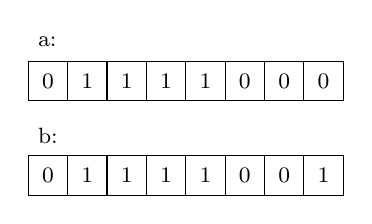
\begin{tikzpicture}
\def\x{0.5}
\def\d{0}
\foreach \i in {0,1,...,7}{
\draw (\i*\x,\d)rectangle(\i*\x+\x,\d+\x);
\ifthenelse{\i=1 \OR \i=2 \OR \i=3 \OR \i=4}
{\node at (\i*\x+0.5*\x,\d+0.5*\x) [] {\footnotesize{1}};}
{\node at (\i*\x+0.5*\x,\d+0.5*\x) [] {\footnotesize{0}};}
}
\node at (0,\d+1.5*\x) [right] {\footnotesize{a:}};

\def\d{-1.2}
\foreach \i in {0,1,...,7}{
\draw (\i*\x,\d)rectangle(\i*\x+\x,\d+\x);
\ifthenelse{\i=1 \OR \i=2 \OR \i=3 \OR \i=4 \OR \i=7}
{\node at (\i*\x+0.5*\x,\d+0.5*\x) [] {\footnotesize{1}};}
{\node at (\i*\x+0.5*\x,\d+0.5*\x) [] {\footnotesize{0}};}
}
\node at (0,\d+1.5*\x) [right] {\footnotesize{b:}};

\end{tikzpicture}
\end{figure}
\end{frame}

\begin{frame}[fragile]\ft{字符变量的存储方式}
由字符变量的存储方式可看出,可以把字符量看成是整型量。事实上,\vspace{0.05in}

\begin{itemize}
\item 
C语言允许对整型变量赋以字符值,也允许对字符型变量赋以整型值。\\[0.1in]
\item 
在输出时,允许把字符变量按整型量输出,也允许把整型量按字符量输出。
\\[0.1in]
\item 
整型量占两个字节,字符量占一个字节,当整型量按字符型量处理时,只有低八位字节参与处理。
\end{itemize}
\end{frame}

\begin{frame}[fragile]\ft{打印字符}
printf()使用格式说明符\lstinline|%c|打印一个字符。若用格式说明符\lstinline|%d|打印字符型变量,将输出一个整数。
\end{frame}

\begin{frame}[fragile]\ft{打印字符}
\lstinputlisting[language=c,numbers=left,frame=single]
{ch03/code/charcode.c}
\end{frame}

\begin{frame}[fragile]\ft{打印字符}
\begin{lstlisting}
$ gcc charcode.c
$ ./a.out
Please input a character:
A
the code for A is 65
\end{lstlisting}
\end{frame}

\begin{frame}[fragile]\ft{打印字符}
\begin{figure}
\centering
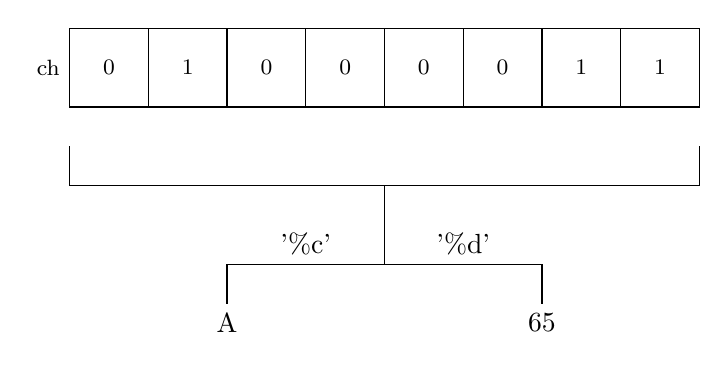
\begin{tikzpicture}
\def\x{1}
\def\d{0}
\foreach \i in {0,1,...,7}{
\draw (\i*\x,\d)rectangle(\i*\x+\x,\d+\x);
\ifthenelse{\i=1 \OR \i=6 \OR \i=7}
{\node at (\i*\x+0.5*\x,\d+0.5*\x) [] {\footnotesize{1}};}
{\node at (\i*\x+0.5*\x,\d+0.5*\x) [] {\footnotesize{0}};}
}
\node at (0,\d+.5*\x) [left] {\footnotesize{ch}};

\draw (0,-0.5*\x)--(0,-\x)--(8*\x,-\x)--(8*\x,-0.5*\x);
\draw (4*\x,-\x)--(4*\x,-2*\x);
\draw (2*\x,-2.5*\x) node[below] {A}
--(2*\x,-2*\x)
--node[above]{'\%c'}(4*\x,-2*\x)
--node[above]{'\%d'}(6*\x,-2*\x)
--(6*\x,-2.5*\x)node[below] {65};

\end{tikzpicture}
\end{figure}

\end{frame}

    \section{浮点型数据}

\begin{frame}\ft{不同计数法}
\begin{table}
\centering
\begin{tabular}{lll} \hline
数字&科学计数法&指数计数法\\\hline
$1~000~000~000$ & $1.0\times 10^9$ & 1.0e9\\ 
$123~000$ & $1.23\times10^5$ & 1.23e5\\
$322.56$ & $3.2256\times10^2$ & 3.2256e2\\
$0.000~056$ & $5.6\times10^{-5}$ & 5.6e-5\\\hline
\end{tabular}
\end{table}
\end{frame}


\begin{frame}\ft{浮点数的存储方式}
C的浮点数包括\lstinline|float|(单精度)、\lstinline|double|(双精度)和\lstinline|long double|类型。 
\end{frame}
%
%
\begin{frame}\ft{浮点数的存储方式}

C标准规定,
\begin{itemize}
\item \lstinline|float|数据占32位,至少能表示6位有效数字,取值范围至少为$10^{-37}$到$10^{+37}$。
\item \lstinline|double|数据占64位,至少能表示10位有效数字,最小取值范围和\lstinline|float|相同。
\item C只保证\lstinline|long double|类型至少同\lstinline|double|类型一样精确。
\end{itemize}
\vspace{0.1in}

两者在存储方式上都遵从IEEE规范,\lstinline|float|遵从IEEE R32.24,而\lstinline|double|遵从IEEE R64.53。
\end{frame}
%
\begin{frame}\ft{浮点数的存储方式}
无论是单精度还是双精度在存储中都分为三个部分:

\begin{enumerate}
\item
符号位(sign):0代表正,1代表负\\[0.1in]
\item 
指数位(exponent):用于存储科学计数法中的指数数据,并采用移位存储\\[0.1in]
\item 
尾数部分(mantissa)
\end{enumerate}
\end{frame}
% %
\begin{frame}\ft{浮点数的存储方式}
\begin{figure}
\centering
\begin{tikzpicture}
\tikzstyle{bracket} = [decoration={brace,amplitude=1em},decorate,thick,black]
\def\x{0.3}

\draw[fill=blue!20] (0,0)rectangle(-32*\x,2*\x);
\draw (-23*\x,0)--(-23*\x,2*\x);
\draw (-31*\x,0)--(-31*\x,2*\x);
\node at (-11*\x,\x) [] {\footnotesize{23}};
\node at (-27*\x,\x) [] {\footnotesize{8}};
\node at (-31.5*\x,\x) [] {\footnotesize{1}};
%%%% 刻度
\draw (-32*\x,-0.2)--(0*\x,-0.2);
\foreach \i in {0,-1,...,-32}
\draw (\i*\x,-0.2)--(\i*\x,-0.1);
\node at (-0.5*\x,-0.2) [below] {\footnotesize{0}};
\node at (-22.5*\x,-0.2) [below] {\footnotesize{22}};
\node at (-30.5*\x,-0.2) [below] {\footnotesize{30}};

\draw[->,red] (-31.5*\x,-1) node[below]{\footnotesize{符号位}}--(-31.5*\x,-0.2);
\draw[->,red] (-26.5*\x,-1) node[below]{\footnotesize{指数位}}--(-26.5*\x,-0.2);
\draw[->,red] (-12.5*\x,-1) node[below]{\footnotesize{尾数部分}}--(-12.5*\x,-0.2);
\draw [bracket] (-32*\x,2*\x)--node[above=1em]{\footnotesize{32位}}(0*\x,2*\x);


\end{tikzpicture}

\caption{\lstinline|float|数据的存储方式}
\end{figure}
\end{frame}
%
\begin{frame}\ft{浮点数的存储方式}
\begin{figure}
\centering
\begin{tikzpicture}[scale=0.95]
\tikzstyle{bracket} = [decoration={brace,amplitude=1em},decorate,thick,black]
\def\x{0.18}

\draw[fill=blue!20] (0,0)rectangle(-64*\x,2*\x);
\draw (-52*\x,0)--(-52*\x,2*\x);
\draw (-63*\x,0)--(-63*\x,2*\x);
\node at (-26*\x,\x) [] {\footnotesize{52}};
\node at (-57.5*\x,\x) [] {\footnotesize{11}};
\node at (-63.5*\x,\x) [] {\footnotesize{1}};
%%%% 刻度
\draw (-64*\x,-0.2)--(0*\x,-0.2);
\foreach \i in {0,-1,...,-64}
\draw (\i*\x,-0.2)--(\i*\x,-0.1);

\node at (-0.5*\x,-0.2) [below] {\footnotesize{0}};
\node at (-51.5*\x,-0.2) [below] {\footnotesize{51}};
\node at (-62.5*\x,-0.2) [below] {\footnotesize{62}};

\draw[->,red] (-63.5*\x,-1) node[below]{\footnotesize{符号位}}--(-63.5*\x,-0.2);
\draw[->,red] (-57.5*\x,-1) node[below]{\footnotesize{指数位}}--(-57.5*\x,-0.2);
\draw[->,red] (-26.5*\x,-1) node[below]{\footnotesize{尾数部分}}--(-26.5*\x,-0.2);
\draw [bracket] (-64*\x,2*\x)--node[above=1em]{\footnotesize{64位}}(0*\x,2*\x);


\end{tikzpicture}

\caption{\lstinline|double|数据的存储方式}
\end{figure}
\end{frame}
%
\begin{frame}\ft{浮点数的存储方式}
R32.24和R64.53的存储方式都用科学计数法来存储数据。

\begin{li}
120.5的二进制表示为1110110.1,二进制科学计数法表示为1.1101101$\times 2^6$。
\end{li}

\end{frame}
%
\begin{frame}\ft{浮点数的存储方式}
\red{任何一个数的二进制科学计数法表示都为
$$
1.****\times 2^n.
$$
因第一位都是1,不存储,故23位的尾数部分,可表示的精度却是24位。 
} 
\end{frame}
%
\begin{frame}\ft{浮点数的存储方式}
 
\begin{wenti}
那么24位能精确到小数点后几位呢? 
\end{wenti}
因$$
(9)_{10}=(1001)_2,
$$
故四位能精确十进制中的1位小数点,24位就能使\lstinline|float|能精确表示到小数点后6位。
\end{frame}
% %
\begin{frame}\ft{浮点数的存储方式}
关于指数部分,因指数可正可负,8位的指数位能表示的指数范围应该是-127~128。所以指数部分的存储采用移位存储,存储的数据为“原数据+127”。
\end{frame}
%
\begin{frame}\ft{浮点数的存储方式}
以下观察8.25的存储方式: 

\begin{enumerate}
\item $8.25$用二进制的科学计数法表示为$1.0001\times2^3$\\[0.1in] \pause 
\item 符号位为:0,表示为正
\item[] 指数位为:$3+127=130=(1000~0010)_2$
\item[] 尾数部分为:$(0001)_2$\\[0.1in]\pause 
\item 存储方式如下:
\begin{figure}
\centering
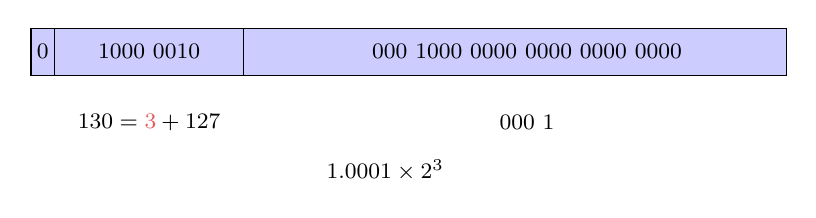
\begin{tikzpicture}
\tikzstyle{bracket} = [decoration={brace,amplitude=1em},decorate,thick,black]
\def\x{0.3}

\draw[fill=blue!20] (0,0)rectangle(-32*\x,2*\x);
\draw (-23*\x,0)--(-23*\x,2*\x);
\draw (-31*\x,0)--(-31*\x,2*\x);
\node at (-11*\x,\x) [] {\footnotesize{000~1000~0000~0000~0000~0000}};
\node at (-27*\x,\x) [] {\footnotesize{1000~0010}};
\node at (-31.5*\x,\x) [] {\footnotesize{0}};

\node at (-27*\x,-2*\x) [] {\footnotesize{$130=\red{3}+127$}};
\node at (-11*\x,-2*\x) [] {\footnotesize{$000~1$}};

\node at (-17*\x,-4*\x) [] {\footnotesize{$1.0001\times 2^3$}};
\end{tikzpicture}
\end{figure}
\end{enumerate}
\end{frame}

\begin{frame}\ft{浮点数的存储方式}
以下观察120.5的存储方式: 

\begin{enumerate}
\item $120.5$用二进制的科学计数法表示为$1.1101101\times2^6$\\[0.1in]\pause 
\item 符号位为:0,表示为正
\item[] 指数位为:$6+127=133=(1000~0101)_2$
\item[] 尾数部分为:$(1101101)_2$\\[0.1in]\pause 
\item 存储方式如下:
\begin{figure}
\centering
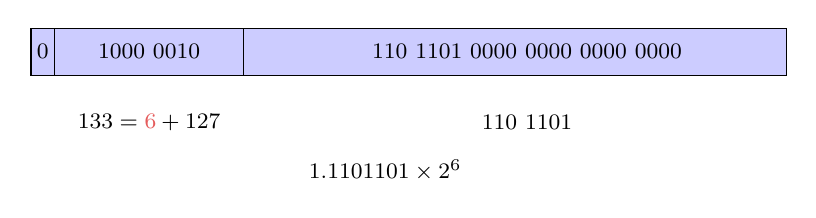
\begin{tikzpicture}
\tikzstyle{bracket} = [decoration={brace,amplitude=1em},decorate,thick,black]
\def\x{0.3}

\draw[fill=blue!20] (0,0)rectangle(-32*\x,2*\x);
\draw (-23*\x,0)--(-23*\x,2*\x);
\draw (-31*\x,0)--(-31*\x,2*\x);
\node at (-11*\x,\x) [] {\footnotesize{110~1101~0000~0000~0000~0000}};
\node at (-27*\x,\x) [] {\footnotesize{1000~0010}};
\node at (-31.5*\x,\x) [] {\footnotesize{0}};

\node at (-27*\x,-2*\x) [] {\footnotesize{$133=\red{6}+127$}};
\node at (-11*\x,-2*\x) [] {\footnotesize{$110~1101$}};

\node at (-17*\x,-4*\x) [] {\footnotesize{$1.1101101\times 2^6$}};
\end{tikzpicture}
\end{figure}
\end{enumerate}
\end{frame}
%
\begin{frame}\ft{浮点数的存储方式}
\begin{wenti}
给出内存中一段数据
$$
0 1000 0101 110 0101 1000 0000 0000 0000,
$$
并告诉你是单精度存储,如何得到该数据的十进制数值?
\end{wenti} 

\end{frame}
%
\begin{frame}\ft{浮点数的存储方式}
\begin{enumerate}
\item 将数据分段
\begin{figure}
\centering
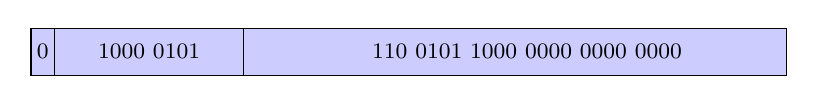
\begin{tikzpicture}
\tikzstyle{bracket} = [decoration={brace,amplitude=1em},decorate,thick,black]
\def\x{0.3}

\draw[fill=blue!20] (0,0)rectangle(-32*\x,2*\x);
\draw (-23*\x,0)--(-23*\x,2*\x);
\draw (-31*\x,0)--(-31*\x,2*\x);
\node at (-11*\x,\x) [] {\footnotesize{110~0101~1000~0000~0000~0000}};
\node at (-27*\x,\x) [] {\footnotesize{1000~0101}};
\node at (-31.5*\x,\x) [] {\footnotesize{0}};
\end{tikzpicture}
\end{figure} \pause 
\item 符号位为0,故为正;因$(1000~0101)_2=133$,故指数为$133-127=6$;故该数据为
$$
(1.1100101\times2^6)_2=(1110010.1)_2=114.5.
$$
\end{enumerate}
\end{frame}
%
\begin{frame}[fragile]\ft{浮点数的存储方式}
阅读如下代码,观察运行结果:
\lstinputlisting[language=c,numbers=left,frame=single]{
ch03/code/float_double.c
}
\end{frame}
%
\begin{frame}[fragile]\ft{浮点数的存储方式}
\begin{lstlisting}
$ gcc float_double.c
$ ./a.out
g1 = 2.2000000476837, g2 = 2.2500000000000
\end{lstlisting}
\end{frame}
%
\begin{frame}[fragile]\ft{浮点数的存储方式}
\begin{wenti}

为什么在单精度转换为双精度时,2.2的数值发生了改变而2.25却没有改变?
\end{wenti} 
\end{frame}
%
\begin{frame}[fragile]\ft{浮点数的存储方式}

\begin{itemize}
\item 2.25的单精度存储方式为
\begin{lstlisting}
0  1000 0001  001 0000 0000 0000 0000
\end{lstlisting}
而双精度存储方式为
\begin{lstlisting}
0  1000 0001  001 0000 0000 0000 0000 0000 0000 0000 0000 0000 0000 0000 0000
\end{lstlisting}
故在强制转换时,数值没有改变。
\end{itemize}

\end{frame}

\begin{frame}[fragile]\ft{浮点数的存储方式}

将十进制小数转换为二进制的方法:\red{将小数乘2,取整数部分。}
\begin{figure}
\centering
\begin{tikzpicture}[scale=0.8]
\matrix[ampersand replacement=\&,matrix of math nodes,column sep=1ex,nodes={inner sep=0.08em}]{
            \& 0 \& .\& 2       \& \&  \\[4pt]
|(a)|\times \&   \&  \&   |(b)|2 \& \&   \\[4pt]
            \& 0 \& .\&  4      \& \& \mbox{取整数位}0 \\[4pt]
|(c)|\times \&   \&  \&  |(d)|2 \& \&   \\[4pt]
            \& 0 \& .\&  8      \& \& \mbox{取整数位}0  \\[4pt]
|(e)|\times \&   \&  \&   |(f)|2 \& \&   \\[4pt]
            \& 1 \& .\&  6      \& \& \mbox{取整数位}1  \\[4pt]                    
|(g)|\times \&   \&  \& |(h)|2 \& \&   \\[4pt]
            \& 1 \& .\& 2      \& \& \mbox{取整数位}1  \\[4pt] 
|(i)|\times \&   \&  \& |(j)|2 \& \&   \\[4pt]
            \& 0 \& .\& 4      \& \& \mbox{取整数位}0  \\[4pt]                                    
};
\draw[thick] (a.south west)--(b.south east)
(c.south west)--(d.south east)
(e.south west)--(f.south east)
(g.south west)--(h.south east)
(i.south west)--(j.south east);
\end{tikzpicture}
\end{figure}
\end{frame}

\begin{frame}[fragile]\ft{浮点数的存储方式}
2.2的二进制表示为一个无限循环的排列:
\begin{lstlisting}
10.0011 0011 0011 0011 0011...
\end{lstlisting}
\end{frame}
%
\begin{frame}[fragile]\ft{浮点数的存储方式}
2.2的单精度存储方式为
\begin{lstlisting}
0  1000 0001  000 1100 1100 1100 1100
\end{lstlisting}
而双精度存储方式为
\begin{lstlisting}
0  1000 0001  000 1100 1100 1100 1100 1100 1100 1100 1100 1100 1100 1100 1100
\end{lstlisting}
故在强制转换时,数值会发生改变。

\end{frame}

\begin{frame}[fragile]\ft{浮点型常量}
基本形式为:
包含小数点的一个带符号的数字序列,接着是字母e或E,然后是代表10的指数的一个有符号值。如
\begin{lstlisting}
-1.56E+12, 2.87e-3
\end{lstlisting}
\end{frame}
%
\begin{frame}[fragile]\ft{浮点型常量}
\begin{itemize}
\item 可以省略正号
\begin{lstlisting}
+2.87e-3
 2.87e-3
\end{lstlisting}
\item 可以没有小数点或指数部分,但不能同时没有
\begin{lstlisting}
2E5
19.28
2     // is an integer
\end{lstlisting}
\item 可以省略小数部分或整数部分,但不能同时省略。
\begin{lstlisting}
3.e12
.45E-5
\end{lstlisting}
\end{itemize}
\end{frame}
%
\begin{frame}[fragile]\ft{浮点型常量}
\begin{itemize}
\item 浮点型常量中不要使用空格
\begin{lstlisting}
1.56 E+12 // wrong
\end{lstlisting}
\item 默认情况下,编译器把浮点型常量当做\lstinline|double|类型。\\[0.1in]
\item[] 设some为一\lstinline|float|变量,
\begin{lstlisting}
some = 4.0 * 2.0;
\end{lstlisting}
则4.0和2.0会被存储为\lstinline|double|类型,用64位存储。
\\[0.1in]
\item[] 注意:乘积运算使用双精度,结果被截取为正常的\lstinline|float|长度,能保证计算精度,但会减慢程序的运行。
\end{itemize}
\end{frame}
%
\begin{frame}[fragile]\ft{浮点型常量}
\begin{itemize}
\item 可以加后缀\lstinline|f|或\lstinline|F|使编译器把浮点常量当做\lstinline|float|型
\begin{lstlisting}
2.3f
3.4e9F
\end{lstlisting}
\item 可以加后缀\lstinline|l|或\lstinline|L|使编译器把浮点常量当做\lstinline|long double|型(由于字母l和数字1容易混淆,建议使用后缀L)
\begin{lstlisting}
54.3l
4.3E9L
\end{lstlisting}
\end{itemize}
\end{frame}

%% add something here
\begin{frame}[fragile]\ft{练习}
\lstinputlisting[language=c,numbers=left,frame=single]{ch03/code/float1.c}
\end{frame}

\begin{frame}[fragile]\ft{练习}
\begin{lstlisting}
$ gcc float1.c
$ ./a.out 
ELSE IF
\end{lstlisting}\pause 


因x为单精度浮点数0.1,常量0.1f表示单精度浮点数0.1,常量0.1f表示双精度浮点数0.1,而根据浮点数的存储方式可知0.1 != 0.1f,故x == 0.1f。
 
\end{frame}



\begin{frame}[fragile]\ft{练习}
\lstinputlisting[language=c,numbers=left,frame=single]{ch03/code/float2.c}
\end{frame}

\begin{frame}[fragile]\ft{练习}
\begin{lstlisting}
$ gcc float2.c
$ ./a.out 
4 8 4
\end{lstlisting}\pause 


原因同上。
\end{frame}


\begin{frame}[fragile]\ft{练习}
\lstinputlisting[language=c,numbers=left,frame=single]{ch03/code/float3.c}
\end{frame}

\begin{frame}[fragile]\ft{练习}
\begin{lstlisting}
$ gcc float2.c
$ ./a.out 
IF
\end{lstlisting}\pause 


因x为单精度浮点数0.5,常量0.1f表示单精度浮点数0.5,常量0.5f表示双精度浮点数0.5,但是根据浮点数的存储方式可知0.5 == 0.5f,故条件x == 0.5先满足,从而执行第一个分支。

\end{frame}

% %
\begin{frame}[fragile]\ft{打印浮点型数据}
\begin{itemize}
\item 使用格式说明符\lstinline|%f|打印\lstinline|float|和\lstinline|double|型数据,{\tf \%e}打印指数计数法的数字。\\[0.1in]
\item 使用格式说明符\lstinline|%Lf|、{\tf \%Le}打印\lstinline|long double|型数据。
\end{itemize}
\end{frame}

\begin{frame}[fragile]\ft{打印浮点型数据}
\lstinputlisting[language=c,numbers=left,frame=single]{ch03/code/showf_pt.c}
\end{frame}

\begin{frame}[fragile]\ft{打印浮点型数据} 
\begin{lstlisting}
$ gcc showf_pt.c
$ ./a.out
32000.000000 can be written as 3.200000e+04
2140000000.000000 can be written as 2.140000e+09
0.000053 can be written as 5.320000e-05
\end{lstlisting}
\end{frame}
%
\begin{frame}[fragile]\ft{浮点型数据的上溢和下溢}
\lstinputlisting[language=c,numbers=left,frame=single]{ch03/code/float_overflow.c}
\end{frame}
%
\begin{frame}[fragile]\ft{浮点型数据的上溢和下溢}\begin{lstlisting}
$ gcc float_overflow.c
$ ./a.out
toobig = inf
\end{lstlisting}

\end{frame}
%
\begin{frame}[fragile]\ft{浮点型数据的上溢和下溢}
当浮点数超出表示范围时,会发生上溢(overflow),C会赋予一个代表无穷大的特殊值,即inf。

\end{frame}
%
\begin{frame}[fragile]\ft{浮点型数据舍入误差}
\lstinputlisting[language=c,numbers=left,frame=single]{ch03/code/float_err.c}
\end{frame}
%
\begin{frame}[fragile]\ft{浮点型数据舍入误差}
\begin{lstlisting}
$ gcc float_err.c
$ ./a.out
b = 4008175468544.000000
\end{lstlisting}
\end{frame}
%
\begin{frame}[fragile]\ft{浮点型数据舍入误差}
为什么会出现如此奇怪的结果?原因是计算机缺乏足够的进行正确运算所需的十进制位数。
\vspace{0.1in}

数字2.0e20加1,变化的是第21位,要计算正确,至少需要存储21位的数字,而\lstinline|float|型数字只有6、7位有效数字,故该计算注定不正确。
\end{frame}
%
% %
% %

  }{}
  \ifthenelse{\equal{#1}{s4}}{
    \section{字符串简介}

\begin{frame}[fragile,allowframebreaks] \ft{示例}
\lstinputlisting[frame=tb,language=C,numbers=left]{
ch04/code/talkback.c
}
\end{frame}


\begin{frame}[fragile] \ft{\secname}
\begin{lstlisting}
Hi! What's your name?
Xiaoping
Xiaoping, what's your weight in pounds?
139
Well, Xiaoping, your volume is 2.23 cubic feet.
Also, your first name has 8 letters, 
and we have 40 bytes to store it in.
\end{lstlisting}
\end{frame}

\begin{frame}[fragile] \ft{\secname}
\begin{dingyi}
字符串(character string)就是一个或多个字符的序列。例如:
\begin{lstlisting}
"Once more you open the door!"
\end{lstlisting}

\end{dingyi}
\vspace{0.1in}

\begin{zhu}
字符串用双引号括起来,但双引号不是字符串的一部分。
\end{zhu}
\end{frame}

\begin{frame} \ft{\secname}
\begin{itemize}
\item
C没有为字符串定义专门的数据类型,而是把它存储在char数组中。
\\[0.2in]
\item
字符串的字符存放在相邻的存储单元中,每个字符占用一个单元。
\\[0.2in]
\item
而数组由相邻存储单元组成,故把字符串存储在数组中是自然的。
\end{itemize}
\end{frame}



\begin{frame}\ft{\secname}
\begin{figure}
\centering
\includegraphics[width=4in]{ch04/images/char_storage.pdf}
\end{figure}
\end{frame}

\begin{frame}[fragile]\ft{\secname}
\begin{itemize}
\item 数组中的最后一个位置显示字符\lstinline|\0|,该字符是空字符(null character),C用它来标记字符串的结束。\\[0.15in]
\item 空字符不是数字0,它是非打印字符,其ASCII码的值为0。\\[0.15in]
\item 空字符的存在意味着数组的单元数至少比要存储的字符数多1。
\end{itemize}

\end{frame}


\begin{frame}\ft{\secname}
\begin{dingyi}
\red{数组(array)}是同一类型的数据元素的有序序列。
\end{dingyi}
\end{frame}


\begin{frame}[fragile]\ft{\secname:如何创建数组?}
\begin{lstlisting}
char name[40];
\end{lstlisting}
该声明语句创建一个有40个存储单元的数组,其中每个单元可存储一个char型值。
\pause \vspace{0.1in}

\begin{itemize}
\item 方括号说明name是一个数组\\[0.1in]
\item 方括号中的40指出数组中的元素个数\\[0.1in]
\item char标识每个元素的类型
\end{itemize}
\end{frame}


\begin{frame}[fragile]\ft{\secname:字符串的使用}
要使用字符串,必须创建一个数组,把字符串中的字符逐个放入数组中,最后还需在结尾添加一个空字符$\backslash$0。
\end{frame}

\begin{frame}[fragile]\ft{\secname:字符串的使用}
\lstinputlisting[language=c,frame=single,numbers=left]{
ch04/code/praise1.c
}
\end{frame}

\begin{frame}[fragile]\ft{\secname:字符串的使用}

\begin{lstlisting}[backgroundcolor=\color{red!10}]
$ gcc praise1.c
$ ./a.out
What's your name?
Xiaoping Zhang
Hello, Xiaoping. What a super marvelous name!
\end{lstlisting}

\end{frame}

\begin{frame}[fragile]\ft{\secname:字符串的使用}
关于\lstinline|scanf()|函数

\begin{itemize}
\item 无须把空字符插入\lstinline|name|数组中,\lstinline|scanf|会在读取输入时完成此任务。\\[0.1in]
\item \lstinline|name|前无须加\lstinline|&|,因为\lstinline|name|本身就是地址。\\[0.1in]
\item 使用\lstinline|%s|的\lstinline|scanf|语句会在遇到的第一个空格、制表符或换行符处停止读取,它只会把第一个单词而不是把整条语句作为字符串读入。\\[0.1in]
\item[] 因此,该程序只读取了Xiaoping。

\end{itemize}
\end{frame}

\begin{frame}[fragile]\ft{\secname:字符与字符串}
请注意\lstinline|"x"|与\lstinline|'x'|的差别\vspace{0.1in}

\begin{itemize}
\item \lstinline|'x'|为字符,而\lstinline|"x"|为字符串\\[0.1in]
\item \lstinline|"x"|由两个字符\lstinline|'x'|和\lstinline|'\0'|组成

\end{itemize}
\end{frame}

\begin{frame}[fragile]\ft{\secname:\lstinline|strlen|函数}
\begin{itemize}
\item 对\lstinline|sizeof|运算符,以字节为单位给出数据大小;\\[0.1in]
\item 对\lstinline|strlen|函数,以字符为单位给出字符串的长度,不包含空字符。

\end{itemize}

\end{frame}

\begin{frame}[fragile,allowframebreaks]\ft{\secname:\lstinline|strlen|函数}
\lstinputlisting[language=c,frame=single,numbers=left]
{
  ch04/code/praise2.c
}
\end{frame}


\begin{frame}[fragile]\ft{\secname:\lstinline|strlen|函数}

\begin{lstlisting}[backgroundcolor=\color{red!10}]
$ gcc praise2.c
$ ./a.out
What's your name?
Xiaoping
Hello, Xiaoping. What a super marvelous name!
Your name of 8 letters occupied 40 memory cells.
The phrase of PRAISE has 28 letters and occpied 29 memory cells.
\end{lstlisting}
\end{frame}

\begin{frame}[fragile]\ft{\secname:\lstinline|strlen|函数}
\begin{itemize}
\item 头文件\lstinline|string.h|包含许多与字符串相关的函数的原型,包括\lstinline|strlen|函数。\\[0.1in]
\item C把函数库分成多个相关函数的序列,并为每个序列提供一个头文件。比如:\\[0.1in]
\item[(1)] \lstinline|printf|和\lstinline|scanf|属于标准输入输出序列,使用\lstinline|stdio.h|。\\[0.1in]
\item[(2)] \lstinline|strlen|和其它一些与字符串相关的函数同属一个系列,使用\lstinline|string.h|。
\end{itemize}
\end{frame}

\begin{frame}[fragile]\ft{\secname:printf函数处理长字符串}
\begin{itemize}
\item 一条\lstinline|printf|语句占用两行,但只能在参数之间断行,不允许在字符串中间断行。\\[0.1in]
\item 使用两个\lstinline|printf|语句输出一行,换行符只出现在第二条语句。
\end{itemize}
\end{frame}

\begin{frame}[fragile]\ft{\secname:\lstinline|sizeof|运算符与\lstinline|strlen|返回值}
设\lstinline|name = "Morgan"|,则
\begin{lstlisting}[backgroundcolor=\color{red!10}]
sizeof name : 40
strlen(name): 6
\end{lstlisting}

\begin{figure}
\centering
\includegraphics[]{ch04/images/morgan}
\end{figure}
\end{frame}

\begin{frame}[fragile]\ft{\secname:sizeof运算符与strlen返回值}
\begin{lstlisting}[backgroundcolor=\color{red!10}]
sizeof PRAISE : 29
strlen(PRAISE): 28
\end{lstlisting}

\lstinline|sizeof|运算符在处理字符串变量时,会将空字符也计算在内。
\end{frame}

\begin{frame}[fragile]\ft{\secname:\lstinline|sizeof|运算符后的圆括号}
\begin{itemize}
\item 圆括号对于数据类型是必需的,而对于具体量则是可选的。
\begin{lstlisting}[backgroundcolor=\color{red!10}]
sizeof(float)
sizeof(char)

sizeof name
sizeof 2.15
\end{lstlisting}
\item 建议在所有情况下都使用圆括号。
\begin{lstlisting}[backgroundcolor=\color{red!10}]
sizeof(name)
sizeof(2.15)
\end{lstlisting}
\end{itemize}
\end{frame}


    \section{常量与预处理器}

\begin{frame}[fragile]\ft{\secname}
\lstinputlisting[language=c,frame=single,numbers=left]
{ch04/code/circle1.c}
\end{frame}

\begin{frame}[fragile]\ft{\secname}
\begin{lstlisting}[backgroundcolor=\color{red!10}]
radius =  1.000000, circum = 6.283185, area = 3.141593
\end{lstlisting}
\end{frame}

\begin{frame}[fragile]\ft{\secname}
\lstinputlisting[language=c,frame=single,numbers=left]
{ch04/code/circle2.c}
\end{frame}

\begin{frame}[fragile]\ft{\secname}
\lstinputlisting[language=c,frame=single,numbers=left]
{ch04/code/circle3.c}
\end{frame}

\begin{frame}[fragile]\ft{\secname}
\lstinputlisting[language=c,frame=single,numbers=left]
{ch04/code/circle4.c}

\end{frame}

\begin{frame}[fragile]\ft{\secname:宏定义}
\begin{lstlisting}[title=宏定义的一般形式,backgroundcolor=\color{red!10}]
#define NAME value
\end{lstlisting}

\begin{itemize}
\item 没有使用分号是因为这是一种替代机制,而不是C的语句。\\[0.1in]
\item 符号常量请使用大写,其好处在于当看到它时便可立即知道是常量。\\[0.1in]
\item 符号常量的命名请遵循变量命名规则。
\end{itemize}
\end{frame}

\begin{frame}[fragile]\ft{\secname:宏定义}
\lstinline|#define|语句也可用于定义字符和字符串变量,前者用单引号,后者用双引号。
\vspace{0.1in}

\begin{lstlisting}
#define BEEP '\a'
#define TEE 'T'
#define ESC '\033'
#define OOPS "Now you have done it!"
\end{lstlisting}

\end{frame}

\begin{frame}[fragile]\ft{\secname:宏定义}
\lstinline|#define|语句也可用于定义字符和字符串变量,前者用单引号,后者用双引号。
\vspace{0.1in} \pause 

\begin{lstlisting}[title=常见错误]
#define B = 20
\end{lstlisting}
\vspace{0.1in}

如果这样做,\lstinline|B|将会被\lstinline|= 20|而不是\lstinline|20|代替。 这样以下语句
\begin{lstlisting}
c = a + B;
\end{lstlisting}
会被替换成如下错误的表达:
\begin{lstlisting}
c = a + = 20;
\end{lstlisting}
\end{frame}

\begin{frame}[fragile]\ft{\secname:\lstinline|const|修饰符}
C90允许使用关键字\lstinline|const|把一个变量声明转换为常量声明:
\begin{lstlisting}
const int MONTHS = 12; 
\end{lstlisting}
这使得\lstinline|MONTHS|成为一个只读值。你可以显示它,并把它用于计算中,但不能改变它的值。
\end{frame}

    \section{格式化输出}

\begin{frame}[fragile]\ft{\secname}
\begin{table}
\centering
\caption{格式说明符}
\begin{tabular}{p{2.5cm}|p{7.5cm}} \hline
格式说明符 & ~~~~~~~~输出 \\ \hline\hline 
 \lstinline|%a| & 浮点数、十六进制和p-计数法 \\
 \lstinline|%A| & 浮点数、十六进制和P-计数法 \\
 \lstinline|%c| & 一个字符\\
 \lstinline|%d| & 有符号十进制数\\\hline
\end{tabular}
\end{table}
\end{frame}


\begin{frame}[fragile]\ft{\secname}
\begin{table}
\centering
\caption{格式说明符}
\begin{tabular}{p{2.5cm}|p{7.5cm}} \hline
格式说明符 & ~~~~~~~~输出 \\ \hline\hline 
 \lstinline|%e| & 浮点数、e-计数法\\
 \lstinline|%E| & 浮点数、E-计数法\\
 \lstinline|%f| & 浮点数、十进制计数法\\
 \lstinline|%g| & 根据数值不同自动选\lstinline|%f|或\lstinline|%e|。\lstinline|%e|格式在指数小于-4或大于等于精度时使用\\
 \lstinline|%G| & 根据数值不同自动选\lstinline|%f|或\lstinline|%E|。\lstinline|%E|格式在指数小于-4或大于等于精度时使用\\\hline
\end{tabular}
\end{table}
\end{frame}

\begin{frame}[fragile]\ft{\secname}
\begin{table}
\centering
\caption{格式说明符}
\begin{tabular}{p{2.5cm}|p{7.5cm}} \hline
格式说明符 & ~~~~~~~~输出 \\ \hline\hline 
\lstinline|%i| & 有符号十进制整数(同\lstinline|%d|)\\
\lstinline|%o| & 无符号八进制整数\\
\lstinline|%p| & 指针\\
\lstinline|%s| & 字符串\\\hline
\end{tabular}
\end{table}
\end{frame}


\begin{frame}[fragile]\ft{\secname}
\begin{table}
\centering
\caption{格式说明符}
\begin{tabular}{p{2.5cm}|p{7.5cm}} \hline
格式说明符 & ~~~~~~~~输出 \\ \hline\hline 
\lstinline|%x| & 使用十六进制数字0-f的无符号十六进制整数\\
\lstinline|%X| & 使用十六进制数字0-F的无符号十六进制整数\\
\hline
\end{tabular}
\end{table}
\end{frame}

\begin{frame}[fragile]\ft{\secname}
\begin{lstlisting}[title=printf的使用格式]
printf(Control-string, item1, item2, ...);
\end{lstlisting} \vspace{0.1in}

\begin{itemize}
\item item1, item2等是要打印的项目,它们可以是变量,也可以是常量,甚至是在打印之前进行计算的表达式。\\[0.1in]
\item 控制字符串(Control-string)是一个描述项目如何打印的字符串,它为每个要打印的项目包含一个格式说明符。

\end{itemize}
\end{frame}

\begin{frame}[fragile]\ft{\secname}
\begin{figure}
\centering
\includegraphics[]{ch04/images/printf.pdf}
\end{figure}

\vspace{.1in} \pause 

\red{不要忘记给控制字符串后面的列表中的每个项目都使用一个格式说明符。}
\end{frame}

\begin{frame}[fragile]\ft{\secname}
\begin{itemize}
\item 如果只打印一个语句,则不需要任何格式说明符;\\[0.1in]
\item 如果只打印数据,则无须加入任何说明内容。\\[0.1in]
\item 想打印\lstinline|%|,必须使用两个\lstinline|%%|符号。
\end{itemize}

\begin{lstlisting}
printf("Once more you open the door!\n");
printf("%s%d\n", "area = ", area);
printf("%d%% = %f\n", 30, 0.3);
\end{lstlisting}
\end{frame}

\begin{frame}[fragile]\ft{\secname: \lstinline|\%d|}
\begin{itemize}
\item \lstinline|%d|:  按整型数据的实际长度输出\\[0.1in]
\item \lstinline|%md|:  输出字段的宽度为m,右对齐\\ 
\item[] 若数据位数<m,左端补空格;若>=m,按实际位数输出。\\[0.1in]
\item \lstinline|%-md|: 输出字段的宽度为m,左对齐\\ 
\item[] 若数据位数<m,右端补空格;若>=m,按实际位数输出。\\[0.1in]
\item \lstinline|%0md|: 输出字段的宽度为m,右对齐 \\ 
\item[] 若数据位数<m,右端补0;若>=m,按实际位数输出。
\end{itemize}
\end{frame}

\begin{frame}[fragile]\ft{\secname: \lstinline|\%d|}
\lstinputlisting[language=c,frame=single,numbers=left]{ch04/code/width.c}
\end{frame}

\begin{frame}[fragile]\ft{\secname: \lstinline|\%d|}
\begin{lstlisting}[showspaces=true,backgroundcolor=\color{red!20}]
*1000*
*1000*
*      1000*
*1000      *
*0000001000*
\end{lstlisting}
\end{frame}


\begin{frame}[fragile,allowframebreaks]\ft{\secname: \lstinline|\%f|、\lstinline|\%e|和\lstinline|\%E|}
\lstinputlisting[language=c,numbers=left]
{ch04/code/floats.c}
\end{frame}

\begin{frame}[fragile]\ft{\secname: \lstinline|\%f|、\lstinline|\%e|和\lstinline|\%E|}
\begin{lstlisting}[showspaces=true,backgroundcolor=\color{red!20}]
*3852.990000*
*3.852990e+03*
*3852.99*
*3853.0*
*  3852.990*
* 3.853e+03*
* 3.853E+03*
*+3852.99*
*3852.99   *
*0003852.99*
\end{lstlisting}
\end{frame}

\begin{frame}[fragile]\ft{\secname: \lstinline|\%f|、\lstinline|\%e|和\lstinline|\%E|}
\begin{lstlisting}[backgroundcolor=\color{red!20}]
%m.nf     %m.ne      %m.nE
\end{lstlisting}

\begin{itemize}
\item m:字段宽度
\item n:小数点后面数字的个数
\end{itemize}
\end{frame}

\begin{frame}[fragile]\ft{\secname: \lstinline|\%f|、\lstinline|\%e|和\lstinline|\%E|}
\begin{lstlisting}[backgroundcolor=\color{red!20}] 
%.nf
\end{lstlisting}

\begin{itemize}
\item  整数部分以实际长度输出
\item n:小数点后面数字的个数
\end{itemize}
\end{frame}

\begin{frame}[fragile]\ft{\secname: \lstinline|\%f|、\lstinline|\%e|和\lstinline|\%E|}
\begin{lstlisting}[backgroundcolor=\color{red!20}] 
%m.f
\end{lstlisting}

\begin{itemize}
\item m: 字段宽度
\item 不输出小数点后的数字
\end{itemize}
\end{frame}

\begin{frame}[fragile]\ft{\secname: \lstinline|\%d|}
    \lstinputlisting[language=c,numbers=left]{ch04/code/flags.c}    
\end{frame}

\begin{frame}[fragile]\ft{\secname: \lstinline|\%d|}
\begin{lstlisting}[showspaces=true,backgroundcolor=\color{red!20}]
1f 1F 0x1f 0X1F
*42*
* 42*
*-42*
*    6*
*  006*
*00006*
*  006*
\end{lstlisting}
\end{frame}


\begin{frame}[fragile] \ft{\secname: \lstinline|\%d|}
 使用\lstinline|% d|在正值之前产生一个前导空格,在负值之前不产生前导空格。
这使得有效位相同的正值和负值以相同字段宽度打印输出。
\end{frame}

\begin{frame}[fragile]\ft{\secname: \lstinline|\%d|} 
\begin{itemize}
\item \lstinline|%5.3d|为精度说明符,用于在整数格式中来产生足够的前导零以填满要求的最小数字位数。\\[0.1in]
\item \lstinline|%05d|将会用前导零填满整个字段宽度。\\[0.1in]
\item 在\lstinline|%05.3d|中,0标志和精度说明符同时出现,此时0标志将会忽略。
\end{itemize}
\end{frame}

\begin{frame}[fragile]\ft{\secname: \lstinline|\%s|}
\lstinputlisting[language=c,,numbers=left]{ch04/code/strings.c}    
\end{frame}

\begin{frame}[fragile]\ft{\secname: \lstinline|\%s|}
\begin{lstlisting}[showspaces=true,backgroundcolor=\color{red!20}]
*Hello World!*
*   Hello World!*
*          Hello*
*Hello          *
\end{lstlisting}
\end{frame}

\begin{frame}[fragile]\ft{\secname: \lstinline|\%s|}
\lstinline|%15.5s|为精度说明符,告诉printf函数只打印5个字符。修饰符‘-’使文本左对齐输出。
\end{frame}

\begin{frame}[fragile]\ft{\secname:\lstinline|printf()|的返回值}
\lstinputlisting[language=c,,numbers=left]{ch04/code/printval.c}
\end{frame}

\begin{frame}[fragile]\ft{\secname:\lstinline|printf()|的返回值}
\begin{lstlisting}[backgroundcolor=\color{red!20}]
100 C is water's boiling point.
the printf function printed 32 character.
\end{lstlisting}
\end{frame}

\begin{frame}[fragile]\ft{\secname:\lstinline|printf()|的返回值}
\lstinline|printf()|返回所有打印字符的个数,包括空格和不可见的换行字符。
\end{frame}


\begin{frame}[fragile]\ft{\secname:\lstinline|printf()|中的\lstinline|\%n|}
  在\lstinline|printf()|中,\lstinline|%n|是一个格式化说明符,它将获取\lstinline|%n|出现之前的所有字符的个数,并将其传递给后面对应的变量。
\end{frame}


\begin{frame}[fragile]\ft{\secname:\lstinline|printf()|中的\lstinline|\%n|}
\lstinputlisting[language=c,,numbers=left]{ch04/code/printf_n.c}
\end{frame}


\begin{frame}[fragile]\ft{\secname:\lstinline|printf()|中的\lstinline|\%n|}
\begin{lstlisting}[backgroundcolor=\color{red!20}]
$ gcc printf_n.c
$ ./a.out 
Hello Wuhan University!
c1 = 12, c2 = 23
\end{lstlisting}
\end{frame}




    \section{格式化输入}
\begin{frame}[fragile]\ft{\secname}
  同\lstinline|printf()|一样,\lstinline|scanf()|也使用控制字符串和参数列表,主要区别在参数列表。\lstinline|printf()|使用变量名、常量和表达式;而\lstinline|scanf()|使用指向变量的指针。
\end{frame}

\begin{frame}[fragile]\ft{\secname:\lstinline|scanf()|的参数列表}
\begin{itemize}
\item 
  若使用\lstinline|scanf()|来读取某种基本类型的值,请在变量名前加一个\lstinline|&|。 \\[0.1in]
\item
  若使用\lstinline|scanf()|把一个字符串读入一个字符数组,请不要使用\lstinline|&|。
\end{itemize}
\end{frame}

\begin{frame}[fragile]\ft{\secname:\lstinline|scanf()|的参数列表}
\lstinputlisting[language=c,frame=single,numbers=left]{ch04/code/input.c}
\end{frame}

\begin{frame}[fragile]\ft{\secname:\lstinline|scanf()|的参数列表}
\begin{lstlisting}[backgroundcolor=\color{red!20}]
$ gcc input.c
$ ./a.out
Enter your name, age and weight:
Xiaoming 23, 100
Xiaoming: 23 100.000000
\end{lstlisting}
\end{frame}

\begin{frame}[fragile]\ft{\secname:\lstinline|scanf()|的参数列表}
\begin{itemize}
\item
 \lstinline|scanf()|使用空格(换行、制表符和空格)来决定如何把输入分成几个字段。
它依次把格式说明符与字段相匹配,并跳过它们之间的空格。\\[0.1in]
\item
也可以分一行或多行输入,只要每个输入项目之间至少有一个换行符、空格或制表符。\\[0.1in]
\item
\%c是个例外,即使下一个字符是空白字符,它也会读取。
\end{itemize}
\end{frame}

\begin{frame}[fragile]\ft{\secname:\lstinline|printf|与\lstinline|scanf|格式说明符的区别}
\begin{itemize}
\item
  \lstinline|printf()|把\lstinline|%f|、\lstinline|%e|、\lstinline|%E|、\lstinline|%g|和\lstinline|%G|同时用于\lstinline|float|和\lstinline|double|类型\\[0.1in]
\item
\lstinline|scanf()|只把它们用于\lstinline|float|类型,而用于\lstinline|double|类型时要求加上l修饰符。
\end{itemize}
\end{frame}

\begin{frame}[fragile]\ft{\secname:\lstinline|scanf|格式说明符}
\begin{table}
\centering
\begin{tabular}{p{3cm}|p{7cm}}\hline
格式说明符 & 意义 \\\hline\hline
\lstinline|%c| & 把输入解释成一个字符 \\[2mm]
\lstinline|%d| & 把输入解释成一个有符号十进制数 \\[2mm]
\lstinline|%e|,\lstinline|%f|,\lstinline|%g|,\lstinline|%a| & 把输入解释成一个浮点数\\[2mm]
\lstinline|%E|,\lstinline|%f|,\lstinline|%g|,\lstinline|%A| & 把输入解释成一个浮点数\\[2mm]
\lstinline|%i| & 把输入解释成一个有符号十进制数\\[2mm]
\lstinline|%o| & 把输入解释成一个有符号八进制数\\[2mm]
\lstinline|%p| & 把输入解释成一个指针\\ \hline
\end{tabular}
\end{table}
\end{frame}

\begin{frame}[fragile]\ft{\secname:\lstinline|scanf|格式说明符}
\begin{table}
\centering
\begin{tabular}{p{2cm}|p{8cm}}\hline
格式说明符 & 意义 \\\hline\hline
\lstinline|%s| & 把输入解释成一个字符串:输入内容以第一个非空白字符作为开始,并且包含到下一个空白字符的全部字符 \\[2mm]
\lstinline|%u| & 把输入解释成一个无符号十进制数 \\[2mm]
\lstinline|%x|,\lstinline|%X| & 把输入解释成一个有符号十六进制数\\ \hline
\end{tabular}
\end{table}
\end{frame}

\begin{frame}[fragile]\ft{\secname:\lstinline|scanf|格式说明符}
 可在格式说明符中使用修饰符,修饰符出现在\%与格式字符之间。
\end{frame}

\begin{frame}[fragile]\ft{\secname:\lstinline|scanf|格式说明符}

\begin{table}
\centering
\begin{tabular}{p{2cm}|p{8cm}}\hline
修饰符 & 意义 \\\hline\hline
 * &  滞后赋值,如{" \%*d"} \\[2mm]
 digit & 最大字段宽度:在达到最大字段宽度或遇到第一个空白字符时停止对输入项的读取,如{ "\%10s"} \\[2mm]
 hh & 把整数读作{ signed char}或{ unsigned char},如{ "\%hhd"}或{ "\%hhu"} \\[2mm]
 ll & 把整数读作{ long long}或{ unsigned long long},如{ "\%lld"}或{ "\%llu"}\\
\hline
\end{tabular}
\end{table}
\end{frame}

\begin{frame}[fragile]\ft{\secname:\lstinline|scanf|格式说明符}
\begin{table}
\centering
%\caption{修饰符h, l 或 L}
\begin{tabular}{p{3.5cm}|p{6cm}}\hline
修饰符 & 意义 \\\hline\hline
 "\lstinline|%hd|", "\lstinline|%hi|" & 以\lstinline|short|存储 \\[2mm]\hline
 "\lstinline|%ho|", "\lstinline|%hx|", "\lstinline|%hu|" & 以\lstinline|unsigned short|存储\\[2mm]\hline
 "\lstinline|%ld|", "\lstinline|%li|" & 以\lstinline|long|存储\\[2mm]\hline
 "\lstinline|%lo|", "\lstinline|%lx|", "\lstinline|%lu|" & 以\lstinline|unsigned long|存储\\[2mm]\hline
 "\lstinline|%le|", "\lstinline|%lf|", "\lstinline|%lg|" & 以\lstinline|double|存储
\\[2mm]\hline
 "\lstinline|%Le|", "\lstinline|%Lf|", "\lstinline|%Lg|" & 以\lstinline|long double|存储 \\
\hline
\end{tabular}
\end{table}
\end{frame}

\begin{frame}[fragile]\ft{\secname:\lstinline|scanf|格式说明符}
  若没有这些修饰符,则\lstinline|%d|, \lstinline|%i|, \lstinline|%o|和\lstinline|%x|指示\lstinline|int|类型,而\lstinline|%e|, \lstinline|%f|和\lstinline|%g|指示\lstinline|float|类型。
\end{frame}

\begin{frame}[fragile]\ft{\secname:格式字符串中的常规字符}
  \lstinline|scanf()|允许把普通字符放在格式字符串中,除了空格字符之外的普通字符一定要与输入字符串准确匹配。  
\end{frame}

\begin{frame}[fragile]\ft{\secname:格式字符串中的常规字符}
\begin{lstlisting}[showspaces=true,backgroundcolor=\color{red!20}]
scanf("%d, %d", &n, &m);
\end{lstlisting}

\rule{\textwidth}{0.1em}
\begin{lstlisting}[title=合法的输入方式,showspaces=true,backgroundcolor=\color{red!20}]
12, 23

12,     23

12 , 23

12,
23
\end{lstlisting}

\end{frame}

\begin{frame}[fragile]\ft{\secname:格式字符串中的常规字符}
\begin{lstlisting}[showspaces=true,backgroundcolor=\color{red!20}]
scanf("%d and %d", &n, &m);
\end{lstlisting}

\rule{\textwidth}{0.1em}
\begin{lstlisting}[title=合法的输入方式,showspaces=true,backgroundcolor=\color{red!20}]
12 and 23

12 and     23

12and23
\end{lstlisting}
\end{frame}

\begin{frame}[fragile]\ft{\secname:格式字符串中的常规字符}

除了\lstinline|%c|之外的说明符会自动跳过输入项之前的空格,故以下两条语句的效果相同:
\begin{lstlisting}[showspaces=true,backgroundcolor=\color{red!10}]
scanf("%d%d",&n,&m);

scanf("%d %d",&n,&m);
\end{lstlisting}
\end{frame}

\begin{frame}[fragile]\ft{\secname:格式字符串中的常规字符}
对于\lstinline|%c|来说,向格式字符串中添加一些空格将导致一些差别。如:
\begin{lstlisting}[showstringspaces=true,backgroundcolor=\color{red!10}]
scanf("%c", &ch);
\end{lstlisting}
读取在输入中遇到的第一个字符,而
\begin{lstlisting}[showstringspaces=true,backgroundcolor=\color{red!10}]
scanf(" %c", &ch);
\end{lstlisting}
则读取遇到的第一个非空白字符。
\end{frame}

\begin{frame}[fragile]\ft{\secname:\lstinline|scanf|的返回值}
\lstinline|scanf()|返回成功读入的项目个数。

\begin{itemize}
\item
 若没有读取任何项目,则返回0;
\item
若检测到文件结尾(end of file),则返回\lstinline|EOF|。
(\lstinline|EOF|是stdio.h中定义的特殊值,一般为-1)
\end{itemize}

\end{frame}

\begin{frame}[fragile,allowframebreaks]\ft{\secname:\lstinline|printf()|的*修饰符}
\lstinputlisting[language=c,frame=single,numbers=left]{ch04/code/varwidth.c}
\end{frame}

\begin{frame}[fragile]\ft{\secname:printf的*修饰符}
\begin{lstlisting}[backgroundcolor=\color{red!10}]
$ gcc varwidth.c
$ ./a.out
What field width?
6
The number is:   256
Now enter a width and a precision:
8 3
Weight= 123.500
\end{lstlisting}
\end{frame}

\begin{frame}[fragile]\ft{\secname:\lstinline|scanf()|的*修饰符}
在\lstinline|scanf()|中,把\lstinline|*|放在\lstinline|%|与格式字符之间时,会使函数跳过相应的输入项目。
\end{frame}

\begin{frame}[fragile]\ft{\secname:\lstinline|scanf()|的*修饰符}

\lstinputlisting[language=c,frame=single,numbers=left]{ch04/code/skip2.c}
\end{frame}

\begin{frame}[fragile]\ft{\secname:\lstinline|scanf()|的*修饰符}
\begin{lstlisting}[backgroundcolor=\color{red!10}]
$ gcc skip2.c
$ ./a.out
Please enter three integers:
10 20 30
The last integer was 30
\end{lstlisting}
\end{frame}






  }{}
  \ifthenelse{\equal{#1}{s5}}{
    \section{示例程序}

\begin{frame}[fragile]\ft{\secname}
\lstinputlisting[language=c,numbers=left]{ch05/code/shoe1.c} 

\end{frame}


\begin{frame}[fragile]\ft{\secname}
\begin{lstlisting}[backgroundcolor=\color{red!10}]
$ gcc shoe1.c
$ ./a.out 
Shoe size (men's)   foot length
       9.0           10.56 inches
\end{lstlisting}
\end{frame}


\begin{frame}[fragile,allowframebreaks]\ft{\secname}
\lstinputlisting[language=c,frame=single,numbers=left]{ch05/code/shoe2.c} 
\end{frame}



\begin{frame}[fragile]\ft{\secname}
\begin{lstlisting}[backgroundcolor=\color{red!10}]
$ gcc shoe2.c
$ ./a.out 
Shoe size (men's)  foot length
      12.0           11.54 inches
      13.0           11.87 inches
      14.0           12.19 inches
      15.0           12.52 inches
      16.0           12.84 inches
      17.0           13.16 inches
      18.0           13.49 inches
If shoes fit, wear it.
\end{lstlisting}
\end{frame}


\begin{frame}[fragile]\ft{while循环}
\begin{lstlisting}[language=c,frame=single]
while (condition)
  statement
\end{lstlisting}

\begin{lstlisting}[language=c,frame=single]
while (condition)
{
  statements
}
\end{lstlisting}

\begin{lstlisting}[language=c,frame=single]
while (condition){
  statements
}
\end{lstlisting}


\end{frame}


\begin{frame}[fragile]\ft{while循环}
\begin{figure}
\centering
\includegraphics[width=3in]{ch05/images/while.pdf}
\end{figure}
\end{frame}

    %%%%%%%%%
\section{基本运算符}

\subsection{赋值运算符}
\begin{frame}[fragile]\ft{\subsecname}
\begin{lstlisting}[language=c,backgroundcolor=\color{red!10}]
  int n; 
  n = 2016;
\end{lstlisting} \pause 

\begin{itemize}
\item 在C中,\lstinline|=| 是一个赋值运算符(assignment operator),不表示“相等”。\\[0.15in]
\item 请读成“将值2016赋给变量n”,而不是“n等于2016”。\\[0.15in]
\item 赋值运算符的动作是从右到左。
\end{itemize}

\end{frame}

\begin{frame}[fragile]\ft{\subsecname}
\begin{lstlisting}[language=c,backgroundcolor=\color{red!10}]
  i = i + 1;
\end{lstlisting} \pause 
\begin{figure}
\centering
\includegraphics[width=3in]{ch05/images/assign.pdf}
\end{figure}
\end{frame}

\begin{frame}[fragile]\ft{\subsecname}
以下语句没有意义:
\begin{lstlisting}[language=c,backgroundcolor=\color{red!10}]
  2016 = n;
\end{lstlisting} 	
因不能将一个值赋给常量。
\end{frame}

\begin{frame}[fragile]\ft{\subsecname}
\begin{enumerate}
\item 左值: 指向内存位置的表达式称为\red{左值表达式}。\\[0.4cm]
\item[] 左值可以是变量名或表达式,但表达式必须表示的是个内存位置。\\[0.4cm]
\item 右值: 存储在内存中某些位置的数值。\\[0.4cm]
\item 操作数:运算符操作的对象。
\end{enumerate}
\end{frame}


\begin{frame}[fragile]\ft{\subsecname}
\lstinputlisting[language=c,frame=single,numbers=left]{ch05/code/AssignOpThree.c}
\end{frame}


\begin{frame}[fragile]\ft{\subsecname}
\begin{lstlisting}[backgroundcolor=\color{red!10}]    
$ gcc AssignOpThree.c
$ ./a.out
a = 10, b = 10, c = 10  
\end{lstlisting}

\pause \vspace{.1in}

赋值的过程是从右到左的。先将10赋给c,再将c的值赋给b,最后将b的值赋给a。
\end{frame}

\subsection{加减运算符}
\begin{frame}[fragile]\ft{\subsecname}
加法运算符(addition operator)将其两侧的操作数进行相加。 \vspace{1em}

\begin{lstlisting}
printf("%d", 4+20);
\end{lstlisting}
\vspace{1em}

两个操作数可以是变量,也可以是常量,如
\begin{lstlisting}
c = a + b;
\end{lstlisting}
\end{frame}
 
\begin{frame}[fragile]\ft{\subsecname}
减法运算符(subtraction operator)将它前面的数减去后面的数。\vspace{1em}

\begin{lstlisting}
b = 20.0 - 200.0;
\end{lstlisting}
\vspace{1em}

\lstinline|+| 和 \lstinline|-| 运算符被称为双目运算符,因为它们都需要两个操作数。
\end{frame}


\begin{frame}[fragile]\ft{\subsecname}
\lstinline|+| 和 \lstinline|-| 也可以用作单目运算符。
\vspace{1em}

\begin{lstlisting}[language=c,backgroundcolor=\color{red!10}]
a = -1;
b = -a;
\end{lstlisting}
此时 \lstinline|-| 表示负号,用于指示或改变一个值的符号。
\vspace{1em}

C99引入了单目运算符 \lstinline|+|,它不改变操作数的值或符号:
\begin{lstlisting}[language=c,backgroundcolor=\color{red!10}]
a = +1;
\end{lstlisting}
\end{frame}

\subsection{乘法运算符}
\begin{frame}[fragile]\ft{\subsecname}
\begin{lstlisting}[language=c,backgroundcolor=\color{red!10}]
  mile = 1.6 * km;
\end{lstlisting}
\vspace{1em}

\red{注意:C没有提供计算平方的运算符。}
\end{frame}


\begin{frame}[fragile]\ft{\subsecname}

\lstinputlisting[language=c,numbers=left]{ch05/code/squares.c}
\end{frame}


\begin{frame}[fragile]\ft{\subsecname}
\begin{lstlisting}[backgroundcolor=\color{red!10}]
$ gcc squares.c
$ ./a.out 
   1^2 =      1
   2^2 =      4
   3^2 =      9
   4^2 =     16
   5^2 =     25
   6^2 =     36
   7^2 =     49
   8^2 =     64
   9^2 =     81
\end{lstlisting}
\end{frame}



\subsection{除法运算符}
\begin{frame}[fragile]\ft{\subsecname}
  \lstinputlisting[language=c,numbers=left]{ch05/code/divide.c}    
\end{frame}
\begin{frame}[fragile]\ft{\subsecname}
\begin{lstlisting}[backgroundcolor=\color{red!10}]
$ gcc divide.c
$ ./a.out  
3 / 4 = 0
6 / 3 = 2
7 / 4 = 1
7. / 4. = 1.75
7. / 4  = 1.75
\end{lstlisting}    
\end{frame}




\begin{frame}[fragile]\ft{\subsecname}
\begin{itemize}
\item 整数相除,其结果的小数部分会被丢弃,称之为截尾。\\[0.1in]
\item 浮点数相除会得到一个浮点数结果。\\[0.1in]
\item C允许用一个整数去除浮点数,其结果也是浮点数。在此情况下,做除法运算之前会将整数化为浮点数。
\end{itemize}
\end{frame}

\subsection{运算符优先级}
\begin{frame}[fragile]\ft{\subsecname}
\begin{table}
\centering
\begin{tabular}{c|c} \hline
运算符& 结合性\\\hline\hline
\lstinline|()| & 从左到右 \\\hline
\lstinline|+, -|(单目运算符) & 从右到左\\\hline
\lstinline|*, /| & 从左到右 \\\hline
\lstinline|+, -|(双目运算符) & 从左到右 \\\hline
\lstinline|=| & 从右到左\\\hline
\end{tabular}
\end{table}
\end{frame}


\begin{frame}[fragile]\ft{\subsecname}
\begin{lstlisting}[frame=no,backgroundcolor=\color{red!10}]
y = 6 * 12 + 5 * 20;
\end{lstlisting}

\rule{\textwidth}{1mm}\pause 

\begin{itemize}
\item 根据优先级规定,两个乘法运算在加法运算之前进行。\\[0.1in]
\item 至于两个乘法运算谁先进行,C将此选择权留给实现者。
\end{itemize}

\end{frame}

\begin{frame}[fragile]\ft{\subsecname}
\begin{lstlisting}[frame=no,backgroundcolor=\color{red!10}]
y = 12 / 3 * 2;
\end{lstlisting}
\rule{\textwidth}{1mm}\pause 

\begin{itemize}
\item 结合规则适用于\red{共享同一操作数的运算符}。\\[0.1in]
\item  \lstinline|/| 和 \lstinline|*| 优先级相同,它们共享操作数3,按“从左到右”的结合原则,应该先算12/3。
\end{itemize}
\end{frame}

\begin{frame}[fragile]\ft{\subsecname}
\lstinputlisting[language=c,numbers=left,backgroundcolor=\color{red!10}]{ch05/code/rules.c}

\pause \vspace{.1in}

\begin{lstlisting}[backgroundcolor=\color{red!10}]
$ gcc rules.c
$ ./a.out  
b = -23
\end{lstlisting}
\end{frame}

\begin{frame}[fragile]\ft{\subsecname}
\begin{lstlisting}[numbers=left,backgroundcolor=\color{red!10}]
b = a = -(2 + 5) * 6 + (4 + 3 * (2 + 3));
b = a = -7 * 6 + (4 + 3 * (2 + 3));
b = a = -7 * 6 + (4 + 3 * 5);
b = a = -7 * 6 + (4 + 15);
b = a = -7 * 6 + 19;
b = a = -42 + 19;
b = a = -23;
b = -23;
\end{lstlisting}
\end{frame}


    \section{其它运算符}

\subsection{取模运算符 {\lstinline|\%|}}
\begin{frame}[fragile]\ft{\subsecname}
取模运算符(modulus operator)用于计算整数相除所得的余数,\red{只适用于整数运算}。

\end{frame}

\begin{frame}[fragile]\ft{\subsecname}
\lstinputlisting[language=c,numbers=left,backgroundcolor=\color{red!10}]{ch05/code/modulus.c}

\pause
\begin{lstlisting}[backgroundcolor=\color{red!10},frame=no]
$ gcc modulus.c
$ ./a.out  
13 % 5 = 3
\end{lstlisting}
\end{frame}

\begin{frame}[fragile,allowframebreaks]\ft{\subsecname}
\lstinputlisting[language=c,numbers=left,frame=single]{ch05/code/min_sec.c}
\end{frame}


\begin{frame}[fragile]\ft{\subsecname}
\begin{lstlisting}[backgroundcolor=\color{red!10},frame=no]
Convert seconds to minutes and seconds!
Enter the number of seconds (<=0 to quit):
154
154 seconds is 2 minutes, 34 seconds.

Enter next value (<=0 to quit):
567
567 seconds is 9 minutes, 27 seconds.

Enter next value (<=0 to quit):
0
Done!
\end{lstlisting}
\end{frame}

\begin{frame}[fragile,allowframebreaks]\ft{负数的取模运算}
\lstinputlisting[language=c,numbers=left,backgroundcolor=\color{red!10}]{ch05/code/mod_negative.c}

\end{frame}

\begin{frame}[fragile]\ft{负数的取模运算}
\begin{lstlisting}
 11 /  5 =  2,  11 %  5 =  1
 11 / -5 = -2,  11 % -5 =  1
-11 / -5 =  2, -11 % -5 = -1
-11 /  5 = -2, -11 %  5 = -1
\end{lstlisting}
\pause \vspace{.1in}

\begin{itemize}
\item C99规定,整数除法依\red{“趋零截尾”}的原则。\\[0.2in]
\item 对于取模运算,模的符号由第一个操作数的符号来确定。
\end{itemize}
\end{frame}

\subsection{自增自减运算符}
\begin{frame}[fragile]\ft{自增运算符  \lstinline|++|}
自增运算符(increment operator)使其操作数的值增加1。\vspace{0.1in}

\begin{itemize}
\item 前缀模式:
\begin{lstlisting}[backgroundcolor=\color{red!10},frame=no]
++i;
\end{lstlisting} 
\item 后缀模式:
\begin{lstlisting}[backgroundcolor=\color{red!10},frame=no]
i++;
\end{lstlisting} 
\end{itemize}
两种模式的相似之处在于都使操作数自增1,区别在于自增这一动作发生的时间不同。
\end{frame}

\begin{frame}[fragile]\ft{两种模式的相似之处}
  \lstinputlisting[language=c,numbers=left,backgroundcolor=\color{red!10}]{ch05/code/add_one.c}
\end{frame}

\begin{frame}[fragile]\ft{两种模式的相似之处}  
\begin{lstlisting}[backgroundcolor=\color{red!10},frame=no]
i = 1, j = 1
i = 2, j = 2
i = 3, j = 3
i = 4, j = 4
i = 5, j = 5
\end{lstlisting}    
\end{frame}


\begin{frame}[fragile]\ft{两种模式的相似之处}
\begin{lstlisting}[backgroundcolor=\color{red!10},frame=no]
++i;
j++;
\end{lstlisting}
可以替换为
\begin{lstlisting}[backgroundcolor=\color{red!10},frame=no]
i = i + 1;
j = j + 1;
\end{lstlisting} \pause 

\red{单独使用自增运算符时,前缀模式与后缀模式效果相同。}
\end{frame}

\begin{frame}[fragile]\ft{为什么会创建自增运算符?}

使程序更为简洁,可读性更强

\begin{lstlisting}[backgroundcolor=\color{red!10},frame=no]
shoe = 8.0;
while (shoe < 18.5)
{
  foot = SCALE*shoe + ADJUST;
  printf("%10.1f %20.2f inches\n", shoe, foot);
  ++shoe;
}
\end{lstlisting}
\end{frame}

\begin{frame}[fragile]\ft{为什么会创建自增运算符?}
进一步简化:
\begin{lstlisting}[backgroundcolor=\color{red!10},frame=no]
shoe = 8.0;
while (++shoe < 18.5)
{
  foot = SCALE*shoe + ADJUST;
  printf("%10.1f %20.2f inches\n", shoe, foot);
}
\end{lstlisting}
\end{frame}

\begin{frame}[fragile]\ft{前缀与后缀模式的不同}
\lstinputlisting[language=c,numbers=left,backgroundcolor=\color{red!10}]{ch05/code/post_pre.c}    
\end{frame}

\begin{frame}[fragile]\ft{前缀与后缀模式的不同}
  \begin{lstlisting}[backgroundcolor=\color{red!10},frame=no]
$ gcc post_pre.c
$ ./a.out    
a = 2, aplus = 1
b = 2, bplus = 2
\end{lstlisting}    
\end{frame}



% \begin{frame}[fragile]\ft{前缀与后缀模式的不同}
% \begin{lstlisting}
% shoe = 3.0;
% while (shoe++ < 18.5)
% {
%   foot = SCALE * size + ADJUST;
%   printf("%10.1f %20.2f inches\n", shoe, foot);
% }
% \end{lstlisting}
% \end{frame}

\begin{frame}[fragile]\ft{前缀与后缀模式的不同}
\begin{itemize}
\item
在使用自增运算符时,请自问一下是否能互换前缀和后缀模式?\\[0.1in]
\item
一个明智的选择是避免那些两种模式将导致不同效果的代码。例如,不要使用
\begin{lstlisting}[backgroundcolor=\color{red!10},frame=no]
b = ++i;
\end{lstlisting}
可用以下语句代替:
\begin{lstlisting}[backgroundcolor=\color{red!10},frame=no]
++i;
b = i;
\end{lstlisting}
\item 然后有时不那么谨慎会更有趣。
\end{itemize}
\end{frame}

\begin{frame}[fragile]\ft{两种模式的不同}
观察代码
\begin{lstlisting}
i = 5;
b = ++i;
\end{lstlisting}
\begin{lstlisting}
i = 5;
b = i++;
\end{lstlisting}
请分别指出执行后b和i的值?
\end{frame}

\begin{frame}[fragile]\ft{自减运算符 \lstinline|--|}
\begin{lstlisting}
--count; 

count--; 
\end{lstlisting}
\end{frame}

\begin{frame}[fragile]\ft{自增和自减运算符的优先级}
自增和自减运算符有很高的优先级,只有圆括号比它们的优先级高。如
\begin{lstlisting}[backgroundcolor=\color{red!10},frame=no]
x * y++
\end{lstlisting}
等价于
\begin{lstlisting}[backgroundcolor=\color{red!10},frame=no]
x * (y++)
\end{lstlisting}
而不是
\begin{lstlisting}
(x * y)++   // invalid
\end{lstlisting}
\red{自增和自减运算符只能作用于变量。}
\end{frame}

\begin{frame}[fragile]\ft{自增和自减运算符的优先级}
不要将自增和自减运算符的\blue{优先级和求值顺序}弄混淆。
\end{frame}

\begin{frame}[fragile]\ft{自增和自减运算符的优先级}
\lstinputlisting[language=c,numbers=left]{ch05/code/inc.c}  

\pause 
\begin{lstlisting}[frame=no,numbers=left]
nextnum = (2 + 3) * 6 = 5 * 6 = 30 
n = 4, nextnum = 30
\end{lstlisting}
\end{frame}

\begin{frame}[fragile]\ft{自增和自减运算符的优先级}
\begin{itemize}
\item \lstinline|n++| 表示在使用 \lstinline|n| 之后,\lstinline|n| 的值才自增。\\[0.1in]
\item 优先级告诉我们 \lstinline|++| 只属于 \lstinline|n|,也告诉我们什么时候使用\lstinline|n| 的值。\\[0.1in]
\item 而自增运算符的性质决定了什么时候改变 \lstinline|n| 的值。
\end{itemize}
\end{frame}

\begin{frame}[fragile]\ft{自增和自减运算符的优先级}
\lstinputlisting[language=c,numbers=left]{ch05/code/inc1.c}
\end{frame}

\begin{frame}[fragile]\ft{自增和自减运算符的优先级}
\begin{lstlisting}[frame=no,numbers=left]
nextnum = (2 + 4)*6 = 6*6 = 36 
n = 4, nextnum = 36
\end{lstlisting}
\end{frame}

\begin{frame}[fragile]\ft{自增和自减运算符的优先级}
\begin{itemize}
\item 当 \lstinline|n++| 是表达式的一部分时,它表示:\red{先使用 \lstinline|n|,然后将它的值加1}\\[0.1in]
\item 当 \lstinline|++n| 是表达式的一部分时,它表示:\red{先将 \lstinline|n| 的值加1,然后再使用它}。
\end{itemize}
\end{frame}

\begin{frame}[fragile]\ft{Don't Be Too Clever}
  \lstinputlisting[language=c,numbers=left]{ch05/code/inc2.c}

\pause 

\begin{lstlisting}[frame=no]
maybe:    n = 5, n^2 = 25
maybe:    n = 6, n^2 = 25
maybe:    n = 6, n^2 = 30
\end{lstlisting}
\end{frame}

\begin{frame}[fragile]\ft{Don't Be Too Clever}
C编译器可以选择先计算函数中哪个参数的值。这个自由提高了编译器的效率,但若在函数参数里使用自增自减运算符就会带来麻烦。
\end{frame}

\begin{frame}[fragile]\ft{Don't Be Too Clever}
  \lstinputlisting[language=c,numbers=left]{ch05/code/inc3.c}

  \pause 
  编译器可能从左到右依次计算,也可能从右到左依次计算,这些都可能导致不可预知的结果。
\end{frame}

\begin{frame}[fragile]\ft{Don't Be Too Clever}
\lstinputlisting[language=c,numbers=left]{ch05/code/inc4.c}
\end{frame}

\begin{frame}[fragile]\ft{Don't Be Too Clever}
\begin{itemize}
\item 执行后,n的值为5,但m的值不确定。\\[0.1in]
\item 有的编译器计算m时,使用n的旧值两次,然后将n自增两次,从而使m的值为6,n的值为5。\\[0.1in]
\item 有的编译器计算m时,先使用n的旧值一次,然后n自增一次,再使用第二个n的值,最后n再自增一次。此时,m的值为7,n的值为5。
\end{itemize}
\end{frame}

\begin{frame}[fragile]\ft{请使用以下原则}

  以下两种情况,请不要对变量使用自增/自减运算符:\\[0.1in]
\begin{itemize}
\item \red{它出现在同一个函数的多个参数中;}\\[0.1in]
\item \red{它多次出现在一个表达式。}
\end{itemize}
\end{frame}

    \section{C与C++中的逗号}
\begin{frame}[fragile]\ft{\secname}
  在C 与 C++中,逗号有两层含义:\\[.1in]
  \begin{enumerate}
  \item[1.] 逗号充当运算符:\\[.1in]
  \item[] 逗号为\blue{一元运算符},先计算第一个操作数并舍弃之,然后计算第二个操作数并返回该值。逗号运算符具有最低优先级,并且是一个顺序点。
  \end{enumerate}
\end{frame}

\begin{frame}[fragile]\ft{\secname}
    \begin{lstlisting}[language=c,backgroundcolor=\color{red!10}]
/* comma as an operator */
int i = (5, 10);  /* 10 is assigned to i*/
int j = (f1(), f2());
 /* f1() is called (evaluated) first followed by f2(). The returned value of f2() is assigned to j */    
  \end{lstlisting}
\end{frame}

\begin{frame}[fragile]\ft{\secname}
  \begin{enumerate}
  \item[2.] 逗号充当分隔符\\[.1in]
  \item[] 逗号作为分隔符,通常用于函数调用与定义,函数宏,变量声明,enum声明以及结构体中。
    \begin{lstlisting}[language=c,backgroundcolor=\color{red!10}]
/* comma as a separator */
int a = 1, b = 2;
void fun(x, y);    
\end{lstlisting}
\end{enumerate}
\end{frame}

%% %% The use of comma as a separator should not be confused with the use as an operator. For example, in below statement, f1() and f2() can be called in any order.

\begin{frame}[fragile]\ft{\secname}

\begin{lstlisting}[language=c,backgroundcolor=\color{red!10}]
/* Comma acts as a separator here and doesn't enforce any sequence. Therefore, either f1() or f2() can be called first */
void fun(f1(), f2());  
\end{lstlisting}
\end{frame}
%% %% You can try below programs to check your understanding of comma in C.

\begin{frame}[fragile]\ft{\secname}
  \lstinputlisting[language=c,backgroundcolor=\color{red!10},numbers=left]{ch05/code/comma1.c}

  \pause 
  \begin{lstlisting}[frame=no]
15
  \end{lstlisting}
\end{frame}

\begin{frame}[fragile]\ft{\secname}
  \lstinputlisting[language=c,backgroundcolor=\color{red!10},numbers=left]{ch05/code/comma2.c}
  \pause 
  \begin{lstlisting}[frame=no]
12
  \end{lstlisting}
\end{frame}

\begin{frame}[fragile,allowframebreaks]\ft{\secname}
  \lstinputlisting[language=c,backgroundcolor=\color{red!10},numbers=left]{ch05/code/comma3.c}
\end{frame}

\begin{frame}[fragile]\ft{\secname}
  \begin{lstlisting}[frame=no]
x = 11
x = 12
y = 12
x = 13
\end{lstlisting}
\end{frame}

    \section{关系运算符与逻辑运算符}

\subsection{关系运算符}

\begin{frame}\ft{\subsecname}
关系运算符用于比较两个值。\\[.1in]
\begin{enumerate}
\item
  运算符 \lstinline|==|  检查两个给定的操作数是否相等。若相等,返回 \lstinline|true|;否则返回 \lstinline|false|。\\[.1in]
\item[] 如 \lstinline|5 == 5| 返回\lstinline|true|。\\[.1in]
\item
  运算符 \lstinline|!=|  检查两个给定的操作数是否相等。若不相等,返回\lstinline|true|;否则返回\lstinline|false|。\\[.1in]
\item[] 如 \lstinline|5 != 5| 返回\lstinline|false|。
\end{enumerate}
\end{frame}

\begin{frame}\ft{\subsecname}
  \begin{enumerate}
\item[3.]
  运算符 \lstinline|>| 检查第一个操作数是否大于第二个操作数。若成立,返回\lstinline|true|;否则返回\lstinline|false|。\\[.1in]
\item[] 如 \lstinline|6 > 5| 返回\lstinline|true|。\\[.1in]
\item[4.]
  运算符 \lstinline|<| 检查第一个操作数是否小于第二个操作数。若成立,返回\lstinline|true|;否则返回\lstinline|false|。\\[.1in]
\item[] 如 \lstinline|6 < 5| 返回\lstinline|false|。
\end{enumerate}
\end{frame}

\begin{frame}\ft{\subsecname}
  \begin{enumerate}
\item[5.]
  运算符 \lstinline|>=| 检查第一个操作数是否大于或等于第二个操作数。若成立,返回\lstinline|true|;否则返回\lstinline|false|。\\[.1in]
  \item[] 如 \lstinline|5 >= 5| 返回\lstinline|true|。\\[.1in]
\item[6.]
  运算符 \lstinline|<=| 检查第一个操作数是否小于或等于第二个操作数。若成立,返回\lstinline|true|;否则返回\lstinline|false|。\\[.1in]
\item[] 如 \lstinline|5 <= 5| 返回\lstinline|true|。
\end{enumerate}
  
\end{frame}

\begin{frame}[fragile,allowframebreaks]\ft{\subsecname}
\lstinputlisting[language=c,backgroundcolor=\color{red!10},numbers=left]{ch05/code/rel_operand.c}
  
\end{frame}
 

\begin{frame}[fragile]\ft{\subsecname}
\begin{lstlisting}[backgroundcolor=\color{red!10}]
a = 10, b = 4
a > b
a >=  b
a >= b
a > b
a != b
a != b
\end{lstlisting}  
\end{frame}


\subsection{逻辑运算符}
\begin{frame}
  逻辑运算符用于连接两个及以上条件,或对原条件取否。\\[.1in]
\begin{enumerate}
\item
  \blue{逻辑与}: 当两个条件同时满足时,运算符 \lstinline|&&| 返回\lstinline|true|;否则返回 \lstinline|false|。\\[.1in]
\item[] 如,当 \lstinline|a| 和 \lstinline|b| 均为 \lstinline|true| (即非零)时,\lstinline|a && b| 返回\lstinline|true|。\\[.1in]
\item
  \blue{逻辑或}:当至少有一个条件满足时,运算符 \lstinline|\|\|| 返回\lstinline|true|;否则返回 \lstinline|false|。\\[.1in]
  如,当 \lstinline|a| 和 \lstinline|b| 至少有一个为 \lstinline|true| (即非零)时,\lstinline|a \|\| b| 返回\lstinline|true|。当然,当 \lstinline|a| 和 \lstinline|b| 均为 \lstinline|true| 时, \lstinline|a \|\| b|返回\lstinline|true|。\\[.1in]
\item
  \blue{逻辑非}:当条件不满足时,运算符 \lstinline|!| 返回 \lstinline|true| ;否则返回 \lstinline|false| 。\\[.1in]
如,若 \lstinline|a| 为 \lstinline|false| 时,\lstinline|a| 返回 \lstinline|true|。
\end{enumerate}
  
\end{frame}

\begin{frame}[fragile,allowframebreaks]\ft{\subsecname}
\lstinputlisting[language=c,backgroundcolor=\color{red!10},numbers=left]{ch05/code/logic_operand.c}
  
\end{frame}


\begin{frame}[fragile]\ft{\subsecname}

\begin{lstlisting}[backgroundcolor=\color{red!10},frame=no]
AND condition not satisfied
a is greater than b OR c is equal to d
a is not zero  
\end{lstlisting}
\end{frame}

\subsection{逻辑运算符中的短路现象}

\begin{frame}[fragile]\ft{\subsecname} 
对于逻辑与,若第一个操作数为 \lstinline|false| ,则第二个操作数将不会被计算。

\lstinputlisting[language=c,backgroundcolor=\color{red!10},numbers=left]{ch05/code/logic_short_circuit1.c}
\vspace{.1in}\pause 

该程序不会打印 \lstinline|Hello|。
\end{frame}

\begin{frame}[fragile]\ft{\subsecname} 
但下面的程序将打印 \lstinline|Hello|。
\lstinputlisting[language=c,backgroundcolor=\color{red!10},numbers=left]{ch05/code/logic_short_circuit2.c}
\end{frame}

\begin{frame}[fragile]\ft{\subsecname} 
对于逻辑或,若第一个操作数为 \lstinline|true| ,则第二个操作数不会被计算。

\lstinputlisting[language=c,backgroundcolor=\color{red!10},numbers=left]{ch05/code/logic_short_circuit3.c}
\vspace{.1in} \pause 

该程序不会打印 \lstinline|Hello|。
\end{frame}

\begin{frame}[fragile]\ft{\subsecname} 

但下面的程序将打印 \lstinline|Hello|。 
\lstinputlisting[language=c,backgroundcolor=\color{red!10},numbers=left]{ch05/code/logic_short_circuit4.c}

\end{frame}

    \section{表达式和语句}

\begin{frame}[fragile]\ft{表达式}
\begin{dingyi}
  \blue{表达式}由运算符和操作数组合而成。最简单的表达式是一个单独的操作数,以此为基础可建立复杂的表达式。
\end{dingyi}
\begin{lstlisting}[frame=no]
4
-6
4 + 21
a * (b + c/d) / 20
q = 5 * 2
x = ++q % 3
q > 3
\end{lstlisting}
\end{frame}

\begin{frame}[fragile]\ft{表达式}
\begin{itemize}
\item 操作数可以是常量、变量,或者是二者的组合。\\[0.15in]
\item 一些表达式是多个较小的表达式的组合,这些小的表达式被称为\blue{子表达式(subexpression)}。
\end{itemize}
\end{frame}

\begin{frame}[fragile]\ft{表达式}

\begin{table}
\centering
\caption{\blue{每一个表达式都有一个值}}
\begin{tabular}{c|c} \hline
表达式 & 值 \\ \hline \hline
-4 + 6 & 2\\\hline
c = 3 + 8 & 11 \\ \hline
5 > 3 & 1 \\ \hline
6 + (c = 3 + 8) & 17 \\ \hline
\end{tabular}
\end{table}

最后一个表达式是两个子表达式的和,而每一个子表达式都有值,故它在C中是完全合法的,但不建议使用。

\end{frame}

\begin{frame}[fragile]\ft{语句}
\begin{itemize}
\item 
  语句(statement)是程序的基本成分。\\[0.15in]
\item
  程序(program)是一系列语句的集合,一条语句是一条完整的计算机指令。\\[0.15in]
\item
\blue{在C中,语句以分号结尾。}
\end{itemize}

\end{frame}

\begin{frame}[fragile]\ft{语句}
\begin{lstlisting}[frame=no]
i = 4
\end{lstlisting}
只是一个表达式,而
\begin{lstlisting}[frame=no]
i = 4;
\end{lstlisting}
是一条语句。

\end{frame}

\begin{frame}[fragile]\ft{语句}
C把任何后面带分号的表达式都看做一条语句。所以,C允许
\begin{lstlisting}[frame=no]
4;
3 + 4; 
\end{lstlisting}
但这些语句不做任何事情。
\end{frame}

\begin{frame}[fragile]\ft{语句}
一般地,语句会改变值和调用函数:
\begin{lstlisting}[frame=no]
x = 25;
++x;
y = sqrt(x); 
\end{lstlisting}
\end{frame}

\begin{frame}[fragile]\ft{语句}
尽管一条语句是一条完整的指令,但不是所有完整的指令都是语句。如
\begin{lstlisting}[frame=no]
x = 6 + (y = 5); 
\end{lstlisting}
在此语句中,子表达式y = 5是一个完整的指令,但它只是一条语句的一部分。
\end{frame}

\begin{frame}[fragile]\ft{语句}
\lstinputlisting[language=c,numbers=left]{ch05/code/addemup.c}
\end{frame}


\begin{frame}[fragile]\ft{副作用(side effect)}
  \blue{副作用}是对数据对象或文件的修改。 \vspace{.1in} \pause 

  如,以下语句
  \begin{lstlisting}[frame=no]
i = 50;
  \end{lstlisting}
  的副作用是将变量 i 的值设置为 50。\pause 
\blue{\Huge Why? } \pause 
\vspace{0.2in} 


从C的角度来看,主要目的是\red{求表达式的值}。\\[0.1in]
\begin{itemize}
\item 给定表达式 \lstinline|4 + 6|,C将计算它的值为 \lstinline|10|;\\[0.1in]
\item 给定表达式 \lstinline|i = 50|,C将计算它的值为 \lstinline|50|,而计算这个表达式的副作用就是把 \lstinline|i| 的值改变为 \lstinline|50|。
\end{itemize}

\end{frame}

\begin{frame}[fragile]\ft{顺序点(sequence point)}
一个\blue{顺序点}是程序执行中的一点:\red{在该点处,所有的副作用都在进入下一步前被计算。}

\end{frame}

\begin{frame}[fragile]\ft{顺序点(sequence point)}


\begin{itemize}
\item
  \red{分号}是一个顺序点。 \\[0.1in]
\item[] 它意味着一条语句中赋值运算符、自增和自减运算符所做的全部改变必须在程序进入下一条语句前发生。\\[0.1in]
\item \red{任何一个完整表达式的结束}也是一个顺序点。\\[0.1in]
\item[] 所谓的完整表达式(full expression),它不是一个更大的表达式的子表达式。如\\[0.1in]
  \begin{itemize}
  \item 一个表达式语句中的表达式;\\[.1in]
  \item 在一个while循环里作为判断条件的表达式。
  \end{itemize}
\end{itemize}
\end{frame}

\begin{frame}[fragile]\ft{顺序点可帮助理解后缀自增动作何时发生}

\begin{lstlisting}[frame=no]
while(i++ < 10)
  printf("%d\n", i);
\end{lstlisting}

\begin{itemize}
\item 因 \lstinline|i++ < 10| 是while循环的判断条件,故它是一个完整表达式,其结束就是一个顺序点。\\[0.1in] 
\item C保证副作用在调用printf前发生,同时使用后缀模式保证了i在与10比较后才增加。

\end{itemize}

\end{frame}

\begin{frame}[fragile]\ft{顺序点可帮助理解后缀自增动作何时发生}

\begin{lstlisting}[frame=no]
y = (4 + x++) + (6 + x++);
\end{lstlisting}

\begin{itemize}
\item \lstinline|4 + x++| 不是一个完整表达式,故C不能保证在计算它后立即自增 \lstinline|x|。\\[0.1in] 
\item 完整表达式是整个赋值语句,并且分号标记了顺序点,故C能保证在进入后续语句前 \lstinline|x| 自增两次。\\[0.1in] 
\item C没有指明 \lstinline|x| 是在每个子表达式被计算后自增还是在整个表达式被计算后自增,故建议避免。

\end{itemize}

\end{frame}

\begin{frame}[fragile]\ft{复合语句(代码块)}
  \begin{dingyi}
    \blue{复合语句}(compound statement)是使用花括号组织起来的两个或更多的语句;它也被称为一个代码块(block)。    
  \end{dingyi}

\end{frame}

\begin{frame}[fragile]\ft{复合语句(代码块)}
比较
\begin{lstlisting}[frame=no]
index = 0;
while (index++ < 10)
  sam = 10 * index + 2;
printf("sam = %d\n", sam);
\end{lstlisting}

\begin{lstlisting}[frame=no]
index = 0;
while (index++ < 10) {
  sam = 10 * index + 2;
  printf("sam = %d\n", sam);
}
\end{lstlisting}
\end{frame}

    \section{优先级与结合性}
\begin{frame}[fragile]\ft{\secname}
  
  \begin{itemize}
  \item 
    当表达式中有多个不同优先级的运算符,运算符的优先级决定哪个运算符被优先执行。\\[.1in]
  \item[] 如 \lstinline|10 + 20 * 30| 等价于 \lstinline|10 + (20 * 30)|。\\[.1in]
  \item 
    结合性用于\blue{一个表达式中两个运算符的优先级相同的情形}。结合性可能是从左到右或者从右到左。\\[.1in]
  \item[]
    如 \lstinline|*| 与 \lstinline|/| 有相同的结合性,它们的结合性从左到右,故  \lstinline|100 / 10 * 10| 等价于 \lstinline|(100 / 10) * 10|。\\[.1in]
\end{itemize} \pause 

\red{优先级与结合性是运算符的两个特征,用于确定子表达式在没有括号时的运算次序。}
\end{frame}

\begin{frame}[fragile]\ft{\secname}
  1、结合性仅用于两个或两个以上具有相同优先级的情形。需要指出的是结合性没有定义运算符中操作数的运算次序。
\end{frame}

\begin{frame}[fragile,allowframebreaks]\ft{\secname}  
\lstinputlisting[]{ch05/code/associativity.c}
\end{frame}

\begin{frame}[fragile]\ft{\secname}
该程序中,运算符 \lstinline|+| 的结合性为从左到右,但这并不意味着 \lstinline|f1()| 总在 \lstinline|f2()| 之前被调用。
\end{frame}

\begin{frame}[fragile]\ft{\secname}  
  2、\blue{具有相同优先级的所有运算符有相同的结合性。}
  \vspace{.1in}
  
  这是必然的,否则编译器将不知道如何在具有相同优先级和不同结合性的表达式中确定计算次序。如 \lstinline|+| 和 \lstinline|-| 具有相同的结合性。
\end{frame}

\begin{frame}[fragile]\ft{\secname}  
3、 后缀 \lstinline|++| 与 前缀 \lstinline|++| 的优先级与结合性是不同的。
\vspace{.1in}

\begin{itemize}
\item 后缀 \lstinline|++| 的优先级高于前缀 \lstinline|++|; \\[.1in]
\item 后缀 \lstinline|++| 的结合性是从左到右,前缀 \lstinline|++| 的结合性是从右到左。
\end{itemize}
\end{frame}

\begin{frame}[fragile]\ft{\secname}  
4、逗号具有最低优先级,使用时需谨慎。
  \begin{lstlisting}[language=c,backgroundcolor=\color{red!10}]
#include<stdio.h> 
int main()
{
    int a;
    a = 1, 2, 3; // Evaluated as (a = 1), 2, 3
    printf("%d", a);
    return 0;
}    
  \end{lstlisting}
\end{frame}

\begin{frame}[fragile]\ft{\secname}  
5、 对诸如 \lstinline|c > b > a| 的表达式,C将解释为 \lstinline|(c > b) > a|。
\lstinputlisting[]{ch05/code/a_gt_b_gt_c.c}
\end{frame}

\begin{frame}[fragile]\ft{\secname}  

\begin{table}[htbp]
  \centering 
  \caption{运算符的优先级与结合性}
  \begin{tabular}{l|l|l}\hline\hline
    运算符 & 描述 & 结合性 \\\hline
    \lstinline|()| & 圆括号(函数调用) & 从左到右\\[.1in]
    \lstinline|[]| & 方括号(数组下标)&  \\[.1in]
    \lstinline|.| & 通过结构体、共同体等获取成员&  \\[.1in]
    \lstinline|->| & 通过指针获取成员&  \\[.1in]
    \lstinline|++ --| & 后缀自增/后缀自减&  \\\hline
 \end{tabular}
\end{table}    
\end{frame}

\begin{frame}[fragile]\ft{\secname}  

\begin{table}[htbp]
  \centering 
  \caption{运算符的优先级与结合性}
  \begin{tabular}{l|l|l}\hline\hline
    运算符 & 描述 & 结合性 \\\hline    
    \lstinline|++ --| & 前缀自增/前缀自减& 从右到左 \\[.1in] 
    \lstinline|+ -| & 正/负 &\\[.1in]
    \lstinline|! ~| & 逻辑非/位补 &\\[.1in]
    \lstinline|(type)| & 强制类型转换 &\\[.1in]
    \lstinline|*| & 取值运算符&\\[.1in]
    \lstinline|&| & 取址运算符 & \\[.1in]
    \lstinline|sizeof| & &\\\hline
 \end{tabular}
\end{table}    
\end{frame}

\begin{frame}[fragile]\ft{\secname}  

\begin{table}[htbp]
  \centering 
  \caption{运算符的优先级与结合性}
  \begin{tabular}{l|l|l}\hline\hline
    运算符 & 描述 & 结合性 \\\hline    
    \lstinline|* / %| &乘/除/求余 & 从左到右\\\hline
    \lstinline|+ -| & 加/减 & 从左到右\\[.1in]\hline
    \lstinline|<< >>| & 位左移/位右移 & 从左到右\\[.1in]\hline
    \lstinline|< <=| & 小于/小于等于& 从左到右\\[.1in]
    \lstinline|> >=| & 大于/大于等于& 从左到右\\[.1in]\hline
    \lstinline|== !=| & 等于/不等于& 从左到右\\[.1in]\hline
 \end{tabular}
\end{table}    
\end{frame}

\begin{frame}[fragile]\ft{\secname}  

\begin{table}[htbp]
  \centering 
  \caption{运算符的优先级与结合性}
  \begin{tabular}{l|l|l}\hline\hline
    运算符 & 描述 & 结合性 \\\hline    
    \lstinline|&| & 位与 & 从左到右 \\[.1in]
    \lstinline|^| & 位异或 & 从左到右 \\[.1in]
    \lstinline||| & 位或 & 从左到右 \\[.1in]
    \lstinline|&&| & 逻辑与 & 从左到右 \\[.1in]
    \lstinline|||| & 逻辑或 & 从左到右 \\[.1in]\hline
    \lstinline|?:| & 三元条件 & 从右到左 \\[.1in]\hline
 \end{tabular}
\end{table}    
\end{frame}

\begin{frame}[fragile]\ft{\secname}  

\begin{table}[htbp]
  \centering 
  \caption{运算符的优先级与结合性}
  \begin{tabular}{l|l|l}\hline\hline
    运算符 & 描述 & 结合性 \\\hline    
    \lstinline|=| & 赋值 & 从右到左\\[.1in]
    \lstinline|+= -=| & 加/减赋值 & \\[.1in]
    \lstinline|*= /=| & 乘/除赋值 & \\[.1in]
    \lstinline|%= &=| & 求余/位与赋值 & \\[.1in]
    \lstinline|^= !=| & 位异或/位或赋值 &\\[.1in]
    \lstinline|<<= >>=| & 位左移/位右移赋值 & \\[.1in]\hline
    \lstinline|,| & 逗号(分离表达式) & 从左到右\\\hline\hline
  \end{tabular}
\end{table}
\end{frame}

  }{}
  \ifthenelse{\equal{#1}{s6}}{
    \section{示例程序}

\begin{frame}\ft{\secname}
  \begin{biancheng}
    输入一些整数,求它们之和。
  \end{biancheng}
\end{frame}

\begin{frame}[fragile,allowframebreaks]\ft{\secname}
\lstinputlisting[numbers=left]{ch06/code/summing.c}
\end{frame}



\begin{frame}[fragile]\ft{\secname}
\begin{lstlisting}[backgroundcolor=\color{red!10}]
Enter an integer to be summed(q to quit): 22
Enter next integer(q to quit): 33
Enter next integer(q to quit): 44
Enter next integer(q to quit): q
Those integers sum to 99.
\end{lstlisting}
\end{frame}

    \section{while语句}

\begin{frame}[fragile]\ft{\secname}
\begin{lstlisting}
while (condition)
  statement
\end{lstlisting}
\begin{lstlisting}
while (condition)
{
  statements
}
\end{lstlisting}
\end{frame}

\begin{frame}[fragile]\ft{\secname}
\begin{figure}
\centering
\includegraphics[width=4in]{ch06/images/while.pdf}
\end{figure}

\end{frame}

\begin{frame}[fragile]\ft{\secname:终止while循环}
构造一个while循环时,必须能改变判断表达式的值,并最终使其为假,否则循环永远不会终止。
\pause \vspace{.1in}

\begin{lstlisting}[language=c]
index = 1;
while (index < 5)
{
  printf("Good morning!\n");
}
\end{lstlisting} 
\pause \vspace{0.1in}

这段代码无法终止循环,因为在循环中不能改变index的值。
\end{frame}

\begin{frame}[fragile]\ft{\secname:终止while循环}
\begin{lstlisting}[language=c]
index = 1;
while (--index < 5)
{
  printf("Good morning!\n");
}
\end{lstlisting} 
\pause \vspace{0.1in}

虽然改变了index的值,但却朝着错误的方向,故仍无法退出循环。
\end{frame}

\begin{frame}[fragile]\ft{\secname:终止while循环}
\begin{lstlisting}[language=c]
index = 1;
while (++index < 5)
{
  printf("Good morning!\n");
}
\end{lstlisting} 
\pause \vspace{0.1in}

这段代码可以正常退出循环。
\end{frame}

\begin{frame}[fragile]\ft{\secname:何时终止循环}
只有在计算判断条件的值时才能决定是否终止循环。
\pause \vspace{.1in}

  \begin{minipage}{0.65\textwidth}
    \lstinputlisting[numbers=left]{ch06/code/when.c}    
  \end{minipage}~~~~\pause  
  \begin{minipage}{0.3\textwidth}
    \begin{lstlisting}
n = 5
Now n = 6
n = 6
Now n = 7
\end{lstlisting}
    
  \end{minipage}


\end{frame}

\begin{frame}[fragile]\ft{\secname:while:入口条件循环}
while循环是使用入口条件的有条件循环。 \pause \vspace{.1in}

\begin{lstlisting}
index = 10;
while (index++ < 5)
  printf("Have a fair day or better.\n");
\end{lstlisting}
\pause \vspace{.1in}

把第一行改为 \lstinline|index = 3;|,
就可以执行这个循环了。
\end{frame}

\begin{frame}[fragile]\ft{\secname:语法要点}
在使用while时,请确定循环体的范围。缩进是为了帮助读者而不是计算机。
\end{frame}

\begin{frame}[fragile]\ft{\secname:语法要点}
  \begin{minipage}{0.65\textwidth}
    \lstinputlisting[numbers=left]{ch06/code/while1.c}    
  \end{minipage} ~~~~\pause 
  \begin{minipage}{0.25\textwidth}
\begin{lstlisting}
n = 0
n = 0
n = 0
n = 0
... 
\end{lstlisting}    
  \end{minipage}
\end{frame}

\begin{frame}[fragile]\ft{\secname:语法要点}
while语句在语法上算作一条单独的语句,即使它使用了复合语句。 \vspace{.1in}

该语句从while开始,\vspace{.1in}
\begin{itemize}
  \item 若循环体只有一条语句,则到第一个分号结束;\\[.1in]
  \item 若循环体使用了复合语句,则到终结花括号结束。
\end{itemize}
\end{frame}

\begin{frame}[fragile]\ft{\secname:语法要点}
\lstinputlisting[language=c,frame=single,numbers=left]{ch06/code/while2.c}
\pause 
\begin{lstlisting}
n = 4
That's all this program does.
\end{lstlisting}
\end{frame}

\begin{frame}[fragile]\ft{\secname:语法要点}
  在C语言中,\red{单独的分号代表空语句(null statement)。}
\end{frame}

\begin{frame}[fragile]\ft{\secname:语法要点}
有些时候,程序员会有意地使用带空语句的while语句。
\vspace{.1in}

例如,假定你想要跳过输入直到第一个不为空或数字的字符,可以这样做。
\pause \vspace{.1in}

\begin{lstlisting}[language=c]
while(scanf("%d",&num)==1)
  ;
\end{lstlisting}\pause\vspace{.1in}

\red{为了清楚起见,请把分号单独置于while的下一行。}
\end{frame}


    \section{关系运算符和表达式}

\begin{frame}[fragile]\ft{\secname}
\begin{table}
\centering
\caption{关系运算符}
\begin{tabular}{p{2cm}|p{3cm}}\hline
运算符& 含义\\\hline\hline
\lstinline|<|  & 小于\\[0.1in]
\lstinline|<=| & 小于或等于\\[0.1in]
\lstinline|>|  & 大于\\[0.1in]
\lstinline|>=| & 大于或等于\\[0.1in]
\lstinline|==| & 等于\\[0.1in]
\lstinline|!=| & 不等于\\\hline
\end{tabular}
\end{table}
\end{frame}

\begin{frame}[fragile]\ft{\secname}
关系运算符用来构成while语句和其它C语句中使用的关系表达式,这些语句检查表达式是真还是假。
\end{frame}

\begin{frame}[fragile]\ft{\secname}
\begin{lstlisting}
while(number < 6) {
  printf("Your number is too small.\n");
  scanf("%d", &number);
}
\end{lstlisting}
\begin{lstlisting}
while(ch != '*') {
  count++;
  scanf("%c", &ch);  
}
\end{lstlisting}

\begin{lstlisting}
while(scanf("%f", &num) == 1)
  sum = sum + num;
\end{lstlisting}

\end{frame}

\begin{frame}[fragile]\ft{\secname}
请注意,不能使用关系运算符来比较字符串。
\end{frame}

\begin{frame}[fragile]\ft{\secname}
关系运算符可用于浮点数。但要小心,在浮点数比较时只能使用 \lstinline|<| 和 \lstinline|>|,原因在于舍入误差可能造成两个逻辑上应该相等的数不相等。\vspace{0.1in}

比如,虽然从数学上看
$$
3*\frac13==1.0
$$
但若用6位小数表示 \lstinline|1/3|,其乘积为 \lstinline|0.999 999|。
\end{frame}

\begin{frame}[fragile]\ft{\secname}
请使用头文件 \lstinline|math.h| 中的 \lstinline|fabs| 函数来进行浮点数的判断,该函数返回一个浮点值的绝对值。
\end{frame}

\begin{frame}[fragile,allowframebreaks]\ft{\secname}
\lstinputlisting[numbers=left]{ch06/code/cmpflt.c}
\end{frame}

\begin{frame}[fragile]\ft{\secname}
\begin{lstlisting}
What is the value of pi?
3.14
Try again!
3.1416
Close enough!
\end{lstlisting}
\end{frame}

\begin{frame}[fragile]\ft{\secname:什么是真?}
\lstinputlisting[numbers=left]{ch06/code/t_and_f.c}
\pause

\begin{lstlisting}
true = 1; false = 0
\end{lstlisting}
\end{frame}

\begin{frame}[fragile]\ft{\secname:什么是真?}
对C来说,一个真表达式的值为1,而一个假表达式的值为0。
\end{frame}

\begin{frame}[fragile]\ft{\secname:什么是真?}

\begin{lstlisting}
while (1) {
  ...
}
\end{lstlisting}
\pause\vspace{.1in}

死循环
\end{frame}

\begin{frame}[fragile]\ft{\secname:还有什么是真?}
\begin{wenti}
既然可以使用1或0来作为while语句的判断表达式,那么还可以使用其他数字吗?
\end{wenti}
\end{frame}

\begin{frame}[fragile,allowframebreaks]\ft{\secname:还有什么是真?}
  \lstinputlisting[numbers=left]{ch06/code/truth.c}    
\end{frame}

\begin{frame}[fragile]\ft{\secname:还有什么是真?}
  \begin{lstlisting}
 3 is true
 2 is true
 1 is true
 0 is false
-3 is true
-2 is true
-1 is true
 0 is false
\end{lstlisting}    

\end{frame}

\begin{frame}[fragile]\ft{\secname:还有什么是真?}

\red{对C来说,所有非零值都被认为是真,只有0被认为是假。}
\end{frame}

\begin{frame}[fragile]\ft{\secname:还有什么是真?}
基于上述认识可知,如下两种方式等价: \vspace{.1in}

\begin{minipage}{.45\textwidth}
\begin{lstlisting}[language=c,backgroundcolor=\color{red!10}]
while (n != 0) {
  ...
}
\end{lstlisting}
\end{minipage}\hfill 
\begin{minipage}{.45\textwidth}
\begin{lstlisting}[language=c,backgroundcolor=\color{red!10}]
while (n) {
  ...
}
\end{lstlisting}
\end{minipage}
\end{frame}


\begin{frame}[fragile,allowframebreaks]\ft{\secname:真值的问题}
\lstinputlisting[numbers=left]{ch06/code/trouble.c}
\end{frame}

\begin{frame}[fragile]\ft{\secname:真值的问题}
\begin{lstlisting}
Enter an integer to be summed (q to quit): 
1
Enter next integer (q to quit): 
2
Enter next integer (q to quit): 
3
Enter next integer (q to quit): 
q
Enter next integer (q to quit): 
Enter next integer (q to quit): 
Enter next integer (q to quit):
... 
\end{lstlisting}
\end{frame}

\begin{frame}[fragile]\ft{\secname:真值的问题}
% 该例改变了while的判断条件,用 \lstinline|status=1| 代替了 \lstinline|status==1|。而\red{赋值表达式的值就是其左侧的值},故 \lstinline|status=1| 的值为1。
实际上,
\begin{lstlisting}
while (status = 1) 
\end{lstlisting}
等价于
\begin{lstlisting}
while (1) 
\end{lstlisting}
进入死循环。
\end{frame}

\begin{frame}[fragile]\ft{\secname:真值的问题}
\begin{itemize}
\item
当你输入q后,根本没有机会进行更多的输入。\\[0.1in]
\item
当 \lstinline|scanf| 未能读取指定形式的输入时,它就留下这个不相容的输入,以供下次进行读取。\\[0.1in]
\item
当 \lstinline|scanf| 试着把q当做整数读取并失败时,它就把q留在那里。下次循环继续读取这个q,\lstinline|scanf| 再次失败。\\[0.1in]
\item
该例不但建立了一个无限循环,更建立了一个无限失败的循环。
\end{itemize}
\end{frame}


\begin{frame}[fragile]\ft{\secname:真值的问题}
\begin{itemize}
\item
不要在应该使用 \lstinline|==| 的地方使用 \lstinline|=|。\\[0.1in]
\item
  赋值运算符 \lstinline|=| 把一个值赋给左边的变量,而关系运算符 \lstinline|==| 检查左右两边的值是否相等,它并不改变左边变量的值。
\begin{lstlisting}
i = 5   // `把i赋值为5`
i == 5  // `检查i的值是否为5`
\end{lstlisting}
\item
  在使用 \lstinline|==| 时,若比较双方有一个是常量,可以把它放在左侧,以便于发现错误。
\begin{lstlisting}
5 = i   // `语法错误`
5 == i  // `检查i的值是否为5`
\end{lstlisting}
\end{itemize}
\end{frame}


\begin{frame}[fragile]\ft{\secname:真值小结}
\begin{itemize}
\item 关系运算符用于构成关系表达式。关系表达式为真时值为1,为假时值为0。\\[0.1in]
\item 对于使用关系表达式作为判断条件的语句(while和if),可以使用任何表达式作为判断,非零值被认为是真,而零值被认为是假。
\end{itemize}
\end{frame}


\begin{frame}[fragile]\ft{\secname:\lstinline|_Bool|类型}
\begin{itemize}
\item 表示真/假的变量被称为布尔变量,在C中一直由int类型来表示。\\[0.1in]
\item C99添加了\lstinline|_Bool|类型,是布尔变量的类型名。
\\[0.1in]
\item 一个布尔变量只可以具有值1或0。若把一个布尔变量赋为非零数值,它就被设置为1。
  这说明C把任何非零值都认为是真。
\end{itemize}

\end{frame}


\begin{frame}[fragile,allowframebreaks]\ft{\secname:\lstinline|_Bool|类型}
\lstinputlisting[numbers=left]{ch06/code/boolean.c}
\end{frame}


\begin{frame}[fragile]\ft{\secname:\lstinline|_Bool|类型}
\begin{lstlisting}
  input_is_good = (scanf("%ld", &num) == 1);
\end{lstlisting}

\begin{itemize}
\item 该代码将比较的结果赋给布尔变量。\\[0.1in]
\item 外层括号不是必需的,因为 \lstinline|==| 的优先级比 \lstinline|=| 要高,但这样写可使代码更容易阅读。
\\[0.1in]
\item 还请注意布尔变量的命名方式:
\begin{lstlisting}
  while (input_is_good)
\end{lstlisting}
\end{itemize}

\end{frame}

\begin{frame}[fragile]\ft{\secname:\lstinline|_Bool|类型}
  C99还提供了一个头文件 \lstinline|stdbool.h|。
  使用它可以用\lstinline|bool|代替\lstinline|_Bool|,并把 \lstinline|true| 和 \lstinline|false|定义成值为1和0的常量。
\end{frame}

\begin{frame}[fragile,allowframebreaks]\ft{\secname:\lstinline|_Bool|类型}
\lstinputlisting[numbers=left]{ch06/code/boolean1.c}
\end{frame}


\begin{frame}[fragile]\ft{\secname:关系运算符的优先级}
关系运算符的优先级低于包括 \lstinline|+| 和 \lstinline|-| 在内的算术运算符,但要高于赋值运算符。 \pause \vspace{.15in}

\begin{minipage}{.4\textwidth}
\begin{lstlisting}
x > y+2
\end{lstlisting}
\end{minipage}$~~~\blue\Longleftrightarrow~~~$
\begin{minipage}{.4\textwidth}
\begin{lstlisting}
x > (y+2)
\end{lstlisting}
\end{minipage} \vspace{.1in}

\begin{minipage}{.4\textwidth}
\begin{lstlisting}
x = y > 2
\end{lstlisting}
\end{minipage}$~~~\blue\Longleftrightarrow~~~$
\begin{minipage}{.4\textwidth}
\begin{lstlisting}
x = (y > 2)
\end{lstlisting}
\end{minipage}\vspace{.1in}


\begin{minipage}{.4\textwidth}
\begin{lstlisting}
x_bigger = x > y
\end{lstlisting}
\end{minipage}$~~~\blue\Longleftrightarrow~~~$
\begin{minipage}{.4\textwidth}
\begin{lstlisting}
x_bigger = (x > y)
\end{lstlisting}
\end{minipage}
\end{frame}

\begin{frame}[fragile]\ft{\secname:关系运算符的优先级}
\begin{table}
\centering
\caption{关系运算符本身有两组不同的优先级}
\begin{tabular}{p{2cm}|p{4cm}}\hline
高优先级 & \lstinline| <   <=   >   >=|\\[0.1in]
低优先级 & \lstinline| ==   !=|\\\hline
\end{tabular}
\end{table}

\begin{center}
结合规则:从左到右。
\end{center}
\end{frame}


\begin{frame}[fragile]\ft{\secname:关系运算符的优先级}
 

\begin{minipage}{.4\textwidth}
\begin{lstlisting}
c != a == b
\end{lstlisting}
\end{minipage}$~~~\blue\Longleftrightarrow~~~$
\begin{minipage}{.4\textwidth}
\begin{lstlisting}
(c != a) == b
\end{lstlisting}
\end{minipage}

\end{frame}


\begin{frame}[fragile]\ft{\secname:运算符的优先级}
\begin{table}
\centering
%\caption{运算符优先级}
\begin{tabular}{p{7cm}|p{2cm}}\hline
运算符(从高到低) & 结合性 \\\hline\hline
\lstinline| ( )| & 从左到右\\[0.1in]
\lstinline| -   +   ++   --   sizeof   (type)|
& 从右到左\\[0.1in]
\lstinline| *   /   %| & 从左到右 \\[0.1in]
\lstinline| +   -| & 从左到右 \\[0.1in]
\lstinline| <   <=   >   >=| & 从左到右\\[0.1in]
\lstinline| ==   !=| & 从左到右\\[0.1in]
\lstinline| = |& 从右到左\\\hline
\end{tabular}
\end{table}

\end{frame}

    \section{不确定循环与计数循环}
\begin{frame}[fragile]\ft{\secname}
\begin{itemize}
\item 不确定循环:在表达式变为假之前你不能预知循环要执行多少次。\\[0.1in]
\item 计数循环:执行预先确定的循环次数。
\end{itemize}
\end{frame}


\begin{frame}[fragile]\ft{\secname}

\lstinputlisting[numbers=left]{ch06/code/sweetie1.c}

\end{frame}

\begin{frame}[fragile]\ft{\secname:循环三要素}
\begin{itemize}
\item 从哪里来(初始化计数器)\\[0.1in]
\item 到哪里去(计数器与某个有限值做比较)\\[0.1in]
\item 怎么走(每次执行循环,计数器要递增)
\end{itemize}
\end{frame}

\begin{frame}[fragile]\ft{\secname:循环三要素}
\begin{lstlisting}
while (count <= NUMBER){
  ...
  count++;
}
\end{lstlisting}

\begin{lstlisting}
while (count++ <= NUMBER){
  ...
}
\end{lstlisting}
\end{frame}



    \section{for循环}
\begin{frame}[fragile]\ft{\secname}
\begin{lstlisting}
for (initialization; condition; increment) {
  statements
}

for (initialization; condition; increment) 
  statement
\end{lstlisting} 

for循环把初始化、测试与更新三个动作放在一起。

\end{frame}


\begin{frame}[fragile]\ft{\secname}
\lstinputlisting[numbers=left]{ch06/code/sweetie2.c}
\end{frame}


\begin{frame}[fragile]\ft{\secname}
\begin{lstlisting}
Hello world!
Hello world!
Hello world!
Hello world!
\end{lstlisting} 
\end{frame}


\begin{frame}[fragile]\ft{\secname}
for后面的圆括号中包含由两个分号隔开的三个表达式。\vspace{0.1in}

\begin{enumerate}
\item 第一个表达式进行初始化,在for循环开始时执行一次。\\[0.1in]
\item 第二个表达式是判断条件,在每次执行循环前都要对它求值,值为假时,循环结束。\\[0.1in]
\item 第三个表达式用于更新,在每次循环结束时进行计算。\\[0.1in]
\end{enumerate}
三个表达式中的每一个都是完整的,故任意一个表达式的副作用都在程序求下一个表达式的值前生效。
\end{frame}

\begin{frame}[fragile]\ft{\secname}
\lstinputlisting[numbers=left]{ch06/code/for_cube.c}
\end{frame}

\begin{frame}[fragile]\ft{\secname}

\begin{lstlisting}
  n  n cubed
  1        1
  2        8
  3       27
  4       64
\end{lstlisting}
\end{frame}

\begin{frame}[fragile]\ft{\secname:利用for的灵活性}
1、 可以使用自减运算符来减小计数器。
\lstinputlisting[numbers=left]{ch06/code/for_down.c}
\end{frame}

\begin{frame}[fragile]\ft{\secname:利用for的灵活性}
\begin{lstlisting}
4 seconds!
3 seconds!
2 seconds!
1 seconds!
Ignition!
\end{lstlisting}
\end{frame}

\begin{frame}[fragile]\ft{\secname:利用for的灵活性}
2、 若有需要,可让计数器一次加2,加10,等等。
\lstinputlisting[numbers=left]{ch06/code/for_13s.c}
\end{frame}

\begin{frame}[fragile]\ft{\secname:利用for的灵活性}

\begin{lstlisting}
2
15
28
41
54
\end{lstlisting}
\end{frame}

\begin{frame}[fragile]\ft{\secname:利用for的灵活性}
3、 可让字符代替数字进行计数。
\lstinputlisting[numbers=left]{ch06/code/for_char.c}
\end{frame}

\begin{frame}[fragile]\ft{\secname:利用for的灵活性}
\begin{lstlisting}
The ASCII value of a is 97
The ASCII value of b is 98
... 
The ASCII value of y is 121
The ASCII value of z is 122
\end{lstlisting}
\end{frame}

\begin{frame}[fragile]\ft{\secname:利用for的灵活性}
4、 可判断迭代次数之外的条件。
\lstinputlisting[numbers=left]{ch06/code/for_cube1.c}
\end{frame}

\begin{frame}[fragile]\ft{\secname:利用for的灵活性}
\begin{lstlisting}
  n  n cubed
  1        1
  2        8
  3       27
  4       64
\end{lstlisting}
\end{frame}

\begin{frame}[fragile]\ft{\secname:利用for的灵活性}
5、 可让数量几何增加而不是算术增加;即不是每一次加一个固定的数,而是乘上一个固定的数。
\lstinputlisting[numbers=left]{ch06/code/for_geo.c}
\end{frame}

\begin{frame}[fragile]\ft{\secname:利用for的灵活性}
\begin{lstlisting}
Your debt is now $100.00
Your debt is now $110.00
Your debt is now $121.00
Your debt is now $133.10
\end{lstlisting}
\end{frame}

\begin{frame}[fragile]\ft{\secname:利用for的灵活性}
6、 第三个表达式中,可以使用任何合法表达式。
\lstinputlisting[numbers=left]{ch06/code/for_wild.c}
\end{frame}

\begin{frame}[fragile]\ft{\secname:利用for的灵活性}
\begin{lstlisting}
         1         55
         2         60
         3         65
         4         70
         5         75
\end{lstlisting}
\end{frame}

\begin{frame}[fragile]\ft{\secname:利用for的灵活性}
7、 甚至可以让一个或多个表达式为空,但不要遗漏分号。只需确保在循环中包含了一些能使循环最终结束的语句。
\end{frame}

\begin{frame}[fragile]\ft{\secname:利用for的灵活性}
  \lstinputlisting[numbers=left]{ch06/code/for_none.c}
\end{frame}

\begin{frame}[fragile]\ft{\secname:利用for的灵活性}

\begin{lstlisting}
n = 3; ans = 54.
\end{lstlisting}
\end{frame}

\begin{frame}[fragile]\ft{\secname:利用for的灵活性}
第二个表达式为空会被认为是真,故下面的循环会永远执行:
\begin{lstlisting}[language=c,backgroundcolor=\color{red!10}]
for ( ; ; )
  printf("I want som action\n");
\end{lstlisting}

\end{frame}

\begin{frame}[fragile]\ft{\secname:利用for的灵活性}
8、 第一个表达式不必初始化一个变量,它也可以是某种类型的printf语句。请记住第一个表达式只在执行循环的其他部分之前被求值或执行一次。
\end{frame}

\begin{frame}[fragile]\ft{\secname:利用for的灵活性}
  \lstinputlisting[numbers=left]{ch06/code/for_show.c}
\end{frame}

\begin{frame}[fragile]\ft{\secname:利用for的灵活性}
\begin{lstlisting}
Keep entering numbers!
2
6
That's the one I want!
\end{lstlisting}
\end{frame}

\begin{frame}[fragile]\ft{\secname:利用for的灵活性}
9、 循环中的动作可以改变循环表达式的参数。例如,假定有这样一个循环
\begin{lstlisting}
for (n = 1; n < 10000; n = n + delta)
\end{lstlisting}
如果执行几次循环之后,程序觉得delta的值太小或太大,可以结合if语句改变delta的大小。
\end{frame}



    \section{更多赋值运算符}
\begin{frame}[fragile]\ft{\secname}
\begin{lstlisting}
  +=   -=   *=   /=   %=
\end{lstlisting}
\end{frame}

\begin{frame}[fragile]\ft{\secname}
\begin{minipage}{.4\textwidth}
\begin{lstlisting}
num += 20
num -= 20
num /= 20
num *= 20
num %= 20
\end{lstlisting}
\end{minipage}$\blue~~~\Leftrightarrow~~~$
\begin{minipage}{.4\textwidth}
\begin{lstlisting}
num = num + 20
num = num - 20
num = num / 20
num = num * 20
num = num % 20
\end{lstlisting}
\end{minipage}
\pause 
\begin{minipage}{.4\textwidth}
\begin{lstlisting}
x *= 3 * y + 12
\end{lstlisting}
\end{minipage}$\blue~~~\Leftrightarrow~~~$
\begin{minipage}{.45\textwidth}
\begin{lstlisting}
x = x * (3 * y + 12)
\end{lstlisting}
\end{minipage}
\end{frame}

\begin{frame}[fragile]\ft{\secname}
\begin{itemize}
\item 
这些运算符具有与 \lstinline|=| 同样低的优先级。\\[0.1in]
\item
使用这些运算符可以让代码更为简洁,与长形式相比可能会产生效率更高的机器代码。
特别是变量名很长时,使用它们就显得非常有必要。如

\begin{lstlisting}
xxxxyyyyzzzz *= 3
\end{lstlisting}
\begin{lstlisting}
xxxxyyyyzzzz = xxxxyyyyzzzz * 3
\end{lstlisting}
\end{itemize}
\end{frame}

    \section{逗号运算符}
\begin{frame}[fragile]\ft{\secname}
  逗号运算符扩展了for循环的灵活性,它使你可以在一个for循环中使用多个初始化或更新表达式。
\end{frame}

\begin{frame}[fragile]\ft{\secname}
  \begin{biancheng}
    打印一类邮资费率。费用标准为:第1盎司为37美分,然后每增加1盎司费用增加23美分。
  \end{biancheng}
\end{frame}

\begin{frame}[fragile]\ft{\secname}
  \lstinputlisting[numbers=left]{ch06/code/postage.c}    
\end{frame}

\begin{frame}[fragile]\ft{\secname}
\begin{lstlisting}[backgroundcolor=\color{red!10}]
 1 $0.37
 2 $0.60
 3 $0.83
  ...
\end{lstlisting}
\end{frame}


\begin{frame}[fragile]\ft{\secname}
\begin{figure}
\centering
\includegraphics[width=4in]{ch06/images/flowchart.pdf}
\end{figure}

\end{frame}


\begin{frame}[fragile]\ft{\secname}
\begin{itemize}
\item
 逗号运算符并不只限于在for循环中使用,但在for循环中最常使用。
\end{itemize}
\end{frame}


\begin{frame}[fragile]\ft{\secname}
\begin{itemize}
\item
  逗号运算符保证被它分开的表达式按从左到右的次序进行计算。
  \vspace{.1in}
  
  也就是说,逗号是个顺序点,逗号左边的副作用会在程序运行到逗号右边之前生效。
\begin{lstlisting}
ounces++, cost = ounces * FIRST_OZ
\end{lstlisting}
\end{itemize}

\end{frame}

\begin{frame}[fragile]\ft{\secname}
\begin{itemize}
\item
整个逗号表达式的值是右边成员的值。
\begin{lstlisting}
x = (y = 3, (z = ++y + 2) + 5);
\end{lstlisting}
的效果是
\begin{lstlisting}
(1) y = 3;
(2) y = y + 1 = 4;
(3) z = (y + 2) = (4 + 2) = 6;
(4) x = z + 5 = 6 + 5 = 11;
\end{lstlisting}
\end{itemize}

\end{frame}

\begin{frame}[fragile]\ft{\secname}
\begin{lstlisting}
houseprice = 249,500;
\end{lstlisting}
等效于
\begin{lstlisting}
houseprice = 249;
500;
\end{lstlisting}
\pause\vspace{0.1in}

C把它解释为一个逗号表达式,\lstinline|houseprice = 249| 为左子表达式,而 \lstinline|500| 为右子表达式。因此整个逗号表达式的值为右子表达式的值 \lstinline|500|,而左子表达式将变量 \lstinline|houseprice| 赋值为 \lstinline|249|。

\end{frame}

\begin{frame}[fragile]\ft{\secname}
\begin{lstlisting}
houseprice = (249,500);
\end{lstlisting}
\pause\vspace{0.1in}

把右子表达式的值500赋给变量houseprice。
\end{frame}

\begin{frame}[fragile]\ft{\secname}
逗号也用作分隔符。
\begin{lstlisting}
int m, n;
printf("%d %d\n", m, n);
\end{lstlisting}
\pause\vspace{0.1in}

这里,逗号都是分隔符,而不是逗号运算符。
\end{frame}

\begin{frame}[fragile]\ft{\secname}
\begin{li}
计算
$$
S = 1 + \frac12 + \frac14 + \frac18 + \frac1{16} +\cdots 
$$
\end{li}
\end{frame}

\begin{frame}[fragile,allowframebreaks]\ft{\secname}
\lstinputlisting[numbers=left]{ch06/code/zeno.c}
\end{frame}

\begin{frame}[fragile]\ft{\secname}
 \begin{lstlisting}[backgroundcolor=\color{red!10}]
Enter the number of terms you want: 10
sum = 1.000000 when terms = 1.
sum = 1.500000 when terms = 2.
sum = 1.750000 when terms = 3.
sum = 1.875000 when terms = 4.
sum = 1.937500 when terms = 5.
sum = 1.968750 when terms = 6.
sum = 1.984375 when terms = 7.
sum = 1.992188 when terms = 8.
sum = 1.996094 when terms = 9.
sum = 1.998047 when terms = 10.
\end{lstlisting}
\end{frame}

    \section{退出条件循环(\lstinline|do while|)}
\begin{frame}[fragile]\ft{\secname}
\begin{itemize}
\item
while循环和for循环都是入口条件循环,在每次执行循环之前先检查判断条件,这样循环中的语句可能一次也不执行。\\[0.1in]
\item 
\lstinline|do while|循环为退出条件循环,判断条件在执行循环之后进行检查,这可保证循环体中的语句至少被执行一次。
\end{itemize}
\end{frame}

\begin{frame}[fragile,allowframebreaks]\ft{\secname}
\lstinputlisting[language=c,numbers=left,frame=single]{ch06/code/do_while.c}

\end{frame}

\begin{frame}[fragile]\ft{\secname}
 \begin{lstlisting}[backgroundcolor=\color{red!10}]
To withdraw money from ATM.
Please enter the secret code number: 11
To withdraw money from ATM. 
Please enter the secret code number: 12
To withdraw money from ATM. 
Please enter the secret code number: 13
Congratulations! You are permitted!
\end{lstlisting}
\end{frame}

\begin{frame}[fragile,allowframebreaks]\ft{\secname}
若用while循环改写这段程序,代码会长一些。

\lstinputlisting[language=c,numbers=left,frame=single]{ch06/code/entry.c}

\end{frame}



\begin{frame}[fragile]\ft{\secname}
\begin{figure}
\centering
\includegraphics[width=4in]{ch06/images/do_while.pdf}
\end{figure}

\end{frame}

\begin{frame}[fragile]\ft{\secname}
\begin{lstlisting}[language=c,frame=single]
do {
        statements
} while (condition);

do 
        statement 
while (condition);
\end{lstlisting}

\end{frame}

\begin{frame}[fragile]\ft{\secname}

\begin{itemize}
\item
请注意\lstinline|do while|本身是一条语句,它需要一个结束的分号。\\[0.1in]
\item
应该把\lstinline|do while|\blue{仅用于}那些至少需要执行一次循环的情况。
\end{itemize}
\end{frame}



 

    \section{选择哪种循环}
\begin{frame}[fragile]\ft{\secname}
先确定是入口条件循环还是退出条件循环。通常采用入口条件循环,原因在于

\begin{itemize}
\item
一般原则:在循环之前判断要比之后好;\\[0.1in]
\item 
在循环开始时进行判断,程序的可读性更强;\\[0.1in]
\item
很多应用中,若一开始就不满足判断条件,那么跳过整个循环是非常重要的。
\end{itemize}
\end{frame}

\begin{frame}[fragile]\ft{\secname}
要使for循环更像while循环,可以去掉第一个和第三个表达式:
\begin{lstlisting}
for (; condition; )
\end{lstlisting}
与
\begin{lstlisting}
while (condition)
\end{lstlisting}
等效。
\end{frame}

\begin{frame}[fragile]\ft{\secname}
要使while循环更像for循环,可以在前面使用初始化语句并包含更新语句:
\begin{lstlisting}
initialization;
while (condition) {
  body;
  update;
}
\end{lstlisting}
与
\begin{lstlisting}
for (initialization; condition; update){
  body;
}
\end{lstlisting}
等效。
\end{frame}

\begin{frame}[fragile]\ft{\secname}
\begin{itemize}
\item 在循环中涉及到初始化和更新变量时,使用for循环较为适当,而在其他条件下使用while循环更好一些。while循环对以下条件比较自然:
\begin{lstlisting}
while (scanf("%ld", &num) == 1){
  ...
}
\end{lstlisting}

\item 对那些涉及到用索引计数的循环,使用for循环是一个更自然的选择。
\begin{lstlisting}
for (count = 1; count <= 100; count++){
  ...
}
\end{lstlisting}
\end{itemize}

\end{frame}

    \section{嵌套循环(nested loop)}
\begin{frame}[fragile]\ft{\secname}
嵌套循环是指在另一个循环内的循环。\vspace{.1in}

比如打印矩阵就需要用到嵌套循环。
\end{frame}

\begin{frame}[fragile,allowframebreaks]\ft{\secname}
\lstinputlisting[numbers=left]{ch06/code/rows1.c}

\end{frame}

\begin{frame}[fragile]\ft{\secname}
 \begin{lstlisting}[backgroundcolor=\color{red!10}]
A B C D E F G H I J 
A B C D E F G H I J 
A B C D E F G H I J 
A B C D E F G H I J 
A B C D E F G H I J 
A B C D E F G H I J 
\end{lstlisting}
\end{frame}

\begin{frame}[fragile,allowframebreaks]\ft{\secname}
\lstinputlisting[numbers=left]{ch06/code/rows2.c}

\end{frame}

\begin{frame}[fragile]\ft{\secname}
 \begin{lstlisting}
A B C D E F 
B C D E F 
C D E F 
D E F 
E F 
F 
\end{lstlisting}
\end{frame}

    \section{数组}
\begin{frame}[fragile]\ft{\secname}
数组是线性存储的一系列相同类型的值。

整个数组有一个单一的名字,每个元素使用一个整数索引来进行访问。
\end{frame}

\begin{frame}[fragile]\ft{\secname:声明}
\begin{lstlisting}[language=c,backgroundcolor=\color{red!10}]
float debts[20];
\end{lstlisting}

\begin{itemize}
\item
声明 \lstinline|debts| 是一个具有20个元素的数组,每个元素都是一个类型为 \lstinline|float| 的值。\\[0.1in]
\item
该数组的第一个元素为 \lstinline|debts[0]|,第二个元素为 \lstinline|debts[1]|,...。\\[0.1in]
\item
\red{数组元素的编号从零开始}。\\[0.1in]
\item 每个元素都可以被赋予一个 \lstinline|float| 类型的值。
\begin{lstlisting}[language=c,backgroundcolor=\color{red!10}]
debts[3] = 2.;
debts[7] = 1.2e+10;
\end{lstlisting}
\end{itemize}
\end{frame}

\begin{frame}[fragile]\ft{\secname}
\begin{itemize}
\item
可以像使用相同类型的变量那样使用一个数组元素。例如,你可以把一个值读入一个特定的元素:
\begin{lstlisting}
scanf("%d", &debts[4]); // `为第5个元素读入一个值`
\end{lstlisting} 
\end{itemize}

\end{frame}

\begin{frame}[fragile]\ft{\secname}
\begin{itemize}
\item
易犯的错误:处于执行速度的考虑,C并不检查你是否使用了正确的下标。如
\begin{lstlisting}
debts[20] = 11.0;  // `没有这个数组元素`
debts[31] = 22.22; // `没有这个数组元素`
\end{lstlisting}
但编译器不会报错。当程序运行时,这些语句把数据放在可能由其他数据使用的位置上,因而可能破坏程序的结果甚至是程序崩溃。
\end{itemize}
\end{frame}

\begin{frame}[fragile]\ft{\secname}
\begin{itemize}
\item
数组可以是任意数据类型。
\begin{lstlisting}
int num[10];  // `一个存放10个整数的数组`
char ch[20];  // `一个存放20个字符的数组`
double a[40]; // `一个存放40个double值的数组`
\end{lstlisting}
特别地,字符串就是一个字符数组。
\end{itemize}
\end{frame}

\begin{frame}[fragile]\ft{\secname}
\begin{itemize}
\item
用于标识数组元素的数字称为下标(subscript)、索引(index)或偏移量(offset)。
\\[0.1in]
\item 下标必须是整数,它从0开始。\\[0.1in]
\item 数组中的元素在内存中是顺序存储的。
\end{itemize}
\end{frame}

\begin{frame}[fragile]\ft{在for循环中使用数组}
\begin{li}
读入你5天运动的步数,然后进行处理,最后报告步数的总和、平均值和差点(平均值与标志值之间的差)。
\end{li}
\end{frame}


\begin{frame}[fragile,allowframebreaks]\ft{\secname}
\lstinputlisting[numbers=left]{ch06/code/scores.c}
\end{frame}


\begin{frame}[fragile]\ft{\secname}
  \begin{lstlisting}
Enter steps of 5 days:
9999 9995 11000 12012 11145 95667
The steps read in are as follows:
   9999   9995  11000  12012  11145
Sum of steps = 54151, average = 10830.20
That's a handicap of 830.
\end{lstlisting}
\end{frame}
 

    \section{使用函数返回值的循环}
\begin{frame}[fragile]\ft{\secname}
\begin{biancheng}
  写一个函数,计算一个数的整数次幂,如$n^p$。
\end{biancheng}
\rule{\textwidth}{1mm}\pause \vspace{0.1in}

请大家记住,头文件 \lstinline|math.h| 中提供了一个名为 \lstinline|pow| 的幂函数,允许计算浮点数次幂。


\end{frame}


\begin{frame}[fragile]\ft{\lstinline|pow()|的使用}

\lstinputlisting[numbers=left]{ch06/code/pow.c}

\end{frame}


\begin{frame}[fragile]\ft{\lstinline|pow()|的使用}


\begin{lstlisting}[backgroundcolor=\color{red!10}]
   2^3   = 8.000000
 sqrt 2  = 1.414214
 3^(1/4) = 1.316074
\end{lstlisting}

\end{frame}


\begin{frame}[fragile]\ft{\secname}
\begin{lstlisting}[numbers=left]
double power(double n, int p)
{
  double pow = 1;
  int i;
  
  for (i = 1; i <= p; i++)
    pow *= n;
    
  return pow;
}
\end{lstlisting}
\end{frame}


\begin{frame}[fragile]\ft{\secname}
写一个具有返回值的函数需要做以下事情:\vspace{0.1in}

\begin{itemize}
\item 定义函数时,说明它的返回值类型;\\[0.1in]
\item 使用关键字return指示要返回的值。
\end{itemize}
\end{frame}


\begin{frame}[fragile]\ft{\secname}
\begin{itemize}
\item 要声明函数类型,可以在函数名之前写出类型,就像声明一个变量时那样;\\[0.1in]
\item 关键字return使函数把它后面的值返回给调用函数。可以返回一个值,也可以返回一个表达式。
\begin{lstlisting}
return 2 * x + b;
\end{lstlisting}
\end{itemize}
\end{frame}


\begin{frame}[fragile]\ft{\secname}
在调用函数中,\vspace{0.1in}

\begin{itemize}
\item 可以把一个返回值赋给另一个变量。
\begin{lstlisting}
b = power(1.2, 3);
\end{lstlisting}
\item 可以把一个返回值作为一个表达式中的值。
\begin{lstlisting}
b = 2.0 + power(1.2, 3);
\end{lstlisting}
\item 也可以把一个返回值作为另一个函数的参数。
\begin{lstlisting}
printf("%f", power(1.2, 3));
\end{lstlisting}
\end{itemize}
\end{frame}

\begin{frame}[fragile,allowframebreaks]\ft{power函数的测试}
\lstinputlisting[numbers=left]{ch06/code/power.c}
\end{frame}


\begin{frame}[fragile]\ft{power函数的测试}
\begin{lstlisting}
Enter a number and the positive integer power
to which
the number will be raised. Enter qto quit.
1.2 12
1.2 to the power 12 is 8.9161
Enter next pair of numbers or q to quit.
2
16
2 to the power 16 is 65536
Enter next pair of numbers or q to quit.
q
\end{lstlisting}

\end{frame}

  }{}
  \ifthenelse{\equal{#1}{s7}}{
    \section{if语句}

\begin{frame}[fragile,allowframebreaks]\ft{\secname}
\lstinputlisting
{ch07/code/colddays.c}
\end{frame}


\begin{frame}[fragile]\ft{\secname}
\begin{lstlisting}
Enter the list of daily low temperature.
Use Celsius, and enter q to quit.
-10 -5 0 12 5 6 -4 8 -2 15
q
10 days total: 40.0% were below freezing.
\end{lstlisting}
\end{frame}

\begin{frame}[fragile]\ft{\secname}
if语句被称为分支语句,其一般形式为
\begin{lstlisting}
if (condition)
  statement
  
if (condition){
  statements
}  
\end{lstlisting}
\begin{itemize}
\item
若condition的值为真,则执行statements;否则跳过该语句。\\[0.1in]
\item
if结构和while结构相似,主要区别在于,在if结构中,判断和执行仅有一次,而在while结构中,判断和执行可以重复多次。
\end{itemize}
\end{frame}

\begin{frame}[fragile]\ft{\secname}
\begin{itemize}
\item
condition是一个关系表达式,通常是比较两个量的大小。更一般地,condition可以是任何表达式,其值为0就被视为假。\\[0.1in]
\item
语句部分可以是一条简单语句,也可以是一个由花括号括起的复合语句:
\begin{lstlisting}
if (score >= 60)
  printf("Pass!\n");
  
if (a > b){
  a++;
  printf("You lose. b.\n");
}  
\end{lstlisting}
\end{itemize}

\end{frame}

    \section{if else语句}

\begin{frame}[fragile]\ft{\secname}
\begin{lstlisting}
if (condition)
  statement1
else
  statement2
\end{lstlisting} \pause 
\begin{itemize}
\item  若满足条件(condition为真),则执行statement1;
\item[]若不满足条件(condition为假),则执行statement2。\\[0.1in]
\item 语句可以是简单语句或复合语句。\\[0.1in]
\item 注意缩进。
\end{itemize}
\end{frame}

\begin{frame}[fragile]\ft{\secname}
若if和else之间有多条语句,\red{必须}使用花括号。
\begin{lstlisting}
// wrong structure
if (x > 0)
  printf("Incrementing x:\n");
  x++;
else
  printf("x <= 0\n");
\end{lstlisting}\pause
\begin{itemize}
\item  编译器会把printf语句看做if的一部分,而把x++;看做是一条单独的语句,而不是if的一部分。\\[0.1in]
\item 然后认为else没有对应的if,于是报错。
\end{itemize}
\end{frame}

\begin{frame}[fragile]\ft{\secname}
\begin{lstlisting}
// right structure
if (x > 0){
  printf("Incrementing x:\n");
  x++;
}	
else
  printf("x <= 0\n");
\end{lstlisting}
\end{frame}



\begin{frame}[fragile]\ft{\secname}
\begin{figure}
\centering
\includegraphics[width=3in]{ch07/images/if.pdf}
\end{figure}

\end{frame}


\begin{frame}[fragile]\ft{\secname}
\begin{figure}
\centering
\includegraphics[width=4in]{ch07/images/if1.pdf}
\end{figure}

\end{frame}



\begin{frame}[fragile]\ft{getchar与putchar函数}
\begin{itemize}
\item 
函数getchar没有参数,返回来自输入设备的下一个字符。 \\[0.1in]

\begin{minipage}{0.3\textwidth}
\begin{lstlisting}[backgroundcolor=\color{red!20},]
ch = getchar();
\end{lstlisting} 
\end{minipage}
$~~ \Longleftrightarrow~~$
\begin{minipage}{0.4\textwidth}
\begin{lstlisting}[backgroundcolor=\color{red!20},]
scanf("%c", &ch);
\end{lstlisting} 
\end{minipage} \vspace{0.1in}

\item 
函数putchar打印它的参数。 \\[0.1in]

\begin{minipage}{0.35\textwidth}
\begin{lstlisting}[backgroundcolor=\color{red!20},]
putchar(ch);
\end{lstlisting} 
\end{minipage}
$~~\blue \Longleftrightarrow~~$
\begin{minipage}{0.4\textwidth}
\begin{lstlisting}[backgroundcolor=\color{red!20},]
printf("%c", ch);
\end{lstlisting} 
\end{minipage}
\end{itemize}
\end{frame}

\begin{frame}[fragile]\ft{getchar与putchar函数}
\begin{itemize}
\item 
只处理字符,比函数scanf和printf更快更简洁。\\[0.1in]
\item
不需要格式说明符。\\[0.1in]
\item
在stdio.h中定义。事实上,它们只是宏定义,不是真正的函数。
\end{itemize}
\end{frame}

\begin{frame}[fragile]\ft{getchar与putchar函数}
  \begin{minipage}{0.65\textwidth}
\lstinputlisting[language=c,numbers=left,frame=single]{ch07/code/cypher1.c}    
  \end{minipage}~~~\pause 
  \begin{minipage}{0.3\textwidth}
\begin{lstlisting}[backgroundcolor=\color{blue!20}]
Hello World
Ifmmp Xpsme
\end{lstlisting}    
  \end{minipage}

\end{frame}


\begin{frame}[fragile]\ft{getchar与putchar函数}
\begin{lstlisting}[language=c,frame=single]
ch = getchar();
while (ch != '\n') {
  ...
  ch = getchar();
}
\end{lstlisting} 
可改写为
\begin{lstlisting}[language=c,frame=single]
while ((ch = getchar()) != '\n') {
  ...   
}
\end{lstlisting} \pause \vspace{0.1in}

这体现了典型的C编程风格:将两个动作合并为一个表达式。
\end{frame}

\begin{frame}[fragile]\ft{getchar与putchar函数}
更建议写成
\begin{lstlisting}[language=c,frame=single]
while (
       (ch = getchar()) 
           != '\n') {
  ...   
}
\end{lstlisting}
\end{frame}

\begin{frame}[fragile]\ft{getchar与putchar函数}

\begin{itemize}
\item 两个动作:将某个值赋给 \lstinline|ch|,并将这个值与换行符作比较。\\[0.1in]
\item 圆括号使 \lstinline|ch = getchar()| 称为 \lstinline|!=| 的左操作数。\\[0.1in]
\item 先调用函数 \lstinline|getchar|,将其返回值赋给 \lstinline|ch|。而\blue{赋值表达式的值等于左操作数的值},故 \lstinline| ch = getchar()| 的值等于 \lstinline|ch| 的值。\\[0.1in]
\item 最后将 \lstinline|ch| 与换行符做比较。
\end{itemize}
\end{frame}

\begin{frame}[fragile]\ft{getchar与putchar函数}
 圆括号是必须的。若写成
\begin{lstlisting}
while ( ch = getchar() != '\n') {
  ...   
}
\end{lstlisting}
首先会计算表达式 \lstinline|getchar() != '\n'|,其值为0或1,然后这个值被赋给 \lstinline|ch|。于是 \lstinline|ch| 将会被赋为0或1,而不是 \lstinline|getchar| 的返回值。
\end{frame}

\begin{frame}[fragile]\ft{ctype.h:字符函数}
\lstinputlisting[language=c,numbers=left,frame=single]{ch07/code/cypher2.c}
\end{frame}

\begin{frame}[fragile]\ft{ctype.h:字符函数}
\begin{lstlisting}[backgroundcolor=\color{red!10}]
Look! It's a programmer!
Mppl! Ju't b qsphsbnnfs!
\end{lstlisting}
\end{frame}

\begin{frame}[fragile]\ft{ctype.h:字符函数}
\begin{table}
\centering
\caption{字符判断函数}
\begin{tabular}{p{2cm}|p{8cm}}\hline
函数名&为如下参数时,返回值为真\\\hline\hline
\lstinline|isalnum| & 字母或数字\\[0.1in] 
\lstinline|isalpha| & 字母 \\[0.1in] 
\lstinline|isblank| & 标准空白字符(空格、水平制表符或换行符) \\[0.1in] 
\lstinline|iscntrl| & 控制符,如Ctrl+B \\[0.1in] 
\lstinline|isdigit| & 阿拉伯数字 \\[0.1in]
\lstinline|isgraph| & 除空格字符之外的所有可打印字符 \\\hline
\end{tabular}
\end{table}
\end{frame}

\begin{frame}[fragile]\ft{ctype.h:字符函数}
\begin{table}
\centering
\caption{字符判断函数}
\begin{tabular}{p{2cm}|p{8cm}}\hline
函数名&为如下参数时,返回值为真\\\hline\hline
\lstinline|islower| & 小写字母\\[0.1in]
\lstinline|isprint| & 可打印字符 \\[0.1in]
\lstinline|ispunct| & 标点符号 \\[0.1in] 
\lstinline|isspace| & 空白字符:空格、换行、水平(垂直)制表符、回车 \\[0.1in] 
\lstinline|isupper| & 大写字母 \\[0.1in] 
\lstinline|isxdigit| & 十六进制数字字符 \\\hline
\end{tabular}
\end{table}
\end{frame}

\begin{frame}[fragile]\ft{ctype.h:字符函数}
\begin{table}
\centering
\caption{字符映射函数}
\begin{tabular}{p{2cm}|p{8cm}}\hline
函数名&动作\\\hline\hline 
\lstinline|tolower| & 若参数为大写字母,则返回相应的小写字母;否则返回原始参数\\[0.1in]
\lstinline|toupper| & 若参数为小写字母,则返回相应的大写字母;否则返回原始参数 \\\hline
\end{tabular}
\end{table}
\end{frame}

\begin{frame}[fragile]\ft{ctype.h:字符函数}
字符映射函数不改变原始参数,只返回改变后的值。也就是说,以下语句不改变ch的值
\begin{lstlisting}
tolower(ch);
\end{lstlisting}
若想改变ch,可使用
\begin{lstlisting}
ch = tolower(ch);
\end{lstlisting}
\end{frame}

\begin{frame}[fragile]\ft{多重选择else if}
\begin{li}
某电力公司的费率如下:
\begin{table}
\centering
\begin{tabular}{r|l}\hline
第一个360kwh& \$0.12589/kwh\\[0.1in]
下一个320kwh& \$0.17901/kwh\\[0.1in]
超过680kwh & \$0.20971/kwh
\\\hline
\end{tabular}
\end{table}
编制程序,计算你的用电费用。
\end{li}
\end{frame}


\begin{frame}[fragile,allowframebreaks]\ft{多重选择else if}
\lstinputlisting
{ch07/code/electric.c}
\end{frame}



\begin{frame}[fragile]\ft{多重选择else if}
\begin{lstlisting}
Please enter the kwh used.
580
The charge for 580.0 kwh is $84.70.
\end{lstlisting}
\end{frame}


\begin{frame}[fragile]\ft{多重选择else if}
\begin{figure}
\centering
\includegraphics[width=3in]{ch07/images/elseif.pdf}
\end{figure}

\end{frame}


\begin{frame}[fragile]\ft{多重选择else if}
\begin{lstlisting}
if (kwh <= BREAK1)
  bill = RATE1 * kwh;
else if (kwh <= BREAK2)
  bill = BASE1 + RATE2 * (kwh - BREAK1);
else
  bill = BASE2 + RATE3 * (kwh - BREAK2);
\end{lstlisting}
等价于
\begin{lstlisting}
if (kwh <= BREAK1)
  bill = RATE1 * kwh;
else 
  if (kwh <= BREAK2)
    bill = BASE1 + RATE2 * (kwh - BREAK1);
  else
    bill = BASE2 + RATE3 * (kwh - BREAK2);
\end{lstlisting}
\end{frame}


\begin{frame}[fragile]\ft{多重选择else if}
\begin{itemize}
\item
第二种形式是if else语句的嵌套。因\blue{整个if else结构是一条语句},故第一个else后面不需要用花括号。\\[0.1in]
\item 
虽然两种形式完全等价,但建议采用第一种形式,它可以更清晰地展示出有三种选择。
\end{itemize}
\end{frame}


\begin{frame}[fragile]\ft{多重选择else if}
可以把多个所需的else if语句连成一串使用。
\begin{lstlisting}
if (score < 1000)
  bonus = 0;
else if (score < 1500)
  bonus = 1;
else if (score < 2000)
  bonus = 2;
else if (score < 2500)
  bonus = 3;
else
  bonus = 4;    
\end{lstlisting}
\blue{编译器对嵌套层数有限制,C99标准要求编译器最少支持127层嵌套。}
\end{frame}

\begin{frame}[fragile]\ft{else与if的配对}
\lstinputlisting[language=c,numbers=left,frame=single]{ch07/code/elseif.c}
\end{frame}

\begin{frame}[fragile]\ft{else与if的配对}
\begin{lstlisting}
Enter an integer: 5
\end{lstlisting} \pause
 
\begin{lstlisting}
Enter an integer: 10
You're close!
\end{lstlisting} \pause 

\begin{lstlisting}
Enter an integer: 15
Sorry, you loose a turn!
\end{lstlisting}
\end{frame}

\begin{frame}[fragile]\ft{else与if的配对}
\begin{block}{规则}
如果没有花括号,else与和它最近的一个if相匹配。
\end{block}
\end{frame}

\begin{frame}[fragile]\ft{else与if的配对}
上例最好改写为
\begin{lstlisting}{ch07/code/elseif.c}
  if (number > 6)
    if (number < 12)
      printf("You're close!\n");
    else
      printf("Sorry, you loose a turn!\n");
\end{lstlisting}
\end{frame}

\begin{frame}[fragile]\ft{else与if的配对}
若真的希望else和第一个if匹配,请写成
\begin{lstlisting}{ch07/code/elseif.c}
  if (number > 6) {
    if (number < 12)
      printf("You're close!\n");
  }
  else
    printf("Sorry, you loose a turn!\n");
\end{lstlisting}
\end{frame}

\begin{frame}[fragile]\ft{多层嵌套的分支结构}
  \begin{li}
    编写程序,由用户输入一个整数,然后判断其是否为质数。如果不是质数,请求出其公约数。
  \end{li}
\end{frame}

\begin{frame}[fragile,allowframebreaks]\ft{多层嵌套的分支结构}
\lstinputlisting
{ch07/code/divisors.c}
\end{frame}


\begin{frame}[fragile,allowframebreaks]\ft{多层嵌套的分支结构}
\begin{lstlisting}
Enter an integer (Enter q to quit).
36
36 is divisible by 2 and 18.
36 is divisible by 3 and 12.
36 is divisible by 4 and 9.
36 is divisible by 6.
Enter another integer (Enter q to quit).
149
149 is prime.
Enter another integer (Enter q to quit).
30777
30777 is divisible by 3 and 10259.
Enter another integer (Enter q to quit).
q
Bye.
\end{lstlisting}
\end{frame}

% \begin{frame}[fragile]\ft{小结}
% \begin{itemize}
% \item 关键字:if、else \\[0.1in]
% \item 以下各种形式中,语句部分可以是一条简单语句,也可以是复合语句。
% \end{itemize}
% \end{frame}

% \begin{frame}[fragile]\ft{小结}
% \begin{lstlisting}[title=形式1]
% if (condition)
%   statement
% \end{lstlisting}
% \end{frame}

% \begin{frame}[fragile]\ft{小结}
% \begin{lstlisting}[title=形式2]
% if (condition)
%   statement1
% else
%   statement2  
% \end{lstlisting}
% \end{frame}

% \begin{frame}[fragile]\ft{小结}
% \begin{lstlisting}[title=形式3]
% if (condition1)
%   statement1
% else if (condition2)
%   statement2  
% else
%   statement3
% \end{lstlisting}
% \end{frame}


    \section{获取逻辑性}

\begin{frame}[fragile]\ft{\secname}
\begin{li}
编写程序,首先输入一个句子,然后计算除单引号和双引号之外的字符出现的次数。
\end{li}
\end{frame}

\begin{frame}[fragile]\ft{\secname}
\lstinputlisting[numbers=left]{ch07/code/chcount.c}
\end{frame}

\begin{frame}[fragile]\ft{\secname}
\begin{lstlisting}
"I'm fine".
There are 7 non-quote characters.
\end{lstlisting}

\end{frame}

\begin{frame}[fragile]\ft{\secname}
\begin{itemize}
\item  首先,程序读入一个字符并检查它是不是一个句号。\\[0.1in]
\item 接下来的语句中,使用了\blue{逻辑与}运算符\&\&。
\item[] 此时,if语句的含义为“若字符不是双引号也不是单引号,则charcount增加1”。\\[0.1in]
\item 要使整个表达式为真,则两个条件都必须为真。逻辑运算符的优先级低于关系运算符,故不必使用圆括号。
\end{itemize}
\end{frame}

\begin{frame}[fragile]\ft{\secname}
\begin{table}
\centering
\caption{逻辑运算符}
\begin{tabular}{c|c}\hline\hline
运算符&含义 \\\hline
\lstinline|&&| & 与  \\[0.1in]
\lstinline|||| & 或  \\[0.1in]
\lstinline|!| & 非  \\\hline\hline
\end{tabular}
\end{table}
\end{frame}

\begin{frame}[fragile]\ft{\secname}
  设 \lstinline|exp1| 和 \lstinline|exp2| 为两个简单的关系表达式,则 \vspace{0.1in}

\begin{itemize}
\item 仅当 \lstinline|exp1| 和 \lstinline|exp2| 都为真时, \lstinline|exp1 && exp2| 才为真。\\[0.2in]
\item 若 \lstinline|exp1| 或 \lstinline|exp2| 为真或二者都为真, \lstinline|exp1| \lstinline||||  \lstinline|exp2| 为真。\\[0.2in]
\item 若 \lstinline|exp1| 为假,则 \lstinline|!exp1| 为真;若 \lstinline|exp1| 为真,则 \lstinline|!exp1| 为假。
\end{itemize}
\end{frame}


\begin{frame}[fragile]\ft{\secname}
请判断以下表达式的值。

\begin{itemize}
\item \lstinline|5 > 2 \&\& 4 > 7|\\[0.2in]
\item \lstinline|5 > 2 || 4 > 7|\\[0.2in]
\item \lstinline|!(4 > 7)|
\end{itemize}
\end{frame}


\begin{frame}[fragile]\ft{头文件iso646.h}
\begin{itemize}
\item 
  C99标准为逻辑运算符增加了可供选择的拼写法,它们在头文件iso646.h中定义。\\[0.1in]
\item 
  若包含了该头文件,可用 \lstinline|and| 代替 \lstinline|&&|,用 \lstinline|or| 代替 \lstinline||||,用 \lstinline|not| 代替 \lstinline|!|。
\end{itemize}
\end{frame}

\begin{frame}[fragile]\ft{头文件iso646.h}
若包含了头文件iso646.h,则
\begin{lstlisting}
if (ch != '"' && ch != '\'')
  charcount++;
\end{lstlisting}
可重写为
\begin{lstlisting}
if (ch != '"' and ch != '\'')
  charcount++;
\end{lstlisting}
\end{frame}


\begin{frame}[fragile]\ft{头文件iso646.h}
\begin{table}
\centering
\caption{逻辑运算符的可选表示法}
\begin{tabular}{c|c}\hline\hline
传统用法 & iso646.h  \\\hline
\lstinline|&&| & \lstinline|and|  \\[0.1in]
\lstinline|||| & \lstinline|or|  \\[0.1in]
\lstinline|!| &  \lstinline|not|  \\\hline\hline
\end{tabular}
\end{table}
\end{frame}


\begin{frame}[fragile]\ft{优先级}
\begin{itemize}
\item 
\lstinline|!| 为单目运算符,优先级同增量运算符相同,仅次于圆括号。\\[0.2in]
\item
\lstinline|&&| 的优先级高于 \lstinline||||,两者的优先级都低于关系运算符,高于赋值运算符。\\[0.2in]
\item[] 如
\begin{lstlisting}
a > b && b > c || b > d
\end{lstlisting}
会被视为
\begin{lstlisting}
((a > b) && (b > c)) || (b > d)
\end{lstlisting}
\end{itemize}
\end{frame}

\begin{frame}[fragile]\ft{求值顺序}
\begin{itemize}
\item 除了那些两个运算符共享一个操作数的情况外,C通常不保证复杂表达式的哪个部分首先被求值。\\[0.2in]
\item [] 
如以下语句中
\begin{lstlisting}
b = (5 + 3) * (9 + 6)
\end{lstlisting}
可能先计算 \lstinline|5 + 3| 的值,也可能先计算 \lstinline|9 + 6| 的值。\\[0.2in]
\item 
C允许这种不确定性,以便编译器设计者可以针对特定系统做出最有效率的选择。
\end{itemize}

\end{frame}


\begin{frame}[fragile]\ft{求值顺序}
\begin{itemize}
\item 但对逻辑运算符的处理是个例外,C保证逻辑表达式是从左到右求值的。\\[0.2in]
\item 
\lstinline|&&| 和 \lstinline|||| 是顺序点,故在程序从一个操作数前进到下一个操作数之前,所有副作用都会生效。\\[0.2in]
\item 
\blue{C保证一旦发现某个元素使表达式总体无效,求值会立即停止。}
\end{itemize}

\end{frame}


\begin{frame}[fragile]\ft{求值顺序}
\begin{lstlisting}
while ((c = getchar()) != ' ' && c != '\n') 
\end{lstlisting} 

\pause \vspace{0.5mm}

\begin{itemize}
\item
该结构用于循环读入字符,直到出现第一个空格符或换行符。
\item 
第一个子表达式给c赋值,然后该值用于第二个子表达式中。
\item
若没有顺序保障,计算机可能试图在c被赋值之前判断第二个表达式。
\end{itemize}
\end{frame}



\begin{frame}[fragile]\ft{求值顺序}
\begin{lstlisting}
while (x++ < 10 && x + y < 20) 
\end{lstlisting} 


\pause \vspace{0.5mm}

\lstinline|&&| 是顺序点,故保证了在对右边表达式求值之前,先把x的值增加1。
\end{frame}


\begin{frame}[fragile]\ft{求值顺序}
\begin{lstlisting}
if (number != 0 && 12/number == 2)
  printf("The number is 5 or 6.\n");
\end{lstlisting} 

\rule{\textwidth}{.5mm} \pause \vspace{0.5mm}

若 \lstinline|number| 的值为0,则第一个表达式为假,就不再对关系表达式求值。这就避免了计算机试图把0作为除数。
\end{frame}

\begin{frame}[fragile]\ft{范围}
可把 \lstinline|&&| 用于测试范围。如要检查90到100范围内的得分,可以这样做
\begin{lstlisting}
if (score >= 90 && score <= 100)
  printf("Excellent!\n");
\end{lstlisting} \pause \vspace{0.1in}
\end{frame}

\begin{frame}[fragile]\ft{范围}
请避免以下做法:
\begin{lstlisting}
if (90 <= score <= 100)
  printf("Excellent!\n");
\end{lstlisting}

\pause \vspace{0.5mm}

这段代码没有语法错误,但有语义错误。因对 \lstinline|<=| 的求值顺序是从左到右的,故测试表达式会被解释为
\begin{lstlisting}
(90 <= score) <= 100
\end{lstlisting}
而子表达式\lstinline| 90 <= score |的值为1或0,总小于100。故不管range取何值,整个表达式总为真。
\end{frame}


    \section{一个统计字数的程序}

\begin{frame}[fragile]\ft{\secname}
编制程序,读取一段文字,并报告其中的单词个数,同时统计字符个数和行数。
\end{frame}


\begin{frame}[fragile]\ft{\secname}
\begin{itemize}
\item 该程序应该逐个读取字符,并想办法判断何时停止。\\[0.2in]
\item 应该能够识别并统计字符、行和单词。
\end{itemize}
\end{frame}

\begin{frame}[fragile]\ft{\secname}
\begin{lstlisting}[numbers=left]
// pseudo code
 read a character
 while there is more input
      increment character count
      if a line has been read, increment line count
      if a word has been read, increment word count
      read next character
\end{lstlisting}
\end{frame}

\begin{frame}[fragile]\ft{\secname}
\begin{lstlisting}[title=循环输入结构]
while ((ch = getchar()) != STOP)
{
  ...
}
\end{lstlisting}

\vspace{.1in}\pause 

在通用的单词统计程序中,换行符和句号都不适合标记一段文字的结束。我们将采用一个不常见的字符|。
\end{frame}

\begin{frame}[fragile]\ft{\secname}
\begin{itemize}
\item 程序使用\lstinline| getchar |来循环输入字符,可在每次循环通过递增一个\blue{字符计数器}的值来统计字符。\\[0.15in]
\item 为统计行数,程序可检查换行符。若字符为换行符,程序就递增\blue{行数计数器}的值。若STOP字符出现在一行的中间,则将该行作为一个\blue{不完整行}来统计,即该行有字符但没有换行符。
\end{itemize}
\end{frame}

\begin{frame}[fragile]\ft{\secname}
如何识别单词? \pause \vspace{.1in}
\begin{itemize}
\item 可将一个单词定义为不包含空白字符的一系列字符。\\[0.15in]
\item 一个单词以首次遇到非空白字符开始,在下一个空白字符出现时结束。
\end{itemize}
\end{frame}

\begin{frame}[fragile]\ft{\secname}
\begin{itemize}
\item 检测非空白字符的判断表达式为
\begin{lstlisting}
c != ' ' && c != '\n' && c != '\t'
\end{lstlisting} 
或
\begin{lstlisting}
!isspace(c) // #include <ctype.h>
\end{lstlisting}\vspace{0.1in}

\item 检测空白字符的判断表达式为
\begin{lstlisting}
c == ' ' || c == '\n' || c == '\t'
\end{lstlisting}
或
\begin{lstlisting}
isspace(c) // #include <ctype.h>
\end{lstlisting}
\end{itemize}
\end{frame}

\begin{frame}[fragile]\ft{\secname}
\begin{itemize}
\item
为了判断一个字符是否在某个单词中,可在读入一个单词的首字符时把一个标志(命名为inword)设置为1,同时在此处递增单词个数。\\[.15in]
\item
只要inword为1,后续的非空白字符就不标记为一个单词的开始。到出现下一个空白字符时,就把inword设置为0。
\end{itemize}
\begin{lstlisting}[numbers=left]
// pseudo code
   if c is not a whitespace and inword is false
      set inword to true  and count the word
   if c is a white space and inword is true
      set inword to false   
\end{lstlisting}

\end{frame}

\begin{frame}[fragile,allowframebreaks]\ft{\secname}
\lstinputlisting[numbers=left]{ch07/code/wordcnt.c}
\end{frame}


\begin{frame}[fragile]\ft{\secname}
\begin{lstlisting}
Enter text (| to quit):
Reason is a 
powerful servant but
an inadequate master.
|
characters = 56, words = 9, lines = 3, partial lines = 0
\end{lstlisting}
\end{frame}


    \section{条件运算符}
\begin{frame}[fragile]\ft{\secname}
C提供一种简写方式来表示\lstinline| if else |语句,被称为条件表达式,并使用条件运算符\lstinline| ? : |。它是C语言中唯一的三目操作符。
\end{frame}

\begin{frame}[fragile]\ft{\secname}
\begin{lstlisting}[title=求绝对值]
x = (y < 0) ? -y : y;
\end{lstlisting}

\pause \vspace{.1in}

\begin{itemize}
\item 其含义为
$$
x = \left\{
\begin{array}{ll}
-y, & y < 0, \\
y, & y \ge 0.
\end{array}
\right.
$$
\item 用if else描述为
\begin{lstlisting}
if (y < 0)
  x = -y;
else
  x = y;  
\end{lstlisting}
\end{itemize}
\end{frame}

\begin{frame}[fragile]\ft{\secname}
\begin{lstlisting}[title=条件表达式的语法]
expresion1 ? expression2 : expression3
\end{lstlisting}

\pause \vspace{.1in}

若expresion1为真,则条件表达式的值等于expression2的值;
若expresion1为假,则条件表达式的值等于expression3的值。
\end{frame}

\begin{frame}[fragile]\ft{\secname}
若希望将两个可能的值中的一个赋给变量时,可使用条件表达式。典型的例子是将两个值中的最大值赋给变量:
\begin{lstlisting}[frame=single]
max = (a > b) ? a : b;
\end{lstlisting}
\end{frame}

\begin{frame}[fragile]\ft{\secname}
if else语句能完成与条件运算符同样的功能。但是,条件运算符语句更简洁;并且可以产生更精简的程序代码。
\end{frame}

\begin{frame}[fragile]\ft{\secname}
\begin{li}
设每罐油漆可喷200平方英尺,编写程序计算向给定的面积喷油漆,全部喷完需要多少罐油漆。
\end{li}
\end{frame}

\begin{frame}[fragile,allowframebreaks]\ft{\secname}
\lstinputlisting[numbers=left]{ch07/code/paint.c}

\end{frame}

\begin{frame}[fragile]\ft{\secname}
\begin{lstlisting}
Enter number of square feet to be painted:
200
You need 1 can of paint.
Enter next value (q to quit):
225
You need 2 cans of paint.
Enter next value (q to quit):
q
\end{lstlisting}
\end{frame}



    \section{continue和break语句}
\begin{frame}[fragile]\ft{\secname}
continue和break语句用于循环结构,根据判断条件来忽略部分循环甚至终止循环。
\end{frame}


\begin{frame}[fragile]\ft{\secname:continue语句}
\begin{itemize}
\item
当程序运行到continue语句时,其后的内容将被忽略,开始进入下一次循环。\\[0.1in]
\item
当continue语句用于嵌套结构时,仅影响包含它的那一层循环。
\end{itemize}
\end{frame}


\begin{frame}[fragile]\ft{\secname:continue语句}
\begin{li}
输入1-100之间的多个分数,求其平均分、最低分和最高分。当输入分数不在1-100之间时,程序应该不做处理。
\end{li}

\end{frame}


\begin{frame}[fragile,allowframebreaks]\ft{\secname:continue语句}
\lstinputlisting
[numbers=left]
{ch07/code/continue.c}
\end{frame}

\begin{frame}[fragile]\ft{\secname:continue语句}
\begin{lstlisting}[backgroundcolor=\color{red!10}]
Enter the first score (q to quit): 20
Accepting 20.0:
Enter next score (q to quit): -1
-1.0 is invalid. Try again: 30
Accepting 30.0:
Enter next score (q to quit): 110
110.0 is invalid. Try again: q
Average of 2 scores is 25.0.
Low = 0.0, High = 30.0.
\end{lstlisting}

\end{frame}

\begin{frame}[fragile]\ft{\secname:continue语句}
\begin{itemize}
\item 对于while和do while循环,continue语句之后发生的动作是求循环表达式的值。\\[0.1in]
\item 而对于for循环,下一个动作是先求更新表达式的值,然后再求判断表达式的值。
\end{itemize}

\end{frame}

\begin{frame}[fragile]\ft{\secname:continue语句}
\begin{lstlisting}[language=c,frame=single]
count = 0;
while (count < 10)
{
  ch = getchar();
  if (ch == '\n')
    continue;
  putchar(ch);
  count++;
}
\end{lstlisting}
读取除换行符外的10个字符,并回显它们。注意:换行符不会被计数。
\end{frame}

\begin{frame}[fragile]\ft{\secname:continue语句}
\begin{lstlisting}[language=c,frame=single]
for (count = 0; count < 10; count++)
{
  ch = getchar();
  if (ch == '\n')
    continue;
  putchar(ch);
}
\end{lstlisting}
读取包含换行符在内的10个字符,换行符不被回显,但会被计数。
\end{frame}

\begin{frame}[fragile]\ft{\secname:break语句}
\begin{itemize}
\item
当程序运行到break语句时,将会终止包含它的循环,跳出该循环体。\\[0.1in]
\item
当break语句用于嵌套结构时,仅影响包含它的那一层循环。
\end{itemize}
\end{frame}

\begin{frame}[fragile]\ft{\secname:break语句}
\begin{li}
输入矩形的长和宽,用一个循环来计算其面积。若输入一个非数字作为矩形的长或宽,终止循环。
\end{li}
\end{frame}

\begin{frame}[fragile,allowframebreaks]\ft{\secname:break语句}

\lstinputlisting[numbers=left]
            {ch07/code/break.c}
\end{frame}


\begin{frame}[fragile]\ft{\secname:continue语句}
\begin{lstlisting}[backgroundcolor=\color{red!10}]
Enter the length of the rectangle: 10
Length = 10.00.
Enter its width: 20
Width = 20.00;
Area = 200.00; 
Enter the length of the rectangle: 10
Length = 10.00.
Enter its width: q
Done.
\end{lstlisting}
\end{frame}

\begin{frame}[fragile]\ft{\secname:break语句}
\begin{itemize}
\item break语句使程序直接跳转到该循环后的第一条语句;在for循环中,更新表达式也将被跳过。\\[0.1in]
\item 
嵌套循环中,break语句只能使程序跳出当前循环,要跳出外层循环还需另外一个break语句。
\end{itemize}
\end{frame}


\begin{frame}[fragile]\ft{\secname:break语句}
\begin{lstlisting}[language=c,frame=single]
int p, q;
scanf("%d", &p);
while (p > 0) {
  printf("%d\n", p);
  scanf("%d", &q);
  while (q > 0) {
    printf("%d\n", p*q);
    if (q > 100)
      break;
    scanf("%d", &q);
  }
  if (q > 100)
    break;
  scanf("%d", &p);
}
\end{lstlisting}
\end{frame}



    \section{switch语句}
\begin{frame}[fragile]\ft{\secname}
多重选择时,可以使用
\begin{lstlisting}
if (condition1)
  ...
else if (condition2)
  ...
else if (condition3)
  ...
else    
\end{lstlisting}
但多数情况下,使用switch语句会更加方便。
\end{frame}

\begin{frame}[fragile,allowframebreaks]\ft{\secname}
\lstinputlisting[numbers=left]
{ch07/code/animals.c}
\end{frame}


\begin{frame}[fragile]\ft{\secname}
\begin{lstlisting}
Give a letter, and I will give you an animal name beginning with that letter.
Please type in a letter: # to quit.
dog
dove
Please typer another letter or a #.
a
alligator
Please typer another letter or a #.
eff
eagle
Please typer another letter or a #.
#
Bye!
\end{lstlisting}
\end{frame}

\begin{frame}[fragile]\ft{\secname}
\begin{lstlisting}[language=c,frame=single]
// switch`语法`
switch (integer expression)
{
  case constant1:
    statements
  case constant2:
    statements
  ...
  default:
    statements
}    
\end{lstlisting}
\end{frame}

\begin{frame}[fragile]\ft{\secname}
  1、判断表达式应该具有整数值,包括int,char和enum类型。
\end{frame}

\begin{frame}[fragile]\ft{\secname}
  \lstinputlisting[numbers=left]
  {ch07/code/switch1.c}
\end{frame}

\begin{frame}[fragile]\ft{\secname}
2、break使程序跳出switch结构,执行switch之后的下一条语句。
若没有break语句,从相匹配的标签到switch末尾的每一条语句都会被执行。
\end{frame}

\begin{frame}[fragile]\ft{\secname}
  \lstinputlisting[numbers=left]
  {ch07/code/switch2.c}
\end{frame}

\begin{frame}[fragile]\ft{\secname}
\begin{lstlisting}
Choice is 2
Choice is 3
Choice other than 1, 2 and 3
\end{lstlisting}

\end{frame}

\begin{frame}[fragile]\ft{\secname}
  \lstinputlisting[numbers=left]
  {ch07/code/switch3.c}
\end{frame}

\begin{frame}[fragile]\ft{\secname}
\begin{lstlisting}
Choice is 2
Choice is 3
Choice is 4
After Switch
\end{lstlisting}
\end{frame}


\begin{frame}[fragile]\ft{\secname}
3、case标签必须是整型常量或整型常量表达式,不能用变量作为case标签。
\end{frame}

\begin{frame}[fragile]\ft{\secname}
  \lstinputlisting[numbers=left]
  {ch07/code/switch4.c}
\end{frame}

\begin{frame}[fragile]\ft{\secname}
4、default语句块可放在switch结构中的任意位置,若判断表达式与标签均不匹配,它会被执行。
\end{frame}

\begin{frame}[fragile]\ft{\secname}
  \lstinputlisting[numbers=left]
  {ch07/code/switch5.c} \pause 
\begin{lstlisting}
Choice other than 1 and 2
\end{lstlisting}
\end{frame}


\begin{frame}[fragile,allowframebreaks]\ft{\secname}
5、case之前的语句不会被执行。一旦进入switch结构,将直接转入标签匹配。
\end{frame}

\begin{frame}[fragile,allowframebreaks]\ft{\secname}
\lstinputlisting
[numbers=left]
{ch07/code/switch6.c}
\begin{lstlisting}
Choice is 1
\end{lstlisting}
\end{frame}

\begin{frame}[fragile,allowframebreaks]\ft{\secname}
6、两个case标签不能有相同值。
\end{frame}

\begin{frame}[fragile,allowframebreaks]\ft{\secname}
\lstinputlisting
[numbers=left]
{ch07/code/switch7.c}
\end{frame}



\begin{frame}[fragile]\ft{\secname}
  \begin{li}
    编制程序,输入一段文字,按{\tf \#}停止输入,然后统计该段文字中字母a, e, i, o, u出现的次数(不计大小写)。
  \end{li}
\end{frame}



\begin{frame}[fragile,allowframebreaks]\ft{\secname}
\lstinputlisting
[numbers=left]
{ch07/code/vowels.c}
\end{frame}

\begin{frame}[fragile]\ft{\secname}
\begin{lstlisting}[backgroundcolor=\color{red!10}]
Enter some text: enter # to quit.
See you tommorrow!#
Number of text:    A    E    I    U
                   0    2    0    1
\end{lstlisting}   
\end{frame}

\begin{frame}[fragile]\ft{\secname}
\begin{itemize}
\item
若输入字母为i,则switch语句定位到标签为case 'i':的位置。因没有break同该标签相关联,故程序将前进到下一条语句,即ni++。\\[0.1in]
\item 
若输入字母为I,程序将直接定位到这条语句。\\[0.1in]
\item 
本质上,两个标签都指向相同的语句。
\end{itemize} 
\end{frame}

\begin{frame}[fragile]\ft{\secname}
在该例中,可通过ctype.h中的toupper函数在进行判断之前将所有的字母转换为大写字母以避免多重标签。
\end{frame}

\begin{frame}[fragile]\ft{\secname}
\begin{lstlisting}
ch = toupper(ch);
switch (ch) {
  case 'A':  na++;
    break;
  case 'E':  ne++;
    break;
  case 'I':  ni++;
    break;
  case 'O':  no++;
    break;
  case 'U':  nu++;
    break;
  default:
    break;
}   
\end{lstlisting}           
\end{frame}

\begin{frame}[fragile]\ft{\secname}
若希望保留ch的值不变,可以这么做
\begin{lstlisting}
switch (toupper(ch)) {
  case 'A':  na++;
    break;
  case 'E':  ne++;
    break;
  case 'I':  ni++;
    break;
  case 'O':  no++;
    break;
  case 'U':  nu++;
    break;
  default:
    break;
}
\end{lstlisting}  
\end{frame}

\begin{frame}[fragile]\ft{\secname:switch与if else}
\begin{itemize}
\item
若选择是基于求一个浮点型变量或表达式的值,就不能使用switch。\\[0.1in]
\item
若变量必须落入某个范围,使用if语句会更方便。如
\begin{lstlisting}
if (integer < 1000 && integer > 2)  
\end{lstlisting}
\vspace{0.1in}
\item 若可以使用switch,程序会运行得稍快些,并且代码会更紧凑。 
\end{itemize}         
\end{frame}





    \section{goto 语句}

\begin{frame}[fragile]\ft{\secname}
\begin{lstlisting}[title=goto语法]
goto label;
...
label: printf("Refined analysis.\n");
\end{lstlisting}

\begin{itemize}
\item
goto语句包括两个部分:goto和一个标签。标签的命名方式与变量命名相同。\\[0.1in]
\item 
必须包含由标签定位的其它语句:标签名后紧跟一个冒号,然后是一条语句。
\end{itemize}
\end{frame}

\begin{frame}[fragile]\ft{\secname}
goto语句非常容易被滥用,建议谨慎使用,或者根本不用。
\end{frame}

\begin{frame}[fragile]\ft{\secname}
\begin{lstlisting}
if (size > 12)
  goto a;
goto b;
a: cost *= 1.05;
  flag = 2;
b: bill = cost * flag;    
\end{lstlisting}
等效于
\begin{lstlisting}
if (size > 12)
{
  cost *= 1.05;
  flag = 2;
}  
bill = cost * flag;    
\end{lstlisting}
\end{frame}

\begin{frame}[fragile]\ft{\secname}
\begin{lstlisting}
if (n > 14)
  goto a;
m = 2;  
goto b;
a: m = 3;
b: k = 2 * m;    
\end{lstlisting}
等效于
\begin{lstlisting}
if (size > 12)
  m = 2;
else
  n = 3;   
k = 2 * m;    
\end{lstlisting}
\end{frame}


\begin{frame}[fragile]\ft{\secname}
\begin{lstlisting}
readin: scanf("%d", &score);
if (score < 0)
  goto stage2;
lots of statements;
goto readin;
stage2: morestuff;      
\end{lstlisting}
等效于
\begin{lstlisting}
scanf("%d", &score); 
while (score >= 0)
{
  lots of statements;
  scanf("%d", &score);
}   
more stuff;
\end{lstlisting}
\end{frame}


\begin{frame}[fragile]\ft{\secname}
\begin{itemize}
\item 调到循环末尾并开始下一轮循环,用continue代替。\\[0.1in]
\item 跳出循环,用break代替。\\[0.1in]
\item 事实上,break和continue是goto的特殊形式。使用它们的好处是其名称表明会完成什么动作;并且不需要标签,故不存在错放标签位置的潜在危险。
\end{itemize}
\end{frame}

  }{}
  \ifthenelse{\equal{#1}{s8}}{ 
   	\section{一个统计字数的程序}
\begin{frame}[fragile]\ft{\secname}
编制程序,读取一段文字,并统计其中的单词个数、字符个数和行数。要求:\\[0.1in]

\begin{itemize}
\item 逐个读取字符,并判断是否停止读取。\\[0.2in]
\item 能识别并统计字符、行和单词。
\end{itemize}
\end{frame}

\begin{frame}[fragile]\ft{\secname}
\begin{lstlisting}[frame=single,numbers=left]
// pseudo code
 read a character
 while there is more input
      increment character count
      if a line has been read, increment line count
      if a word has been read, increment word count
      read next character
\end{lstlisting}
\end{frame}

\begin{frame}[fragile]\ft{\secname}
\begin{lstlisting}[language=c]
// `循环输入结构`
while ((ch = getchar()) != STOP)
{
  ...
}
\end{lstlisting}
\vspace{.05in}\pause \vspace{.05in}

一般来说,换行符和句号都不适合标记一段文字的结束,这里采用一个不常用的字符\lstinline$ | $。
\end{frame}

\begin{frame}[fragile]\ft{\secname}
\begin{itemize}
\item 程序使用getchar来循环输入字符,可在每次循环通过递增一个\red{字符计数器}的值来统计字符。\\[0.15in]
\item 为统计行数,程序可检查换行符。若字符为换行符,程序就递增\red{行数计数器}的值。若STOP字符出现在一行的中间,则将该行作为一个\red{不完整行}来统计,即该行有字符但没有换行符。
\end{itemize}
\end{frame}

\begin{frame}[fragile]\ft{\secname}
如何识别单词? \pause \vspace{.1in}
\begin{itemize}
\item 可将一个单词定义为不包含空白字符的一系列字符。\\[0.15in]
\item 一个单词以首次遇到非空白字符开始,在下一个空白字符出现时结束。
\end{itemize}
\end{frame}

\begin{frame}[fragile]\ft{\secname}
\begin{itemize}
\item 检测非空白字符的判断表达式为
\begin{lstlisting}
c != ' ' && c != '\n' && c != '\t'
\end{lstlisting} 
或
\begin{lstlisting}
!isspace(c) // #include <ctype.h>
\end{lstlisting}\vspace{0.1in}

\item 检测空白字符的判断表达式为
\begin{lstlisting}
c == ' ' || c == '\n' || c == '\t'
\end{lstlisting}
或
\begin{lstlisting}
isspace(c) // #include <ctype.h>
\end{lstlisting}
\end{itemize}
\end{frame}

\begin{frame}[fragile]\ft{\secname}
\begin{itemize}
\item
为了判断一个字符是否在某个单词中,可在读入一个单词的首字符时把一个标志(命名为inword)设置为1,同时在此处递增单词个数。\\[.15in]
\item
只要inword为1,后续的非空白字符就不标记为一个单词的开始。到出现下一个空白字符时,就把inword设置为0。
\end{itemize}
\begin{lstlisting}[numbers=left]
// pseudo code
   if c is not a whitespace and inword is false08/slide08
      set inword to true  and count the word
   if c is a white space and inword is true
      set inword to false   
\end{lstlisting}

\end{frame}

\begin{frame}[fragile,allowframebreaks]\ft{\secname}
\lstinputlisting[numbers=left]{ch08/code/wordcnt.c}
\end{frame}


\begin{frame}[fragile]\ft{\secname}
\begin{lstlisting}[backgroundcolor=\color{blue!20}]
Enter text (| to quit):
Reason is a 
powerful servant but
an inadequate master.
|
characters = 56, words = 9, lines = 3, partial lines = 0
\end{lstlisting}
\end{frame}


    \section{\lstinline| getchar() |与\lstinline| putchar() |}

\begin{frame}[fragile]\ft{\secname}
  \begin{minipage}{0.65\textwidth}
    \lstinputlisting
    [numbers=left]
    {ch08/code/echo.c}    
  \end{minipage}~~\pause 
  \begin{minipage}{0.3\textwidth}
    \begin{lstlisting}[backgroundcolor=\color{blue!20}]
Hello world 
Hello world
I am happy
I am happy
\end{lstlisting}    
  \end{minipage}
\end{frame}

    \section{缓冲区(Buffer)}

\begin{frame}[fragile]\ft{\secname} 
\begin{itemize}
\item    非缓冲输入\\[0.1in]
\item[]  立即回显:键入的字符对正在等待的程序立即变为可用
\begin{lstlisting}
HHeelllloo wwoorrlldd[enter]
II  aamm  hhaappppyy[enter]
\end{lstlisting}
\vspace{0.1in}

\item 缓冲输入\\[0.1in]
\item[] 延迟回显:键入的字符被存储在缓冲区中,按下回车键使字符块对程序变为可用。
\end{itemize}
\end{frame}

\begin{frame}[fragile]\ft{\secname:为什么需要缓冲区?}
\begin{itemize}
\item 将若干个字符作为一个块传输比逐个发送耗时要少。   \\[0.1in]
\item 若输入有误,可以使用键盘来修正错误。当最终按下回车键时,便可发送正确的输入。
\end{itemize}
\end{frame}

    \section{终止键盘输入}
\begin{frame}[fragile]\ft{\secname}
程序\lstinline| echo.c |在输入\lstinline| # |时停止,但有一个问题,\lstinline| # |可能就是你想输入的字符。于是,我们自然希望终止字符不出现在文本中。
\end{frame}

\begin{frame}[fragile]\ft{\secname:\lstinline| EOF |}
\begin{itemize}
\item 
C让\lstinline| getchar() |在到达文件结尾时返回一个特殊值,其名称为\lstinline| EOF |(End Of File,文件结尾)。\\[0.1in]
\item
\lstinline| scanf() |在检测到文件结尾时也返回\lstinline| EOF |。\\[0.1in]
\item \lstinline| EOF |在头文件{\tf stdio.h}中定义
\begin{lstlisting}
#define EOF (-1)
\end{lstlisting}
\end{itemize}
\end{frame}

\begin{frame}[fragile]\ft{\secname:\lstinline| EOF |为什么是-1?}
一般情况下,\lstinline| 0-255 |返回一个{\tf 0-127}之间的值(标准字符集),或一个\lstinline| 0-255 |的值(扩展字符集)。在两种情况下,\lstinline| -1 |都不对应任何字符,故它可以表示文件结尾。
\end{frame}

\begin{frame}[fragile]\ft{\secname:如何使用\lstinline| EOF |?}
\lstinputlisting
[numbers=left]
{ch08/code/echo_eof.c}
\end{frame}

\begin{frame}[fragile]\ft{\secname:如何使用\lstinline| EOF |?}
\begin{lstlisting}
Hello world[enter]
Hello world[Ctrl+D]
\end{lstlisting}
\end{frame}

\begin{frame}[fragile]\ft{\secname:如何使用\lstinline| EOF |?}
要对键盘使用该程序,需要一种键入\lstinline| EOF |的方式。\vspace{.1in}

\begin{itemize}
\item 在大多数Unix系统上,在一行的开始位置键入Ctrl+D会导致传送文件尾信号。\\[0.1in]
\item 其它系统中,可能将一行的开始位置键入的Ctrl+Z识别为文件尾信号,也可能把任意位置键入的Ctrl+Z识别为文件尾信号。
\end{itemize}
\end{frame}

\begin{frame}[fragile]\ft{\secname:如何使用\lstinline| EOF |?}
  \begin{lstlisting}[backgroundcolor=\color{blue!20}]
// Linux or Mac OS    
Hello world[enter]
Hello world
[Ctrl+D]
\end{lstlisting}
\end{frame}

%    \subsection{8.4~~重定向与文件}



\begin{frame}[fragile]\ft{\subsecname}
\end{frame}

    \section{创建一个更友好的用户界面}
\begin{frame}[fragile]\ft{\secname}
编制一个猜字程序,看是否为1-100之间的某个整数。程序会依次问你是否为1、2、3、$\cd$,你回答y表示yes,回答n表示no,直到回答正确为止。
\end{frame}


\begin{frame}[fragile,allowframebreaks]\ft{\secname}
  \lstinputlisting
  [numbers=left]
  {ch08/code/guess.c}
\end{frame}

\begin{frame}[fragile]\ft{\secname}
\begin{lstlisting}[backgroundcolor=\color{blue!20}]
Pick an integer from 1 to 100. I will try to guess it.
Respond with a y if my guess is right and with
an n if it is wrong.
Uh...is your number 1?
n
Well, then, is it 2?
Well, then, is it 3?
n
Well, then, is it 4?
Well, then, is it 5?
y
I knew I could do it!
\end{lstlisting}
\end{frame}

\begin{frame}[fragile]\ft{\secname}
输入n时,竟然做了两次猜测,Why? \pause \vspace{0.1in}

是换行符,。。。,换行符在作怪。
\pause \vspace{0.1in}

\begin{itemize}
\item  读入字符\lstinline| 'n' |,因\lstinline| 'n' != 'y' |,故打印
\begin{lstlisting}
Well, then, is it 2?
\end{lstlisting}
\item 紧接着读入字符\lstinline| '\n' |,因\lstinline| '\n' != 'y' |,故打印
\begin{lstlisting}
Well, then, is it 3?
\end{lstlisting}
\end{itemize}
\end{frame}

\begin{frame}[fragile]\ft{\secname:解决方案}
使用一个while循环来丢弃输入行的其它部分,包括换行符。
\begin{lstlisting}[numbers=left]
while (getchar() != 'y')
{
  printf("Well, then, is it %d?\n", ++guess);
  while (getchar() != '\n')
    continue;  // skip rest of input line
}
\end{lstlisting}
这种处理办法还能把诸如no和no way这样的输入同简单的n一样看待。
\end{frame}

\begin{frame}[fragile]\ft{\secname}
\begin{lstlisting}
Pick an integer from 1 to 100. I will try to guess it.
Respond with a y if my guess is right and with
an n if it is wrong.
Uh...is your number 1?
n
Well, then, is it 2?
no
Well, then, is it 3?
no sir
Well, then, is it 4?
forget it
Well, then, is it 5?
y
I knew I could do it!
\end{lstlisting}
\end{frame}

\begin{frame}[fragile]\ft{\secname}
若不希望将f的含义看做与n相同,可使用一个if语句来筛选掉其它响应。
\begin{lstlisting}[numbers=left]
char ch;
...
while ((ch = getchar()) != 'y')
{
  if (ch == 'n')
    printf("Well, then, is it %d?\n", ++guess);
  else
    printf("Sorry, I understand only y or n.\n");
  while (getchar() != '\n')
    continue;  // skip rest of input line
}
\end{lstlisting}


\end{frame}

\begin{frame}[fragile]\ft{\secname}
\begin{lstlisting}
Pick an integer from 1 to 100. I will try to guess it.
Respond with a y if my guess is right and with
an n if it is wrong.
Uh...is your number 1?
n
Well, then, is it 2?
no
Well, then, is it 3?
no sir
Well, then, is it 4?
forget it
Sorry, I understand only y or n.
n
Well, then, is it 5?
y
I knew I could do it!
\end{lstlisting}

\end{frame}

\begin{frame}[fragile]\ft{\secname}
当你编写交互式程序时,应试着去预料用户未能遵循指示的可能方式,然后让程序能合理地处理用户的疏忽。并告诉用户哪里出了错误,给予他们另一次机会。
\end{frame}

\begin{frame}[fragile]\ft{混合输入数字和字符}
若你的程序需要使用\lstinline| getchar() |输入字符和使用\lstinline| scanf() |输入数字。两个函数都很很好的独立完成其工作,但不能很好的混合在一起。因为
\begin{itemize}
\item
\lstinline| getchar() |读取每个字符,包括空格、制表符和换行符
\item
\lstinline| scanf() |在读取数字时会跳过空格、制表符和换行符。
\end{itemize}
\end{frame}

\begin{frame}[fragile]\ft{混合输入数字和字符}
编写程序,读取一个字符和两个整数,然后使用这两个整数指定行数和列数打印该字符。
\end{frame}

\begin{frame}[fragile,allowframebreaks]\ft{\secname:混合输入数字和字符}
\lstinputlisting
[numbers=left]
{ch08/code/showchar1.c}
\end{frame}

\begin{frame}[fragile]\ft{混合输入数字和字符}
\begin{lstlisting}
Enter a character and two integers:
c 2 3[enter]
ccc
ccc
Enter another character and two integers;
Enter a newline to quit.
Bye.
\end{lstlisting}
\end{frame}

\begin{frame}[fragile]\ft{混合输入数字和字符}
\begin{itemize}
\item
程序开始时表现很好。当你输入\lstinline| c 2 3 |时,如期打印2行3列的\lstinline| 'c' |。\\[0.1in]
\item
然后程序提示输入第二组数据,但还没等你输入程序就退出了。Why? \pause \\[0.1in]
\item[] 又是它在作怪!\pause 谁?\pause 换行符! \pause \\[0.1in]
\item 
输入第一组数据后按下了换行符,scanf将它留在了输入队列。
\\[0.1in]
\item[] 而\lstinline| getchar() |并不跳过换行符,故在下一次循环时,\lstinline| getchar() |读取了该字符,并将其值赋给了ch,而ch为换行符正是终止循环的条件。
\end{itemize}
\end{frame}

\begin{frame}[fragile]\ft{\secname:解决方案}
\begin{itemize}
\item
程序必须跳过一个输入周期中最后一个数字与下一行开始出键入的字符之间的所有换行符或空格。 \\[0.1in]
\item
若除了\lstinline| getchar() |判断之外还可以在\lstinline| scanf() |阶段终止程序,则会更好。
\end{itemize}
\end{frame}

\begin{frame}[fragile,allowframebreaks]\ft{\secname:混合输入数字和字符}
\lstinputlisting
[numbers=left]
{ch08/code/showchar2.c}
\end{frame}
\begin{frame}[fragile]\ft{\secname:混合输入数字和字符}
\begin{lstlisting}[backgroundcolor=\color{blue!20}]
Enter a character and two integers:
c 1 3[enter]
ccc
Enter another character and two integers;
Enter a newline to quit.
! 3 6[enter]
!!!!!!
!!!!!!
!!!!!!
Enter another character and two integers;
Enter a newline to quit.

Bye.
\end{lstlisting}
\end{frame}

    \section{输入确认}
\begin{frame}[fragile]\ft{\secname}
\begin{itemize}
\item
在实际情况中,用户并不总是遵循指令,在程序所希望的输入与其实际输入之间可能存在不匹配,这可能会导致程序运行失败。\\[0.1in]
\item
作为程序员,你应该预见所有可能的输入错误,修正程序以使其能检测到这些错误并作出处理。

\end{itemize}
\end{frame}

\begin{frame}[fragile]\ft{\secname}
1、如有一个处理非负数的循环,用户可能会输入一个负数,你可以用一个关系表达式来检测这类错误:
\begin{lstlisting}[language=c]
int n;
scanf("%d", &n); // get first value
while (n >= 0)   // detect out-of-range value
{
  // process n
  scanf("%d", &n); // get next value
}
\end{lstlisting}
\end{frame}

\begin{frame}[fragile]\ft{\secname}
2、当然用户还可能输入类型错误的值,如字符\lstinline| q |。检测这类错误的方式是检测\lstinline| scanf() |的返回值。 \vspace{0.1in}

该函数返回成功读入的项目个数,因此仅当用户输入一个整数时,下列表达式为真:
\begin{lstlisting}[language=c]
scanf("%d", &n) == 1
\end{lstlisting}
\end{frame}

\begin{frame}[fragile]\ft{\secname}
考虑以上两种可能出现的输入错误,我们可以对代码进行改进:
\begin{lstlisting}[language=c]
int n;
while (scanf("%d", &n) == 1 && n >= 0) 
{
   // process n 
}
\end{lstlisting}
{\tf while}循环的条件是“当输入是一个整数并且该整数为正”。
\end{frame}

\begin{frame}[fragile]\ft{\secname}
上面的例子中,当输入类型有错时,则终止输入。而更合适的处理方式是让程序对用户更加友好,给用户尝试输入正确类型的机会。\vspace{.1in}

\begin{itemize}
\item 首先要剔除那些有问题的输入,因scanf没有成功读取输入,会将其留在输入队列中。\\[0.1in]
\item 然后使用\lstinline| getchar() |来逐个字符地读取输入。
\end{itemize}

\end{frame}

\begin{frame}[fragile]\ft{\secname}
编制程序,计算特定范围内所有整数的平方和。限制这个特定范围的上届不应大于1000,下界不应小于-1000。
\end{frame}


\begin{frame}[fragile,allowframebreaks]\ft{\secname}
\lstinputlisting
[numbers=left]
{ch08/code/checking.c}
\end{frame}

\begin{frame}[fragile]\ft{\secname}
  对于{\tf get\_int()},
\begin{itemize}
\item 
该函数试图将一个int值读入变量input。\\[0.1in]
\item 
若失败,则该函数进入外层\lstinline| while |循环,然后内层\lstinline| while |循环逐个字符地读取那些有问题的输入字符。\\[0.1in]
\item
然后该函数提示用户重新尝试。外层循环继续运行,直至用户成功地输入一个整数。
\end{itemize}

\end{frame}

\begin{frame}[fragile]\ft{\secname}
对于{\tf bad\_limits()},用户输入一个下界和上界来定义值域。需要的检查可能有 \vspace{.1in}
\begin{itemize}
\item 第一个值是否小于等于第二个值;\\[0.1in]
\item 两个值是否在可接受的范围内。
\end{itemize}
\end{frame}

\begin{frame}[fragile,allowframebreaks]\ft{\secname}
  \begin{lstlisting}
This program computes the sum of the squares of integers in a range.
The lower bound should not be less than -1000 and
the upper bound should not be more than +1000.
Enter the limits (enter 0 for both limits to quit):
lower limit: 1q
upper limit: q is not an integer.
Please enter an integer value, such as 25, -178, or 3: 3
The sum of the squares of the integers from 1 to 3 is 14
Enter the limits (enter 0 for both limits to quit):
lower limit: q
q is not an integer.
Please enter an integer value, such as 25, -178, or 3: 3
upper limit: 5
The sum of the squares of the integers from 3 to 5 is 50
Enter the limits (enter 0 for both limits to quit):
lower limit: 4
upper limit: 3q
4 isn't smaller than 3.
Please try again.
Enter the limits (enter 0 for both limits to quit):
lower limit: q is not an integer.
Please enter an integer value, such as 25, -178, or 3: 0
upper limit: 0
Done.
\end{lstlisting}
\end{frame}



\begin{frame}[fragile]\ft{\secname:模块化编程}
使用独立的函数来实现不同的功能。\cyan{程序越大,模块化编程就越重要。} \vspace{0.1in}

\begin{itemize}
\item \lstinline| main() |函数管理流程,为其它函数指派任务;\\[0.1in]
\item \lstinline| get_int() |获取输入;\\[0.1in]
\item \lstinline| badlimits() |检查值的有效性;\\[0.1in]
\item \lstinline| sum_squares() |进行实际的计算。

\end{itemize}
\end{frame}

\begin{frame}[fragile]\ft{\secname:C输入的工作方式}
假如有输入
\begin{lstlisting}
is 28 12.4
\end{lstlisting}
在你看来,该输入是一串字符、一个整数、一个浮点值。而对C来说,该输入时一个字节流。\vspace{0.1in}

\begin{itemize}
\item 第1个字节是字母i的字符编码\\[0.1in]
\item 第2个字节是字母s的字符编码\\[0.1in]
\item 第3个字节是空格字符的字符编码\\[0.1in]
\item 第4个字节是数字2的字符编码\\[0.1in]
\item ...
\end{itemize}
\end{frame}

\begin{frame}[fragile]\ft{\secname:C输入的工作方式}
当\lstinline| getchar() |遇到这一行,以下代码将读取并丢弃整行,包括数字,因为这些数字其实被看做是字符:
\begin{lstlisting}[language=c]
while((ch = getchar()) != '\n')
  putchar(ch);
\end{lstlisting}
\end{frame}

\begin{frame}[fragile]\ft{\secname:C输入的工作方式}
假如有输入
\begin{lstlisting}
42
\end{lstlisting}
在使用\lstinline| scanf() |函数时,不同的占位符会导致不同的效果。
\end{frame}

\begin{frame}[fragile]\ft{\secname:C输入的工作方式}
\begin{itemize}
\item 使用\lstinline| %c |,将只读取字符\lstinline| '4' |并将其存储在一个char型变量中;\\[0.1in]
\item 使用\lstinline| %s |,会读取两个字符,即字符\lstinline| '4' |和\lstinline| '2' |,并将它们存储在一个字符串中\\[0.1in]
\item 使用\lstinline| %d |,同样读取两个字符,但随后会计算与它们相应的整数值$4\times 10+2=42$,然后将该整数保存在一个int变量中;\\[0.1in]
\item 使用\lstinline| %f |,同样读取两个字符,计算对应的数值\lstinline| 42 |,然后以浮点表示法表示该值,并将结果保存在一个float型变量中。
\end{itemize}
\end{frame}

    \section{菜单浏览}
\begin{frame}[fragile]\ft{\secname}
菜单作为用户界面的一部分,会使程序对用户更友好,但也给程序员提出了一些新问题。
\begin{lstlisting}
Enter the letter of your choice:
a. advice       b. bell
c. count        q. quit   
\end{lstlisting}
编程目标:
\begin{itemize}
\item 让程序在用户遵循指令时顺利进行
\item 让程序在用户没有遵循指令时也能顺利进行
\end{itemize}
\end{frame}

\begin{frame}[fragile]\ft{\secname}
编写程序,确保有如下输出:
\end{frame}

\begin{frame}[fragile]\ft{\secname}
\begin{lstlisting}
Enter the letter of your choice:
a. advice    b. bell
c. count     q. quit
a[enter]
Buy low, sell high.
Enter the letter of your choice:
a. advice    b. bell
c. count     q. quit
b[enter]
Enter the letter of your choice:
a. advice    b. bell
c. count     q. quit
c[enter]
Count how far? Enter an integer:
two[enter]
two is not an integer.
\end{lstlisting}
\end{frame}

\begin{frame}[fragile]\ft{\secname}
\begin{lstlisting}
Please enter an integer value, 
such as 25, -178, or 3: 5[enter]
1
2
3
4
5
Enter the letter of your choice:
a. advice    b. bell
c. count     q. quit
q
Bye.
\end{lstlisting}
\end{frame}

\begin{frame}[fragile,allowframebreaks]\ft{\secname}
\lstinputlisting
[numbers=left]
{ch08/code/menu.c}
\end{frame}


  }{}
  \ifthenelse{\equal{#1}{s9}}{
    \section{函数概述}

\begin{frame}\ft{为什么使用函数?}
\begin{itemize}
\item 使用函数可以减少代码的重复。若程序需要多次使用某种特定的功能,只需编写一个合适的函数,然后程序可以在任何需要的地方调用该函数。\\[0.2in]
\item 即使某种功能在程序中只使用一次,将其以函数的形式实现也有必要,因为函数使得程序更加模块化,从而有利于程序的阅读、修改和完善。
\end{itemize}
\end{frame}

\begin{frame}\ft{为什么使用函数?}
假设你想编写一个程序,以实现如下功能:\vspace{0.1in}

\begin{itemize}
\item  读入一行数字 \\[0.1in]
\item  对数字进行排序 \\[0.1in]
\item  求他们的平均值 \\[0.1in]
\item  打印出一个柱状图
\end{itemize}
\end{frame}

\begin{frame}[fragile]\ft{为什么使用函数?}
\begin{lstlisting}[numbers=left]
#include <stdio.h>
#define SIZE 50
int main(void)
{
  float list[SIZE];  
  readlist(list, SIZE);
  sort(list, SIZE);
  average(list, SIZE);
  bargragh(list, SIZE);  
  return 0;
}
\end{lstlisting}
\end{frame}

\begin{frame}[fragile]\ft{为什么使用函数?}
如何实现这四个函数需要你自行完成。描述性的函数名可以清楚地表明程序的功能和组织结构,然后对每个函数进行独立设计,若这些函数足够通用化,则可以在其他程序中调用它们。
\end{frame}

\begin{frame}[fragile]\ft{为什么使用函数?}
\begin{itemize}
\item
函数可看做是一个“黑盒子”,你只需关注函数的功能及使用方法,而其内部行为你无需考虑,除非你是该函数的编写者。\\[0.1in]
\item
如我们在使用\lstinline| printf() |时,只需输入一个控制字符串,或者还有其它一些参数,就可以预测\lstinline| printf() |的执行结果,而无须了解\lstinline| printf() |内部的代码。
\\[0.1in]
\item
以这种方式看待函数,有助于集中精力投入到程序的整体设计而不是实现细节。
\end{itemize}
\end{frame}

\begin{frame}[fragile]\ft{对于函数需要了解些什么?}
\begin{itemize}
\item 如何正确定义函数\\[0.1in]
\item 如何调用函数\\[0.1in]
\item 如何建立函数间的通信
\end{itemize}

\end{frame}

\begin{frame}[fragile]\ft{一个简单的例子}
请打印一个简单的信头:
\begin{lstlisting}[backgroundcolor=\color{red!10}]
****************************************
Wuhan University
299 Bayi Road Wuchang District,
Wuhan, PR China 430072
****************************************
\end{lstlisting}
\end{frame}

\begin{frame}[fragile,allowframebreaks]\ft{一个简单的例子}
\lstinputlisting
[numbers=left]
{ch09/code/letterhead1.c}
\end{frame}


\begin{frame}[fragile]\ft{程序分析}
\lstinline| starbar() |在不同位置出现了三次:\vspace{0.1in}

\begin{itemize}
\item 函数原型{ (function prototype)}:告知编译器\lstinline| starbar() |的函数类型\\[0.1in]
\item 函数调用{ (function call)}:使函数执行\\[0.1in]
\item 函数定义{ (function definition)}:实现函数的具体功能
\end{itemize}
\end{frame}

\begin{frame}[fragile]\ft{程序分析}

函数同变量一样有多种类型。 
函数在被使用之前都要声明其类型,故\lstinline| main() |之前出现了代码
\begin{lstlisting}[backgroundcolor=\color{red!10}]
void starbar(void);
\end{lstlisting}
\begin{itemize}
\item
圆括号表明\lstinline| starbar |是一个函数名。\\[0.1in]
\item 
第一个\lstinline| void |指的是函数类型,表明该函数没有返回值。\\[0.1in]
\item 
第二个\lstinline| void |表明该函数不接受任何参数。\\[0.1in]
\item 
分号表示该语句是进行函数声明,而不是函数定义。 
\end{itemize}
\end{frame}

\begin{frame}[fragile]\ft{程序分析}
函数原型也可以放在main函数内变量声明的任何位置,故以下两种写法都正确:
\begin{lstlisting}[language=c,backgroundcolor=\color{red!10}]
...
void starbar(void);
int main(void)
{
  ...
}
\end{lstlisting}

\begin{lstlisting}[language=c,backgroundcolor=\color{red!10}]
...
int main(void)
{
  void starbar(void);
}
\end{lstlisting}

\end{frame}

\begin{frame}[fragile]\ft{程序分析}
程序在\lstinline| main() |中通过使用以下方式调用\lstinline| starbar() |:
\begin{lstlisting}
starbar();
\end{lstlisting}
\begin{itemize}
\item
当程序执行到该语句时,它找到\lstinline| starbar() |并执行其中的指令。\\[0.1in]
\item 
执行完\lstinline| starbar() |中的代码后,程序将返回到调用函数{ (calling function)}的下一条语句继续执行。 
\end{itemize}
\end{frame}

\begin{frame}[fragile]\ft{程序分析}
\begin{itemize}
\item
程序中,\lstinline| starbar() |和\lstinline| main() |有相同的定义格式,即首先以类型、名称和圆括号开始,接着是开始花括号、变量声明、函数语句定义以及结束花括号。\\[0.1in]
\item 
注意此处的\lstinline| starbar() |后跟花括号,告诉编译器这是在定义函数,而不是调用它或声明其原型。
\end{itemize}

\end{frame}

\begin{frame}[fragile]\ft{程序分析}
\begin{itemize}
\item
该程序中,\lstinline| starbar() |和\lstinline| main() |在同一个文件中,也可以将它们放在不同文件中。\\[0.1in]
\item 
单文件形式比较容易编译,而使用多个文件则有利于在不同的程序中使用相同的函数。\\[0.1in]
\item 
若使用多文件形式,则每个文件中都必须包含\lstinline| #define |和\lstinline| #include |指令。
\end{itemize}

\end{frame}

\begin{frame}[fragile]\ft{程序分析}
\begin{itemize}
\item
\lstinline| starbar() |中的变量\lstinline| count |是一个局部变量,这意味着该变量只在\lstinline| starbar() |中可用。\\[0.1in]
\item 
即使你在其它函数中使用名称\lstinline| count |,也不会出现任何冲突。
\end{itemize}

\end{frame}

\begin{frame}[fragile]\ft{函数参数}
改写以上程序,让信头的文字居中,形如
\begin{lstlisting}
****************************************
            Wuhan University
    299 Bayi Road, Wuchang District,
         Wuhan, PR China 430072
****************************************
\end{lstlisting}
\end{frame}

\begin{frame}[fragile]\ft{如何做到?}
假设一行是40个字符宽度。\vspace{0.1in} \pause 

\begin{enumerate}
\item
打印一行星号很容易做到,直接输出40个星号即可。\\[0.1in] \pause 
\item 
如何让Wuhan University居中呢?。
\\[0.1in] \pause 
\item[]
在输出文字之前输出若干空格即可。\\[0.1in] \pause 
\item 
那到底输出多少个空格呢?。
\\[0.1in] \pause 
\item[]
设文字长度为$l$,则一行中除文字外还需$40-l$个空格。想要文字居中,左边应输出$(40-l)/2$个空格。
\end{enumerate}

\end{frame}

\begin{frame}[fragile,allowframebreaks]\ft{程序实现}
\lstinputlisting
[numbers=left]
{ch09/code/letterhead2.c}
\end{frame}


\begin{frame}[fragile]\ft{定义带参数的函数(形式参数,简称“形参”)}
\begin{lstlisting}[language=c,backgroundcolor=\color{red!10},title=函数头]
  void show_n_char(char ch, int num)
\end{lstlisting}
\begin{itemize}
\item
这行代码告诉编译器,\lstinline| show_n_char() |使用了两个参数\lstinline| ch |和\lstinline| num |,它们的类型分别为\lstinline| char |和\lstinline| int |。\\[0.1in]
\item
变量\lstinline| ch |和\lstinline| num |被称为形式参数{ (formal argument)}或形式参量{ (formal parameter)}。\\[0.1in]
\item 形式参量是局部变量,为函数所私有,这意味着可以在其它函数中使用相同的变量名。\\[0.1in]
\item 调用函数时,形式参量会被赋值。
\end{itemize}
\end{frame}

\begin{frame}[fragile]\ft{定义带参数的函数(形式参数,简称“形参”)}
必须在每个形参前声明其类型,不能像通常的变量声明那样使用变量列表来声明同一类型的变量。比如
\begin{lstlisting}[language=c,backgroundcolor=\color{red!10}]
void func1(int x, y, z)  // wrong 
void func2(int x, int y, int z)  // right
\end{lstlisting}

\end{frame}

\begin{frame}[fragile]\ft{定义带参数的函数(形式参数,简称“形参”)}
古老的函数定义方式1:
\begin{lstlisting}[language=c,backgroundcolor=\color{red!10}]
void show_n_char(ch, num)
char ch;
int num;
{
  ...
}
\end{lstlisting}
\end{frame}

\begin{frame}[fragile]\ft{定义带参数的函数(形式参数,简称“形参”)}
古老的函数定义方式2:
\begin{lstlisting}[language=c,backgroundcolor=\color{red!10}]
void func1(x, y, z)
int x, y, z;
{
  ... 
}
\end{lstlisting}
\end{frame}

\begin{frame}[fragile]\ft{带参数函数的声明}
\begin{itemize}
\item
使用函数之前需要用ANSI原型声明该函数
\begin{lstlisting}[language=c,backgroundcolor=\color{red!10}]
void show_n_char(char ch, int num);
\end{lstlisting}
\vspace{0.1in}

\item
当函数接受参数时,函数原型通过使用一个逗号分隔的类型列表指明参数的个数和类型。在函数原型中可根据你的喜好省略变量名:
\begin{lstlisting}[language=c,backgroundcolor=\color{red!10}]
void show_n_char(char, int);
\end{lstlisting}
\vspace{0.1in}

\item
在原型中使用变量名并没有实际地创建变量。
\end{itemize}

\end{frame}

\begin{frame}[fragile]\ft{带参数函数的声明}
ANSI C也支持旧的函数声明形式,即圆括号内不带任何参数:
\begin{lstlisting}[language=c,backgroundcolor=\color{red!10}]
void show_n_char();
\end{lstlisting}
该方式请不要使用。了解该形式的主要原因只是为了让你能正确识别并理解以前的代码。
\end{frame}

\begin{frame}[fragile]\ft{调用带参数的函数:实际参数,简称“实参”}
函数调用中,通过使用实际参数{ (actual argument)}对\lstinline| ch |和\lstinline| num |赋值。
\begin{itemize}
\item
第一次调用中
\begin{lstlisting}[language=c,backgroundcolor=\color{red!10}]
show_n_char(SPACE, 12);
\end{lstlisting}
实参是空格字符和{ 12},它们被赋给\lstinline| show_n_char() |中相应的形参:\lstinline| ch |和\lstinline| num |。\\[0.1in]
\item \cyan{实参可以是常量、变量或一个复杂的表达式。}\\[0.1in]
\item 但无论何种形式的实参,执行时首先要计算其值,然后将该值赋值给被调函数中相应的形参。
\end{itemize}
\end{frame}

\begin{frame}[fragile]\ft{调用带参数的函数:实际参数,简称“实参”}
实参赋值给形参,被调函数使用的值是从调用函数中复制而来的,故不管在被调函数中对赋值数值进行了什么操作,调用函数中的原数值不受影响。
\end{frame}

\begin{frame}[fragile]\ft{使用return从函数中返回一个值}
\begin{itemize}
\item
将实参赋值给形参,实现了从调用函数到被调函数的通信。\\[0.1in]
\item
而想从被调函数往调用函数传递信息,可以使用函数返回值。
\end{itemize}

\end{frame}

\begin{frame}[fragile]\ft{使用return从函数中返回一个值}
  \begin{wenti}
    编写函数,求两个整数中的较小值,并测试之。
  \end{wenti}
\end{frame}

\begin{frame}[fragile,allowframebreaks]\ft{使用return从函数中返回一个值}
\lstinputlisting
[numbers=left]
{ch09/code/lesser.c}
\end{frame}

\begin{frame}[fragile]\ft{使用return从函数中返回一个值}

\begin{lstlisting}[backgroundcolor=\color{red!10}]
Enter two integers (q to quit):
509 333
The lesser of 509 and 333 is 333.
Enter two integers (q to quit):
-9333 6
The lesser of -9333 and 6 is -9333.
Enter two of integers (q to quit):
q
Bye.
\end{lstlisting}
\end{frame}

\begin{frame}[fragile]\ft{使用return从函数中返回一个值}
\begin{itemize}
\item
关键字\lstinline| return |指明了其后的表达式的值即为该函数的返回值。\\[0.1in]
\item 
\lstinline| imin() |中的变量\lstinline| min |是其私有的,但\lstinline| return |语句将它的值返回给了调用函数。\\[0.1in]
\item 
语句
\begin{lstlisting}[language=c,backgroundcolor=\color{red!10}]
lesser = imin(m, n);
\end{lstlisting}
相当于把min的值赋给了lesser。
\\[0.1in]
\item
能否这么写?
\begin{lstlisting}[language=c,backgroundcolor=\color{red!10}]
imin(m, n);
lesser = min;
\end{lstlisting} \pause
{\Huge NO!!!}
\end{itemize}
\end{frame}

\begin{frame}[fragile]\ft{使用return从函数中返回一个值}
返回值不仅可以被赋给一个变量,也可以被用作表达式的一部分。如
\begin{lstlisting}[language=c,backgroundcolor=\color{red!10}]
answer = 2*imin(m, n) + 5;
printf("%d\n", imin(answer+2, LIMIT));
\end{lstlisting}

\end{frame}

% \begin{frame}[fragile]\ft{使用return从函数中返回一个值}
% 返回值可以由任何表达式计算而得到,而不仅仅来自于一个变量。如imin函数可以改写为
% \begin{lstlisting}[language=c,backgroundcolor=\color{red!10}]
% int imin(int n,int m)
% {  
%   return ((n < m) ? n : m);
% }
% \end{lstlisting}
% 这里并不要求使用圆括号,但如果想让程序更清晰,可以把添上一个圆括号。
% \end{frame}

\begin{frame}[fragile]\ft{使用return从函数中返回一个值}
观察以下代码:
\begin{lstlisting}[language=c,backgroundcolor=\color{red!10}]
int what_if(int n)
{  
  double z = 100.0 / (double) n;
  return z;
}
\end{lstlisting}
这里,返回值的类型和声明的类型不一致,\vspace{0.1in}

{\Large What will happen?}
\pause 
\vspace{0.1in}

\red{将把{\tf doule}型变量\lstinline| z |的值强制转换为\lstinline| int |型。}

\end{frame}

\begin{frame}[fragile]\ft{使用return从函数中返回一个值}
\lstinline| return |的另一个作用是终止函数的执行,并把控制返回给调用函数的下一条语句,即使\lstinline| return |语句不在函数尾部。 \pause \vspace{.1in}


\begin{lstlisting}[language=c,backgroundcolor=\color{red!10}]
int imin(int n, int m)
{  
  if (n < m)
    return n;
  else
    return m;  
  printf("Oh my god!\n");    
}
\end{lstlisting}
\lstinline| return |语句使得\lstinline| printf |语句永远不会执行。
\end{frame}

\begin{frame}[fragile]\ft{使用return从函数中返回一个值}
也可以使用语句
\begin{lstlisting}[language=c,backgroundcolor=\color{red!10}]
return;
\end{lstlisting}
该语句会终止执行函数,并把控制返回给调用函数。 \vspace{.1in}


此时,\lstinline| return |后没有任何表达式,故没有返回值,该形式只能用于\lstinline| void |类型的函数。
\end{frame}

\begin{frame}[fragile]\ft{函数类型}
\begin{itemize}
\item
函数应该进行类型声明,同时其类型应和返回值类型相同。\\[0.1in]
\item
无返回值的函数应该被声明为\lstinline| void |类型。\\[0.1in]
\item
类型声明是函数定义的一部分,该类型指的是返回值类型。如函数头
\begin{lstlisting}[language=c,backgroundcolor=\color{red!10}]
double klink(int a, int b)
\end{lstlisting}
表示函数使用两个\lstinline| int |型的参数,而返回值类型为\lstinline| double |。
\end{itemize}
\end{frame}

\begin{frame}[fragile]\ft{函数类型}
为正确使用函数,程序在首次调用函数之前需要知道该函数的类型。
\begin{itemize}
\item 方式一:
调用之前给出完整的函数定义。\\[0.1in]
\begin{lstlisting}[language=c,backgroundcolor=\color{red!10}]
int imin(int n, int m)
{
  ... 
}

int main(void)
{
  ...
  n = imin(n1, n2);
  ...
}
\end{lstlisting}
\end{itemize}
\end{frame}

\begin{frame}[fragile]\ft{函数类型}
\begin{itemize}
\item 方式二:
对函数进行声明,以便将函数信息通知编译器。\\[0.1in]
\begin{lstlisting}[language=c,backgroundcolor=\color{red!10}]
int imin(int, int);

int main(void)
{
  int n1, n2, lesser;
  ...
  n = imin(n1, n2);
  ...
}

int imin(int n, int m)
{
  ... 
}
\end{lstlisting}
\end{itemize}
\end{frame}

\begin{frame}[fragile]\ft{函数类型}
也可将函数声明放在调用函数内部。 
\begin{lstlisting}[language=c,backgroundcolor=\color{red!10}]
int main(void)
{
  int imin(int, int);
  int n1, n2, lesser;
  ...
  n = imin(n1, n2);
  ...
}

int imin(int n, int m)
{
  ... 
}
\end{lstlisting}
\end{frame}

\begin{frame}[fragile]\ft{函数类型}
在ANSI C标准库中,函数被分为几个系列,每一系列都有各自的头文件,这些头文件中包含了本系列函数的声明部分。
\end{frame}

\begin{frame}[fragile]\ft{函数类型}
  \begin{lstlisting}[language=c,backgroundcolor=\color{red!10}]
// stdio.h 
int getchar();
int putchar(int c);
int printf(const char *format , ... );
int scanf (const char *format , ... );
\end{lstlisting}
\end{frame}

\begin{frame}[fragile]\ft{函数类型}
  \begin{lstlisting}[language=c,backgroundcolor=\color{red!10}]
// math.h
double sin(double);   
double cos(double);   
double tan(double);   
double asin(double);  
double acos(double); 
double atan(double); 
double log(double);  
double log10(double); 
double pow(double x,double y); 
double exp(double); 
double sqrt(double); 
int abs(int);  
double fabs(double); 
\end{lstlisting}
\end{frame}

    % \section{多维数组}

\begin{frame}[fragile]\ft{\secname} 
编制程序,计算出年降水总量、年降水平均量,以及月降水平均量。
\end{frame}

\begin{frame}[fragile]\ft{\secname} 
\lstinputlisting
[
basicstyle=\footnotesize\ttfamily,
linerange={3-18}
]
{Chapters/Ch10/Code/rain.c}
\end{frame}

    \section{递归}

\begin{frame}[fragile]\ft{\secname}
C允许一个函数调用其自身,这种调用过程被称为递归(recursion)。 
\vspace{0.1in}

\begin{itemize}
\item 递归一般可用循环代替。有些情况使用循环会比较好,而有时使用递归更有效。\\[0.1in]
\item 递归虽然可使程序结构优美,但其执行效率却没循环语句高。
\end{itemize}
\end{frame}


\begin{frame}[fragile,allowframebreaks]\ft{\secname}
  \lstinputlisting
  [numbers=left]
  {ch09/code/recur.c}
\end{frame}


\begin{frame}[fragile]\ft{\secname}
\begin{lstlisting}[backgroundcolor=\color{red!10}]
Level 1: n location 0x7fff5fbff7bc
Level 2: n location 0x7fff5fbff79c
Level 3: n location 0x7fff5fbff77c
Level 4: n location 0x7fff5fbff75c
LEVEL 4: n location 0x7fff5fbff75c
LEVEL 3: n location 0x7fff5fbff77c
LEVEL 2: n location 0x7fff5fbff79c
LEVEL 1: n location 0x7fff5fbff7bc
\end{lstlisting}
\end{frame}


\begin{frame}[fragile]\ft{\secname}
\lstinline| & |为地址运算符,\lstinline| &n |表示存储n的内存地址,\lstinline| printf() |使用占位符\lstinline| %p |来指示地址。
\end{frame}


\begin{frame}[fragile]\ft{\secname:程序分析}
\begin{itemize}
\item 首先,\lstinline| main() |使用实参1调用\lstinline| up_and_down() |,打印语句\lstinline| #1 |输出\lstinline| Level 1 |。\\[0.1in]
\item 然后,由于$n<4$,故\lstinline| up_and_down() |(第1级)使用实参2调用\lstinline| up_and_down() |(第2级),打印语句\lstinline| #1 |输出\lstinline| Level 2 |。\\[0.1in]
\item 类似地,下面的两次调用打印\lstinline| Level 3 |和\lstinline| Level 4 |。
\end{itemize}
\end{frame}

\begin{frame}[fragile]\ft{\secname:程序分析}
\begin{itemize}
\item 当开始执行第4级调用时,$n$的值为4,故if语句不满足条件,不再继续调用\lstinline| up_and_down() |,接着执行打印语句\lstinline| #2 |,输出\lstinline| Level 4 |,至此第4级调用结束,把控制返回给第3级调用函数。\\[0.1in]
\item 第3级调用函数中前一个执行过的语句是在if语句中执行第4级调用,因此,它开始执行后续代码,即执行打印语句\lstinline| #2 |,输出\lstinline| Level 3 |。\\[0.1in]
\item 当第3级调用结束后,第2级调用函数开始继续执行,输出\lstinline| Level 2 |。以此类推。
\end{itemize}
\end{frame}

\begin{frame}[fragile]\ft{\secname:递归的基本原理}
\begin{itemize}
\item
\red{每一级的递归都使用其私有变量n。}\\[0.1in]
\item
每一次函数调用都会有一次返回。当程序执行到某一级递归的结尾处时,它会转移到前一级递归继续执行。
\end{itemize}
\end{frame}

\begin{frame}[fragile]\ft{\secname:递归的基本原理}
\begin{itemize}
\item
递归函数中,位于递归调用前的语句和各级被调函数具有相同的执行次序。\\[0.1in]
\item[] 如打印语句\lstinline| #1 |位于递归调用语句之前,它按递归调用的顺序执行4次,即依次为第1级、第2级、第3级和第4级。\\[0.1in]
\item 
递归函数中,位于递归调用后的语句和各级被调函数具有相反的执行次序。\\[0.1in]
\item[] 
如打印语句\lstinline| #2 |位于递归调用语句之后,执行次序为:第4级、第3级、第2级和第1级。
\end{itemize}
\end{frame}

\begin{frame}[fragile]\ft{\secname:递归的基本原理}
\begin{itemize}
\item 递归函数中,必须包含可以终止递归调用的语句。
\end{itemize}

\end{frame}

\begin{frame}[fragile]\ft{\secname:尾递归}
最简单的递归方式是\red{把递归调用语句放在函数结尾,return语句之前。}这种形式被称为\red{尾递归(tail recursion)}。尾递归的作用相当于一条循环语句,它是最简单的递归形式。
\end{frame}

\begin{frame}[fragile]\ft{\secname:尾递归}
分别使用循环和尾递归编写函数计算阶乘,然后用一个驱动程序测试它们。
\end{frame}

\begin{frame}[fragile,allowframebreaks]\ft{\secname:尾递归}
  \lstinputlisting
  [numbers=left]
  {ch09/code/factor.c}
\end{frame}


\begin{frame}[fragile]\ft{\secname:尾递归}
\begin{lstlisting}
This program calculates factorials.
Enter a value in the range 0-12 (q to quit):
5
loop:      5! = 120
recursion: 5! = 120
Enter a value in the range 0-12 (q to quit):
10
loop:      10! = 3628800
recursion: 10! = 3628800
Enter a value in the range 0-12 (q to quit):
12
loop:      12! = 479001600
recursion: 12! = 479001600
Enter a value in the range 0-12 (q to quit):
q
Bye.
\end{lstlisting}
\end{frame}

\begin{frame}[fragile]\ft{\secname:尾递归}
{\Large 选用循环还是递归?}\pause 一般来说,选择循环更好一些。
\pause
\vspace{0.1in}

\begin{itemize}
\item 每次递归调用都有自己的变量集合,需要占用较多的内存。每次递归调用需要把新的变量集合存储在堆栈中。\\[0.1in]
\item 每次函数调用都要花费一定的时间,故递归的执行速度较慢。
\end{itemize}
\end{frame}

\begin{frame}[fragile]\ft{\secname:尾递归}
{\Large 那为什么要学习递归呢?}\pause 
\vspace{0.1in}

\begin{itemize}
\item 尾递归非常简单,易于理解。\\[0.1in]
\item 某些情况下,不能使用简单的循环语句代替递归,所以有必要学习递归。
\end{itemize}

\end{frame}

\begin{frame}[fragile]\ft{\secname:递归与反向计算}
编写程序,将一个整数转换为二进制形式。
\end{frame}

\begin{frame}[fragile]\ft{\secname:递归与反向计算}
对于奇数,其二进制形式的末位为1;而对于偶数,其二进制形式的末位为0。于是,\red{对于n,其二进制数的末位为n\%2。}
\begin{lstlisting}[backgroundcolor=\color{red!10}]
628
628%10=8  628/10=62  62%10=2   62/10=6   6%10=6
     8                     2                  6
\end{lstlisting}

\begin{lstlisting}[backgroundcolor=\color{red!10}]
5  
 5%2=1  5/2=2  2%2=0  2/2=1  1%2=1
     1             0             1 
10
10%2=0  10/2=5  5%2=1  5/2=2  2%2=0  
     0              1             0
2/2=1  1%2=1
           1
\end{lstlisting}

\end{frame}

\begin{frame}[fragile]\ft{\secname:递归与反向计算}
规律:
\vspace{0.1in}

\begin{itemize}
\item 
在递归调用之前,计算{\tf n\%2}的值,在递归调用之后输出。\\[0.1in]
\item
为算下一个数字,需把原数值除以2。若此时得出的为偶数,则下一个二进制位为0;若得出的是奇数,则下一个二进制位为1。
\end{itemize}
\end{frame}

\begin{frame}[fragile,allowframebreaks]\ft{\secname:递归与反向计算}
\lstinputlisting
  [numbers=left]
  {ch09/code/binary.c}
\end{frame}



\begin{frame}[fragile]\ft{\secname:递归与反向计算}
\begin{lstlisting}[backgroundcolor=\color{red!10}]
Enter an integer (q to quit):
9
Binary equivalent: 1001
Enter an integer (q to quit):
255
Binary equivalent: 11111111
Enter an integer (q to quit):
1024
Binary equivalent: 10000000000
Enter an integer (q to quit):
q
Done.
\end{lstlisting}
\end{frame}


\begin{frame}[fragile]\ft{\secname:递归的优缺点}
 

\begin{itemize}
\item 优点:
\item[] 
为某些编程问题提供了最简单的解决办法。\\[0.1in]
\item 缺点:
\item[]
一些递归算法会很快地耗尽计算机的内存资源,同时递归程序难于阅读和维护。
\end{itemize}

\end{frame}


\begin{frame}[fragile]\ft{\secname:递归的优缺点}
编写程序,计算斐波那契数列。
$$
\begin{aligned}
&F_1=F_2=1,\\[0.1in]
&F_n=F_{n-1}+F_{n-2}, \quad n=3,4,\cd.
\end{aligned}
$$
\end{frame}


\begin{frame}[fragile]\ft{\secname:递归的优缺点}
\begin{lstlisting}
long Fibonacci(int n)
{
  if (n > 2)
    return Fibonacci(n-1) + Fibonacci(n-2);
  else
    return 1;
}
\end{lstlisting}

该函数使用了双重递归(double recursion),即函数对本身进行了两次调用。这会导致一个弱点。{\Huge What?}
\end{frame}


\begin{frame}[fragile]\ft{\secname:递归的优缺点}
每级调用的变量数会呈指数级增长:
\begin{table}
\centering
\caption{每级调用中变量n的个数}
\begin{tabular}{cc}\hline
Level & number of n\\\hline
$1$ & $1$\\
$2$ & $2$\\
$3$ & $2^2$\\
$4$ & $2^3$\\
$\vd$ & $\vd$ \\
$l$ & $2^{l-1}$\\\hline
\end{tabular}
\end{table}
\end{frame}

    % \subsection{重定向与文件}



\begin{frame}[fragile]\ft{\subsecname}
\end{frame}
    \section{地址运算符:\lstinline|&|}
\begin{frame}[fragile]\ft{\secname}
C最重要的、也是最复杂的一个概念是指针(pointer),即\red{用来存储地址的变量}。

\end{frame}

\begin{frame}[fragile]\ft{\secname}
\begin{itemize}
\item
\lstinline| scanf() |使用地址作为参数。\\[0.1in]
\item
更一般地,若想在无返回值的被调函数中修改调用函数的某个数据,必须使用地址参数。
\end{itemize}
\end{frame}

\begin{frame}[fragile]\ft{\secname}
\lstinline| & |为单目运算符,可以取得变量的存储地址。 
\pause 
\vspace{0.4in}

设\lstinline| var |为一个变量,则\lstinline| &var |为该变量的地址。

\vspace{0.1in}

\red{一个变量的地址就是该变量在内存中的地址。} 

\end{frame}

\begin{frame}[fragile]\ft{\secname}
设有如下语句
\begin{lstlisting}
var = 24;
\end{lstlisting}
并假定\lstinline| var |的存储地址为\lstinline| 07BC |,则执行语句
\begin{lstlisting}
printf("%d %p\n", var, &var);
\end{lstlisting}
的结果为
\begin{lstlisting}
24 07BC
\end{lstlisting}
\end{frame}

\begin{frame}[fragile,allowframebreaks]\ft{\secname}
  \lstinputlisting
  [language=c,numbers=left,frame=single]
  {ch09/code/loccheck.c}
\end{frame}


\begin{frame}[fragile]\ft{\secname}
\begin{lstlisting}[backgroundcolor=\color{red!10}]
In main(), var1 =  2 and &var1 = 0x7fff5fbff7d8
In main(), var2 =  5 and &var2 = 0x7fff5fbff7d4
In func(), var1 = 10 and &var1 = 0x7fff5fbff7a8
In func(), var2 =  5 and &var2 = 0x7fff5fbff7ac
\end{lstlisting}
\end{frame}

\begin{frame}[fragile]\ft{\secname}
\begin{itemize}
\item 两个\lstinline| var1 |变量具有不同的地址,两个\lstinline| var2 |变量也是如此。\\[0.1in]
\item 调用\lstinline| func |函数时,把实参(\lstinline| main() |中的\lstinline| var2 |)的值\lstinline| 5 |传递给了形参(\lstinline| func() |中的\lstinline| var2 |)。 \vspace{.1in}

\red{注意:这种传递只是进行了数值传递,两个变量仍是独立的。}
\end{itemize}
\end{frame}



    \section{改变调用函数中的变量}
\begin{frame}[fragile]\ft{\secname}
有些时候,我们需要用一个函数改变另一个函数的变量。如排序问题中,一个常见的任务是交换两个变量的值。
\end{frame}

\begin{frame}[fragile]\ft{\secname}
以下代码能否交换变量x和y的值{\Large ?}
\begin{lstlisting}[backgroundcolor=\color{red!10}]
x = y;
y = x;
\end{lstlisting}
\pause \vspace{0.1in}

\begin{center}
{\Large NO!}
\end{center}
\pause\vspace{0.1in}

\begin{center}
{\Large Why?} 
\end{center}
\end{frame}

\begin{frame}[fragile]\ft{\secname}
那以下代码能否交换变量\lstinline| x |和\lstinline| y |的值{\Large ?}
\begin{lstlisting}[backgroundcolor=\color{red!10}]
temp = y;
x = y;
y = temp;
\end{lstlisting}
\pause \vspace{0.1in}

\begin{center}
{\Large OK!}
\end{center}

\end{frame}

\begin{frame}[fragile,allowframebreaks]\ft{\secname}
  \lstinputlisting
  [language=c,numbers=left,frame=single]
  {ch09/code/swap1.c}
\end{frame}


\begin{frame}[fragile]\ft{\secname}
\begin{lstlisting}[backgroundcolor=\color{red!10}]
Before: x =  5, y = 10.
After : x =  5, y = 10.
\end{lstlisting}
\pause \vspace{0.1in}

\begin{center}
{\Large Why not swapd?}
\end{center}


\end{frame}

\begin{frame}[fragile,allowframebreaks]\ft{\secname}
  \lstinputlisting
  [language=c,numbers=left,frame=single]
  {ch09/code/swap2.c}
\end{frame}

\begin{frame}[fragile]\ft{\secname}
\begin{lstlisting}[backgroundcolor=\color{red!10}]
Before: x =  5, y = 10.
Before: u =  5, v = 10.
After : u = 10, v =  5.
After : x =  5, y = 10.
\end{lstlisting}
\pause \vspace{0.1in}

\begin{itemize}
\item
在\lstinline| swap() |中,\lstinline| u |和\lstinline| v |的值确实得到了交换。问题出在了把执行结果传递给\lstinline| main() |的时候。\\[0.1in]
\item
\lstinline| swap() |中的变量独立于\lstinline| main() |,因此交换\lstinline| u |和\lstinline| v | 的值对\lstinline| x |和\lstinline| y |的值没有任何影响。
\end{itemize}

\end{frame}

\begin{frame}[fragile]\ft{\secname}
能否使用\lstinline| return |?如
\begin{lstlisting}[backgroundcolor=\color{red!10}]
int main(void)
{
  ...
  x = swap(x, y);
  ...
}
int swap(int u, int v)
{
  int temp;
  temp = u;
  u = v;
  v = temp;
  return u;
}
\end{lstlisting}
\end{frame}

\begin{frame}[fragile]\ft{\secname}
此时,\lstinline| x |的值得以更新,但\lstinline| y |的值仍未做改变。因为\red{\lstinline| return |语句只能把一个数值传递给调用函数},而现在却需要传递两个数值。
\pause \vspace{0.1in}

\begin{center}
{\Large 怎么办?}
\end{center}
\pause\vspace{0.1in}

\begin{center}
{\Large 用指针!} 
\end{center}
\end{frame}

    \section{指针}
\begin{frame}[fragile]\ft{\secname}
指针是一个变量,其值为一个地址。
\end{frame}

\begin{frame}[fragile]\ft{\secname}
假如你把某个指针变量命名为{\tf ptr},就可以使用以下语句
\begin{lstlisting}[backgroundcolor=\color{blue!10}]
ptr = &var;
\end{lstlisting}
即把变量{\tf var}的地址赋给指针变量{\tf ptr},称为\textcolor{acolor1}{\tf ptr“指向”var}。
\pause \vspace{0.1in}

{\tf ptr}和{\tf \&var}的区别在于,前者为一变量,后者是一个常量。
\end{frame}

\begin{frame}[fragile]\ft{\secname}
{\tf ptr}可以指向任何地址,即可以把任何地址赋值给{\tf ptr}:
\begin{lstlisting}[backgroundcolor=\color{blue!10}]
ptr = &var1;
\end{lstlisting}
\end{frame}

\begin{frame}[fragile]\ft{\secname}
  \begin{wenti}
    如何创建一个指针变量?
  \end{wenti}
  \pause \vskip.1in
  
  首先需要声明其类型。在介绍其类型之前,我们先介绍一个新运算符{\tf *}。
\end{frame}

\begin{frame}[fragile]\ft{\secname:间接运算符或取值运算符:*}
假定{\tf ptr}指向{\tf var},即
\begin{lstlisting}[backgroundcolor=\color{blue!10}]
ptr = &var;
\end{lstlisting}
就可以用间接运算符{\tf *}来获取{\tf var}中存放的数值:
\begin{lstlisting}[backgroundcolor=\color{blue!10}]
value = *ptr;
\end{lstlisting}
\pause \vspace{0.1in}

\begin{minipage}{0.4\textwidth}
\begin{lstlisting}[backgroundcolor=\color{blue!10}]
ptr = &var;
value = *ptr;
\end{lstlisting}
\end{minipage}
~~~$\Longleftrightarrow$~~~
\begin{minipage}{0.4\textwidth}
\begin{lstlisting}[backgroundcolor=\color{blue!10}]
value = var;
\end{lstlisting}
\end{minipage}
\end{frame}

\begin{frame}[fragile]\ft{\secname:指针声明}
能否如以下方式声明一个指针?
\begin{lstlisting}[backgroundcolor=\color{blue!10}]
pointer ptr;
\end{lstlisting}
\pause \vspace{0.1in}

\begin{center}
{\Large NO!}
\end{center}
\pause\vspace{0.1in}

\begin{center}
{\Large Why?} 
\end{center}
\end{frame}

\begin{frame}[fragile]\ft{\secname:指针声明}
原因在于,仅声明一个变量为指针是不够的,还需说明指针所指向变量的类型。
\vspace{0.1in}

\begin{itemize}
\item 不同的变量类型占用的存储空间大小不同,而有些指针需要知道变量类型所占用的存储空间。\\[0.1in]
\item 程序也需要知道地址中存储的是何种数据。
\end{itemize}
\end{frame}

\begin{frame}[fragile]\ft{\secname:指针声明}
  \begin{lstlisting}[backgroundcolor=\color{blue!10}]
// `正确的指针声明方式`    
int * pi;           // pi`是指向一个整型变量的指针`
char * pc;          // pc`是指向一个字符变量的指针`
float * pf, * pg;   // pf`和`pg`是指向浮点变量的指针`
\end{lstlisting} \pause \vspace{0.1in}

\begin{itemize}
\item
类型标识符表明了被指向变量的类型,{\tf *}表示该变量为一个指针。\\[0.1in]
\item 
声明{\tf int * pi;}的含义是:{\tf pi}是一个指针,且{\tf *pi}是{\tf int}类型的。\\[0.1in]
\item 
{\tf *}与指针名之间的空格可选。通常在声明中使用空格,在指向变量时将其省略。
\end{itemize}
\end{frame}

\begin{frame}[fragile]\ft{\secname:指针声明}
\begin{itemize}
\item
{\tf pc}所指向的值{\tf (*pc)}是{\tf char}类型的,而{\tf pc}本身是“指向{\tf char}的指针”类型。\\[0.1in]
\item 
{\tf pc}的值是一个地址,在大多数系统中,它由一个无符号整数表示。但这并不表示可以把指针看做是整数类型。\\[0.1in]
\item 
一些处理整数的方法不能用来处理指针,反之亦然。如两个整数可以相乘,但指针不能。\\[0.1in]
\item 
指针是一种新的数据类型,而不是一种整数类型。
\end{itemize}
\end{frame}

\begin{frame}[fragile]\ft{\secname:使用指针在函数间通信}
这里将重点介绍如何通过指针解决函数间的通信问题。
\end{frame}

\begin{frame}[fragile,allowframebreaks]\ft{\secname:使用指针在函数间通信}
  \lstinputlisting
  [language=c,numbers=left,frame=single]  
  {Code/swap3.c}
\end{frame}

\begin{frame}[fragile]\ft{\secname}
\begin{lstlisting}[backgroundcolor=\color{blue!10}]
Originally: x =  5, y = 10.
Now       : x = 10, y =  5.
\end{lstlisting}
\pause \vspace{0.1in}

\begin{center}
{\Large Oh Ye!!!}
\end{center}
\end{frame}

\begin{frame}[fragile]\ft{\secname:使用指针在函数间通信}
\begin{itemize}
\item 
函数调用语句为
\begin{lstlisting}[backgroundcolor=\color{blue!10}]
interchange(&x, &y);
\end{lstlisting}
故函数传递的是{\tf x}和{\tf y}的地址而不是它们的值。\\[0.15in]
\item 
函数声明为
\begin{lstlisting}[backgroundcolor=\color{blue!10}]
void interchange(int * u, int * v);
\end{lstlisting}
也可简化为
\begin{lstlisting}[backgroundcolor=\color{blue!10}]
void interchange(int *, int *);
\end{lstlisting}
\end{itemize}
\end{frame}

\begin{frame}[fragile]\ft{\secname:使用指针在函数间通信}
\begin{itemize}
\item
函数体中声明了一个临时变量
\begin{lstlisting}[backgroundcolor=\color{blue!10}]
int temp;
\end{lstlisting}
\item
为了把{\tf x}的值存在{\tf temp}中,需使用以下语句
\begin{lstlisting}[backgroundcolor=\color{blue!10}]
temp = *u; 
\end{lstlisting}
因{\tf u}的值为{\tf \&x},即{\tf x}的地址,故{\tf *u}代表了{\tf x}的值。\\[0.1in]
\item 
同理,为了把{\tf y}的值赋给{\tf x},需用以下语句
\begin{lstlisting}[backgroundcolor=\color{blue!10}]
*u = *v;
\end{lstlisting}
\end{itemize}
\end{frame}

\begin{frame}[fragile]\ft{\secname:使用指针在函数间通信}
该例中,用一个函数实现了{\tf x}和{\tf y}的数值交换。\vspace{0.1in}

\begin{itemize}
\item
首先函数使用{\tf x}和{\tf y}的地址作为参数,这使得它可以访问{\tf x}和{\tf y}变量。\\[0.1in]
\item 
通过使用指针和运算符{\tf *},函数可以获得相应存储地址的数据,从而就可以改变这些数据。
\end{itemize}
\end{frame}

\begin{frame}[fragile]\ft{\secname:使用指针在函数间通信}
通常情况下,可以把变量的两类信息传递给一个函数,即传值与传址。
\end{frame}

\begin{frame}[fragile]\ft{\secname:传值}
\begin{itemize}
\item 调用方式为
\begin{lstlisting}[backgroundcolor=\color{blue!10}]
function1(x);
\end{lstlisting}
\item 定义方式为
\begin{lstlisting}[backgroundcolor=\color{blue!10}]
int function1(int num)
\end{lstlisting}
\item 适用范围:使用函数进行数据计算等操作。
\end{itemize}

\end{frame}

\begin{frame}[fragile]\ft{\secname:传址}
\begin{itemize}
\item 调用方式为
\begin{lstlisting}[backgroundcolor=\color{blue!10}]
function2(&x);
\end{lstlisting}
\item 定义方式为
\begin{lstlisting}[backgroundcolor=\color{blue!10}]
int function2(int * ptr)
\end{lstlisting}
\item 适用范围:改变调用函数中的多个变量的值。
\end{itemize}

\end{frame}

  }{}
  \ifthenelse{\equal{#1}{s10}}{
    \section{数组}

\begin{frame}[fragile]\ft{\secname}
\begin{itemize}
\item 数组由一系列类型相同的元素构成。\\[0.2in]
\item 数组声明必须包括元素的个数与类型。
\end{itemize}

\begin{lstlisting}[language=c,backgroundcolor=\color{red!20}]
float candy[365];
char code[12];
int states[50]; 
\end{lstlisting}

\end{frame}

\begin{frame}[fragile]\ft{\secname:数组初始化}
\begin{lstlisting}[language=c,backgroundcolor=\color{red!20}]
int array[6] = {1, 2, 4, 6, 8, 10};
\end{lstlisting}
可用初始化列表(花括号括起来的一系列数值,用逗号隔开)对数组进行初始化。
\end{frame}

\begin{frame}[fragile]\ft{\secname:数组初始化}
  \lstinputlisting
  [language=c,numbers=left,frame=single]
  {ch10/code/day_mon1.c}
\end{frame}

\begin{frame}[fragile]\ft{\secname:数组初始化}
\begin{lstlisting}[backgroundcolor=\color{red!20}]
Month  1 has 31 days.
Month  2 has 28 days.
Month  3 has 31 days.
Month  4 has 30 days.
Month  5 has 31 days.
Month  6 has 30 days.
Month  7 has 31 days.
Month  8 has 31 days.
Month  9 has 30 days.
Month 10 has 31 days.
Month 11 has 30 days.
Month 12 has 31 days.
\end{lstlisting}
\end{frame}

\begin{frame}[fragile]\ft{\secname:用const初始化数组}
\lstinputlisting
[language=c,numbers=left,frame=single]
{ch10/code/day_mon1_const.c}
\end{frame}

\begin{frame}[fragile]\ft{\secname:用const初始化数组}
若用关键字\lstinline| const |初始化数组,则该数组为只读数组,其元素均为常量,不允许修改。
\end{frame}

\begin{frame}[fragile]\ft{\secname:如果数组没有初始化,...}
\lstinputlisting
[language=c,numbers=left,frame=single]
{ch10/code/no_data.c}
\end{frame}

\begin{frame}[fragile]\ft{\secname:如果数组没有初始化,...}
\begin{lstlisting}[backgroundcolor=\color{red!20}]
 i    no_data[i]
 0             0
 1             0
 2             0
 3             0
 4    1606416376
 5         32767
\end{lstlisting}
\end{frame}

\begin{frame}[fragile]\ft{\secname:如果数组没有初始化,...}
同普通变量一样,数组元素的值在初始化之前是不确定的,编译器将使用存储单元中原有的数值。
\end{frame}

\begin{frame}[fragile]\ft{\secname:如果初始化列表的元素个数与数组大小不一致,...}
\lstinputlisting
[language=c,numbers=left,frame=single]
{ch10/code/some_data.c}
\end{frame}

\begin{frame}[fragile]\ft{\secname:如果初始化列表的元素个数与数组大小不一致,...}
\begin{lstlisting}[backgroundcolor=\color{red!20}]
 i    no_data[i]
 0            11
 1            12
 2             0
 3             0
 4             0
 5             0
\end{lstlisting}
\end{frame}

\begin{frame}[fragile]\ft{\secname:如果初始化列表的元素个数与数组大小不一致,...}
\begin{itemize}
\item
若不初始化数组,则数组元素存储的是无用的数值;\\[0.1in]
\item
若部分初始化数组,则未初始化的元素会被设置为0;\\[0.1in]
\item
若初始化列表中元素的个数大于数组大小,则编译器会警告或报错。
\end{itemize}
\end{frame}

\begin{frame}[fragile]\ft{\secname:如果初始化列表的元素个数与数组大小不一致,...}
可以省略括号中的数字,让编译器自动匹配数组大小与初始化列表中的项目个数。
\end{frame}

\begin{frame}[fragile]\ft{\secname:如果初始化列表的元素个数与数组大小不一致,...}
\lstinputlisting
[language=c,numbers=left,frame=single]
{ch10/code/day_mon2.c}
\end{frame}

\begin{frame}[fragile]\ft{\secname:如果初始化列表的元素个数与数组大小不一致,...}
  数组中元素个数等于整个数组的大小除以单个元素的大小,其中\lstinline| sizeof days |用于计算整个数组的大小,
  \lstinline| sizeof days[0] |用于计算一个元素的大小,均以字节为单位。
\end{frame}

\begin{frame}[fragile]\ft{\secname:指定初始化项目(C99)}
若想对数组的最后一个元素初始化,\vspace{0.1in}

\begin{itemize}
\item 
对于传统C,需要对每一个元素都初始化之后,才能对某个元素进行初始化。
\begin{lstlisting}[language=c,backgroundcolor=\color{red!20}]
  int arr[6] = {0, 0, 0, 0, 0, 212};
\end{lstlisting}
\pause\vspace{0.1in}

\item 
而对C99,在初始化列表中使用带方括号的元素下标可指定某个特定的元素:
\begin{lstlisting}[language=c,backgroundcolor=\color{red!20}]
int arr[6] = {[5] = 212}; //set arr[5] to 212
\end{lstlisting}
\end{itemize}
\end{frame}

\begin{frame}[fragile]\ft{\secname:指定初始化项目(C99)}
\lstinputlisting
[language=c,numbers=left,frame=single]
{ch10/code/designate.c}
\end{frame}

\begin{frame}[fragile]\ft{\secname:指定初始化项目(C99)}
\begin{lstlisting}[backgroundcolor=\color{red!20}]
Month  1 has 31 days.
Month  2 has 29 days.
Month  3 has  0 days.
Month  4 has  0 days.
Month  5 has 31 days.
Month  6 has 30 days.
Month  7 has 31 days.
Month  8 has  0 days.
Month  9 has  0 days.
Month 10 has  0 days.
Month 11 has  0 days.
Month 12 has  0 days.
\end{lstlisting}
\end{frame}

\begin{frame}[fragile]\ft{\secname:指定初始化项目(C99)}
\begin{itemize}
\item 
对于普通初始化,在初始化一个或多个元素后,未初始化元素都将被设置为0。\\[0.1in]
\item 
若在一个指定初始化项目后有不止一个值,则这些值将对后续的数组元素初始化。\\[0.1in]
\item
若多次对一个元素进行初始化,则最后一次有效。
\end{itemize}

\end{frame}

\begin{frame}[fragile]\ft{\secname:为数组赋值}
\begin{itemize}
\item 
声明完数组后,可用下标对数组成员赋值。\\[0.1in]
\item
C不支持把数组当做一个整体来进行赋值,也不支持用花括号括起来的列表形式进行赋值(初始化时除外)。
\end{itemize}
\end{frame}

\begin{frame}[fragile]\ft{\secname:为数组赋值}
\begin{lstlisting}[language=c,backgroundcolor=\color{red!20}]
int main(void)
{
  int arr1[5] = {1, 2, 3, 4};
  int arr2[5];
  
  arr2 = arr1;            // invalid
  arr2[5] = arr1[5];      // OK
  arr2[5] = {1, 2, 3, 4}; // invalid
}
\end{lstlisting}
\end{frame}

\begin{frame}[fragile]\ft{\secname:数组边界}
使用数组时,下标不能超过数组的边界。例如,假设你有这样的声明:
\begin{lstlisting}[language=c,backgroundcolor=\color{red!20}]
int arr[20];
\end{lstlisting}
那么你在使用下标时,要确保其范围在0到19之间,编译器不会检查这种错误。
\end{frame}

\begin{frame}[fragile,allowframebreaks]\ft{\secname:数组边界}
\lstinputlisting
[language=c,numbers=left,frame=single]
{ch10/code/bounds.c}
\end{frame}

\begin{frame}[fragile]\ft{\secname:数组边界}
\begin{lstlisting}[backgroundcolor=\color{red!20}]
value1 = 14, value2 = 88
-1 -1
 0 1
 1 3
 2 5
 3 7
 4 9
 5 32767
 6 424094912
value1 = -1, value2 = 9
\end{lstlisting}
使用超过数组边界的下标可能会改变其他变量的值。
\end{frame}

\begin{frame}[fragile]\ft{\secname:指定数组大小}
\begin{lstlisting}[language=c,backgroundcolor=\color{red!20}]
int n = 5;                     
int m = 8;                     
float a1[5];              //OK
float a2[5*2 + 1];        //OK
float a3[sizeof(int) + 1];//OK
float a4[-1];             //Invalid
float a5[0];              //Invalid
float a6[2.5];            //Invalid
float a7[(int) 2.5];      //OK, float to int
float a8[n];              //C99 OK
float a9[m];              //C99 OK
\end{lstlisting}
\end{frame}



    \section{多维数组}

\begin{frame}[fragile]\ft{\secname} 
编制程序,计算出年降水总量、年降水平均量,以及月降水平均量。
\end{frame}

\begin{frame}[fragile,allowframebreaks]\ft{\secname} 
\lstinputlisting
[language=c,numbers=left,frame=single,breaklines=true]
{ch10/code/rain.c}
\end{frame}


\begin{frame}[fragile]\ft{\secname}
\begin{lstlisting}[basicstyle=\ttfamily\scriptsize,backgroundcolor=\color{red!20}]
YEAR RAINFALL (inches)
 2000            32.4
 2001            37.9
 2002            49.8
 2003            44.0 
 2004            32.9

The yearly average is 39.4 inches.

MONTHLY AVERAGES:
  Jan  Feb  Mar  Apr  May  Jun  Jul  Aug  Sep  Oct  Nov  Dec
  7.3  7.3  4.9  3.0  2.3  0.6  1.2  0.3  0.5  1.7  3.6  6.7
\end{lstlisting}
\end{frame}

\begin{frame}[fragile]\ft{\secname:初始化二维数组}
回忆一下一维数组的初始化:
\begin{lstlisting}[language=c,backgroundcolor=\color{red!20}]
sometype ar1[5] = {val1, val2, val3, val4, val5};
\end{lstlisting}
\end{frame}

\begin{frame}[fragile]\ft{\secname:初始化二维数组}
对于二维数组{\tf rain[5][12]}, \vspace{0.1in}

\begin{itemize}
\item
\red{它是包含5个元素的数组,而每个元素又是包含12个{\tf float}数的数组。}
\\[0.1in]
\item
对某个元素初始化,即用一个初始化列表对一个一维float数组进行初始化。\\[0.1in]
\item 
要对整个二维数组初始化,可以采用逗号隔开的5个初始化列表进行初始化。
\end{itemize}
\end{frame}

\begin{frame}[fragile]\ft{\secname:初始化二维数组}
\begin{lstlisting}[language=c,backgroundcolor=\color{red!20},basicstyle=\footnotesize\ttfamily]
const float rain[YEARS][MONTHS] =
{
  {4.3,4.3,4.3,3.0,2.0,1.2,0.2,0.2,0.4,2.4,3.5,6.6},
  {8.5,8.2,1.2,1.6,2.4,0.0,5.2,0.9,0.3,0.9,1.4,7.3},
  {9.1,8.5,6.7,4.3,2.1,0.8,0.2,0.2,1.1,2.3,6.1,8.4},
  {7.2,9.9,8.4,3.3,1.2,0.8,0.4,0.0,0.6,1.7,4.3,6.2},
  {7.6,5.6,3.8,2.8,3.8,0.2,0.0,0.0,0.0,1.3,2.6,5.2}
};
\end{lstlisting}
\end{frame}

\begin{frame}[fragile]\ft{\secname:初始化二维数组}
\begin{itemize}
\item
用了5个数值列表,都用花括号括起来。\\[0.05in]
\item
第一个列表赋给第一行,第二个列表赋给第二行,依此类推。\\[0.05in]
\item 
若第一个列表只有10个数值,则第一行前10个元素得以赋值,最后两个元素被设置为0。\\[0.05in]
\item 
若列表中数值个数多于12个,则会被警告或报错;这些数值不会影响到下一行的赋值。
\end{itemize}
\end{frame}

\begin{frame}[fragile]\ft{\secname:初始化二维数组}
初始化时,也可省略内部的花括号。 \vspace{0.05in}

\begin{itemize}
\item
只要保证数值的个数正确,初始化效果就是一样。\\[0.1in]
\item 
如果数值个数不够,则会按照先后顺序来逐行赋值,未被赋值的元素会被初始化为0。
\end{itemize}
\end{frame}

\begin{frame}[fragile]\ft{\secname:更多维数的数组}
三维数组的声明方式:
\begin{lstlisting}[language=c,backgroundcolor=\color{red!20}]
int box[10][20][30];
\end{lstlisting}
\begin{itemize}
\item
直观理解:一维数组是排成一行的数据,二维数组是放在一个平面上的数据,三维数组是把平面数据一层一层地叠起来。\\[0.1in]
\item 
另一种理解:三维数组是数组的数组的数组。即:{\tf box}是包含10个元素的数组,其中每个元素又是包含20个元素的数组,这20个元素的每一个又是包含30个元素的数组。
\end{itemize}
\end{frame}

    \section{指针与数组}

\begin{frame}[fragile]\ft{\secname}
\begin{itemize}
\item
计算机的硬件指令很大程度上依赖于地址,而指针为你使用地址提供了一种方法。\\[0.1in]
\item
于是,使用指针使你能够以类似于计算机底层的方式来表达你的意愿,从而让程序能更高效地工作。\\[0.1in]
\item 
特别地,指针能很有效的处理数组,实际上数组是一种变相使用指针的形式。
\end{itemize}
\end{frame}


\begin{frame}[fragile]\ft{\secname}
请记住:\red{数组名是数组首元素的地址。}
\pause \vspace{0.2in}

若\lstinline| array |为一个数组,则以下关系式为真:
\begin{lstlisting}[language=c,backgroundcolor=\color{red!20}]
array == &array[0];
\end{lstlisting}
\end{frame}


\begin{frame}[fragile,allowframebreaks]\ft{\secname}
  \lstinputlisting
  [language=c,numbers=left,frame=single]
  {ch10/code/pnt_add.c}
\end{frame}


\begin{frame}[fragile]\ft{\secname}

\begin{lstlisting}[backgroundcolor=\color{red!20}]
                  short         double
pointers + 0: 0x7fff5fbff7d0 0x7fff5fbff7b0
pointers + 1: 0x7fff5fbff7d2 0x7fff5fbff7b8
pointers + 2: 0x7fff5fbff7d4 0x7fff5fbff7c0
pointers + 3: 0x7fff5fbff7d6 0x7fff5fbff7c8
\end{lstlisting}
\end{frame}


\begin{frame}[fragile]\ft{\secname}
在C中,对指针加1的结果是对该指针增加一个存储单元。对数组而言,地址会增加到下一个元素的地址,而不是下一个字节。
\end{frame}


\begin{frame}[fragile]\ft{\secname}
\begin{center}
\red{\Large 指针定义小结}
\end{center}
\begin{itemize}
\item 
指针的数值就是它所指向的对象的地址。地址的内部表达方式由硬件决定,很多计算机都是以字节编址的。 \\[0.1in]
\item
在指针前用运算符\lstinline| * |就可以得到该指针所指向的对象的值。\\[0.1in]
\item
对指针加1,等价于对指针的值加上它所指向的对象的字节大小。
\end{itemize}
\end{frame}


\begin{frame}[fragile]\ft{\secname}
\begin{lstlisting}[language=c,backgroundcolor=\color{red!20}]
dates + 2 == &dates[2];    // `相同的地址`
*(dates + 2) == dates[2];  // `相同的值`
\end{lstlisting}

可以用指针标识数组的每个元素,并得到每个元素的值。从本质上讲,这是对同一对象采用了两种不同的符号表示方法。

\end{frame}


\begin{frame}[fragile]\ft{\secname}
在描述数组时,C确实借助了指针的概念。例如,定义\lstinline| array[n] |时,\vspace{0.1in}

\begin{itemize}
\item
即:\lstinline| *(array + n) |, \\[0.1in]
\item
含义:“寻址到内存中的\lstinline| array |,然后移动\lstinline| n |个单元,再取出数值”。
\end{itemize}
\end{frame}


\begin{frame}[fragile]\ft{\secname}
请注意\lstinline| *(dates+2) |和\lstinline| *dates+2 |的区别。\red{取值运算符\lstinline| * |的优先级高于\lstinline| + |},故后者等价于\lstinline| (*dates)+2 |。\vspace{0.1in}

\begin{lstlisting}[language=c,backgroundcolor=\color{red!20}]
*(dates + 2)  // `dates的第三个元素的值`
*dates + 2    // `dates的第一个元素与2相加`
\end{lstlisting}
\end{frame}

\begin{frame}[fragile]\ft{\secname}
  \lstinputlisting
  [language=c,numbers=left,frame=single]  
  {ch10/code/day_mon3.c}
\end{frame}


    \section{函数、数组与指针}

\begin{frame}[fragile]\ft{\secname}
编写函数,求一个数组的各元素之和。
\end{frame}

\begin{frame}[fragile]\ft{\secname}
方式一:在函数中给定固定的数组大小。
\begin{lstlisting}[language=c,backgroundcolor=\color{red!20}]
int sum(int * ar)
{
  int i;
  int total = 0;
  
  for (i = 0; i < 10; i++)
    total += ar[i];
    
  return total;  
}
\end{lstlisting} \pause 
但该函数仅在数组长度为10时可工作。
\end{frame}

\begin{frame}[fragile]\ft{\secname}
方式二:将数组大小作为参数传递给函数。
\begin{lstlisting}[language=c,backgroundcolor=\color{red!20}]
int sum(int * ar, int n)
{
  int i;
  int total = 0;
  
  for (i = 0; i < n; i++)
    total += ar[i];
    
  return total;  
}
\end{lstlisting} \pause 
该方式更为灵活,第一个参数把数组地址和数组类型的信息传递给函数,第二个参数把数组的元素个数传递给函数。
\end{frame}

\begin{frame}[fragile]\ft{\secname}
在做函数声明时,以下四种函数原型是等价的:
\begin{lstlisting}[language=c,backgroundcolor=\color{red!20}]
int sum(int * ar, int n);
int sum(int *, int);

int sum(int ar[], int n);
int sum(int [], int);
\end{lstlisting}
\end{frame}

\begin{frame}[fragile]\ft{\secname}
在定义函数时,名称不可以省略。故在定义时以下两种形式是等价的:
\begin{lstlisting}[language=c,backgroundcolor=\color{red!20}]
int sum(int * ar, int n)
{
  ...
}

int sum(int ar[], int n)
{
  ...
}
\end{lstlisting}
\end{frame}

\begin{frame}[fragile]\ft{\secname}
观察以下程序,其功能是同时打印原数组的大小和代表数组的函数参量的大小。
\end{frame}

\begin{frame}[fragile,allowframebreaks]\ft{\secname}
\lstinputlisting
[language=c,numbers=left,frame=single]
{ch10/code/sum_arr1.c}
\end{frame}


\begin{frame}[fragile]\ft{\secname}
\begin{lstlisting}[backgroundcolor=\color{red!20}]
The size of ar is 8 bytes.
The total number of marbles is 190.
The size of marbles is 40 bytes.
\end{lstlisting}
\rule{\textwidth}{0.2mm} \pause 

\begin{itemize}
\item \lstinline| marbles |的大小为40字节,因\lstinline| marbles |包含10个\lstinline| int |数,每个数占4个字节。
\item \lstinline| ar |的大小为8个字节,因\lstinline| ar |本身并不是一个数组,而是一个指向\lstinline| marbles |首元素的指针。
\end{itemize}
\end{frame}

\begin{frame}[fragile]\ft{\secname:使用指针参数}
以上程序中,\lstinline| sum() |使用一个指针参量来确定数组的开始,使用一个整数参量来指明数组的元素个数。但这并不是向函数传递数组信息的唯一办法。
\end{frame}

\begin{frame}[fragile]\ft{\secname:使用指针参数}
另一种办法是传递两个指针,第一个指针指明数组的起始地址,第二个指针指明数组的结束地址。
\end{frame}

\begin{frame}[fragile,allowframebreaks]\ft{\secname:使用指针参数}
\lstinputlisting
[language=c,numbers=left,frame=single]
{ch10/code/sum_arr2.c}
\end{frame}


\begin{frame}[fragile]\ft{\secname:使用指针参数}
\begin{itemize}
\item 指针\lstinline| start |最初指向\lstinline| marbles |的首元素,执行赋值表达式\lstinline|total += *start|时,把首元素的值加到\lstinline| total |上。\\[0.1in]
\item 然后表达式\lstinline| start++ |使指针变量\lstinline| start |加1,\red{指向数组的下一个元素}。
\end{itemize}
\end{frame}

\begin{frame}[fragile]\ft{\secname:使用指针参数}
函数\lstinline| sump |使用第二个指针来控制循环次数:
\begin{lstlisting}[language=c,backgroundcolor=\color{red!20}]
while (start < end)
\end{lstlisting}
因这是对一个不相等关系的判断,故处理的最后一个元素将是\lstinline| end |所指向的位置之前的元素。
这就意味着\lstinline| end |实际指向的元素是在数组最后一个元素之后。\vspace{0.1in}\pause

\red{C保证在为数组分配存储空间时,指向数组之后的第一个位置的指针也是合法的。}
\vspace{0.1in}\pause

使用这种“越界”指针可使函数调用的形式更为整洁:
\begin{lstlisting}[language=c,backgroundcolor=\color{red!20}]
answer = sump(marbles, marbles + SIZE);
\end{lstlisting}
\end{frame}

\begin{frame}[fragile]\ft{\secname:使用指针参数}
如果让\lstinline| end |指向最后一个元素,函数调用的形式则为
\begin{lstlisting}[language=c,backgroundcolor=\color{red!20}]
answer = sump(marbles, marbles + SIZE - 1);
\end{lstlisting}
这种写法不仅看起来不整洁,也不容易被记住,从而容易导致编程错误。
\vspace{0.1in}\pause

\red{请记住:虽然C保证指针\lstinline| marbles+SIZE |是合法的,但对该地址存储的内容\lstinline| marbles[SIZE] |不作任何保证。}
\end{frame}

\begin{frame}[fragile]\ft{\secname:使用指针参数}
\begin{minipage}{0.4\textwidth}
\begin{lstlisting}[language=c,backgroundcolor=\color{red!20}]
total += *start;
start++;
\end{lstlisting}
\end{minipage}
~~$\Longleftrightarrow$~~
\begin{minipage}{0.4\textwidth}
\begin{lstlisting}[language=c,backgroundcolor=\color{red!20}]
total += *start++;
\end{lstlisting}
\end{minipage}
\begin{itemize}
\item
\lstinline| * |和\lstinline| ++ |优先级相同,从右往左结合。故\lstinline| ++ |应用于\lstinline| start |,而不是应用于\lstinline| *start |。也就是说,是指针自增1,而不是指针所指向的数据自增1。 \\[0.1in]\pause 
\item
后缀形式\lstinline| total += *start++ |表示先把指针指向的数据加到\lstinline| total |上,然后指针再自增1。\\[0.1in]\pause
\item
前缀形式\lstinline| total += *++start |表示指针先自增1,然后再把其指向的数据加到\lstinline| total |上。\\[0.1in]\pause
\item
若使用\lstinline| (*start)++ |,则会使用\lstinline| start |指向的数据,然后再使该数据自增1,而不是使指针自增1。此时,指针所指向的地址不变,但其中的元素会更新。
\end{itemize}
\end{frame}

\begin{frame}[fragile,allowframebreaks]\ft{\secname:关于优先级}
\lstinputlisting
[language=c,numbers=left,frame=single]
{ch10/code/order.c}
\end{frame}

\begin{frame}[fragile]\ft{\secname:关于优先级}
\begin{lstlisting}[backgroundcolor=\color{red!20}]
*p1 = 100, *p2 = 100, *p3 = 300
*p1++ = 100, *++p2 = 200, (*p3)++ = 300
*p1 = 200, *p2 = 200, *p3 = 301
\end{lstlisting}
\end{frame}

\begin{frame}[fragile]\ft{\secname:小结}
\begin{itemize}
\item 处理数组的函数实际上使用指针作为参数,不过在编写此类函数时,数组符号与指针符号都可以使用。若使用数组符号,则函数处理数组这一事实更加明显。\\[0.1in]
  
\item 在C中,以下两个表达式等价

\begin{minipage}{0.35\textwidth}
\begin{lstlisting}
       ar[i]
\end{lstlisting}
\end{minipage}
~~$\Longleftrightarrow$~~
\begin{minipage}{0.35\textwidth}
\begin{lstlisting}
*(ar+i)
\end{lstlisting}
\end{minipage}

不管\lstinline| ar |是一个数组名还是一个指针变量,这两个表达式都可以工作。然而只有当\lstinline| ar |是一个指针变量时,才可以使用\lstinline| ar++ |这样的表达式。
\\[0.1in]
\item
指针符号更接近机器语言,并且某些编译器在编译时能生成效率更高的代码。
\end{itemize}
\end{frame}

    \section{指针操作}

\begin{frame}[fragile]\ft{\secname}
\begin{lstlisting}[language=c,backgroundcolor=\color{red!20}]
int urn[5] = {100,200,300,400,500};
int * ptr, * ptr1, * ptr2;
\end{lstlisting}
\end{frame}

\begin{frame}[fragile]\ft{\secname}

\begin{itemize}
\item[1] 赋值(\lstinline| assignment |):可以把一个地址赋给指针。通常使用数组名或地址运算符\lstinline| & |来进行地址赋值。如
\begin{lstlisting}[language=c,backgroundcolor=\color{red!20}]
ptr1 = urn;
ptr2 = &urn[2];
\end{lstlisting}
\red{注意:地址应该与指针类型兼容,不能把一个\lstinline| double |类型的地址赋给一个指向\lstinline| int |的指针。}
\end{itemize}
\end{frame}

\begin{frame}[fragile]\ft{\secname}
\begin{itemize}
\item[2] 取值(\lstinline| dereferencing |):运算符\lstinline| * | 可取出指针所指向的地址中存储的数据。\\[0.2in]
\item[3] 取指针地址:指针变量也有地址和数值,使用\lstinline| & |运算符可以得到存储指针本身的地址。\\[0.2in]
\end{itemize}
\end{frame}

\begin{frame}[fragile]\ft{\secname}
\begin{itemize}
\item[4] 指针加上一个整数:该整数会和指针所指类型的字节数相乘,然后所得结果会加到初始地址上。\\[0.1in]
\item[] 例如,若\lstinline| ptr = urn | ,则\lstinline| ptr + 4 |的结果等同于\lstinline| &urn[4] |。
\\[0.1in]
\item[]
\red{若相加结果越界,则结果不确定,除非超出数组最后一个元素的地址能确保有效。}\\[0.2in]

\item[5] 增加指针的值:指针可以自增。\\[0.1in]
\item[] 例如,若\lstinline| ptr = &urn[2] |,则执行\lstinline| ptr++ |后,\lstinline| ptr |指向{\tf urn[3]}。
\end{itemize}
\end{frame}

\begin{frame}[fragile]\ft{\secname}
\begin{itemize}
\item[6] 指针减去一个整数:该整数会和指针所指类型的字节数相乘,然后所得结果会从初始地址中减掉。\\[0.1in]
\item[] 例如,若{\tf ptr = \&urn[4]},则{\tf ptr - 2}的结果等同于{\tf \&urn[2]}。
\\[0.2in]

\item[7] 减小指针的值:指针可以自减。\\[0.1in]
\item[] 例如,若{\tf ptr = \&urn[4]},则执行{\tf ptr- -}后,\lstinline| ptr |指向\lstinline| urn[3] |。
\end{itemize}
\end{frame}

\begin{frame}[fragile]\ft{\secname}
\begin{itemize}
\item[8] 求差值:可求出两个指针间的差值。通常对分别指向同一个数组内两个元素的指针求差值,以求出元素之间的距离。\\[0.1in]
\item[] 例如,若\lstinline| ptr1 = &urn[2], ptr2 = &urn[4]|,则\lstinline| ptr2 - ptr1 |的的值为2。\\[0.1in]
\item[]
\red{有效指针差值运算的前提是参与运算的两个指针必须指向同一个数组}
\\[0.2in]

\item[9] 比较:可以使用关系运算符来比较两个指针的值,前提是两个指针具有相同的类型。
\end{itemize}
\end{frame}

\begin{frame}[fragile,allowframebreaks]\ft{\secname}
\lstinputlisting
[language=c,numbers=left,frame=single]
{ch10/code/ptr_ops.c}
\end{frame}


\begin{frame}[fragile]\ft{\secname}
\begin{lstlisting}[backgroundcolor=\color{red!20}]
pointer value, dereferenced pointer, pointer address:
ptr1 = 0x7fff5fbff7c0, *ptr1 =100, &ptr1 = 0x7fff5fbff7b0

adding an int to a pointer:
ptr1 + 4 = 0x7fff5fbff7d0, *(ptr4 + 3) = 400

values after ptr1++:
ptr1 = 0x7fff5fbff7c4, *ptr1 =200, &ptr1 = 0x7fff5fbff7b0

values after --ptr2:
ptr2 = 0x7fff5fbff7c4, *ptr2 = 200, &ptr2 = 0x7fff5fbff7a8

\end{lstlisting}
\end{frame}

\begin{frame}[fragile]\ft{\secname}
\begin{lstlisting}[backgroundcolor=\color{red!20}]
Pointers reset to original values:
ptr1 = 0x7fff5fbff7c0, ptr2 = 0x7fff5fbff7c8

subtracting one pointer from another:
ptr2 = 0x7fff5fbff7c8, ptr1 = 0x7fff5fbff7c0, ptr2 - ptr1 = 2

subtracting an int from a pointer:
ptr3 = 0x7fff5fbff7d0, ptr3 - 2 = 0x7fff5fbff7c8
\end{lstlisting}
\end{frame}

\begin{frame}[fragile]\ft{\secname:小结}
\begin{itemize}
\item 关于指针,有两种形式的减法:可以用一个指针减去另一个指针得到一个整数,也可以从一个指针中减去一个整数得到一个指针。\\[0.1in]
\item 当指针做自增和自减运算时,计算机并不检查指针是否仍然指向某个数组元素。\red{C保证指向数组元素的指针和指向数组后的第一个地址的指针是有效的。}\\[0.1in]
\item 可以对指向一个数组元素的指针进行取值运算,但不能对指向数组后的第一个地址的指针进行取值运算,尽管这样的指针是合法的。
\end{itemize}
\end{frame}

\begin{frame}[fragile]\ft{\secname:小结}
使用指针时,不能对未初始化的指针取值。如
\begin{lstlisting}[language=c,backgroundcolor=\color{red!20}]
int *pt;   //`未初始化的指针`
*pt = 5;   //`可怕的错误`
\end{lstlisting}
\rule{\textwidth}{0.3mm} \vspace{0.05in}\pause 

\lstinline| *pt = 5 |把数值5存储在\lstinline| pt |所指向的地址,但由于\lstinline| pt |未被初始化,它的值是随机的,这意味着不确定5会被存储到什么位置。这个位置也许对系统危害不大,但也许会覆盖程序数据或代码,甚至导致程序的崩溃。
\end{frame}

\begin{frame}[fragile]\ft{\secname:小结}
切记:当创建一个指针时,系统只分配了用来存储指针本身的内存空间,并不分配用来存储数据的内存空间。因此在使用指针之前,必须给它赋予一个已分配的内存地址。

\rule{\textwidth}{0.3mm} \pause 

\begin{itemize}
\item 可以把一个已存在的变量地址赋给指针;
\item 使用\lstinline| malloc() |来首先分配内存。
\end{itemize}
\end{frame}

\begin{frame}[fragile]\ft{\secname:小结}
给定如下声明
\begin{lstlisting}[language=c,backgroundcolor=\color{red!20}]
int urn[3];
int * ptr1, * ptr2;
\end{lstlisting}
下标列出了一些合法的和非法的语句
\begin{table}
\centering
\begin{tabular}{p{4cm}|p{6cm}}\hline
合法& 非法 \\ \hline
\lstinline| ptr1++ | & \lstinline| urn++ |; \\[0.1cm]
\lstinline| ptr2 = ptr1 + 2 | &\lstinline| ptr2 = ptr2 + ptr1; | \\[0.1cm]
\lstinline| ptr2 = urn + 1 | & \lstinline| ptr2 = urn * ptr1 | \\ \hline
\end{tabular}
\end{table}
\end{frame}

    \section{保护数组内容}
\begin{frame}[fragile]\ft{\secname}
在编写处理诸如\lstinline| int |这样的基本类型的函数时,可以向函数传递\lstinline| int |数值,也可以传递指向\lstinline| int |的指针。\vspace{0.05in}

\begin{itemize}
\item 通常是直接传递数值;\\[0.1in]
\item 只有需要在函数中修改该值时,才传递指针。
\end{itemize}
\end{frame}


\begin{frame}[fragile]\ft{\secname}
对于处理数组的函数,只能传递指针,原因是这样能使程序效率更高。\vspace{0.05in}

\begin{itemize}
\item 若通过值向函数传递数组,那么函数中必须分配足够存放一个原数组的拷贝的存储空间,然后把原数组的所有数据复制到这个新数组中;\\[0.1in]
\item 若简单地把数组的地址传递给函数,然后让函数直接读写原数组,程序效率会更高。
\end{itemize}
\end{frame}

\begin{frame}[fragile]\ft{\secname}
传值仅使用原始数据的一份拷贝,这可以保证原数组不会被意外修改;而传址使得函数可以直接操作原始数据,从而能修改原数组。
\end{frame}

\begin{frame}[fragile]\ft{\secname}
\begin{center}
需要修改原数组的例子
\end{center}
以下函数的功能是给数组的每个元素加上同一个数值。
\begin{lstlisting}[language=c,backgroundcolor=\color{red!20}]
void add_to(double arr[], int n, double val)
{
  int i;
  for (i = 0; i < n; i++)
    arr[i] += val;
}
\end{lstlisting} \pause 
该函数改变了数组的内容。之所以可以改变数组内容,是因为函数使用了指针,从而能够直接使用原始数据。
\end{frame}

\begin{frame}[fragile]\ft{\secname}
\begin{center}
不希望修改数据的例子
\end{center}
以下函数的功能是计算数组中所有元素的和,故该函数不希望数组的内容。但由于\lstinline| ar |实际上是一个指针,故编程的错误可能导致原始数据遭到破坏。
如表达式\lstinline| ar[i]++ |会导致每个元素的值增加1。
\begin{lstlisting}[language=c,backgroundcolor=\color{red!20}]
void sum(int arr[], int n)
{
  int i;
  int sum = 0;
  for (i = 0; i < n; i++)
    sum += arr[i]++;
}
\end{lstlisting}  
\end{frame}

\begin{frame}[fragile]\ft{\secname:对形参使用const}
在ANSI C中,若设计意图是函数不改变数组的内容,那么可以在函数原型和定义中的形参声明中使用关键字{\tf const}。如
\begin{lstlisting}[language=c,backgroundcolor=\color{red!20}]
void sum(const int arr[], int n); // protype

void sum(const int arr[], int n)  // definition
{
  int i;
  int sum = 0;
  for (i = 0; i < n; i++)
    sum += arr[i];
}
\end{lstlisting} 
这将告知编译器:函数应该把\lstinline| arr |所指向的数组作为包含常量数据的数组看待。如果你意外的使用了诸如\lstinline| ar[i]++ |之类的表达式,编译器将会发现这个错误并报告之,通知你函数试图修改常量。
\end{frame}

\begin{frame}[fragile]\ft{\secname:对形参使用const}
\begin{itemize}
\item 使用\lstinline| const |并不要求原始数组固定不变,只是说明函数在处理数组时,应把数组当做是常量数组。\\[0.1in]
\item 使用\lstinline| const |可以对数组提供保护,可阻止函数修改调用函数中的数据。\\[0.1in]
\item 如果函数想修改数组,那么在声明数组参量时就不要使用\lstinline| const |;如果函数不需要修改数组,那么在声明数组参量时最好使用\lstinline| const |。
\end{itemize}
\end{frame}

\begin{frame}[fragile,allowframebreaks]\ft{\secname:对形参使用const}
\lstinputlisting
[language=c,numbers=left,frame=single]
{ch10/code/arf.c}
\end{frame}


\begin{frame}[fragile]\ft{\secname:对形参使用const}
\begin{lstlisting}[backgroundcolor=\color{red!20}]
The original dip array:
  20.000   17.660    8.200   15.300   22.220 
The dip array after calling mult_array():
  50.000   44.150   20.500   38.250   55.550 
\end{lstlisting}  
\end{frame}

\begin{frame}[fragile]\ft{\secname:有关const的其它内容}
\begin{enumerate}
\item 使用\lstinline| const |创建符号常量:
\begin{lstlisting}[language=c,backgroundcolor=\color{red!20}]
const double PI = 3.1415926; 
\end{lstlisting}
也可用{\tf \#define}指令实现:
\begin{lstlisting}[language=c,backgroundcolor=\color{red!20}]
#define PI 3.1415926
\end{lstlisting}
\end{enumerate}
\end{frame}

\begin{frame}[fragile]\ft{\secname:有关const的其它内容}
\begin{enumerate}\setcounter{enumi}{1}
\item 使用\lstinline| const |还可创建数组常量、指针常量以及指向常量的指针。
\end{enumerate}
\end{frame}

\begin{frame}[fragile]\ft{\secname:有关const的其它内容}
以下代码使用\lstinline| const |保护数组
\begin{lstlisting}[language=c,backgroundcolor=\color{red!20}]
#define MONTHS 12
...
const int days[MONTHS] = 
    {31,28,31,30,31,30,
     31,31,30,31,30,31}; 
...
days[9] = 44;   // compile error
\end{lstlisting}
\end{frame}

\begin{frame}[fragile]\ft{\secname:有关const的其它内容}
指向常量的指针不能用于修改数值。
\begin{lstlisting}[language=c,backgroundcolor=\color{red!20}]
double rates[4] = {8.9, 10.1, 9.4, 3.2};
const double * pd = rates;  // pd points to beginning of the array
*pd = 29.89;                // not allowed
pd[2] = 222.22;             // not allowed
rates[0] = 99.99;           // allowed because rates is not const
pd++;                       // allowed, make pd point to rates[1]
\end{lstlisting} 
\end{frame}

\begin{frame}[fragile]\ft{\secname:有关const的其它内容}
通常把指向常量的指针用作函数参量,以表明函数不会使用这个指针来修改数据。如
\begin{lstlisting}[language=c,backgroundcolor=\color{red!20}]
void show_array(const double * ar, int n);
\end{lstlisting} 
\end{frame}

\begin{frame}[fragile]\ft{\secname:有关const的其它内容}
关于指针赋值和\lstinline| const |的一些规则
\rule{\textwidth}{0.2mm} 
\begin{enumerate}[(a)]\setcounter{enumi}{0}
\item 允许将常量或非常量数据的地址赋给指向常量的指针。
\begin{lstlisting}[language=c,backgroundcolor=\color{red!20}]
double rates[4] = {8.9, 10.1, 9.4, 3.2};
const double locked[4] = {0.8, 0.7, 0.2, 0.3};
const double * pc = rates;  // valid
pc = locked;                // valid
pc = &rates[3];             // valid
\end{lstlisting} 
\end{enumerate}
\end{frame}

\begin{frame}[fragile]\ft{\secname:有关const的其它内容}
关于指针赋值和\lstinline| const |的一些规则
\rule{\textwidth}{0.2mm} 

\begin{enumerate}[(a)]\setcounter{enumi}{1}
\item 只有非常量数据的地址才可以赋给普通指针。
\begin{lstlisting}[language=c,backgroundcolor=\color{red!20}]
double rates[4] = {8.9, 10.1, 9.4, 3.2};
const double locked[4] = {0.8, 0.7, 0.2, 0.3};
double * pnc = rates;       // valid
pnc = locked;               // invalid
pnc = &rates[3];            // valid
\end{lstlisting} 
这个规则是合理的,否则你就可以使用指针来修改被认为是常量的数据。
\end{enumerate}
\end{frame}

\begin{frame}[fragile]\ft{\secname:有关const的其它内容}
规则的应用
\rule{\textwidth}{0.2mm} 
像\lstinline| show_array() |这样的函数,可以接受普通数组和常量数组的名称作为实参:
\begin{lstlisting}[language=c,backgroundcolor=\color{red!20}]
show_array(rates, 4);    // valid
show_array(locked, 4);   // valid
\end{lstlisting} \vspace{0.1in}

像\lstinline| mult_array() |这样的函数,不能接受常量数组的名称作为参数:
\begin{lstlisting}[language=c,backgroundcolor=\color{red!20}]
mult_array(rates, 4);    // OK
mult_array(locked, 4);   // Invalid
\end{lstlisting}
\vspace{0.1in}

因此,\red{在函数参量定义中使用\lstinline| const |,不仅可以保护数据,而且使函数可以使用声明为\lstinline| const |的数组。}
\end{frame}

\begin{frame}[fragile]\ft{\secname:有关const的其它内容}
\begin{enumerate}\setcounter{enumi}{2}
\item 使用\lstinline| const |来声明并初始化指针,以保证指针不会指向别处。
\begin{lstlisting}[language=c,backgroundcolor=\color{red!20}]
double rates[4] = {8.9, 10.1, 9.4, 3.2};
double const * pc = rates;  //`pc指向数组的开始处`
pc = &rates[3];             //`非法`
*pc = 2.2;                  //`合法,允许修改rates[0]的值`
\end{lstlisting}
这样的指针可用于修改数据,但它所指向的地址不能改变。
\end{enumerate}
\end{frame}


\begin{frame}[fragile]\ft{\secname:有关const的其它内容}
\begin{enumerate}\setcounter{enumi}{3}
\item 可使用两个\lstinline| const |来创建指针,该指针既不可以更改所指向的地址,也不可以修改所指向的数据。
\begin{lstlisting}[language=c,backgroundcolor=\color{red!20}]
double rates[4] = {8.9, 10.1, 9.4, 3.2};
const double const * pc = rates;   
pc = &rates[3];                   // invalid
*pc = 2.2;                        // invalid
\end{lstlisting}
\end{enumerate}
\end{frame}

    \section{指针与多维数组}
\begin{frame}[fragile]\ft{\secname}
本节主要介绍指针与多维数组的关系,以及为什么要知道它们之间的关系。
\vspace{0.1in}

\red{必须知道,函数通过指针来处理多维数组。}
\end{frame}

\begin{frame}[fragile]\ft{\secname}
\begin{lstlisting}[language=c,backgroundcolor=\color{red!20}]
int zippo[4][2];   // an array of arrays of ints
\end{lstlisting}
\lstinline| zippo |是数组首元素的地址,而\lstinline| zippo |的首元素本身又是包含两个\lstinline| int |的子数组,故\lstinline| zippo |也是这个子数组(包含两个\lstinline| int |)的地址。
\end{frame}

\begin{frame}[fragile]\ft{\secname}
 \lstinline| zippo |是数组首元素的地址,故\lstinline| zippo == &zippo[0] |。\vspace{0.1in}
 
 \lstinline| zippo[0] |为包含两个\lstinline| int |的数组,故\lstinline| zippo[0] == &zippo[0][0] |。\vspace{0.1in}
 
 \lstinline| zippo |与\lstinline| zippo[0] |开始于同一个地址,故\lstinline| zippo == zippo[0] |。

\end{frame}

\begin{frame}[fragile]\ft{\secname}
\red{对一个指针加1,是加上一个对应类型大小的数值。}从这方面来看,\lstinline| zippo |和\lstinline| zippo[0] |不同:\vspace{0.15in}
 
\lstinline| zippo |所指向的对象是两个\lstinline| int |,而\lstinline| zippo[0] |所指向的对象是一个\lstinline| int |。
\vspace{0.15in}
 
故\lstinline| zippo+1 |和\lstinline| zippo[0]+1 |的结果不同。
\end{frame}

\begin{frame}[fragile]\ft{\secname}
\red{对一个指针取值,得到的是该指针所指向对象的数值。}\vspace{0.15in}
 
\lstinline| zippo[0] |是其首元素\lstinline|zippo[0][0]|的地址,故 \vspace{.1in}

\begin{lstlisting}
*(zippo[0]) == zippo[0][0]
\end{lstlisting} \vspace{.1in}

即一个\lstinline| int |值。 
\end{frame}

\begin{frame}[fragile]\ft{\secname}
\lstinline| zippo |为其首元素\lstinline| zippo[0] |的地址,故
\vspace{.03in}
\begin{lstlisting}
*zippo == zippo[0]
\end{lstlisting}
\vspace{.03in}
而
\vspace{.03in}
\begin{lstlisting}
zippo[0] == &zippo[0][0]
\end{lstlisting}
\vspace{.03in}
故
\vspace{.03in}
\begin{lstlisting}
*zippo == &zippo[0][0]
\end{lstlisting}
\vspace{.03in}
又因为
\vspace{.03in}
\begin{lstlisting}
&zippo[0][0] == zippo[0][0]
\end{lstlisting}
\vspace{.03in}
从而有
\vspace{.03in}
\begin{lstlisting}
**zippo == zippo[0][0]
\end{lstlisting}
\vspace{.03in}
\end{frame}

\begin{frame}[fragile]\ft{\secname}
简而言之,\lstinline| zippo |是地址的地址,需要两次取值才可以得到通常的数值。地址的地址或指针的指针是双重间接的典型例子。\vspace{0.15in}

显然,增加数组维数会增加指针的复杂度。
\end{frame}

\begin{frame}[fragile,allowframebreaks]\ft{\secname}
\lstinputlisting
[language=c,numbers=left,frame=single]
{ch10/code/zippo1.c}
\end{frame}


\begin{frame}[fragile]\ft{\secname}
\begin{lstlisting}[backgroundcolor=\color{red!20}]
zippo = 0x7ffd0c785200, zippo+1 = 0x7ffd0c785208
zippo[0] = 0x7ffd0c785200, zippo[0]+1 = 0x7ffd0c785204
 *zippo = 0x7ffd0c785200, *zippo+1 = 0x7ffd0c785204
  zippo[0][0] = 2
 *zippo[0]    = 2
**zippo       = 2
  zippo[2][1] = 3
*(*(zippo+2) + 1) = 3
\end{lstlisting}
对\lstinline| zippo |加1导致其值加8,而对\lstinline| zippo[0] |加1导致其值加4。
\end{frame}

\begin{frame}[fragile]\ft{\secname}
\begin{table}
\centering
\caption{分析\lstinline| *(*(zippo+2)+1) |}
\begin{tabular}{p{3.5cm}|p{6cm}}\hline
\lstinline| zippo | & \lstinline| zippo[0] |的地址\\[0.05in]
\lstinline| zippo+2 | & \lstinline| zippo[2] |的地址\\[0.05in]
\lstinline| *(zippo+2) | & \lstinline| zippo[2] |,也是\lstinline| zippo[2] |首元素的地址\\[0.05in]
\lstinline| *(zippo+2)+1 | & 数组\lstinline| zippo[2] |的第2个元素的地址\\[0.05in]
\lstinline| *(*(zippo+2)+1) | & 数组\lstinline| zippo[2] |的第2个元素\\\hline
\end{tabular}
\end{table}
\end{frame}

\begin{frame}[fragile]\ft{\secname}

这里使用指针符号显示数据的意图并不是为了说明可以用它替代更简单的\lstinline| zippo[2][1] |,而是要说明当使用一个指向二维数组的指针进行取值时,\red{最好不要使用指针符号,而应使用形式更简单的数组符号。}
\end{frame}

\begin{frame}[fragile]\ft{指向多维数组的指针}
本小节着重回答:如何声明指向二维数组的指针\lstinline| pz |?
\end{frame}

\begin{frame}[fragile]\ft{指向多维数组的指针}
正确的声明方式为
\begin{lstlisting}[language=c,backgroundcolor=\color{red!20}]
int (* pz) [2]; 
\end{lstlisting}
该语句表明\lstinline| pz |是指向包含两个\lstinline| int |的数组的指针。\red{圆括号必不可少。}

\end{frame}

\begin{frame}[fragile]\ft{指向多维数组的指针}
若没有圆括号,
\begin{lstlisting}[language=c,backgroundcolor=\color{red!20}]
int * pax[2]; 
\end{lstlisting}
则
\begin{itemize}
\item
首先,方括号与\lstinline| pax |结合,表示\lstinline| pax |是包含两个某种元素的数组。
\item
然后,和\lstinline| * |结合,表示\lstinline| pax |是两个指针组成的数组。
\item
最后,用\lstinline| int |来定义,表示\lstinline| pax |是两个指向\lstinline| int |的指针构成的数组。
\end{itemize}
这种声明会创建两个指向单个\lstinline| int |的指针。
\end{frame}

\begin{frame}[fragile,allowframebreaks]\ft{指向多维数组的指针}
\lstinputlisting
[language=c,numbers=left,frame=single]
{ch10/code/zippo2.c}
\end{frame}


\begin{frame}[fragile]\ft{指向多维数组的指针}
\begin{lstlisting}[backgroundcolor=\color{red!20}]
  pz    = 5fbff7b0,  pz    + 1 = 5fbff7b8
  pz[0] = 5fbff7b0,  pz[0] + 1 = 5fbff7b4
 *pz    = 5fbff7b0, *pz    + 1 = 5fbff7b4
  pz[0][0] = 2
 *pz[0]    = 2
**pz       = 2
  pz[2][1] = 3
*(*(pz+2) + 1) = 3
\end{lstlisting}
\end{frame}

\begin{frame}[fragile]\ft{指向多维数组的指针}
尽管\lstinline| pz |是一个指针,不是数组名,但仍可用\lstinline| pz[2][1] |之类的数组符号。\vspace{.05in}

要表示单个元素,可以使用数组符号或指针符号,并且在这两种表示中既可用数组名,也可用指针:
\begin{lstlisting}[language=c,backgroundcolor=\color{red!20}]
zippo[m][n] == *(*(zippo+m)+n)
pz[m][n] == *(*(pz+m)+n)
\end{lstlisting}
\end{frame}

\begin{frame}[fragile]\ft{指针兼容性}
指针之间的赋值规则比数值类型的赋值更严格。例如,可以不进行类型转换就直接把一个\lstinline| int |数值赋给一个\lstinline| double |变量。但对指针来说,这样的赋值绝不允许:
\begin{lstlisting}[language=c,backgroundcolor=\color{red!20}]
int n = 5;
double x;
int * pi = &n;
double * pd = &x;
x = n;            // `隐藏的类型转换`
pd = pi;          // `编译时错误`
\end{lstlisting}
\end{frame}

\begin{frame}[fragile]\ft{指针兼容性}
假设有如下声明:
\begin{lstlisting}[language=c,backgroundcolor=\color{red!20}]
int * pt;
int (* pa)[3];
int ar1[2][3];
int ar2[3][2];
int ** p2;          // `指向指针的指针`
\end{lstlisting}
则有如下结论:
\begin{lstlisting}[language=c,backgroundcolor=\color{red!20}]
 pt = &ar1[0][0];  // `都指向int`
 pt = ar1[0];      // `都指向int`
 pa = ar1;         // `都指向int[3]`
 p2 = &pt;         // `都指向int *`
\end{lstlisting}
\end{frame}

\begin{frame}[fragile]\ft{指针兼容性}
\begin{lstlisting}[language=c,backgroundcolor=\color{red!20}]
 pt = ar1;         // `非法`
 pa = ar2;         // `非法`
*p2 = ar2[0];      // `都指向int` 
 p2 = ar2;         // `非法`
\end{lstlisting}
\begin{itemize}
\item
\lstinline| pt |指向\lstinline| int |,但\lstinline| ar1 |指向由3个\lstinline| int |构成的数组;
\item
\lstinline| pa |指向由3个\lstinline| int |构成的数组,而\lstinline| ar2 |指向由2个\lstinline| int |构成的数组;
\item
\lstinline| p2 |是指向\lstinline| int |的指针的指针,而\lstinline| ar2 |是指向由2个\lstinline| int |构成的数组的指针,两种类型不一致;
\item
\lstinline| *p2 |为指向\lstinline| int |的指针,它与\lstinline| ar2[0] |是兼容的,因为\lstinline| ar2[0] |指向\lstinline| ar2[0][0] |,而\lstinline| ar2[0][0] |为\lstinline| int |数值。
\end{itemize}
\end{frame}

\begin{frame}[fragile]\ft{指针兼容性}
考虑如下代码
\begin{lstlisting}[language=c,backgroundcolor=\color{red!20}]
int * p1;
const int * p2;
const int ** pp2;
p1  = p2;   // `非法:把const指针赋给非const指针`
p2  = p1;   // `合法:把非const指针赋给const指针`
pp2 = &p1;  // `非法:把非const指针赋给const指针`
\end{lstlisting}
\begin{itemize}
\item
前面提过,把\lstinline| const |指针赋给非\lstinline| const |指针是错误的,因为可能会使用新指针来改变\lstinline| const |数据。
\item
但把非\lstinline| const |指针赋给\lstinline| const |指针是允许的,\red{但前提是只进行一层间接运算。}
\end{itemize}
\end{frame}

\begin{frame}[fragile]\ft{指针兼容性}
在进行两层间接运算时,这样的赋值不再安全。如果允许这样赋值,可能会产生如下问题:
\begin{lstlisting}[language=c,backgroundcolor=\color{red!20}]
int * p1;
const int ** pp2;
const int n = 13;
pp2 = &p1;  // `不允许,但我们假设允许`
*pp2 = &n;  // `合法,两者都是const,但这同时会使p1指向n`
*p1 = 10;   // `合法,但这将改变const n的值`
\end{lstlisting}
\end{frame}

\begin{frame}[fragile]\ft{函数与多维数组}
本小节主要介绍如何来编写处理二维数组的函数。\vspace{.05in}

\begin{itemize}
\item 需要很好地理解指针,以便正确地声明函数的参数;\\[0.05in]
\item 在函数体内,使用数组符号来避免使用指针。
\end{itemize}
\end{frame}

\begin{frame}[fragile]\ft{函数与多维数组}
编程三个函数,分别求一个二维数组的行和、列和与总和,并写一个驱动程序测试它。
\end{frame}

\begin{frame}[fragile,allowframebreaks]\ft{函数与多维数组}
\lstinputlisting
[language=c,numbers=left,frame=single]
{ch10/code/array2d.c}
\end{frame}



\begin{frame}[fragile]\ft{函数与多维数组}
\begin{lstlisting}[backgroundcolor=\color{red!20}]
row 0: sum = 20
row 1: sum = 24
row 2: sum = 36
col 0: sum = 17
col 1: sum = 19
col 2: sum = 21
col 3: sum = 23
Sum of all elements = 80
\end{lstlisting}
\end{frame}


\begin{frame}[fragile]\ft{函数与多维数组}
这些函数把数组名和行数作为参数传递给函数,都把ar看做是指向由4个\lstinline| int |值构成的数组的指针。其中,列数在函数体内定义,而行数通过函数传递而得到。\vspace{0.05in}

\red{这样的函数能处理列数为4的二维数组。}
\end{frame}


\begin{frame}[fragile]\ft{函数与多维数组}
错误的声明方式
\begin{lstlisting}[language=c,backgroundcolor=\color{red!20}]
int sum2(int ar[][], int rows);
\end{lstlisting}
\red{编译器会把数组符号转换为指针符号。}这意味着,\lstinline| ar[1] |会被转换为\lstinline| ar+1 |,此时编译器需要知道\lstinline| ar |所指向对象的数据大小。\pause \vspace{0.15in}

以下声明
\begin{lstlisting}[language=c,backgroundcolor=\color{red!20}]
int sum2(int ar[][4], int rows);
\end{lstlisting}
就表示\lstinline| ar |指向由4个\lstinline| int |值构成的数组,\lstinline| ar+1 |表示“在这个地址上加16个字节大小”。
\end{frame}


\begin{frame}[fragile]\ft{函数与多维数组}
也可用如下声明方式
\begin{lstlisting}[language=c,backgroundcolor=\color{red!20}]
int sum2(int ar[3][4], int rows);
\end{lstlisting}
但第一个方括号中的内容(3)会被忽略。
\end{frame}


\begin{frame}[fragile]\ft{函数与多维数组}
一般地,声明$n$维数组的指针时,除了第一个方括号可以留空外,其它都需要填写数值。如
\begin{lstlisting}[language=c,backgroundcolor=\color{red!20}]
int sum4d(int ar[][4][5][6], int rows);
\end{lstlisting}
这是因为第一个方括号表示这是一个指针,其它方括号描述的是所指对象的数据类型。
\pause \vspace{0.15in}

其等效原型为
\begin{lstlisting}[language=c,backgroundcolor=\color{red!20}]
int sum4d(int (* ar)[4][5][6], int rows);
\end{lstlisting}
这里\lstinline| ar |指向一个$4\times5\times6$的\lstinline| int |数组。
\end{frame}

    \section{变长数组}
\begin{frame}[fragile]\ft{\secname}
对于处理二维数组的函数,数组的行可以在函数调用时传递,但数组的列却只能预置在函数内部。例如函数定义为
\begin{lstlisting}[language=c,backgroundcolor=\color{red!20}]
#define COLS 4
int sum2d(int ar[][COLS], int rows)
{
  int r;
  int c;
  int tot = 0;
  for (r = 0; r < rows; r++)
    for (c = 0; c < COLS; c++)
      tot += ar[r][c];
  return tot;
}
\end{lstlisting}
\end{frame}

\begin{frame}[fragile]\ft{\secname}
假设定义了如下数组
\begin{lstlisting}[language=c,backgroundcolor=\color{red!20}]
int ar1[5][4];
int ar2[100][4];
int ar3[2][4];
\end{lstlisting}
可以使用以下函数调用
\begin{lstlisting}[language=c,backgroundcolor=\color{red!20}]
tot = sum2d(ar1, 5);
tot = sum2d(ar2, 100);
tot = sum2d(ar3, 2);
\end{lstlisting}
\end{frame}

\begin{frame}[fragile]\ft{\secname}
如果要处理6行5列的数组,则需要新创建一个函数,其COLS定义为5。这是因为数组的列数必须是常量:不能用一个变量来代替COLS。
\end{frame}

\begin{frame}[fragile]\ft{\secname}
创建一个处理任意二维数组的函数,也是有可能的,但比较繁琐(这样的函数需要把数组当做一维数组来传递,然后由函数计算每行的起始地址)。
\end{frame}

\begin{frame}[fragile]\ft{\secname}
值得一提的是\red{FORTRAN语言允许在函数调用时指定二维的大小}。虽然FORTRAN是很古老的编程语言,但多年来,数值计算专家们编制出了很多有用的FORTRAN计算库。C正在逐渐代替FORTRAN,因此如何能够简单地转换现有的FORTRAN库将是大有益处的。
\end{frame}

\begin{frame}[fragile]\ft{\secname}
出于以上原因,C99标准引入了变长数组(VLA),它允许使用变量定义数组各维数。\pause

\rule{\textwidth}{.2mm}
 \vspace{.1mm}

你可以使用以下声明
\begin{lstlisting}[language=c,backgroundcolor=\color{red!20}]
int m = 4;
int n = 5;
double array[m][n];
\end{lstlisting}
但变长数组有一些限制,如变长数组必须是自动存储类的,这意味着它们必须在函数内部或作为函数参量声明,而且声明时不可以进行初始化。
\end{frame}

\begin{frame}[fragile]\ft{\secname}
编写一个函数,用于计算任意二维int数组的和。
\end{frame}

\begin{frame}[fragile]\ft{\secname}
\begin{enumerate}
\item[1] 以下代码示范如何声明一个带有二维变长数组参数的函数:
\begin{lstlisting} [language=c,backgroundcolor=\color{red!20}]
int sum2d(int rows, int cols, int ar[rows][cols]);
\end{lstlisting}
请注意
%前面两个参量rows和cols用作数组参量ar的维数,而ar的声明中使用了rows和cols,故
在参量列表中,\lstinline| rows |和\lstinline| cols |的声明需要早于\lstinline| ar |。\\[0.1in]

\item[] 以下原型是错误的(顺序不对):
\begin{lstlisting} [language=c,backgroundcolor=\color{red!20}]
int sum2d(int ar[rows][cols], int rows, int cols);
\end{lstlisting}\vspace{0.05in}

\item[] 可简写为
\begin{lstlisting} [language=c,backgroundcolor=\color{red!20}]
int sum2d(int, int,int ar[*][*]);
\end{lstlisting}
若省略名称,则需用星号代替方括号中省略的维数。
\end{enumerate}
\end{frame}

\begin{frame}[fragile]\ft{\secname}
\begin{enumerate}
\item[2] 函数定义为
\begin{lstlisting} [language=c,backgroundcolor=\color{red!20}]
int sum2d(int rows, int cols, int ar[rows][cols])
{
  int r;
  int c;
  int tot = 0;
  for (r = 0; r < rows; r++)
    for (c = 0; c < cols; c++)
      tot += ar[r][c];
  return tot;
}
\end{lstlisting}
\end{enumerate}
\end{frame}

\begin{frame}[fragile,allowframebreaks]\ft{\secname}
\lstinputlisting
[language=c,numbers=left,frame=single]
{ch10/code/vararr2d.c}
\end{frame}


\begin{frame}[fragile]\ft{\secname}
\begin{lstlisting}[backgroundcolor=\color{red!20}]
3x5 array
Sum of all elements = 80
2x6 array
Sum of all elements = 315
3x10 VLA
Sum of all elements = 270
\end{lstlisting}
\end{frame}

\begin{frame}[fragile]\ft{\secname}
注意,函数定义参量列表中的变长数组声明实际上并没有创建数组。和老语法一样,变长数组名实际上也是指针,也就是说带变长数组参量的函数实际上直接使用原数组,因此它有能力修改原数组。
\end{frame}

\begin{frame}[fragile]\ft{\secname}
以下程序段指出了指针和实际数组是如何声明的。
\begin{lstlisting}[language=c,backgroundcolor=\color{red!20}]
{
  int thing[10][6];
  twoset(10, 6, thing);
  ...
}

void twoset(int n, int m, int ar[n][m])
//`ar是一个指针,它指向由m个int组成的数组`
{
  int temp[n][m]; //`temp是一个nxm的int数组`
  temp[0][0] = 2; //`把temp的第一个元素设置为2`
  ar[0][0] = 2;   //`把thing[0][0]设置为2`
}
  
\end{lstlisting}

\end{frame}

    %\subsection{复合文字}
\begin{frame}[fragile]\ft{\subsecname}

\end{frame}
    \section{关键概念}
\begin{frame}[fragile]\ft{\secname}
\begin{itemize}
\item
数组是一种派生类型,因它建立在其他类型之上。\\[0.1in]
\item
也就是说,你不是仅仅声明一个数组,而是声明了一个int数组、float数组或其他类型的数组。\\[0.1in]
\item
所谓的其他类型本身就可以是一种数组类型,此时便可得到数组的数组,即二维数组。
\end{itemize}
\end{frame}

\begin{frame}[fragile]\ft{\secname}
\begin{itemize}
\item
编写处理数组的函数是有好处的,因为使用特定的函数执行特定的功能有助于程序的模块化。\\[0.1in]
\item
\red{使用数组名作为实参时,要知道并不是把整个数组传递给函数,而是传递它的地址;因此对应的形参是一个指针。}\\[0.1in]
\item
处理数组时,函数必须知道数组的地址和元素的个数。数组地址直接传递给函数,数组元素的个数可在函数内部设置,也可当做参数传递给函数。但后者更为通用,这样可以处理不同大小的数组。
\end{itemize}
\end{frame}

\begin{frame}[fragile]\ft{\secname}
\begin{itemize}
\item 数组与指针之间联系紧密,指针符号和数组符号的运算往往可以互换使用。\\[0.1in]
\item 正是这个原因,才允许处理数组的函数使用指针(而不是数组)作为形参,同时在函数中使用数组符号处理数组。
\end{itemize}
\end{frame}

  }{}
  \ifthenelse{\equal{#1}{s11}}{
    \section{字符串表示}

\begin{frame}[fragile]\ft{\secname}
\begin{itemize}
\item
字符串是以空字符结尾的\lstinline| char |数组,故关于数组与指针的知识也适用于字符串。
\\[0.15in]
\item
由于字符串的使用非常广泛,C提供了很多专为字符串设计的函数。
\end{itemize}
\end{frame}

\begin{frame}[fragile]\ft{\secname:字符串常量}

字符串常量是指被一对双引号括起来的任何字符。\vspace{0.1in}

\begin{lstlisting}[basicstyle=\ttfamily,showstringspaces=true]
char greeting[50] = "How" " are" " you?";
\end{lstlisting}
等价于
\begin{lstlisting}[basicstyle=\ttfamily,showstringspaces=true]
char greeting[50] = "How are you?";
\end{lstlisting}
\end{frame}

\begin{frame}[fragile]\ft{\secname:字符串常量}
若想在字符串中使用双引号,可在双引号前加反斜杠\lstinline| \ |。\vspace{0.1in}

\begin{lstlisting}[basicstyle=\ttfamily,showstringspaces=true]
printf("\"Ready, go!\" exclaimed John.");
\end{lstlisting}\vspace{0.1in}

输出结果为
\begin{lstlisting}[basicstyle=\ttfamily,showstringspaces=true]
"Ready, go!" exclaimed John.
\end{lstlisting}
\end{frame}

\begin{frame}[fragile]\ft{\secname:字符串常量}
字符串常量属于静态存储(static storage)类。\vspace{0.1in}

\red{所谓静态存储是指如果在一个函数中使用字符串常量,即使多次调用了这个函数,该字符串在程序的运行过程中只存储一份。}\vspace{0.1in}

整个引号中的内容作为指向该字符存储位置的指针。
\end{frame}

\begin{frame}[fragile]\ft{\secname:字符串常量}
\lstinputlisting
[language=c,numbers=left,frame=single,showstringspaces=true]
{ch11/code/quotes.c}
\pause \vspace{0.1in}

输出结果为
\begin{lstlisting}[basicstyle=\ttfamily,showspaces=true]
We, 0x100000f81, s
\end{lstlisting}
\end{frame}

\begin{frame}[fragile]\ft{\secname:字符串数组及其初始化}
初始化方式一:指定一个足够大的数组来容纳字符串。
\begin{lstlisting}[language=c]
char s[40] = "Hello world!"
\end{lstlisting} \pause \vspace{0.1in}

这相比于标准的数组初始化要简洁很多:
\begin{lstlisting}[language=c]
char s[] = {'H', 'e', 'l', 'l', 'o', ' ', 
            'w', 'o', 'r', 'l', 'd', '!', 
            '\0'};
\end{lstlisting}
如果没有空字符,则得到的是一个字符数组而不是一个字符串。
\end{frame}

\begin{frame}[fragile]\ft{\secname:字符串数组及其初始化}
\red{指定数组大小时,要确保数组长度比字符串长度至少多1,未被初始化的元素均被自动设置为空字符。}
\end{frame}

\begin{frame}[fragile]\ft{\secname:字符串数组及其初始化}
初始化方式二:省略数组大小,让编译器决定。
\begin{lstlisting}[language=c,showstringspaces=true]
char s[] = "Hello world!"
\end{lstlisting} \pause \vspace{0.1in}

初始化方式三:使用指针符号建立字符串。
\begin{lstlisting}[language=c,showstringspaces=true]
char * s = "Hello world!"
\end{lstlisting} \pause \vspace{0.1in}

这两种方式都声明\lstinline| s |是一个指向给定字符串的指针。
\end{frame}

\begin{frame}[fragile]\ft{\secname:数组与指针的差别}
考虑如下两个声明:
\begin{lstlisting}[language=c,showstringspaces=true]
char heart[] = "I love C!";
char * head = "I love math!";
\end{lstlisting}
\vspace{0.1in}

主要的差别在于数组名\lstinline| heart |是个常量,而指针\lstinline| head |则是个变量。
\end{frame}

\begin{frame}[fragile]\ft{\secname:数组与指针的差别}
(1)、两者都可以使用数组符号。
\begin{lstlisting}[language=c,showstringspaces=true]
for (i = 0; i < 6; i++)
  putchar(heart[i]);
putchar('\n');
for (i = 0; i < 6; i++)
  putchar(head[i]);
putchar('\n');
\end{lstlisting}
\vspace{0.1in}

输出结果为
\begin{lstlisting}[basicstyle=\ttfamily,showstringspaces=true]
I love
I love
\end{lstlisting}
\end{frame}

\begin{frame}[fragile]\ft{\secname:数组与指针的差别}
(2)、两者都可以使用指针加法。
\begin{lstlisting}[language=c,showstringspaces=true]
for (i = 0; i < 6; i++)
  putchar(*(heart + i));
putchar('\n');
for (i = 0; i < 6; i++)
  putchar(*(head + i));
putchar('\n');
\end{lstlisting}
\vspace{0.1in}

输出结果仍为
\begin{lstlisting}[basicstyle=\ttfamily,showstringspaces=true]
I love
I love
\end{lstlisting}
\end{frame}

\begin{frame}[fragile]\ft{\secname:数组与指针的差别}
(3)、但只有指针可以使用增量运算符。
\begin{lstlisting}[language=c,showstringspaces=true]
while (*head != '\0')
  putchar(*(head++));
\end{lstlisting}
\vspace{0.1in}

输出结果
\begin{lstlisting}[basicstyle=\ttfamily,showstringspaces=true]
I love math!
\end{lstlisting}
\end{frame}

\begin{frame}[fragile]\ft{\secname:数组与指针的差别}
(4)、可让head指针指向heart数组的首元素,即
\begin{lstlisting}[language=c,showstringspaces=true]
head = heart;
\end{lstlisting}
\vspace{0.05in}

但不能这么做:
\begin{lstlisting}[basicstyle=\ttfamily,showstringspaces=true]
heart = head;
\end{lstlisting}
\end{frame}

\begin{frame}[fragile]\ft{\secname:数组与指针的差别}
(5)、可改变heart数组中的信息。
\begin{lstlisting}[language=c,showstringspaces=true]
heart[7] = 'R';  OR  *(heart + 7) = 'R';
\end{lstlisting}
\vspace{0.05in}

因数组元素是变量,但数组名是常量。
\end{frame}

\begin{frame}[fragile]\ft{\secname:数组与指针的差别}
(5)、可改变heart数组中的信息。
\begin{lstlisting}[basicstyle=\ttfamily,showstringspaces=true]
heart[7] = 'R';  OR  *(heart + 7) = 'R';
\end{lstlisting}
\vspace{0.05in}

因数组元素是变量,但数组名是常量。
\end{frame}

\begin{frame}[fragile]\ft{\secname:字符串数组}
\begin{lstlisting}[language=c,showstringspaces=true]
const char * fruit[4] = {
  "Apple",
  "Pear",
  "Orange",
  "Peach"
};
\end{lstlisting}
\vspace{0.05in}

该语句声明了一个长度为4的数组\lstinline| fruit |,每个元素都是指向\lstinline| char |的指针。
\vspace{0.05in}

\begin{itemize}
\item 第一个指针是\lstinline| fruit[0] |,它指向第一个字符串的第一个字符;
\item 第二个指针是\lstinline| fruit[1] |,它指向第二个字符串的第一个字符;
\item ...
\end{itemize}
\end{frame}
    \section{字符串输入}

% \begin{frame}[fragile]\ft{\secname} 
% 把一个字符串读到程序中,必须首先预留存储字符串的空间,然后通过输入函数来获取该字符串。
% \end{frame}

\begin{frame}[fragile]\ft{\secname:创建存储空间} 
在读入字符串之前,必须分配足够大的存储区来存放读入的字符串。\red{不要指望计算机读取字符串时自动计算其长度,然后为其分配空间。} 例如,如果你这么做
\begin{lstlisting}[language=c,showstringspaces=true]
char * name;
scanf("%s", name);
\end{lstlisting}
虽然编译会通过,但后果可能会非常严重,因{\tf name}可能指向任何地方。
\end{frame}

\begin{frame}[fragile]\ft{\secname:创建存储空间} 
创建存储空间,有两种方式:
\begin{itemize}
\item 
最简单的方法就是在声明中明确指出数组大小:
\begin{lstlisting}[language=c,showstringspaces=true]
char name[81];
\end{lstlisting}
\vspace{0.05in}
\item 
另一种方式就是使用C库中分配存储空间的函数,如\lstinline| malloc() |。
\end{itemize}
\end{frame}

\begin{frame}[fragile]\ft{\secname:创建存储空间} 
为字符串预留空间后,就可以读取字符串了。C库提供了三种读取字符串的函数:
\begin{itemize} 
\item \lstinline| scanf() |
\item \lstinline| gets() |
\item \lstinline| fgets() |
\end{itemize}
\end{frame}

\begin{frame}[fragile]\ft{\secname:\lstinline| gets() |} 
函数\lstinline| gets() |从键盘获取一个字符串,其函数原型为
\begin{lstlisting}
char * gets ( char * str );
\end{lstlisting}
\vspace{0.2in}

\red{它读取换行符之前(不包括换行符)的所有字符,在这些字符后添加一个空字符,然后把这个字符串交给调用它的程序。}

\vspace{0.2in}
它将\red{读取换行符并将其丢弃},这样下一次读取就会在新的一行开始。
\end{frame}

\begin{frame}[fragile]\ft{\secname:\lstinline| gets() |} 
\lstinputlisting
[language=c,numbers=left,frame=single]
{ch11/code/name1.c}
\end{frame}

\begin{frame}[fragile]\ft{\secname:\lstinline| gets() |} 
\begin{lstlisting}[]
Hi, what's your name?
warning: this program uses gets(), which is unsafe.
Ming Li
Nice name, Ming Li.
\end{lstlisting}

\rule{\textwidth}{0.3mm} \pause \vspace{.1in}
由于\lstinline| gets() |不检查目标数组是否能够容纳输入,故编译器会给出警告,提醒用户使用\lstinline| gets() |会不安全。
\end{frame}

\begin{frame}[fragile]\ft{\secname:\lstinline| gets() |} 
\lstinputlisting
[language=c,showstringspaces=true,numbers=left,frame=single]
{ch11/code/name2.c}
\end{frame}

\begin{frame}[fragile]\ft{\secname:\lstinline| gets() |} 
\begin{lstlisting}[]
Hi, what's your name?
warning: this program uses gets(), which is unsafe.
Xiaoping Zhang
Xiaoping Zhang? Ah! Xiaoping Zhang!
\end{lstlisting}
\end{frame}


\begin{frame}[fragile]\ft{\secname:\lstinline| fgets() |} 
由于\lstinline| gets() |不检查目标数组是否能够容纳输入,多出来的字符简单溢出到相邻的内存区。\lstinline| fgets() |改进了该不足,它让用户指定最大读入字符数。\vspace{.1in}

\lstinline| fgets() |的函数原型为
\begin{lstlisting}
char * fgets (char * str, int num, FILE * stream);
\end{lstlisting}
\end{frame}

\begin{frame}[fragile]\ft{\secname:\lstinline| fgets() |} 
\lstinline| gets() |与\lstinline| fgets() |的三个不同: \vspace{.1in}

\begin{enumerate}
\item \lstinline| fgets() |用第二个参数来说明最大读入字符数。
\item[] 若该参数值为{\tf n},则\lstinline| fgets() |会读取最多{\tf n-1}个字符或读完第一个换行符为止。\\[0.1in]
\item 若\lstinline| fgets() |读取换行符,并将它存到字符串中,而\lstinline| gets() |读取并丢弃它。\\[0.1in]
\item \lstinline| fgets() |用第三个参数来说明读哪一个文件,其中\lstinline| FILE * |表示文件指针,第13章会专门介绍。从键盘输入时,可以使用\lstinline| stdin |作为该参数。
\end{enumerate}
\end{frame}

\begin{frame}[fragile]\ft{\secname:\lstinline| fgets() |} 
\lstinputlisting
[language=c,showstringspaces=true,numbers=left,frame=single]
{ch11/code/name3.c}
\end{frame}

\begin{frame}[fragile]\ft{\secname:\lstinline| gets() |} 
\begin{lstlisting}[]
Hi, what's your name?
Michael Jordan
Michael Jordan
? Ah! Michael Jordan
!
\end{lstlisting}
\rule{\textwidth}{0.3mm} \pause \vspace{.1in}

该显示表明了\lstinline| fgets() |的不足,原因在于\lstinline| fgets() |把换行符存储到字符串中,导致每次显示字符串时就会显示换行符。 
\end{frame}

\begin{frame}[fragile]\ft{\secname:\lstinline| scanf() |} 

可用带\lstinline| %s |的\lstinline| scanf() |来读取一个字符串。 \vspace{.1in}

\lstinline| scanf() |与\lstinline| gets() |的主要差别在于字符串何时结束。\vspace{.1in}

\lstinline| scanf() |更基于获取单词而不是获取字符串,而\lstinline| gets() |会读取所有字符,直到遇到第一个换行符为止。
\end{frame}

\begin{frame}[fragile]\ft{\secname:\lstinline| scanf() |} 

\lstinline| scanf() |使用以下两种方法决定输入何时结束。(但无论哪种方法,都从第一个非空白字符开始读取。)

\begin{enumerate}
\item 若使用占位符\lstinline| %s |,字符串读到(但不包括)下一个空白字符。\\[0.1in]
\item 若指定字段宽度,如\lstinline| %10s |,则\lstinline| scanf() |会读入\lstinline| 10 |个字符或直到遇到第一个空白字符。
\end{enumerate}
\end{frame}

\begin{frame}[fragile]\ft{\secname:\lstinline| scanf() |}
  \begin{footnotesize}
\begin{table}
\centering
% \caption{以\lstinline| _ |代表空格}
\begin{tabular}{c|l|l|l}\hline
输入语句&原始输入队列&name中的内容&剩余队列\\\hline
  \lstinline|scanf("%s", name);|  & \lstinline|Fleebert Hup| & \lstinline|Fleebert| & \lstinline| Hup| \\\hline
  \lstinline| scanf("%5s", name);| & \lstinline|Fleebert Hup| & \lstinline|Fleeb|    & \lstinline|ert Hup|\\\hline
  \lstinline| scanf("%5s", name);| & \lstinline|Ann Ular| & \lstinline|Ann| & \lstinline| Ular|\\\hline
\end{tabular}
\end{table}
  \end{footnotesize}
\end{frame}

\begin{frame}[fragile]\ft{\secname:\lstinline| scanf() |} 
\lstinputlisting
[language=c,showstringspaces=true,numbers=left,frame=single]
{ch11/code/scan_str.c}
\end{frame}

\begin{frame}[fragile]\ft{\secname:\lstinline| scanf() |} 
\begin{lstlisting}[backgroundcolor=\color{blue!20}]
Please enter 2 names.
Jesse Jukes
I read the 2 names Jesse and Jukes.
\end{lstlisting}

\begin{lstlisting}[backgroundcolor=\color{blue!20}]
Please enter 2 names.
Liza Applebottham
I read the 2 names Liza and Applebotth.
\end{lstlisting}

\begin{lstlisting}[backgroundcolor=\color{blue!20}]
Please enter 2 names.
Portensia Callowit
I read the 2 names Porte and nsia.
\end{lstlisting}

\end{frame}
    \section{字符串输出}

\begin{frame}[fragile]\ft{\secname:\lstinline| puts() |} 
C有三个用于输出字符串的标准库函数:
\begin{itemize}
\item \lstinline| puts() |
\item \lstinline| fputs() |
\item \lstinline| printf() |
\end{itemize}
\end{frame}



\begin{frame}[fragile,allowframebreaks]\ft{\secname:\lstinline| puts() |} 
\lstinputlisting
[language=c,showstringspaces=true,numbers=left,frame=single]
{ch11/code/put_out.c}
\end{frame}


\begin{frame}[fragile]\ft{\secname:\lstinline| puts() |} 
\begin{lstlisting}[basicstyle=\ttfamily]
I'm an argument to puts().
I am a #defined string.
An array was initialized to me.
A pointer was initialized to me.
ray was initialized to me.
inter was initialized to me.
\end{lstlisting}
\end{frame}


\begin{frame}[fragile]\ft{\secname:\lstinline| puts() |} 
\begin{itemize}
\item
使用\lstinline| puts() |,只需给出字符串参数的地址。 \\[0.1in]
\item 
与\lstinline| printf() |不同,\lstinline| puts() |显示字符串时会自动在其后添加一个换行符。\\[0.1in]
\item
\lstinline| puts() |遇到空字符时便会停止输出,故应确保有空字符存在。
\end{itemize}
\end{frame}

\begin{frame}[fragile]\ft{\secname:\lstinline| puts() |} 
\begin{lstlisting}[language=c]
char str1[80] = "An array was initialized to me.";
...
puts(&str1[5]);
\end{lstlisting}
输出结果为
\begin{lstlisting}[basicstyle=\ttfamily]
ray was initialized to me.
\end{lstlisting}
\pause \rule{\textwidth}{0.3mm} \vspace{0.1mm}

因\lstinline| &str1[5] |是数组\lstinline| str1 |第\lstinline| 6 |个元素的地址,该元素为字符\lstinline| 'r' |,也正是\lstinline| puts() |输出字符串的起点。
\end{frame}

\begin{frame}[fragile]\ft{\secname:\lstinline| puts() |} 
\begin{lstlisting}[basicstyle=\ttfamily]
const char * str2 = "A pointer was initialized to me.";
...
puts(str2+4);
\end{lstlisting}
输出结果为
\begin{lstlisting}[basicstyle=\ttfamily]
inter was initialized to me.
\end{lstlisting} 
\pause \rule{\textwidth}{0.3mm} \vspace{0.1mm}

\lstinline| str2+4 |指向包含第一个\lstinline| 'i' |字符的内存单元,\lstinline| puts() |输出字符串从这里开始。
\end{frame}

\begin{frame}[fragile]\ft{\secname:\lstinline| puts() |} 
\lstinputlisting
[language=c,numbers=left,frame=single]
{ch11/code/nono.c}
\pause 
不要效仿该程序!
\end{frame}

\begin{frame}[fragile]\ft{\secname:\lstinline| puts() |}
输出结果为
\begin{lstlisting}[basicstyle=\ttfamily]
WOW!Side A
\end{lstlisting} 
\pause \rule{\textwidth}{0.3mm} \vspace{0.1mm}

\lstinline| dont |缺少空字符,不是字符串,于是\lstinline| puts() |就不知道该在哪里停止。它会一直输出内存中\lstinline| dont |后面的字符,直到发现一个空字符。\vspace{0.1mm}

从运行结果来看,在内存中\lstinline| side_a |数组存储在\lstinline| dont |数组之后。
\end{frame}

\begin{frame}[fragile]\ft{\secname:\lstinline| fputs() |} 
\lstinline| fputs() |是\lstinline| puts() |的面向文件版本。两者的主要区别是:\vspace{0.1mm}

\begin{itemize}
\item
\lstinline| fputs() |需要第二个参数来说明要写的文件。可用\lstinline| stdout |作为参数来进行输出显示,\lstinline| stdout |在\lstinline| stdio.h |中定义。 \\[0.1in]
\item 
与\lstinline| puts() |不同,\lstinline| fputs() |并不为输出自动添加换行符。
\end{itemize}
\end{frame}

\begin{frame}[fragile]\ft{\secname:\lstinline| fputs() |}
\lstinline| gets() |丢掉输入的换行符,而\lstinline|  puts() |为输出添加换行符。\vspace{0.1in}

假定写一个循环,读取一行并把它回显在下一行,可这么写:
\begin{lstlisting}[language=c]
char line[81];
while (gets(line))
  puts(line);
\end{lstlisting} 
\end{frame}

\begin{frame}[fragile]\ft{\secname:\lstinline| fputs() |}
\lstinline| fgets() |存储输入的换行符,而\lstinline| fputs() |不会为输出添加换行符。\vspace{0.1in}

故以上程序也可写成
\begin{lstlisting}[language=c]
char line[81];
while (fgets(line, 81, stdin))
  fputs(line, stdout);
\end{lstlisting} \vspace{0.1in}

以上两段代码中,\lstinline| line |数组中的字符都被显示在单独的一行。
\end{frame}

\begin{frame}[fragile]\ft{\secname:\lstinline| fputs() |}
注意:\lstinline| puts() |是为和\lstinline| gets() |一起使用而设计的,而\lstinline| fputs() |是为和\lstinline| fgets() |一起使用而设计的。
\end{frame}

\begin{frame}[fragile]\ft{\secname:\lstinline| printf() |} 
输出字符串时,\lstinline| printf() |不如\lstinline| puts() |使用方便,但其可以格式化多种数据类型,因而更通用。

\begin{lstlisting}[basicstyle=\ttfamily]
printf("%s\n", string);
\end{lstlisting}
等效于
\begin{lstlisting}[basicstyle=\ttfamily]
puts(string);
\end{lstlisting}
但前者更简洁。
\end{frame}

\begin{frame}[fragile]\ft{\secname:\lstinline| printf() |} 
不过,想在一行上输出多个字符串时,\lstinline| printf() |更为简单。如
\begin{lstlisting}[language=c]
printf("Well, %s, %s\n", name, MSG);
\end{lstlisting}
\end{frame}


    \section{自定义字符串输入/输出函数}

\begin{frame}[fragile]\ft{\secname} 
不一定非要使用标准C库的函数进行输入输出。如果你不喜欢用它们,可以自行定义,在\lstinline|getchar() |和\lstinline| putchar() |的基础上设计自己的函数。
\end{frame}




\begin{frame}[fragile]\ft{\secname} 
假定你想设计一个类似\lstinline| puts() |但并不自动添加换行符的函数,可以这么做
\lstinputlisting
[
 language=c,
 linerange={14-18}]
{ch11/code/puts1.c}
\end{frame}

\begin{frame}[fragile]\ft{\secname} 
假定你想设计一个类似\lstinline| puts() |的函数,并且还可以统计输出的字符个数,可以这么做
\lstinputlisting
[
 language=c,
 linerange={20-31}]
{ch11/code/puts1.c}
\end{frame}

\begin{frame}[fragile]\ft{\secname} 
\lstinputlisting
[
 language=c,
 linerange={1-12}]
{ch11/code/puts1.c}
\end{frame}

\begin{frame}[fragile]\ft{\secname}
\begin{lstlisting}[backgroundcolor=\color{blue!20}]
If I'd as much money as I could spend,
I never would cry old chairs to mend.
I count 37 characters.
\end{lstlisting}

\end{frame}


    \section{字符串函数}

\begin{frame}[fragile]\ft{\secname} 
C库提供了许多处理字符串的函数,在\lstinline| string.h |中给出其函数原型。
\begin{enumerate}
\item \lstinline| strlen() |
\item \lstinline| strcat() |
\item \lstinline| strncat() |
\item \lstinline| strcmp() |
\item \lstinline| strncmp()| 
\item \lstinline| strcpy() |
\item \lstinline| strncpy()|
\end{enumerate}
\end{frame}


\begin{frame}[fragile]\ft{\secname:\lstinline| strlen() |}
  \begin{itemize}
  \item \red{函数原型}
    \begin{lstlisting}[language=c,backgroundcolor=\color{red!20}]
int * strlen(const char * s);
    \end{lstlisting}
  \item    \red{功能}
  \item[] 返回字符串\lstinline| s |的长度,即\lstinline| s |中的字符数(不包含空字符)。
  \end{itemize}

\end{frame}

\begin{frame}[fragile,allowframebreaks]\ft{\secname:\lstinline| strlen() |}
\lstinputlisting
[language=c,numbers=left,frame=single]
{ch11/code/test_fit.c}
\end{frame}

\begin{frame}[fragile]\ft{\secname:\lstinline| strlen() |}
\begin{lstlisting}[backgroundcolor=\color{blue!20}]
Hold on to your hats, hackers.
Hold on
Let's look at some more of the string.
to your hats, hackers.
\end{lstlisting}
\end{frame}

\begin{frame}[fragile]\ft{\secname:{\tf strcat()}}
  \begin{itemize}
    \item \red{函数原型}
      \begin{lstlisting}[backgroundcolor=\color{red!20}]
char * strcat(char * s1, 
        const char * s2);
      \end{lstlisting}
    \item \red{功能}
    \item[] 把字符串\lstinline| s2 |(包括空字符)追加到字符串\lstinline| s1 |的结尾,字符串\lstinline| s2 |的第一个字符覆盖字符串\lstinline| s1 |中的空字符。
    \end{itemize}
\end{frame}

\begin{frame}[fragile]\ft{\secname:\lstinline| strcat() |} 
  \begin{itemize}
    \item
      \lstinline| s1 |成为一个新的字符串,\lstinline| s2 |没有改变。\\[0.1in]
    \item 
      \lstinline| strcat() |为\lstinline| char * |类型,返回\lstinline| s1 |。
    \end{itemize}
\end{frame}

\begin{frame}[fragile,allowframebreaks]\ft{\secname:\lstinline| strcat() |}
\lstinputlisting
[language=c,numbers=left,frame=single]
{ch11/code/str_cat.c}
\end{frame}

\begin{frame}[fragile]\ft{\secname:\lstinline| strcat() |}
\begin{lstlisting}[backgroundcolor=\color{blue!20}]
What is your favorite flower?
Rose
Roses smell like old shoes.
s smell like old shoes.
\end{lstlisting}
\end{frame}

\begin{frame}[fragile]\ft{\secname:{\tf strcat()}} 
\lstinline| strcat() |并不检查第一个数组是否能够容纳第二个字符串。如果没有为第一个数组分配足够大的空间,多出的字符溢出到相邻单元时就会出现问题。\vspace{.1in}

该问题可通过使用\lstinline| strncat() |加以解决,该函数需要另一个参数来指明最多允许添加的字符数目。


\end{frame}

\begin{frame}[fragile]\ft{\secname:\lstinline| strncat() |}
  \begin{itemize}
  \item \red{函数原型}
    \begin{lstlisting}[language=c,backgroundcolor=\color{red!20}]
char * strcat(char * s1, 
        const char * s2, 
              size_t n);
    \end{lstlisting}
  \item 
    \red{功能}
  \item[]
    把字符串\lstinline| s2 |的前\lstinline| n |个字符或直到空字符为止的字符追加到字符串\lstinline| s1 |的结尾,\lstinline| s2 |的第一个字符覆盖\lstinline| s1 |中的空字符,总在最后添加一个空字符。\\[0.1in]
  \item
    \lstinline| strncat() |为\lstinline| char * |类型,返回\lstinline| s1 |。
  \end{itemize}
\end{frame}

\begin{frame}[fragile,allowframebreaks]\ft{\secname:\lstinline| strncat() |}
  \lstinputlisting
  [language=c,numbers=left,frame=single]
  {ch11/code/join_chk.c}
\end{frame}


\begin{frame}[fragile]\ft{\secname:\lstinline| strncat() |}
\begin{lstlisting}[language=c]
What is your favorite flower?
Rose
Roses smell like old shoes.
What is your favorite bug?
Aphid
Aphids smell
\end{lstlisting}

\end{frame}

\begin{frame}[fragile]\ft{\secname:\lstinline| strcmp() |} 
  \begin{itemize}
  \item \red{函数原型}
    \begin{lstlisting}[language=c,backgroundcolor=\color{red!20}]
int strcmp(const char * s1, 
           const char * s2);
    \end{lstlisting}
  \item
    \red{功能}
  \item[]
    比较字符串\lstinline| s1 |和\lstinline| s2 |。若字符串相同,则返回\lstinline| 0 |;否则就比较两个字符串的第一个不匹配的字符对(使用ASCII码进行比较)。
  \end{itemize}
\end{frame}

\begin{frame}[fragile]\ft{\secname:\lstinline| strcmp() |} 
  \begin{itemize}
  \item
    若第一个字符串小于第二个则返回一个负数;
  \item
    若第一个字符串较大就返回一个整数。
  \end{itemize}
\end{frame}

\begin{frame}[fragile,allowframebreaks]\ft{\secname:\lstinline| strcmp() |}
\lstinputlisting
[language=c,numbers=left,frame=single]
{ch11/code/compare.c}
\end{frame}


\begin{frame}[fragile]\ft{\secname:\lstinline| strcmp() |}
我的系统的输出结果为
\begin{lstlisting}[backgroundcolor=\color{red!20}]  
strcmp("A", "A") is 0
strcmp("A", "B") is -1
strcmp("B", "A") is 1
strcmp("C", "A") is 2
strcmp("Z", "a") is -7
strcmp("apples", "apple") is 115
\end{lstlisting}
\end{frame}


\begin{frame}[fragile]\ft{\secname:\lstinline| strcmp() |}
而有些系统输出结果为
\begin{lstlisting}[backgroundcolor=\color{red!20}]  
strcmp("A", "A") is 0
strcmp("A", "B") is -1
strcmp("B", "A") is 1
strcmp("C", "A") is 1
strcmp("Z", "a") is -1
strcmp("apples", "apple") is 1
\end{lstlisting}
\end{frame}

\begin{frame}[fragile]\ft{\secname:\lstinline| strncmp() |}
\begin{itemize}
\item \red{函数原型}
\begin{lstlisting}[language=c,backgroundcolor=\color{red!20}]
  int strncmp(const char * s1, 
              const char * s2,
              size_t n);
\end{lstlisting}
\item \red{功能}
\item[]
  比较字符串\lstinline| s1 |和\lstinline| s2 |的前\lstinline| n |个字符或直到第一个空字符为止。返回结果与\lstinline| strcmp() |类似。  
\end{itemize}    
\end{frame}

\begin{frame}[fragile]\ft{\secname:\lstinline| strncmp() |}
如果想搜索以\lstinline| "astro" |开头的字符串,可以限定搜索前5个字符。
\end{frame}

\begin{frame}[fragile,allowframebreaks]\ft{\secname:\lstinline| strncmp() |}
\lstinputlisting
[language=c,numbers=left,frame=single]
{ch11/code/starsrch.c}
\end{frame}

\begin{frame}[fragile]\ft{\secname:\lstinline| strncmp() |}
\begin{lstlisting}[language=c]
Found: astronomy
Found: astrophysics
The list contained 2 words beginning with astro.
\end{lstlisting}
\end{frame}

\begin{frame}[fragile]\ft{\secname:\lstinline| strcpy() |} 
\begin{itemize}
\item \red{函数原型}
\begin{lstlisting}[language=c,backgroundcolor=\color{red!20}]
char * strcpy(char * s1, 
        const char * s2);
\end{lstlisting}
\item 
  \red{功能}
\item[]把字符串\lstinline| s2 |(包括空字符)复制到\lstinline| s1 |指向的位置,返回\lstinline| s1 |。
\end{itemize}
\end{frame}

\begin{frame}[fragile]\ft{\secname:\lstinline| strcpy() |} 
\begin{itemize}
\item
\lstinline| s2 |称为源(source)字符串,\lstinline| s1 |称为目标(target)字符串。
\\[0.1in]
\item
指针\lstinline| s2 |可以是一个已声明的指针、数组名或字符串常量。\\[0.1in]
\item
指针\lstinline| s1 |应指向空间大到足够容纳字符串\lstinline| s2 |的数组。\\[0.1in]
\item[]
\red{谨记:声明一个数组将为数据分配存储空间,而声明一个指针值为一个地址分配存储空间。}
\end{itemize}
\end{frame}

\begin{frame}[fragile,allowframebreaks]\ft{\secname:\lstinline| strcpy() |}
\lstinputlisting
[language=c,numbers=left,frame=single]
{ch11/code/copy1.c}

\end{frame}


\begin{frame}[fragile]\ft{\secname:\lstinline| strcpy() |}
\begin{lstlisting}[backgroundcolor=\color{blue!20}]
Enter 5 words beginning with q:
quit
quarter
quite
quotient
nomore
nomore doesn't begin with q!
quiz
Here are the words accepted:
quit
quarter
quite
quotient
quiz
\end{lstlisting}

\end{frame}

\begin{frame}[fragile]\ft{\secname:\lstinline| strcpy() |} 
\lstinline| strcpy() |还有两个重要的属性:\vspace{0.1in}
\begin{itemize}
\item 它是\lstinline| char * |类型,返回第一个参数的值; \\[0.1in]
\item 第一个参数不需要指向数组的开始,这样就可以复制到目标字符串的指定位置。
\end{itemize}
\end{frame}

\begin{frame}[fragile,allowframebreaks]\ft{\secname:\lstinline| strcpy() |}
\lstinputlisting
[language=c,numbers=left,frame=single]
{ch11/code/copy2.c}
\end{frame}

\begin{frame}[fragile]\ft{\secname:\lstinline| strcpy() |}
\begin{lstlisting}[backgroundcolor=\color{blue!20}]
beast
Be the best that you can be.
Be the beast
beast
\end{lstlisting}

\end{frame}

\begin{frame}[fragile]\ft{\secname:\lstinline| strncpy() |} 
\begin{itemize}
\item \red{函数原型}
  \begin{lstlisting}[language=c,backgroundcolor=\color{red!20}]
    char * strcpy(char * s1, const char * s2,
                  size_t n);
\end{lstlisting}
\item 
  \red{功能}
\item[]
  把字符串\lstinline| s2 |的前\lstinline| n |个字符或直到空字符为止的字符复制到\lstinline| s1 |指向的位置,第三个参数\lstinline| n |用于指明最大可复制的字符数。
\end{itemize}
\end{frame}

\begin{frame}[fragile]\ft{\secname:\lstinline| strncpy() |} 
\begin{itemize}
\item 
若源字符串的字符数小于\lstinline| n |,则整个字符串都被复制过来,包括空字符;
\item
复制的字符数不能超过\lstinline| n |,必须要给空字符留位置。处于这个原因,调用该函数时,\lstinline| n |一般设置为目标数组长度减1。
\item
函数返回\lstinline| s1 |。
\end{itemize}
\end{frame}


\begin{frame}[fragile,allowframebreaks]\ft{\secname:\lstinline| strncpy() |}
\lstinputlisting
[language=c,numbers=left,frame=single]
{ch11/code/copy3.c}
\end{frame}


\begin{frame}[fragile]\ft{\secname:\lstinline| strncpy() |}
\begin{lstlisting}[backgroundcolor=\color{blue!20}]
Enter 5 words begin with q:
quack
quadratic
quisling
quota
quagga
Here are the words accepted:
quack
quadra
quisli
quota
quagga
\end{lstlisting}
\end{frame}


\begin{frame}[fragile]\ft{\secname:\lstinline| sprintf() |}
\lstinline| sprintf() |在{\tf stdio.h}中声明。 \vspace{.05in}

\begin{itemize}
\item 
作用同{\tf printf()}一样,但它写到字符串中而不是输出显示。 \\[0.1in]
\item
第一个参数是目标字符串的地址,其余参数同{\tf printf()}。
\end{itemize}
\end{frame}


\begin{frame}[fragile,allowframebreaks]\ft{\secname:\lstinline| sprintf() |}
\lstinputlisting
[language=c,numbers=left,frame=single]
{ch11/code/format.c}
\end{frame}


\begin{frame}[fragile]\ft{\secname:\lstinline| sprintf() |}
\begin{lstlisting}[backgroundcolor=\color{blue!20}]
Enter your first name:
warning: this program uses gets(), which is unsafe.
Teddy
Enter your last name:
Bear
Enter your prize money:
2000
Bear, Teddy              : $2000.00

\end{lstlisting}

\pause \rule{\textwidth}{0.3mm}\vspace{0.3mm}

\lstinline| sprintf() |获取输入,并把输入格式化为标准形式后存放在字符串{\tf format}中。

\end{frame}
  }{}
}
\choosetitle{\num}
\author{张晓平}
\institute{武汉大学数学与统计学院\\[.1in]
  homepage: \url{xpzhang.me}}


\begin{frame}[plain]\transboxout
  \titlepage
\end{frame}

\section*{目录}
\begin{frame}\ft{\secname}
    \tableofcontents
\end{frame}

\inputslide{\num}

 
\end{document}
